% --------------------------------------------------------------------------------
%                     __   __        _      _    _
%                     \ \ / /_ _ _ _(_)__ _| |__| |___ ___
%                      \ V / _` | '_| / _` | '_ \ / -_|_-<
%                       \_/\__,_|_| |_\__,_|_.__/_\___/__/
%
% --------------------------------------------------------------------------------
\newcommand{\classname}{extreport}
\newcommand{\innermargin}{1.5cm}
\newcommand{\outermargin}{1.5cm}
\newcommand{\bodyfont}{Valkyrie A}
\newcommand{\headingfont}{Heliotrope 6 Caps}
\newcommand{\sansfont}{Heliotrope 3}
\newcommand{\scfont}{Valkyrie A Caps}
\newcommand{\monospacefont}{Iosevka Slab Medium}
\newcommand{\Footheadfont}{Heliotrope 4 Caps}
\newcommand{\footheadfont}{Heliotrope 4}
\newcommand{\fontsizeclass}{11pt}
\newcommand{\titlepagename}{titlepage}
\newcommand{\spacingvalue}{1.15}
\newcommand{\headsepvalue}{15pt}
\newcommand{\footskipvalue}{25pt}
\newcommand{\marginparsepvalue}{20pt}
\newcommand{\marginparwidthvalue}{90pt}


% --------------------------------------------------------------------------------
%                          _  _             _
%                         | || |___ __ _ __| |___ _ _
%                         | __ / -_) _` / _` / -_) '_|
%                         |_||_\___\__,_\__,_\___|_|
%
% --------------------------------------------------------------------------------
\documentclass[\fontsizeclass,twocolumn]{\classname}
\usepackage[T1]{fontenc}
\usepackage[utf8]{inputenc}
\usepackage[italian]{babel}
%\usepackage[document]{ragged2e}
%\usepackage[activate={true,nocompatibility},final,tracking=true,kerning=true,factor=1100,stretch=10,shrink=10]{microtype}
\usepackage{fontspec}
\usepackage{amsmath,amssymb,amsfonts}
\usepackage{amsthm}
\usepackage{mlmodern}
\usepackage[all]{nowidow}
\usepackage{graphicx}
\usepackage{svg}
\usepackage[pdfa]{hyperref}
\usepackage{color}
\usepackage{makecell}
\usepackage{setspace}
\usepackage{parskip}
\usepackage[a4paper, landscape, top=2cm, bottom=2cm, inner=\innermargin, outer=\outermargin]{geometry}

\font \bodyfontfs = "\bodyfont"
\font \sansfontfs = "\sansfont"
\font \scfontfs = "\scfont"
%\font \monofontfs = "\monospacefont"
\font \Footheadfontfs = "\Footheadfont"
\font \footheadfontfs = "\footheadfont"

\usepackage{listings}
\definecolor{dkgreen}{rgb}{0.1,0.5,0.1}
\definecolor{greengray}{rgb}{0.517,0.761,0.404}
\definecolor{orange}{rgb}{0.717,0.274,0.105}
\definecolor{blue}{rgb}{0.164,0.317,0.600}
\definecolor{background}{rgb}{0.990,0.990,0.990}
\lstset {
	frame=lrtb,
	language=java,
	aboveskip=0.7cm,
	belowskip=0.2cm,
	showstringspaces=false,
	columns=flexible,
	basicstyle={\small\ttfamily},
	numbers=none,
	backgroundcolor=\color{background},
	numberstyle=\tiny\color{dkgreen},
	keywordstyle=\color{blue},
	commentstyle=\color{greengray},
	stringstyle=\color{orange},
	breaklines=true,
	breakatwhitespace=true,
	tabsize=3
}

\setlength{\columnsep}{42pt}

%\theoremstyle{theorem}
\newtheorem{thm}{Teorema}
\setlength{\tabcolsep}{0.5em} % for the horizontal padding
{\renewcommand{\arraystretch}{1.35}% for the vertical padding

\theoremstyle{definition}
\newtheorem{definizione}{Definizione}[section]
\setlength{\tabcolsep}{0.5em} % for the horizontal padding
{\renewcommand{\arraystretch}{1.35}% for the vertical padding


\theoremstyle{definition}
\newtheorem{identita}{Identità}[section]
\setlength{\tabcolsep}{0.5em} % for the horizontal padding
{\renewcommand{\arraystretch}{1.35}% for the vertical padding

\begin{document}

%\include{\titlepagename}
\setmainfont{\bodyfont}
\setsansfont{\sansfont}
\setmonofont{\monospacefont}

\title{Programmazione Avanzata}
\author{Marco Sgobino}
\maketitle

\setstretch{\spacingvalue}
\setlength{\emergencystretch}{0pt}
\pretolerance=150
\tolerance=250
\hbadness=150
\hfuzz=0pt
\setlength{\headsep}{\headsepvalue}
\setlength{\footskip}{\footskipvalue}
\setlength{\marginparsep}{\marginparsepvalue}
\setlength{\marginparwidth}{\marginparwidthvalue}

\tableofcontents


% --------------------------------------------------------------------------------
%                     ___                             _
%                    |   \ ___  __ _  _ _ __  ___ _ _| |_
%                    | |) / _ \/ _| || | '  \/ -_) ' \  _|
%                    |___/\___/\__|\_,_|_|_|_\___|_||_\__|
%
% --------------------------------------------------------------------------------

\chapter{Caratteristiche generali}

Java è stato creato a partire da ricerche effettuate alla Stanford University
agli inizi degli anni novanta. Nel 1992 nasce il linguaggio Oak (in italiano
"quercia"), prodotto da Sun Microsystems\texttrademark\  e realizzato da un
gruppo di esperti sviluppatori capitanati da James Gosling. Il vero e proprio
linguaggio Java nasce nel 1995, sotto la guida dello stesso sviluppatore. 

Le ragioni per adoperare Java sono molteplici,

\begin{itemize}
    \item il linguaggio stesso adotta il paradigma dello ``scrivi una volta
        sola, gira ovunque'': Java è un linguaggio \emph{indipendente
        dall'hardware}. L'indipendenza dall'hardware è raggiunta mediante una
        piattaforma intermedia che è sita fra hardware e software \-- la
        \textbf{Java Virtual Machine};
	\item il supporto della community è solido e competente;
	\item strumenti come gli IDE sono molto versatili e funzionali;
	\item vi sono tante librerie API disponibili;
	\item è molto anziano e solido; molti pattern di programmazione sono stati
		creati in Java;
	\item è free (and open source).
\end{itemize}

Il linguaggio di per sé favorisce l'\emph{astrazione}: l'\textbf{oggetto}
diviene dunque l'astrazione principale, diversamente da quanto avviene per il
paradigma orientato alle funzioni\footnote{Il paradigma orientato alle funzioni
è un paradigma che precede storicamente il paradigma ad oggetti. Un linguaggio
orientato alle funzioni è un linguaggio che ha come elemento principale le
\emph{funzioni}, porzioni di codice con una propria interfaccia e dedicate allo
svolgimento di operazioni con particolari strutture dati, direttamente fornite
tramite input della funzione stessa. Il paradigma ad oggetti è un'estensione di
quello a funzioni, comportando anche numerosi benefici dal punto di vista della
modellazione.}. Java è dunque in grado di realizzare molti concetti chiave
relativi alla programmazione in generale.

L'astrazione è relativa all'attività mentale del \emph{computational thinking}
\--- richiede una conoscenza del \emph{dominio} della realtà da modellare,
oltre che alla conoscenza degli \emph{strumenti} da adoperare per la
modellazione e la realizzazione. Java si sposa particolarmente bene con
l'astrazione, poiché è un linguaggio \textbf{tipizzato} (tipizzazione forte), e fortemente
\textbf{orientato agli oggetti}. Ogni classe in Java modella un concetto, una
possibile entità reale, una manifestazione di un oggetto concreto.

Java è sia una piattaforma software che un linguaggio di programmazione, e la
distinzione fra le due sarà delineata in seguito.

\section{La piattaforma Java}

La piattaforma Java è composta da:

\begin{itemize}
	\item un \emph{motore di esecuzione};
	\item un \emph{compilatore};
	\item un \emph{set di specifiche};
	\item un \emph{set di librerie}, con le loro API (Application Program
		Interfaces).
\end{itemize}

Le piattaforme, chiamate anche \emph{edizioni}, differiscono fra loro
principalmente nelle librerie disponibili. Le opzioni più comuni sono:

\begin{itemize}
	\item \emph{Java 2 Platform, Standard Edition} (J2SE);
    \item \emph{Java 2 Platform, Enterprise Edition} (J2EE), API e specifiche
        per architetture client-server e applicazioni enterprise;
\end{itemize}

Importanti strumenti sono:

\begin{itemize}
    \item Il \textbf{Java Development Kit} (JDK, ad esempio \emph{OpenJDK}).
        I JDK Sono caratterizzati da venditore, piattaforma, versione, OS e
        architettura;
	\item API documentation (chiamata \textbf{javadoc});
	\item Integrated Development Environment (IDE);
\end{itemize}

Il JDK deve tenere conto dell'architettura dell'host: in particolare, il motore
di esecuzione deve tenere conto del sistema operativo sottostante.

\section{Compilazione ed esecuzione}

In Java, ci sono due tipi di files:

\begin{itemize}
	\item il \emph{source code} in uno o più file \texttt{.java};
	\item l'\emph{eseguibile} in uno o più file \texttt{.class}.
\end{itemize}

La compilazione permette di ottenere un file \texttt{.class} da un file
\texttt{.java},


\begin{lstlisting}
javac Greeter.java
\end{lstlisting}

Il codice sorgente ha una sintassi definita per favorire la comprensione da
parte dell'essere umano, il file compilato, invece, è eseguibile e non è fatto
per essere apprezzato dall'essere umano.

Ciascun file \texttt{.java} contiene \textbf{esattamente una} classe,

\begin{lstlisting}
public class Greeter {
	\\ ...
}
\end{lstlisting}

In realtà, per un file java possono essere messe più di una classe, ma verrà
visto in seguito. Nel caso di più classi, esse possono essere o \emph{inner
classes}, cioè classi definite all'interno di altre classi, oppure solo la
prima classe dichiarata nel file deve avere l'identificatore \texttt{public}.

\begin{lstlisting}
public class Greeter {
	\\ ...
}

class Helper {
	\\ ...
}
\end{lstlisting}

\begin{lstlisting}
public class Greeter {
	\\ ...
	class InnerHelper {
		\\ ...
	}
}
\end{lstlisting}

Tipicamente definire una singola classe per ogni file è meglio, con una
maggiore leggibilità, modularità e semplicità del codice.

L'esecuzione del codice avviene all'interno di un metodo \texttt{main}: possono
essere eseguiti soltanto i file class che hanno al loro interno definito il
metodo main, mentre tutti i file che contengono classi non aventi un metodo main
\textbf{non} possono essere eseguite. Un metodo main è così definito:

\begin{lstlisting}
public class Greeter {
	public static void main(String[] args)
		\\ ...
	}
}
\end{lstlisting}

e la sintassi per l'esecuzione è la seguente,

\begin{lstlisting}
java Greeter
\end{lstlisting}

In altre parole, il cosiddetto \emph{entrypoint} per il programma è costutuito
dal metodo \texttt{main}, il quale, dunque, viene invocato all'esecuzione di un
determinato programma.  Durante l'esecuzione, viene eseguito il codice
(\emph{bytecode}) contenuto in un file \texttt{.class}. Il bytecode viene così
\textbf{interpretato} dal programma \texttt{java}, il quale simula una macchina,
la \textbf{Java Virtual Machine} (JVM). Tale macchina simula una macchina
fisica, offre un'interfaccia dell'elaboratore al codice soprastante, a sua volta
interloquendo col sistema operativo sottostante. Come una macchina reale, ha un
suo insieme di istruzioni e una sua memoria da gestire. la JVM è inoltre
agnostica rispetto alla macchina fisica, e conosce solamente il bytecode,
\textbf{non} il linguaggio Java.  Dunque, la JVM è un concetto diviso e separato
dal Java, con il compilatore che diventa il punto di contatto fra i due
mondi. La JVM è \emph{portabile}: è sufficiente esista (e sia installato) un
JDK per una determinata piattaforma hardware per poter eseguire del codice su
di essa (write once, run anywhere). Abbiamo dunque la seguente cascata
concettuale, dall'``alto livello'' verso il ``basso livello'':
\begin{verbatim}
| .class file |
        |
        V
| Eseguibile Java | -- Executes bytecode
        |
        V
| Sistema Operativo | -- Executes java executable
        |
        V
| Macchina fisica | -- Executes OS
\end{verbatim}

Il programma eseguibile \texttt{java} fa parte, specificatamente, del
\textbf{Java Runtime Environment} (JRE), che contiene anche le librerie
necessarie. JRE è parte integrante dello JDK. Lo JDK contiene, in aggiunta, gli
eseguibili \texttt{javac} e \texttt{java}, alcune classi precompilate
\texttt{.class} di libreria, e altri strumenti utili allo sviluppo. Non
contiene, tuttavia, i codici sorgenti delle librerie precompilate, e non
contiene documentazione \--- ambedue devono pertanto essere scaricati
separatamente, e il download può avvenire sia tramite IDE o simili strumenti
che manualmente.

La documentazione e il codice sorgente servono entrambi (specialmente la
documentazione). La documentazione è reperibile online, oppure attraverso IDE o
javadoc. Il codice sorgente è reperibile comunque online, oppure attraverso
l'IDE.

In Java, una volta terminato lo sviluppo di un programma, ci sono due fasi:
\begin{enumerate}
	\item la \textbf{compilazione}, da \texttt{.java} a \texttt{.class};
	\item l'\textbf{interpretazione}, con esecuzione \emph{virtuale} di una
		classe in un file \texttt{.class}. L'esecuzione non è reale, ma
		virtuale, nel senso che la JVM deve trasformare il bytecode
		`interpretato' in assembly code per il sistema operativo sottostante. La
		trasformazione sarà differente a seconda del sistema operativo su cui la
		JVM è in esecuzione, poiché la Java Virtual Machine deve procedere ad.
\end{enumerate}

Java non è né compilato né interpretato in senso assoluto, ma è
\textbf{entrambe le cose}: Java produce dei file class attraverso la
\emph{compilazione}, ed il bytecode viene poi \emph{interpretato}
dall'eseguibile (la JVM). Tipicamente, anche se è interpretato, il codice è
\emph{veloce abbastanza} (l'unica metrica di cui tener conto). Quel che accade
di solito è che il problema è raramente nel fatto che il codice viene
interpretato anziché compilato -- benché l'interpretazione effettuata dalla JVM
comporti una perdita di prestazioni -- semmai il problema risiede nella scelta
dell'algoritmo o in altre (vacanti) tecniche di ottimizzazione. Perciò possiamo
preoccuparci relativamente della perdita di prestazioni dovuta
all'interpretazione del codice anziché all'esecuzione di un vero ``programma
precompilato''; semmai è di gran lunga più importante far sì che l'algoritmo
adoperato e le tecniche di ottimizzazione messe in campo siano efficienti.

Una tecnica tipica di ottimizzazione di un programma si svolge in $3$ passi:
\begin{enumerate}
	\item \emph{profilazione} del software in esecuzione, monitorando la JVM
		(opzionale, sebbene molto utile);
    \item individuazione delle \emph{possibili migliorie al programma},
        soprattutto modificando l'algoritmo e come esso viene eseguito o come
        impiega le strutture dati messe in campo;
    \item applicazione delle \emph{migliorie} e verifica del miglioramento
        nelle performance.
\end{enumerate}

Il baratto sulla velocità in Java permette, però, di ridurre i costi in molte
altre maniere, inizialmente meno evidenti:

\begin{itemize}
	\item maggiore \emph{manutenibilità} del codice \--- il codice è molto più
	chiaro, leggibile, e viene scritto ovunque alla stessa maniera, senza
    preoccuparsi della portabilità, del \emph{locale}, o di altri aspetti dipendenti
    dalla macchina su cui il programma andrà in esecuzione. Come metro di
    paragone si pensi al C, e a tutte le attenzioni necessarie alla
    realizzazione corretta dei vari \emph{locale}, al supporto di varie
    architetture hardware, tutto ciò dovendo preoccuparsi anche di una robusta
    fase di \emph{testing} del prodotto;
    \item maggiore \emph{supporto della community}, buona documentazione \---
        Java è molto usato, aiuto e documentazione sono reperibili online;
    \item alta \emph{qualità degli strumenti di sviluppo}, come \emph{IntelliJ};
	\item disponibilità abbondante di \emph{librerie};
	\item è molto rodato e dunque c'è molta conoscenza pregressa; spesso è
	facile trovare esempi su internet di programmi già esistenti svolti proprio
	in Java.
\end{itemize}

Java, tuttavia, \textbf{non consente ancora lo sfruttamento della capacità di
calcolo della GPU}.

\chapter{Concetti base del linguaggio Java}

\section{Creazione degli oggetti e dei riferimenti}

Analizziamo il seguente codice in estremo dettaglio, il classico primo
programma, che stampa sullo schermo la stringa \texttt{Hello World!}:

\begin{lstlisting}
public class Greeter {
	public static void main(String[] args) {
		System.out.println("Hello World!");
	}
}
\end{lstlisting}

La prima distinzione che viene fatta è fra gli \textbf{oggetti} e gli
\textbf{identificatori}. Le ``cose'' o entità che sono manipolate nel codice
sono gli \emph{oggetti}. Gli oggetti \emph{esistono, ma non hanno un nome}. Il
codice manipola gli oggetti mediante i \emph{riferimenti}. In particolare, i
riferimenti hanno un nome, chiamato \emph{identificatore}. Dunque, gli oggetti
\--- in inglese \emph{objects} \--- sono un concetto diverso dai riferimenti
\--- in inglese \emph{references}. Nella pratica, \emph{i riferimenti sono
manipolati tramite il loro identificatore}. Entrambi, oggetti ed
identificatori, possono essere creati.

Per cominciare, lo snippet

\begin{lstlisting}
String s;
\end{lstlisting}

\textbf{crea un riferimento} ad un oggetto di tipo \texttt{String} con
identificatore di nome simbolico \texttt{s} (cioè la reference \texttt s) \---
si osserva che un riferimento è \emph{sempre dotato di un nome}. In questo
caso, \emph{non} si assiste alla creazione di alcun oggetto. Inoltre, i
riferimenti hanno un unico nome. Assieme al nome simbolico del riferimento,
indicheremo il \emph{tipo} di oggetto al quale il riferimento viene creato. Il
rispettivo diagramma oggetti-riferimenti sarà

\begin{verbatim}
    s
    *
\end{verbatim}

Il frammento

\begin{lstlisting}
String s = new String("Content");
\end{lstlisting}

fa invece tre cose:

\begin{enumerate}
	\item \textbf{crea un riferimento} \texttt{s} di tipo \texttt{String};
	\item \textbf{crea un oggetto} di tipo \texttt{String} e lo inizializza
		con \texttt{"Content"};
	\item \textbf{fa sì che \texttt{s} faccia riferimento al nuovo
		oggetto} \--- viene dunque creata l'associazione alle due
		entità appena create.
\end{enumerate}

L'associazione rifierimento-oggetto è essenziale per rendere manipolabile un
nome e al contempo ci consente di dare un nome preciso all'oggetto che stiamo
manipolando, garantendo la possibilità di chiamarlo, di nominarlo. Senza
l'associazione riferimento-oggetto diviene impossibile manipolare l'oggetto
che, benché possa essere stato creato ed avere una propria posizione in
memoria, non ha un nome manipolabile.

La creazione di un oggetto prevede l'uso di una parola chiave. La parola chiave
\texttt{new} fa parte del linguaggio Java, ed è una parola chiave che permette di
creare un nuovo oggetto. In questo caso, avremo dunque un diagramma
oggetti-riferimenti del tipo

\begin{verbatim}
    s           String
    * ------ | "Content" |
\end{verbatim}

Più riferimenti per il medesimo oggetto possono essere creati. Ad esempio, nel
seguente frammento,

\begin{lstlisting}
String s1 = new String("Content");
String s2 = s1;
\end{lstlisting}

viene creato un riferimento \texttt{s1} con associazione all'oggetto appena
creato, ed \texttt{s2} viene associato all'oggetto a cui si riferiva
\texttt{s1}.

\begin{verbatim}
    s1          String
    * ------ | "Content" |
           /
          /
      s2 *
\end{verbatim}

In altre parole, quando si ha un'assegnazione fra due riferimenti, il
riferimento a sinistra farà riferimento all'oggetto a cui si riferiva il
riferimento a destra.

Possono essere creati degli oggetti senza riferimenti. Infatti, eseguendo

\begin{lstlisting}
new String("Content1");
new String("Content2");
\end{lstlisting}

vengono creati due oggetti di tipo \texttt{String} con il contenuto espresso
nelle stringhe. Tuttavia, poiché i due oggetti sono privi di riferimento, essi
\emph{non possono essere operati in alcuna maniera dal momento che non hanno nome.}

\begin{verbatim}
   String
| "Content1" |

   String
| "Content2" |
\end{verbatim}


I riferimenti possono cambiare il loro riferimento. Infatti,

\begin{lstlisting}
String s1 = new String("Content1");
String s2 = new String("Content2");
String s1 = s2;
\end{lstlisting}

all'esecuzione di questo codice si ottiene che entrambi i riferimenti si
riferiscono al medesimo oggetto, di tipo \texttt{String} e di contenuto
\texttt{"Content2"}. L'altro oggetto a cui prima si riferiva \texttt{s1} non
potrà più essere manipolato. Il diagramma all'esecuzione della riga $2$ sarà

\begin{verbatim}
 s1           String
 * ------ | "Content1" |

 s2           String
 * ------ | "Content2" |
\end{verbatim}

mentre all'esecuzione completa del frammento avremo una situazione diversa,

\begin{verbatim}
 s1           String
 *        | "Content1" |
    \
      \
 s2     \     String
 * ------ | "Content2" |
\end{verbatim}

\section{Manipolazione degli oggetti}

Brevemente,

\begin{itemize}
	\item le operazioni che possono essere applicate agli oggetti dipendono
		dal \emph{tipo} dell'oggetto, poiché ogni oggetto è
		un'\textbf{istanza} di un tipo; un tipo definisce le operazioni
		che sono \emph{applicabili alle istanze}. Ad esempio, \texttt{String} è
		un tipo di oggetto e \texttt{String s = new String("Example");} è un
		riferimento che riferisce ad un'istanza di un oggetto di tipo
		\texttt{String}. Ogni tipo ha dentro di sé insite le operazioni che
		possono essere effettuate su di lui;
	\item per specificare un'operazione nel codice, si adopera la sintassi
		detta \textbf{dot notation}, nella quale il punto viene così
		adoperato, \texttt{refName.opName()}, separando tramite un punto il nome del
		riferimento all'oggetto con l'operazione che viene invocata. Le
		parentesi tonde devono essere aggiunte per invocare
		l'operazione;
	\item nel tipo sono anche specificati i \textbf{parametri di input} e
		\textbf{di output}. In particolare, i parametri di input sono
		collocati all'interno delle parentesi tonde, mentre l'output
		può essere a sua volta referenziato, tramite assegnazione. Ad
		esempio,

		\begin{lstlisting}
retRefName = refName.opName(otherRefName1, otherRefName2);
		\end{lstlisting}

		\texttt{retRefName} riferirà l'oggetto che è il risultato
		dell'operazione a destra dell'assegnazione.
\end{itemize}


\section{Le classi e i tipi primitivi}

\subsection{Classi}

In Java una \textbf{classe} è un tipo. Ogni oggetto è un'\emph{istanza di una
classe}. Tipicamente, in un programma Java si adoperano molte classi, alcune
facenti parte delle API. \emph{Ciascuna applicazione include almeno una classe,
definita dallo sviluppatore}.

Le classi non sono oggetti. Un riferimento riferisce un oggetto, il quale è
un'istanza di una classe.

\subsection{Tipi primitivi}

I tipi primitivi non sono classi. Sono 8, e sono

\begin{itemize}
	\item \texttt{boolean};
	\item \texttt{char};
	\item \texttt{byte};
	\item \texttt{short};
	\item \texttt{int};
	\item \texttt{long};
	\item \texttt{float};
	\item \texttt{double}.
\end{itemize}

\subsection{Utilizzo delle classi}

Le classi si utilizzano attraverso i \textbf{metodi}. Ogni operazione
applicabile ad un oggetto è un metodo della classe. Ciascun metodo ha una
propria \textbf{signature}, che consiste in:
\begin{itemize}
	\item nome;
	\item sequenza di tipi di parametri di input (il nome non è rilevante);
	\item tipo di parametro di output (detto \textbf{return type}). Nel
		caso di nessun valore di ritorno, la sintassi \texttt{void}
		permette di non avere nessun valore di output.
\end{itemize}

Alcuni esempi di signature possono essere

\begin{lstlisting}
char charAt(int index)
int indexOf(String str, int fromIndex)
String replace(CharSequence target, CharSequence replacement)
void getChars(int srcBegin, int srcEnd, char[] dst, int dstBegin)
\end{lstlisting}

dove nell'ultimo esempio la notazione \texttt{char[]} indica un \emph{array} di
char. Una signature è di estrema importanza: vengono definite delle operazioni, e
delle entità di input ed output.

I metodi si invocano nella seguente maniera,

\begin{lstlisting}
String s = new String("Hello!");
int l = s.length();
\end{lstlisting}

In questo caso, l'invocazione del metodo su \texttt{s} fa si che \texttt{l}
diventi un riferimento ad un tipo primitivo \texttt{int} di valore 6 \--- il
risultato dell'operazione su \texttt{s} \--- mentre \texttt{s} è un riferimento
che fa riferimento all'oggetto appartenente alla classe \texttt{String}.

Alla compilazione, il compilatore \texttt{javac} verifica anche che le seguenti
condizioni siano rispettate:
\begin{itemize}
	\item il tipo di \texttt{s} abbia un metodo di nome \texttt{length};
	\item il metodo è usato consistentemente con la signature, ovvero che i
		tipi di input e di output siano rispettati;
\end{itemize}

Il controllo è fatto in \emph{compile time}, ed è molto più arduo di quanto
sembri. Tuttavia, il controllo è estremamente utile per evitare errori e per
disegnare correttamente buon software. Java è colloquialmente detto essere
\textbf{strongly typed} (fortemente tipizzato).

\subsection{Overloading dei metodi}

Più metodi possono avere lo stesso nome. Una classe può avere più metodi, anche
aventi lo stesso nome, ma con parametri differenti di input. Due metodi con
stessi parametri di input e stesso nome \textbf{non} possono esistere (nemmeno
se hanno un diverso parametro di ritorno). In particolare, sia dato il seguente
snippet con il metodo \texttt{println()},

\begin{lstlisting}
String s = new String("Hello!");
PrintStream ps = new PrintStream(/*...*/);
ps.println(s);
\end{lstlisting}

I metodi in seguito hanno tutti lo stesso nome, ma differiscono per i loro
parametri di input:

\begin{lstlisting}
void	println()	// Terminates the current line by writing the line separator string.
void	println(boolean x)	// Prints a boolean and then terminate the line.
void	println(char x)	// Prints a character and then terminate the line.
void	println(double x)	// Prints a double and then terminate the line.
void	println(float x)	// Prints a float and then terminate the line.
void	println(int x)	// Prints an integer and then terminate the line.
void	println(long x)	// Prints a long and then terminate the line.
void	println(String x)	// Prints a String and then terminate the line.
\end{lstlisting}

In questo caso non è importante l'ordine e non ci devono essere duplicati \---
dunque, trattasi di un insieme di metodi di una classe. Questa capacità di
avere un insieme di metodi è detta \textbf{method overloading}. Per discernere
i vari metodi è opportuno adoperare la documentazione (javadoc), ed utilizzare in
maniera efficiente l'IDE mediante autocompletamento. Solitamente, già nel nome
è insito che cosa faccia il metodo, tenendo anche conto delle \textbf{naming
conventions}.

In definitiva, due metodi possono avere il medesimo nome, ma devono differire
nella signature per quanto riguarda i parametri di input.

\section{Le convenzioni sui nomi}

Le convenzioni sui nomi sono di cruciale importanza: il codice viene letto da
umani, ed è dunque necessario che il codice esprima la modellazione della
realtà. Seguire le convenzioni sui nomi è un passo fondamentale per garantire
una buona \textbf{qualità del codice}. La corretta scelta dei nomi è, dunque,
di importanza \textbf{fondamentale}.

\subsection{Nomi di classi}

I nomi delle classi sono \emph{nomi di attori}, ad esempio \texttt{Dog},
\texttt{Sorter}, \texttt{Tree}. Dovrebbero essere \emph{rappresentativi
dell'entità che la classe rappresenta}. La naming convention per i nomi di
classe è quella della \textbf{upper camel case} (dromedary case), ad esempio
\texttt{HttpServerResponse}. In questo ultimo caso, il nome della classe è
composto da più parole (attributi) rispetto all'attore principale (\texttt{Response}).
\textbf{Ogni nome di classe inizia con la maiuscola}, assieme alle iniziali
degli attributi.

\subsection{Nomi di metodi}

I nomi dei metodi sono \emph{verbi di un'azione}, ad esempio \texttt{bark},
\texttt{sort}, \texttt{countNodes} con alcune eccezioni accettabili
(\texttt{size}, \texttt{length}, \texttt{nodes}). I nomi dei metodi dovrebbero
essere rappresentativi delle operazioni che i metodi svolgono. La naming
convention per i nomi di metodi è quella della \textbf{lower camel case}, ad
esempio \texttt{removeLastChar}. \textbf{Ogni nome di metodo inizia con la
minuscola}, diversamente dalle iniziali delle parole successive.

\subsection{Nomi di riferimenti}

I nomi dei riferimenti sono coerenti con il loro tipo. Devono essere anche però
rappresentativi dell'uso specifico di quell'oggetto, nel contesto in cui
compare. Nel caso dei riferimenti, si adopera la \textbf{lower camel case}. È
meglio essere specifici, ad esempio \texttt{numOfElements} è meglio di
\texttt{n}.

\section{Dot operator associativo}

Spesso capita di voler evocare un'operazione ad un oggetto che è stato ottenuto
come valore di ritorno di un'invocazione di un altro metodo, senza
necessariamente voler riferire questo oggetto che è stato ritornato. In questo
caso, si usa la \emph{dot notation associativa:}

\begin{lstlisting}
String s = new String(" shout!");
s = s.trim().toUpperCase();
\end{lstlisting}

E dunque \texttt{toUpperCase()} è un metodo evocato sull'oggetto ritornato da
\texttt{s.trim()}. In parole povere, la dot notation viene valutata ``da
sinistra'', eseguendo prima il metodo \texttt{trim()} sull'oggetto di
riferimento \texttt{s}, per poi eseguire il metodo \texttt{toUpperCase()} sul
risultato dell'invocazione precedente, senza fare riferimento all'oggetto di
tipo \texttt{String} generato dall'operazione intermedia. Attenzione, poiché
verranno creati tre oggetti, indicati in Figura~\ref{fig:snippet59}, con
ciascun oggetto creato all'esecuzione dei metodi. La classe \texttt{String} è
\emph{immutabile} \--- ciò significa che ad ogni operazione viene creato un
nuovo oggetto, e non viene modificata la stringa di per sé.

\begin{figure}[h]
    \centering
    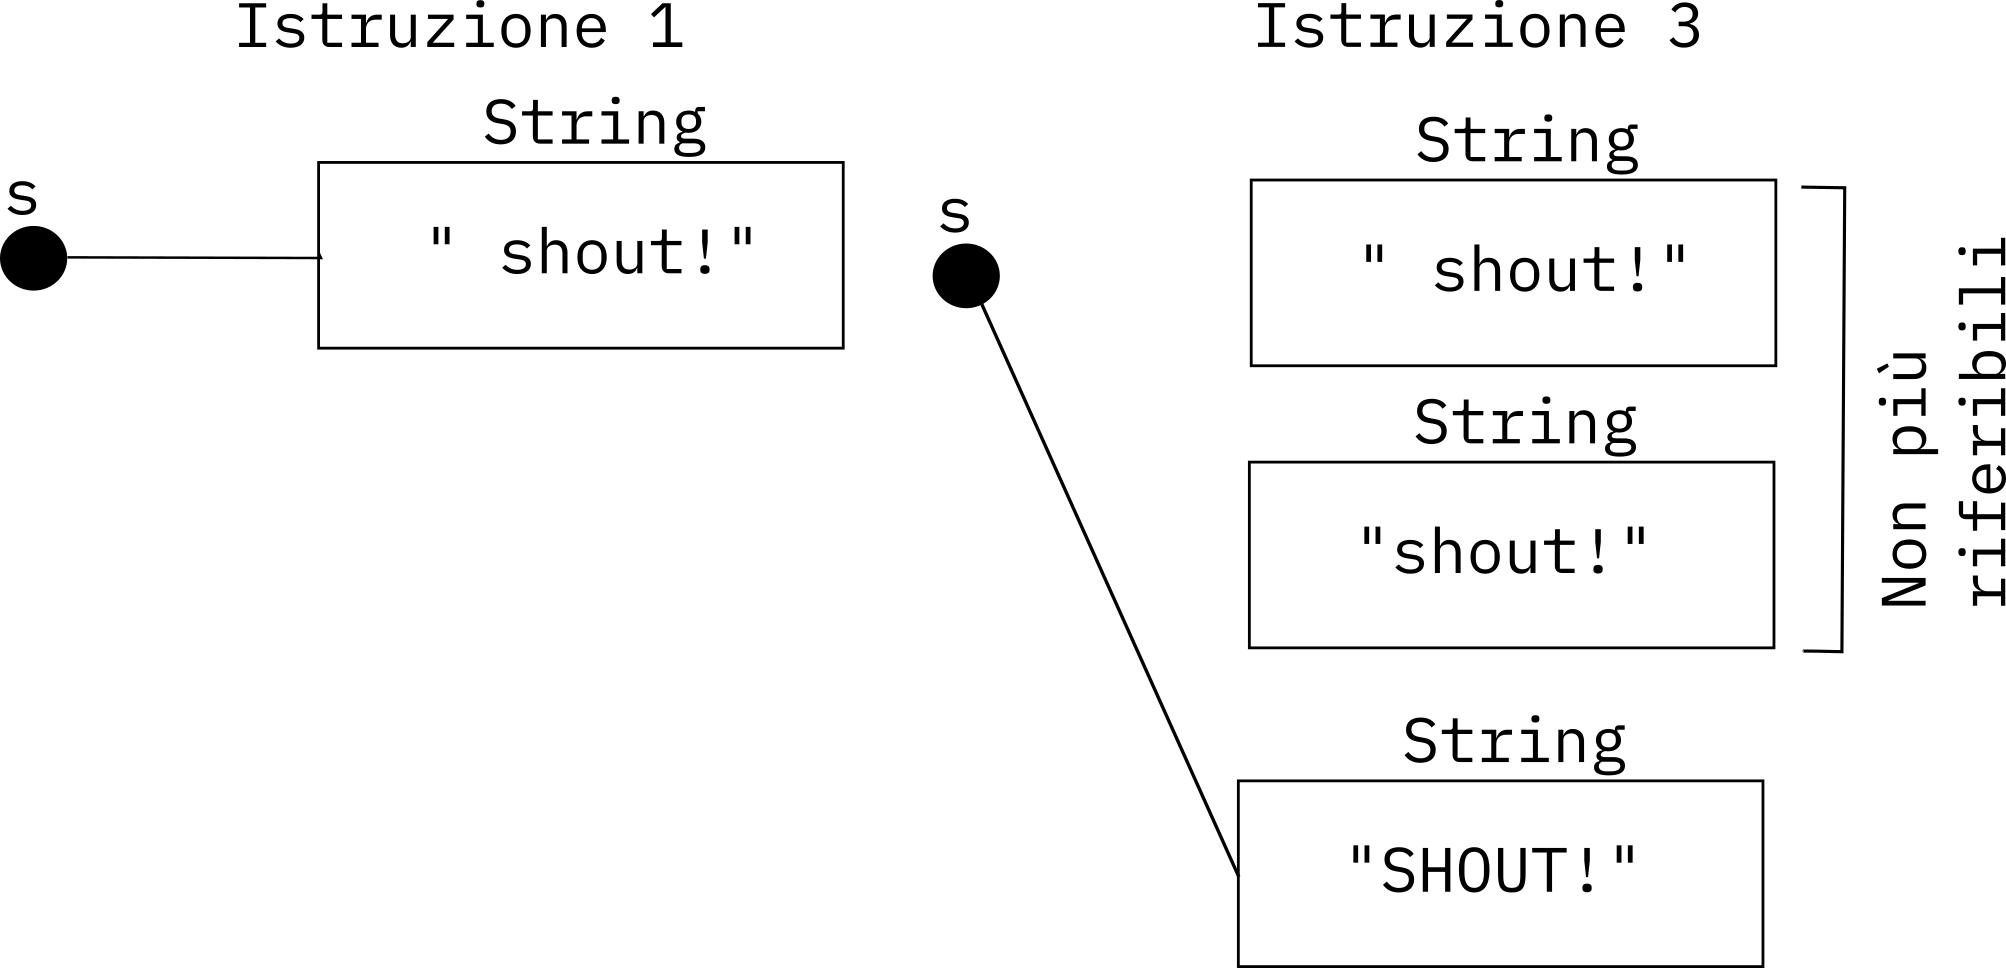
\includegraphics[ width=.7\linewidth, height=\textheight, keepaspectratio]{./pics/paintings/snippet59.png}
    \caption{Creazione di oggetti multipli nel semplice contesto di una
    creazione di un oggetto e di un'assegnazione dove sono invocati dei metodi
dell'oggetto. Ciò avviene poiché la classe \texttt{String} è
\emph{immutabile}.}
    \label{fig:snippet59}
\end{figure}




\section{Il costrutture}

Ogni classe ha \emph{almeno} un \textbf{costruttore}. Un costruttore di una
classe \texttt{T} è un metodo speciale che, quando invocato, ha come risultato:

\begin{itemize}
	\item la \emph{creazione} di un nuovo oggetto di classe \texttt{T};
	\item l'\emph{inizializzazione} del nuovo oggetto.
\end{itemize}

Un costruttore viene invocato con lo scopo di istanziare un oggetto di una
classe. I costruttori hanno vincoli \emph{sul nome} e sul \emph{parametro di
uscita} \--- il nome del costruttore è \emph{uguale al nome della classe},
mentre il parametro di uscita deve essere \emph{dello stesso tipo della
classe}. La sintassi speciale per l'invocazione del costruttore è tramite la
keyword \texttt{new}, che viene adoperata come negli esempi precedenti. Un
esempio di sintassi potrebbe essere il seguente,

\begin{lstlisting}
Greeter greeter = new Greeter();
\end{lstlisting}

L'uso della keyword è obbligatorio, con poche eccezioni, come ad esempio

\begin{lstlisting}
String s = "hi!";
\end{lstlisting}

produrrà lo stesso effetto di

\begin{lstlisting}
String s = new String("hi!");
\end{lstlisting}

All'inizializzazione, il costruttore eseguirà delle operazioni. In particolare,
per ogni tipo e per ogni classe ci possono essere più di un costruttore, spesso
con differenze proprio su come viene inizializzato un oggetto.

Supponiamo di avere una classe \texttt{Date}, che rappresenta uno specifico
istante di tempo con precisione al millisecondo. Il costruttore della classe
\texttt{Date} è così fatto,


\begin{quote}
    \footnotesize{\texttt{Date()}	Allocates a Date object and initializes it so that it represents the
    time at which it was allocated, measured to the nearest millisecond.}
\end{quote}


Il codice

\begin{lstlisting}
Date now = new Date();
// some code doing long things
Date laterThanNow = new Date();
\end{lstlisting}

con molta probabilità creerà due oggetti con stato interno diverso (la data
sarà differente).

I costruttori possono essere da $1$ singolo a molti per una singola classe.
Valgono le medesime regole dei metodi, con la lista dei parametri di ingresso
che deve essere differente per ciascuno di loro (il nome è vincolato, dunque
essi devono necessariamente differire per la lista dei parametri d'argomento).
Esempi si hanno tramite la documentazione della classe \texttt{String},


\begin{quote}
    \footnotesize{
    \texttt{String()}       Initializes a newly created String object so that it represents
an empty character sequence.

\texttt{String(char[] value)}       Allocates a new String so that it represents the
sequence of characters currently contained in the character array argument.

\texttt{String(String original)}       Initializes a newly created String object so that
it represents the same sequence of characters as the argument; in other words,
the newly created string is a copy of the argument string.}
\end{quote}


e tramite la classe \texttt{Socket},


\begin{quote}
    \footnotesize{\texttt{Socket()}        Creates an unconnected Socket.

        \texttt{Socket(String host, int port)}        Creates a stream socket and connects it to the specified port number on the named host.

    \texttt{Socket(String host, int port, boolean stream)}        Deprecated. Use DatagramSocket instead for UDP transport.

	\texttt{Socket(String host, int port, InetAddress localAddr, int localPort)}        Creates a socket and connects it to the specified remote host on the specified remote port.

    \texttt{Socket(InetAddress address, int port)}        Creates a stream socket and connects it to the specified port number at the specified IP address.

    \texttt{Socket(InetAddress host, int port, boolean stream)} Deprecated. Use DatagramSocket instead for UDP transport.

	\texttt{Socket(InetAddress address, int port, InetAddress localAddr, int localPort)}        Creates a socket and connects it to the specified remote address on the specified remote port.

    \texttt{Socket(Proxy proxy)}        Creates an unconnected socket, specifying the type of proxy, if any, that should be used regardless of any other settings.

\texttt{protected Socket(SocketImpl impl)}        Creates an unconnected Socket with a user-specified SocketImpl.}
\end{quote}



\section{Il concetto di information hiding}

L'\emph{information hiding} è il principio mediante il quale le \emph{decisioni
sul design} e sulla modellazione che subiscono frequenti variazioni vengono
nascoste all'utilizzatore, di modo da garantirne la protezione e la sicurezza
d'utilizzo nel caso in cui drastiche variazioni di design abbiano luogo. Ciò
che viene esplicitamente fornito è l'\emph{interfaccia} che tale programma
mostra nei confronti di altri programmi.

Chi crea la classe è solitamente diverso dall'utilizzatore della classe stessa.
L'utente può adoperare la classe, ma potrebbe non conoscere il codice sorgente.
Per la classe \texttt{Date}, ad esempio,


\begin{quote}
\footnotesize{
    \texttt{boolean	after(Date when)}	Tests if this date is after the specified date.

    \texttt{boolean	before(Date when)}	Tests if this date is before the specified date.

    \texttt{long	getTime()}	Returns the number of milliseconds since January 1,
1970, 00:00:00 GMT represented by this Date object.

\texttt{String	toString()}	Converts this Date object to a String of the form:
}
\end{quote}

L'idea è quella di poter effettuare operazioni apparentemente banali senza
doverci preoccupare di \emph{come} queste vengano svolte sull'oggetto: in
questo caso si parla di \textbf{information hiding}, poiché si conosce il
risultato e l'effetto di un'operazione senza conoscerne il codice sorgente o
come questa operazione venga di fatto svolta dal metodo della classe.
L'utilizzatore finale, dunque, è \emph{protetto} da qualsivoglia cambiamento
interno del modulo, protetto dal principio dell'information hiding \--- egli è
tenuto ad utilizzare soltanto ciò che viene mostrato esternamente. Lo
\emph{stato} di un oggetto e il \emph{codice} della classe potrebbero cambiare,
ma per l'utente \emph{non è necessario conoscere tali cambiamenti interni}.

L'altro aspetto dell'information hiding è la \textbf{modularità}. Un utente di
una classe conosce \emph{quali operazioni esistono, come si usano, che cosa
fanno,} tuttavia \textbf{non} sanno che cosa ci sia \emph{all'interno}
dell'oggetto, o \emph{come} esattamente funziona un'operazione.

Il concetto di modularità, dunque, si rifà alla nozione di information hiding
\--- ciascuno si prende cura di una singola parte del codice, senza che
all'utente tutto ciò non comporti alcun effetto su come vengono adoperati i
moduli stessi, poiché le interfacce esterne vengono mantenute pressoché le
stesse. Una conseguenza assolutamente notevole di ciò è che nella software
community è sufficiente che ciascuno sviluppatore si preoccupi soltanto dei
moduli di cui egli è responsabile.

\section{Riassunto del capitolo}

\begin{description}
  \item[Oggetti] Gli \emph{oggetti} sono entità che esistono, ma non hanno un nome. Essi
  sono creati in Java, manipolati attraverso il codice. 
  \item[Riferimenti] Il codice manipola gli oggetti attraverso i \emph{riferimenti}. I
  riferimenti hanno un nome, detto \emph{identificatore}, grazie al quale è
  possibile la loro manipolazione. I riferimenti possono fare riferimento ad
  oggetti esistenti e creati in precedenza.
  \item[Creazione degli oggetti e dei riferimenti] Sia i riferimenti che gli
  oggetti possono essere creati nel codice. La creazione di un oggetto prevede
  l'uso di una parola chiave, \texttt{new}, la quale fa parte del linguaggio
  Java e permette di creare un nuovo oggetto.
  \item[Associazione dei riferimenti agli oggetti] Nel codice è possibile far sì
  che i riferimenti facciano riferimento (siano associati) ad un oggetto
  esistente. In Java lo si può fare in vari modi, in particolare mediante
  l'operazione di \emph{assegnazione} (\texttt{=}) viene fatto si che il
  riferimento faccia riferimento all'oggetto indicato. Un riferimento può
  riferire ad altri oggetti durante il corso dell'elaborazione nel codice. È
  sufficiente riassegnarlo ad un altro oggetto, o ad un altro riferimento:
  in quel caso, esso farà riferimento all'oggetto il cui riferimento che viene
  indicato nell'assegnazione fa riferimento. Più oggetti possono avere più
  riferimenti che ne fanno riferimento.
  \item[Oggetti senza riferimento] Oggetti senza riferimento non hanno nome, e
  non possono pertanto più essere manipolati attraverso il codice.
  \item[Le classi] Le classi sono i tipi in Java. Ogni classe è un tipo. Ogni
  oggetto è un'\emph{istanza} di una classe. Il riferimento fa riferimento agli
  oggetti, i quali sono istanze delle classi.
  \item[I tipi primitivi] I tipi primitivi sono $8$: \texttt{boolean},
  \texttt{char}, \texttt{byte}, \texttt{short}, \texttt{int}, \texttt{long},
  \texttt{float}, \texttt{double}.
  \item[Utilizzo delle classi] In Java, le classi si adoperano tramite i
  \emph{metodi} e i loro \emph{field}. Ogni classe può svolgere operazioni
  tramite metodi, e collezionare strutture dati tramite i suoi campi.
  \item[Operazioni sugli oggetti] Le operazioni sugli oggetti dipendono dal
  \emph{tipo} dell'oggetto. In particolare, un tipo definisce le operazioni che
  sono \emph{applicabili alle istanze}.
  \item[La \emph{dot notation}] La \emph{dot notation} consente di specificare
  un'operazione su un oggetto, oppure di invocare un field di tale oggetto.
  Tipicamente la dot notation viene applicata alle \emph{istanze} di un oggetto,
  tuttavia non mancano i casi in cui essa è da applicarsi alle \emph{classi} in
  sé (o più precisamente, ai nomi di riferimento di tale classe), come nel caso
  dei metodi dichiarati \texttt{static}.
  \item[La signature] I parametri del tipo sono indicati nella \emph{signature}.
  La signature contiene \emph{nome}, sequenza dei \emph{parametri di input}, e
  \emph{parametro di output}. Il nome della sequenza dei parametri di input non
  è rilevante.  La signature indica sia il tipo di output previsto
  dall'operazione, che il tipo di input che essa accetta. La signature di un
  metodo deve essere indicativa di cosa esso rappresenta, delle operazioni che
  esso svolge, e dovrebbe essere auto-esplicativa. Possono esistere più
  signature aventi lo stesso valore di return e lo stesso nome, tuttavia esse
  devono presentare differenti parametri di input, la cui sequenza è detta
  \emph{argomento}. La sintassi \texttt{void} consente di esprimere nessun
  valore di ritorno. Il compilatore valuta le signature, e il codice viene poi
  valutato di conseguenza.
  \item[Strong typing] Java è un linguaggio \emph{fortemente tipizzato}: ciò
  significa che, a tempo di compilazione, è effettuata la verifica
  dell'esistenza di un metodo invocato, e successivamente che i tipi di input e
  di output siano rispettati.
  \item[Overloading di un metodo] I metodi possono subire \emph{overloading}:
  più metodi possono avere lo stesso nome, ma devono differire in sequenza di
  tipi di input (differire dunque nell'argomento). Essi sono dunque un insieme
  di metodi aventi lo stesso nome.
  \item[Nomi di classi] I nomi di classi dovrebbero essere \emph{nomi di attori},
  rappresentativi dell'entità che la classe rappresenta. La naming convention è
  la \emph{upper camel case}.
  \item[Nomi di metodi] I nomi di metodi dovrebbero essere \emph{verbi di
  un'azione}: essi dovrebbero essere rappresentativi delle operazioni che i
  metodi svolgono. La naming convention per i metodi è la \emph{lower camel
  case}.
  \item[Nomi di riferimenti] I nomi di riferimenti sono coerenti con il loro
  tipo, e rappresentativi dell'uso specifico di quell'oggetto, istanza di una
  determinata classe. La naming convention per i nomi di riferimenti è la
  \emph{lower camel case}.
  \item[Dot operator associativo] Il dot operator associativo consente di
      ``concatenare'' più invocazioni di metodi, con associatività da sinistra.
      I risultati ``intermedi'', cioè che non corrispondono all'ultima
      esecuzione di metodo o riferimento a field, saranno scartati.
  \item[Costruttore] Si dice costruttore della classe \texttt{T} un metodo
      speciale che, quando invocato, crea un nuovo oggetto di classe \texttt{T}
      e lo inizializza. I nomi di costruttori sono uguali ai nomi della classe
      che li ospita. Più costruttori possono coesistere, purché essi
      differiscano nell'argomento. Ogni classe ha un costruttore predefinito,
      detto \emph{costruttore di default} \--- il costruttore di default è
      \emph{automaticamente introdotto} da Java qualora non fosse stato
      esplicitamente dichiarato. Il costruttore di default è invece
      \textbf{assente} nel caso in cui vengano dichiarati altri costruttori con
      argomento diverso. L'invocazione del costruttore avviene mediante la
      parola chiave \texttt{new}, specifica del linguaggio Java, ed
      obbligatoria nella quasi totalità dei casi, eccezion fatta per oggetti
      della classe \texttt{String}.
  \item[Information hiding] L'\emph{information hiding} è il principio mediante
      il quale le \emph{decisioni sul design} e sulla modellazione che
      subiscono frequenti variazioni vengono nascoste all'utilizzatore, di
      modo di garantirne la protezione e la sicurezza d'utilizzo nel caso
      drastiche variazioni di design abbiano luogo. Esso è importante per
      \begin{enumerate}
          \item permettere all'utilizzatore di non preoccuparsi del
              funzionamento interno di un modulo;
          \item proteggere il funzionamento interno del modulo
              dall'utilizzatore, che potrebbe farne uso improprio o imprevisto;
          \item proteggere l'utilizzatore da cambiamenti repentini del modulo,
              con interfacce che non variano mai repentinamente e servizi
              forniti all'esterno che svolgono sempre lo stesso compito durante
              il tempo di sviluppo e mantenimento del modulo.
      \end{enumerate}
\end{description}


\chapter{Codifica delle classi}

\section{Esempio: i numeri complessi}

Il seguente frammento, è un esempio di utilizzo della classe
\texttt{Complex},

\begin{lstlisting}
Complex c1 = new Complex(7.46, -3.4567);
Complex c2 = new Complex(0.1, 9.81);
Complex c3 = c1.add(c2);
// same for subtract(), multiply(), divide()
double norm = c2.getNorm();
double angle = c2.getAngle();
String s = c2.toString();
double real = c2.getReal();
double imaginary = c2.getImaginary();
\end{lstlisting}

Si definisce dunque il concetto di \emph{numero complesso} come classe, assieme
alle operazioni (metodi) che si intendono svolgere con essi. Un numero
complesso può essere costruito a partire dai numeri reali, con un numero per la
parte reale ed un altro numero per la parte immaginaria. È dunque necessario
conoscere \emph{il dominio} (dei numeri complessi), definire quali sono
\emph{le parti che compongono} tale numero complesso, e quali sono \emph{le
operazioni che si possono eseguire} con tale entità. La rappresentazione non
può mai prescindere dalle entità o dalle operazioni: in Java sono necessarie
entrambe, le prime per poter produrre una classe e degli oggetti ``reali'', le
seconde per poterle manipolare. Ecco dunque che il paradigma \emph{ad oggetti},
pietra angolare del linguaggio Java, risulta essere un efficace paradigma
\emph{di modellazione}, dove l'entità ``oggetto'' incarna un proprio stato e
delle proprie operazioni, a seconda dell'entità modellata e del tipo di oggetto
da modellare.

Il seguente codice modella la classe:

\begin{lstlisting}
public class Complex {
  private double real;
  private double imaginary;
  public Complex(double real, double imaginary) {
    this.real = real;
    this.imaginary = imaginary;
  }
  public double getReal() {
    return real;
  }
  public double getImaginary() { /* ... */ }
  public Complex add(Complex other) {
    return new Complex(
      real + other.real,
      imaginary + other.imaginary
    );
  }
  /* other methods */
}
\end{lstlisting}

dove nella prima parte vengono introdotti due \textbf{field}, uno per la parte
reale ed uno per la parte immaginaria. Viene poi definito un costruttore e due
metodi (con possibilmente altri da aggiungere). I field sono \emph{oggetti
contenuti in oggetti} (di altri tipi o dello stesso tipo) \--- i field di un
oggetto ne rappresentano e costituiscono lo \textbf{stato}. Uno stato è un
possibile valore di un'istanza appartenente all'universo dei possibili valori
di un tipo. I field sono referenziati, e sono dunque anche dotati di un
identificatore. I field hanno un tipo ed un nome del riferimento scelto
(identificatore). Essi possono essere manipolati tramite la dot notation, in
egual maniera che i metodi. Ad esempio,

\begin{lstlisting}
public Complex add(Complex other) {
  return new Complex(
    real + other.real,
    imaginary + other.imaginary
  );
}
\end{lstlisting}

dove \texttt{other} deve essere un riferimento ad un oggetto per cui possono
valere le operazioni che vengono evocate, o esistono i field richiesti. I field
sono corredati dai \textbf{modificatori d'accesso} \--- essi dichiarano
\emph{quanto visibile} è l'entità appena dichiarata nei confronti di entità
esterne, ovverosia se sia lecito accedere a tale entità tramite la dot notation
(vale per field, metodi, classi). Esistono due modificatori d'accesso:
\begin{itemize}
        \item \texttt{private}: visibile soltanto all'interno del codice della
                classe stessa, o da altre istanze della medesima classe;
        \item \texttt{public}: visibile dappertutto.
\end{itemize}
Essi vanno collocati \emph{prima} della definizione del field o del metodo. Due
esempi possono essere

\begin{lstlisting}
// File Complex.java
public class Complex {
  private double real;
  /* here real can be used */
}
/* here real can not be used */

//////////////////////////////
// File ComplexCalculator.java
public class ComplexCalculator {
  public Complex add(Complex c1, Complex c2) {
    /* here real can not be used */
  }
}
\end{lstlisting}

La scelta del modificatore d'accesso opportuno per uno specifico field dipende
esclusivamente da come vogliamo modellare il concetto di information hiding
nella classe che stiamo scrivendo. In definitiva, dipende dalla \emph{natura}
dell'entità che vogliamo modellare e che la classe rappresenta, dunque dalla
conoscenza di dominio di cui disponiamo. La regola generale è che
\begin{itemize}
        \item i field dovrebbero essere \texttt{private} \--- essi
                rappresentano lo stato interno di un oggetto, e vorremmo
                evitare che un utilizzatore esterno possa manipolarlo con esiti
                imprevisti;
        \item i metodi dovrebbero essere \texttt{public} se definiscono
                operazioni che l'oggetto deve poter svolgere, mentre dovrebbero
                essere \texttt{private} nel caso in cui l'operazione che viene
                definita è riutilizzata frequentemente da altre operazioni
                pubbliche della classe stessa e in tal caso devono essere
                invocati esclusivamente dall'interno della classe (essi sono detti metodi di
                utilità interna).
\end{itemize}

Le eccezioni notevoli, tuttavia, non mancano.
L'identificatore \texttt{this} è un identificatore speciale (una keyword) del
riferimento che fa riferimento all'oggetto stesso su cui un metodo è eseguito.
Nell'esempio

\begin{lstlisting}
public class Complex {
  public Complex add(Complex other) {
    return new Complex(
      this.real + other.real,
      this.imaginary + other.imaginary
    );
  }
}
\end{lstlisting}

l'identificatore \texttt{this} fa riferimento all'oggetto stesso, è
implicitamente definita (quando viene menzionato un field senza la dot
notation, è implicito il \texttt{this}) e permette di adoperare i field
dell'oggetto stesso. Nel caso di sopra, non c'è ambiguità e pertanto non è
necessario adoperare l'identificatore \texttt{this}. In altri casi è invece
necessario, come ad esempio nei costruttori:

\begin{lstlisting}
public class Complex {
  public Complex add(Complex other) {
    return new Complex(
      real + other.real,
      imaginary + other.imaginary
    );
  }
}
\end{lstlisting}

in questo caso non è necessario. Tuttavia, per evitare l'ambiguità,

\begin{lstlisting}
public class Complex {
  private double real;
  private double imaginary;
  public Complex(double real, double imaginary) {
    this.real = real;
    this.imaginary = imaginary;
  }
}
\end{lstlisting}

nel caso di sopra è necessario adoperare l'identificatore \texttt{this}.
Solitamente, questo caso si presenta esclusivamente all'interno di costruttori
`di routine', che spesso sono automaticamente generabili da degli IDE.


\subsection{Il diagramma oggetti-riferimenti per una classe con field}

\begin{figure}[b]
        \centering
        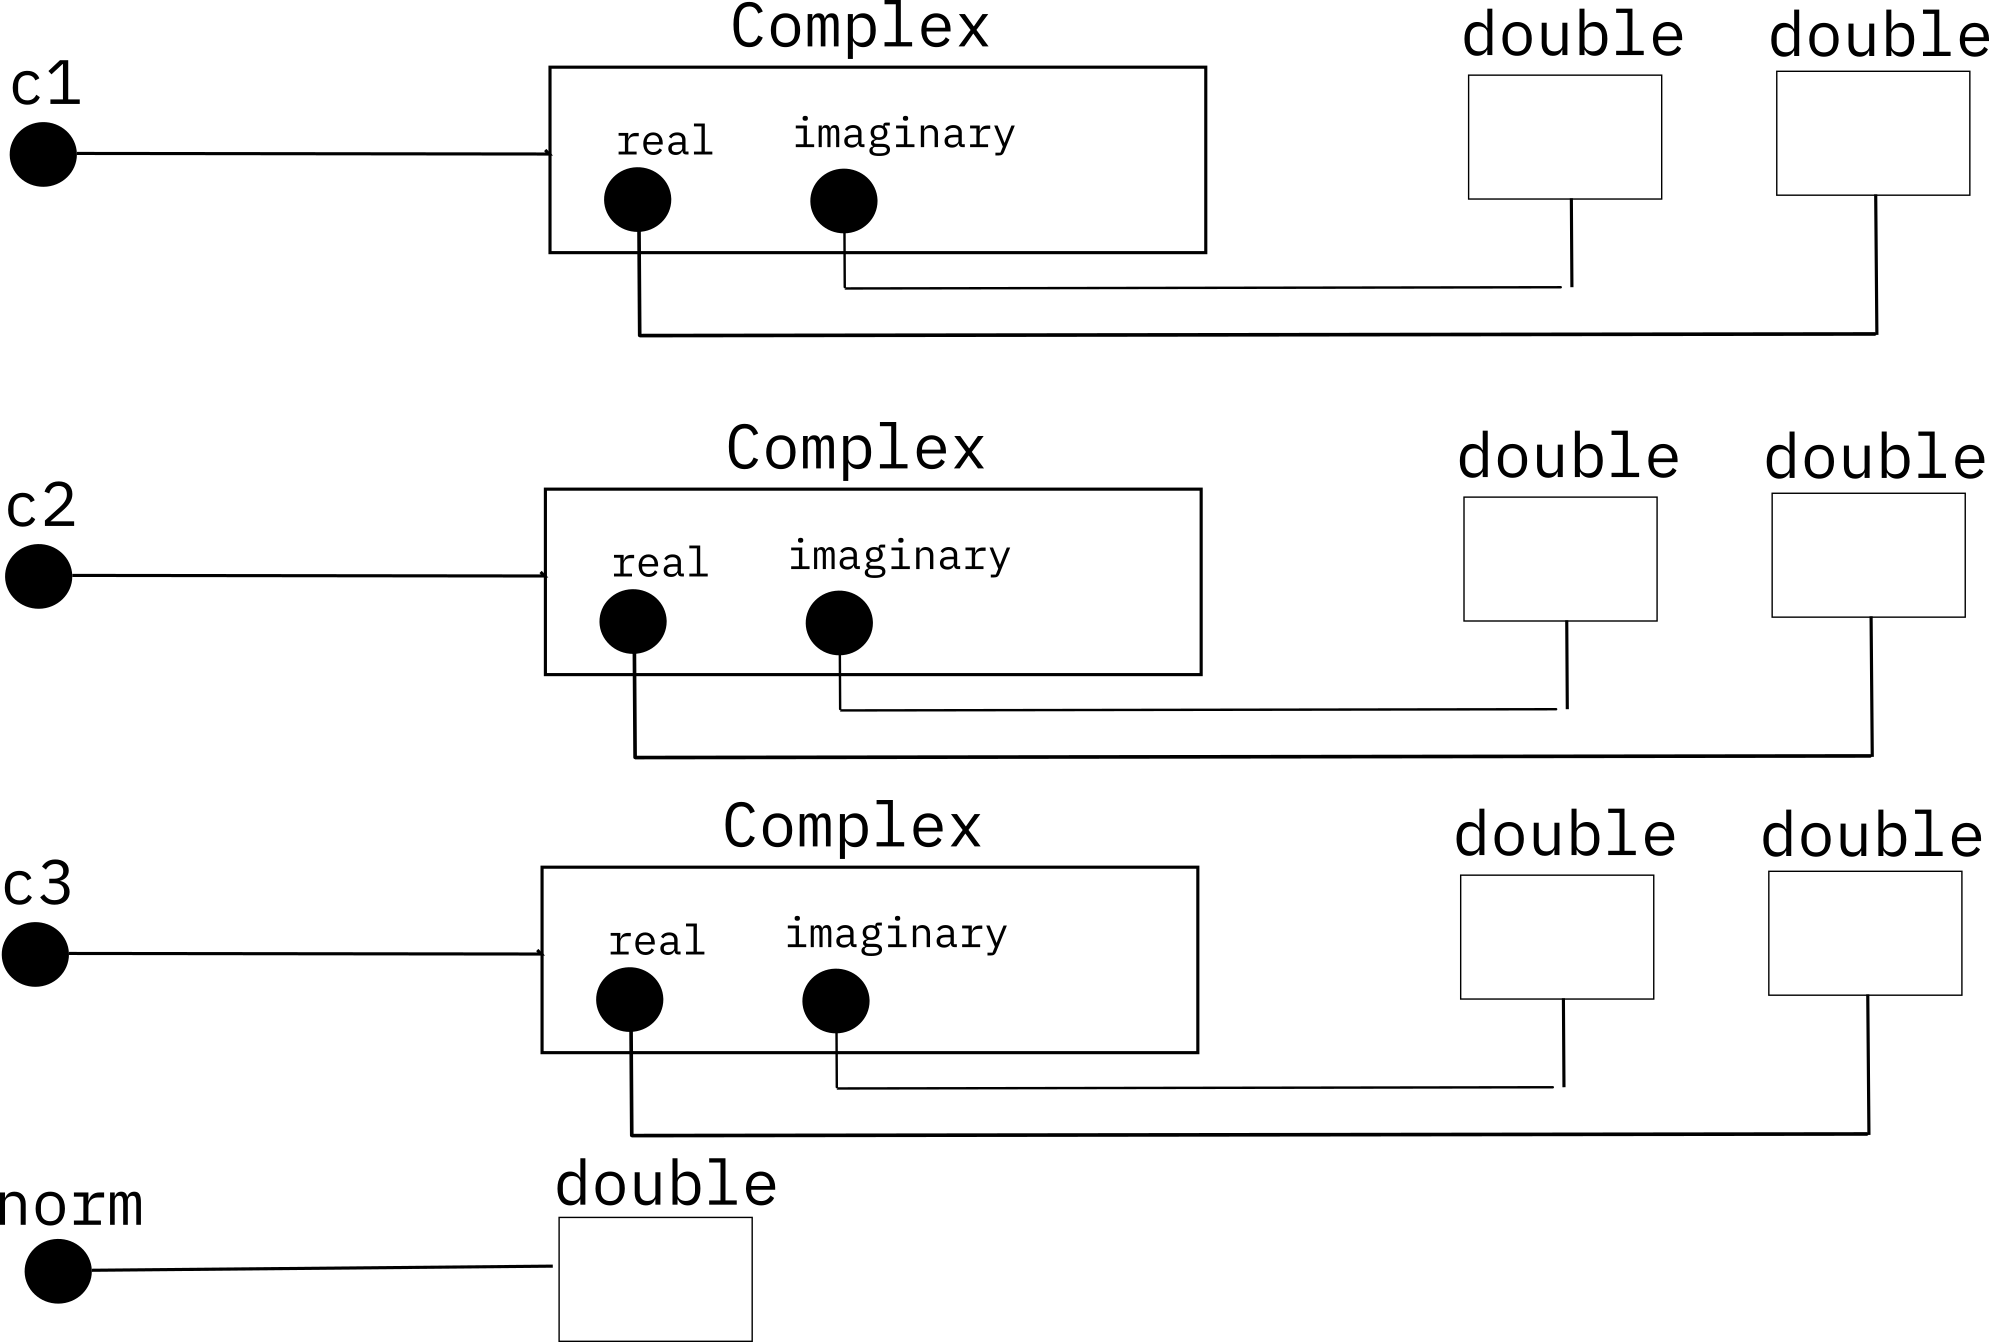
\includegraphics[ width=0.5\linewidth, height=\textheight, keepaspectratio]{./pics/png/snippet72.png}
        \caption{Diagramma oggetti-riferimenti successivamente all'esecuzione
        del codice dove vengono create tre oggetti appartenenti alla classe
    \texttt{Complex}, ed un oggetto primitivo \texttt{norm} di tipo double.}
        \label{fig:snippet72}
\end{figure}

Supponendo di eseguire il seguente codice,

\begin{lstlisting}
Complex c1 = new Complex(7.46, -3.4567);
Complex c2 = new Complex(0.1, 9.81);
Complex c3 = c1.add(c2);
double norm = c2.getNorm();
\end{lstlisting}

Nel diagramma oggetti-riferimenti, un numero complesso viene rappresentato nella
seguente maniera in Figura~\ref{fig:snippet72}.

Il contenuto degli oggetti di classe \texttt{Complex} non contiene i due
double, bensì due \emph{riferimenti ad oggetti di tipo double}. Il riferimento
\texttt{norm} viene riferito ad un nuovo oggetto di tipo double, al di fuori
degli oggetti istanziati.

Si ricorda che gli oggetti, di per sé, hanno bisogno sia di un loro \emph{stato
interno}, che di loro \emph{operazioni che possono compiere su se stessi} \---
se si rimuove qualsiasi fra le due caratteristiche, gli oggetti perdono la loro
capacità descrittiva, e diventano delle mere sequenze di funzioni (se si
tolgono i field) o delle strutture dati (se si rimuovono i metodi).

\section{Riassunto del capitolo}
\begin{description}
    \item[Paradigma ad oggetti] Il \emph{paradigma ad oggetti} è un paradigma
        di programmazione che permette di definire oggetti software in grado di
        interagire gli uni con gli altri attraverso lo scambio di messaggi \---
        le strutture dati e le procedure che operano su esse sono confinate
        all'interno di zone circoscritte del codice, dette \textbf{classi}. Le
        classi possono, infine, essere istanziate per creare gli
        \textbf{oggetti}.
    \item[Field] Un \emph{field} o \emph{campo} è un oggetto contenuto in un
        oggetto. Ciascun field può essere inteso come una vera e propria
        struttura dati in senso lato \--- si può dunque affermare che ogni
        oggetto può contenere varie strutture dati. L'insieme dei field di una
        classe è manifestazione dello \emph{stato} di una classe, un possibile
        valore di un'istanza appartenente all'universo dei possibili valori di
        un tipo. I field sono referenziati, dunque dotati di un identificatore.
        I field possono essere manipolati tramite la dot notation, similmente
        ai metodi.
    \item[Modificatore d'accesso] Un \emph{modificatore d'accesso} è una parola chiave in Java che consente di controllare la \emph{visibilità} (o \emph{scope}) di un particolare campo o metodo. Esistono tre possibili valori per la visiblità:
\begin{itemize}
    \item visibilità con modificatore d'accesso \texttt{public}: il campo o
        metodo è visibile \emph{dall'esterno} della classe; è dunque
        accessibile, modificabile o invocabile senza restrizioni si tratta di
        un metodo;
    \item visibilità con modificatore d'accesso \texttt{private}: il campo o
        metodo è visibile \emph{solo all'interno} della classe dove viene
        dichiarato. Non è dunque possibile, per un utilizzatore esterno, averne
        accesso, modificarlo o invocare il metodo;
    \item visibilità senza modificatore d'accesso, o \emph{di default}: il
        campo o metodo, in assenza di un modificatore d'accesso specificato,
        sarà visibile \emph{all'interno del pacchetto} delle classi.
\end{itemize}
    I modificatori d'accessono consentono, dunque, di modellare a nostro
    piacimento il principio dell'information hiding e decidere di mostrare o di
    celare particolari campi o metodi dall'esterno della classe. Tipicamente, i
    field dovrebbero essere \texttt{private} ed accessibili solo mediante
    metodi pubblici appositi; viceversa, i metodi dovrebbero essere
    \texttt{public}, di modo da poter essere disponibili dall'esterno, a meno che
    non si tratti di metodi di utilità interna.
    \item[L'identificatore \texttt{this}] Un identificatore di particolare
        interesse è \texttt{this}, il quale fa esplicito riferimento a
        \emph{questo} oggetto dove tale identificatore è incluso.
        L'identificatore \texttt{this} non è obbligatorio, e risulta importante
        soltanto nei casi in cui è necessario eliminare delle ambiguità, come
        nella definizione dei costruttori dove spesso i nomi dei parametri di
        input hanno lo stesso nome dei field interni.
\end{description}


\chapter{I pacchetti (packages)} 

Un certo identificatore può essere accessibile (utilizzabile), oppure
no \--- nel caso dell'identificatore \texttt{private}, il metodo o field non è
accessibile al di fuori dall'oggetto. Nel caso di metodi o campi denotati con
identificatore \texttt{public}, il file \texttt{.class} vede esportati dal
compilatore \emph{gli identificatori delle classi, dei metodi e dei field di
tale classe}. L'esportazione comprende sia i modificatori d'accesso private e
public, con private inaccessibili dall'esterno (il compilatore ci avvisa
gentilmente di ciò). Di default, il comportamento è quello di un modificatore
d'accesso \texttt{public}:

\begin{itemize}
    \item \texttt{private}: non visibile, c'è ma non si può usare;
    \item \texttt{public}: (esplicitamente) visibile;
    \item \emph{default}: (identificatore assente) visibile (all'interno del
        pacchetto).
\end{itemize}

I \textbf{pacchetti (packages)} sono un \emph{insieme} di classi con un nome.
All'interno di un package, il modificatore di accesso di default rende visibile
tale identificatore \emph{soltanto all'interno del pacchetto}. Gli
identificatori di default, benché abbiano un comportamento peculiare
all'interno del pacchetto, sono molto rari e tendono a sfavorire la modularità,
poiché non hanno un comportamento modulare corretto. Infatti, gli
identificatori di default si trovano ad essere una sorta di ``via di mezzo''
fra l'identificatore \texttt{private} e l'identificatore \texttt{public}: in
questa maniera, tendono a non avere un comportamento netto e ben definito.
Il nome di un pacchetto, dal punto di vista sintattico, è una sequenza di
lettere (token) separata da punti. Non c'è una gerarchia formale, sebbene i
nomi di pacchetti possano suggerire diversamente, per esempio osservando la
somiglianza fra i nomi di pacchetti e i nomi di dominio. I pacchetti
\texttt{java.util} e \texttt{java.util.logging} \textbf{non} hanno una vera e
propria gerarchia, non esistono sotto-pacchetti o relazioni fra pacchetti.
Tuttavia, i nomi sono scelti adoperando una \emph{convenzione}, in particolare,
vengono adoperati raggruppando i pacchetti secondo una logica non casuale.
I pacchetti sono utili per evitare il \emph{conflitto fra nomi}: due classi
aventi lo stesso nome, infatti, non potrebbero essere ``utilizzate'' assieme,
se non all'interno di differenti pacchetti. I nomi di pacchetti sono,
solitamente, in lowercase, con \emph{reverse institution/company name,
product/internal product organization}, dove il dominio con maggior grado nella
``gerarchia'' è collocato più a sinistra. I nomi dei pacchetti hanno anche un
forte impatto nell'organizzazione dei file e delle directory di lavoro Java.

\subsection{Java modules}

I \textbf{moduli}, introdotti in Java dalla versione $9$, sono molto potenti
per costruire software estremamente complesso. Tuttavia, in questo corso
saranno ignorati.

\section{Fully Qualified Name}

Unendo il nome della classe al nome del pacchetto si ottiene il \textbf{Fully
Qualified Name}, identificatore \emph{univoco} della classe. Supponendo,
dunque, per esempio un nome di pacchetto \texttt{java.net} ed una classe in
esso contenuta di nome \texttt{Socket}, il FQN corrispondente sarà
\texttt{java.net.Socket}. Mediante il FQN, ogni classe può essere univocamente
riferita da qualunque punto del codice. Ad esempio, nel frammento

\begin{lstlisting}
double r = 10;
it.units.shapes.Circle circle = new it.units.shapes.Circle(r);
double area = circle.area();
\end{lstlisting}

viene invocato il costruttore della classe \texttt{Circle} contenuta nel
pacchetto \texttt{it.units.shapes}.

\section{La keyword \texttt{import}}

I FQN rendono il codice piuttosto verboso, in quanto sarebbe molto prolisso
scrivere ogni volta da quale pacchetto vogliamo trovare una classe. Per evitare
questo fenomeno, si adopera la keyword \textbf{import}, solitamente all'inizio
del file:

\begin{lstlisting}
import it.units.shapes.Circle;
public class ShapeCompound {
  private Circle circle;
  /* ... */
}
\end{lstlisting}

La parola chiave \texttt{import} permette di scrivere soltanto \texttt{Circle}
al posto di \texttt{it.units.shapes.Circle}, e rappresenta dunque una
scorciatoia sintattica, non una qualsivoglia tipologia di
importazione\footnote{Serve soltanto al programmatore umano, per rendere
agevole la lettura del codice \--- non comporta pre-caricamento del
codice, lettura del codice, o altri effetti pratici se non quello di rendere
più agevole la scrittura del codice.}. Con \texttt{import}, dichiaro l'uso
dell'abbreviazione con il solo nome della classe, proveniente dal pacchetto
indicato. La sintassi prevede anche l'uso dell'asterisco per riferirsi a classi
multiple dello stesso pacchetto (\emph{star import}) \--- al giorno d'oggi si
evita di utilizzarlo, poiché è l'IDE a creare, in automatico, gli import
necessari al momento della scrittura del codice, e non è più richiesto
necessariamente l'intervento umano per ogni importazione. Il Fully Qualified
Name è, a volte, necessario nel caso di due \emph{classi omonime}, appartenenti
a pacchetti differenti.

Quando il compilatore processa il codice sorgente \texttt{.java} e trova una
classe \texttt{C}, egli deve conoscere i suoi metodi, e field, oltre che il
nome, la signature, e i modificatori d'accesso. C'è oltretutto una priorità con
la quale il compilatore va a cercare una determinata classe \texttt{Classname},
priva di Fully Qualified Name, nel codice:
\begin{enumerate}
    \item nel codice sorgente del file attuale \texttt{.java};
    \item nello stesso pacchetto (nella medesima directory) \--- questo rende
        non necessario porre l'\texttt{import} nel caso di classi provenienti
        dallo stesso pacchetto;
    \item nei package importati mediante star import.
\end{enumerate}

Esiste un pacchetto speciale, \texttt{java.lang}, le cui classi sono
\textbf{disponibili di default} \--- ciò equivale ad uno star import
\texttt{import java.lang.*} implicitamente presente all'inizio del file.

\subsection{Sintassi dei Fully Qualified Name}

I pacchetti e i nomi di classe non possono essere identificati soltanto
guardando il FQN. Infatti, se prendiamo come esempio
\texttt{it.units.UglySw.Point}, possono insorgere delle ambiguità:
\begin{itemize}
    \item \texttt{Point} potrebbe essere la classe;
    \item \texttt{UglySw.Point} e \texttt{UglySw} sono classi;
    \item \texttt{units.UglySw.Point}, \texttt{units.UglySw} e \texttt{units}
        sono tutte classi, mentre \texttt{it} è un pacchetto;
    \item sono tutte classi annidate.
\end{itemize}

\section{Il modificatore \texttt{static}}

Un \emph{field} di una classe C può essere definito con il modificatore di
non-accesso \texttt{static}, in modo che:
\begin{itemize}
    \item l'oggetto è \textbf{unico} per tutti gli oggetti di quell'istanza C;
    \item \textbf{esiste sempre}, anche se nessuna istanza di C viene
        istanziata;
\end{itemize}

Un field statico ha come riferimenti \emph{condivisi} con tutte le istanze della
medesima classe (potenzialmente anche nessuna istanza).

\begin{lstlisting}
public class Greeter {
  public static String msg;
  private String name;
  /* ... */
}
Greeter g1 = new Greeter();
Greeter g2 = new Greeter();
\end{lstlisting}


\begin{figure}[b]
        \centering
        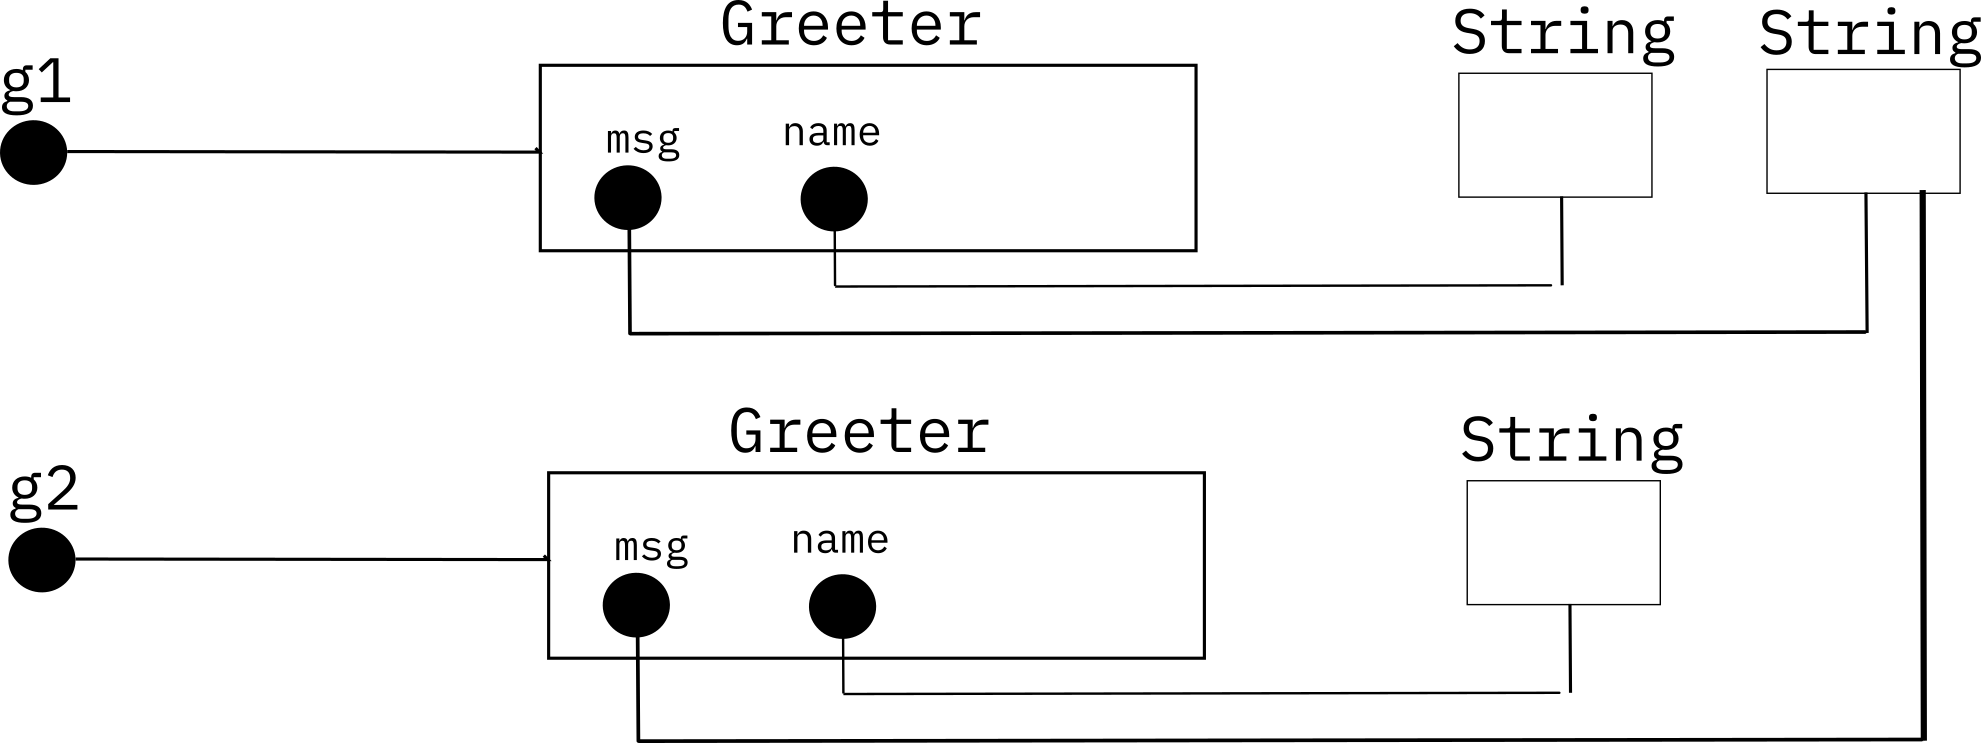
\includegraphics[ width=0.6\linewidth, height=\textheight, keepaspectratio]{./pics/png/snippet95.png}
        \caption{Relazioni fra entità con due oggetti di classe
        \texttt{Greeter} contenenti un oggetto con modificatore
    \texttt{static}.}
        \label{fig:snippet95}
\end{figure}



Anche i metodi possono essere statici. Un metodo statico:
\begin{itemize}
    \item quando invocato, non è applicato all'istanza della classe sulla quale
        è invocato. Cambia dunque, l'idea stessa di scopo ed utilizzo di un
        metodo, che non agisce più sulla medesima istanza della classe. Un
        metodo statico dunque esiste a prescindere dagli oggetti della classe a
        cui appartiene, e può essere, quasi paradossalmente, invocato
        \emph{anche quando non esiste alcuna istanza della classe a cui
        appartiene};
    \item da dentro un metodo \texttt{static} si possono adoperare
        \textbf{solo} field o altri metodi \texttt{static}: questo è
        necessario, poiché devono poter essere eseguiti anche in assenza di
        istanze (per via di questo motivo, campi e metodi non statici non
        esisterebbero). In altre parole, i metodi e i field static sono unici e
        devono poter esistere o produrre elaborazioni a prescindere dalle
        istanze della classe. La correttezza di questo assunto è verificata dal
        compilatore.
\end{itemize}

L'identificatore \texttt{static} viene adoperato facendo, per convenzione,
riferimento mediante dot notation con il \emph{nome della classe}, e
\textbf{non} con la dot notation sul riferimento che fa riferimento ad
un'istanza esistente \--- questo è fatto per evitare qualsiasi ambiguità sul
fatto che il metodo statico non può avere effetto sull'oggetto. Se infatti si
adopera la dot notation con un metodo statico su un riferimento ad un'istanza
della classe, allora si potrebbe lasciar intendere che l'oggetto in sé abbia un
ruolo nell'invocazione e nell'elaborazione del metodo statico, cosa non vera.
Gli oggetti, infatti, non hanno un vero e proprio ruolo nell'invocazione e
fungono soltanto come una sorta di ``contenitore'' dei metodi e dei field
\texttt{static}. Un metodo dovrebbe essere progettato come \texttt{static} nel
caso in cui esso rappresenti un'operazione che non coinvolga nessuna istanza di
tale classe \--- in teoria, non dovrebbe nemmeno essere definita nella classe.
Tuttavia, le operazioni sono poste in una classe piuttosto che in un'altra per
comodità e per inerenza con la classe in sé. L'identificatore static dovrebbe
anche essere adoperato per metodi \texttt{private}, qualora le condizioni di
cui sopra siano rispettate, anche se non sono disponibili al di fuori della
classe (concettualmente, vanno comunque posti come \texttt{static} per
correttezza nei confronti degli altri sviluppatori). Tipicamente, tali metodi
sono utili ad altri metodi statici. Come linea guida, se un metodo \emph{non
opera sullo stato di un'istanza di una classe}, esso dovrebbe essere
\texttt{static}.

\begin{lstlisting}
public class Dog {
  public static Dog getCutest(Dog dog1, Dog dog2) { /* ... */ }
  // Pseudo-costruttore: il nome non e' un'azione
  // serve a costruire un oggetto (createFromString, buildFromString)
  public static Dog fromString(String name) { /* ... */ }
}
\end{lstlisting}

\section{Comprensione di Hello World!}

Dato il programma ``Hello World!'',

\begin{lstlisting}
public class Greeter {
  public static void main(String[] args) {
    System.out.println("Hello World!");
  }
}
\end{lstlisting}

La signature \texttt{public static void main(String[] args)}: main è il nome
del metodo convenzionale, con nessuna variante ammessa sulla signature,
dell'\emph{entry point} dell'esecuzione sulla JVM \--- almeno una classe deve
avere un metodo \texttt{main} per poter eseguire un programma. Il metodo main
deve avere tali caratteristiche:
\begin{itemize}
    \item essere \texttt{public}: invocabile da qualunque parte, anche al di
        fuori della classe;
    \item essere \texttt{static}: deve essere invocabile senza che alcuna
        istanza di \texttt{Greeter} sia stata istanziata;
    \item non avere alcun valore di ritorno (\texttt{void}): non ritorna nulla,
        è una convenzione;
    \item soltanto \texttt{args} può essere modificato, ma per convenzione si
        lascia così com'è. Gli argomenti sono passati dal sistema operativo
        \--- nel caso non ce ne siano, l'argomento è vuoto. La separazione fra
        argomenti dipende dal sistema operativo, in Linux si separano con il
        carattere di spazio.
\end{itemize}

L'istruzione \texttt{System.out.println("Hello World!");} invoca il metodo
\texttt{println}, del field statico \texttt{out} appartenente alla classe
\texttt{System}. Un'interpretazione alternativa avrebbe potuto essere che
\texttt{println} è un metodo statico nella classe \texttt{out}, appartenente al
pacchetto \texttt{System}, ipotesi da scartare per via della convenzione che
non sarebbe rispettata nel caso di \texttt{System}, con un nome di pacchetto ad
S maiuscola e con \texttt{out} classe a lettere tutte minuscole. La classe
\texttt{System} è già presente, poiché è appartenente al pacchetto
\texttt{java.lang}, di default già importato dal compilatore. Dunque,
\texttt{java.lang.System} è il Fully Qualified Name per la classe
\texttt{System}. Guardando la documentazione per la classe \texttt{System},

\begin{quote}
    \footnotesize{\texttt{static PrintStream 	err} The "standard" error output stream.

    \texttt{static InputStream 	in} The "standard" input stream.

    \texttt{static PrintStream 	out} The "standard" output stream.
    }
\end{quote}

\texttt{out} risulta essere un field di tipo \texttt{PrintStream}, lo
``standard'' output stream\footnote{Typically this stream corresponds to
display output or another output destination specified by the host environment
or user.}.


Dentro \texttt{println} vi è una stringa, che viene immediatamente istanziata e
passata (senza riferimento) \--- \texttt{println} è un metodo che stampa una
stringa.


\begin{quote}
    \footnotesize{\texttt{void 	println(int x)} 	Prints an integer and then terminate the line.

    \texttt{void 	println(long x)} 	Prints a long and then terminate the line.

    \texttt{void 	println(Object x)} 	Prints an Object and then terminate the line.

    \texttt{void 	println(String x)} 	Prints a String and then terminate the line.
    }
\end{quote}

\subsection{Classi coinvolte}

Le classi coinvolte sono le classi definite e utilizzate. In particolare, sono coinvolte:
\begin{itemize}
    \item la classe \texttt{Greeter} definita nel codice;
    \item le classi definite altrove, ma usate nel codice sono \texttt{System},
        \texttt{String}, \texttt{PrintStream};
    \item \texttt{System} e \texttt{String} sono incluse nel pacchetto
        \texttt{java.lang}, mentre \texttt{PrintStream} è contenuta nel
        pacchetto \texttt{java.io}. Tuttavia, l'import è una scorciatoia: non è
        necessario importare \texttt{PrintStream} perché non è direttamente
        coinvolto nel codice \--- sarà invece importato o comunque presente
        nella classe \texttt{System}.
\end{itemize}

\section{Riassunto del capitolo}

\begin{description}
    \item[Pacchetti Java] Un \emph{pacchetto} o \emph{package} in Java è un
        insieme di classi dotato di un nome. Il nome di un pacchetto è una
        sequenza di token separata da punti. In Java non esiste una gerarchia
        formale fra i token, e possono essere liberamente scelti \--- gli
        sviluppatori Java, tuttavia, cercano di porre le classi all'interno dei
        pacchetti con un certo ordine. I pacchetti evitano il conflitto fra
        nomi, e raccolgono a sé varie tipologie di classi aventi funzionalità
        correlate. I nomi di pacchetti sono in lowercase, con la notazione
        \emph{reverse}: nome di compagnia/istituto, prodotto/organizzazione
        interna, nome specifico.
    \item[Fully Qualified Name] Un \emph{fully qualified name} è un
        identificatore univoco della classe all'interno dell'ambiente Java.
        Esso comprende sia il nome del pacchetto che il nome della classe,
        consentendo di eliminare ogni ambiguità nel caso di omonimie fra classi
        provenienti da pacchetti differenti. Il Fully Qualified Name è composto
        dai token del nome di pacchetto, con il nome della classe separato da
        un punto. Il FQN è necessario nel caso di ambiguità e omonimie.
    \item[La parola chiave \texttt{import}] La parola chiave \texttt{import}
        rappresenta una scorciatoia sintattica, ed indica al compilatore Java
        che sarà sufficiente scrivere il solo nome della classe al posto del
        FQN, senza dunque scrivere anche il pacchetto dal quale la classe
        proviene. Esso rappresenta soltamente un'abbreviazione, e non sta a
        significare un qualsivoglia ``import'' della classe da parte del
        compilatore, o all'inizio del file sorgente.
    \item[Lo \emph{star import}] Uno \emph{star import} è un tipo di import
        dove vengono, in un colpo solo, importate (in senso Java) tutte le
        classi appartenenti ad un pacchetto. Lo star import è effettuato
        tramite il carattere dell'asterisco, a mo' della wildcard Linux *, che
        sta ad indicare ``tutte le possibili occorrenze di un carattere o di un'espressione''.
    \item[Il caso particolare della classe \texttt{java.lang}] La classe
        \texttt{java.lang} è importata di default. Le sue classi sono dunque
        disponibili per l'uso senza indicare il FQN. È l'equivalente di uno
        star import per tale pacchetto Java.
    \item[Il modificatore \texttt{static}] Il modificatore \texttt{static} può
        essere applicato ad un metodo o un field di una classe, e si applica
        durante la definizione di esso. Introducendo un modificatore
        \texttt{static}, si dichiara che l'oggetto è \textbf{unico} per tutti
        gli elementi di quell'istanza di classe \texttt{C}, e che tale oggetto
        \textbf{esiste sempre}, prima ancora che un'istanza di tale classe sia
        stata creata. Di fatto, il modificatore \texttt{static} consente di
        produrre metodi e field che \emph{non hanno bisogno} di oggetti
        esistenti \-- tipicamente ciò è utile per creare classi di utilità o
        metodi che manipolano più oggetti. Un metodo \texttt{static} può
        operare \textbf{solo} su field dichiarati come \texttt{static}: ciò è
        desiderabile, in quanto un metodo statico non dovrebbe poter operare su
        oggetti esistenti, né dovrebbe aver bisogno di istanze della classe a
        cui appartiene. Per tale ragione e per convenzione, si è esortati ad
        invocare tali metodi \emph{direttamente sulla classe} anziché su
        oggetti istanziati (ciò è possibile in quanto ogni metodo static
        condivide i riferimenti con tutte le istanze della medesima classe),
        per evitare ogni sorta di confusione.
\end{description}



\chapter{Costruzione di una classe}

\section{Le basi della programmazione}

\subsection{Controllo del flusso d'esecuzione}

Le tipiche istruzioni di controllo del flusso sono presenti in java:
\begin{itemize}
    \item if then else;
    \item while;
    \item for;
    \item switch;
    \item break;
    \item continue;
    \item return;
\end{itemize}

\subsection{Basic Input/Output}

Tipicamente, lo standard input proviene dalla tastiera, sotto forma di caratteri
inseriti dall'utente. Lo standard output è, solitamente, anche'esso sotto forma
di caratteri, via terminale. Di solito essi sono input o output di oggetti
della classe \texttt{String} o altri tipi primitivi, anche se tipi differenti
verranno visti in futuro nel corso. Java è, solitamente, eseguito all'interno di
un \emph{terminale}. Il modo più basilare per produrre un output è quello di
utilizzare un'istanza della classe \texttt{PrintStream}: il field statico
\texttt{out}\footnote{Ci si aspetta che un'applicazione veda già il sistema
alla partenza, senza che debba essere istanziata un'entità della classe
\texttt{System}.} della classe \texttt{System}. La classe \texttt{PrintStream}
modella un \textbf{flusso} per la stampa: ha una serie di metodi, chiamati
\texttt{println}, espressi nell'elenco seguente:
\begin{quote}
\footnotesize{\texttt{void 	println()}	Terminates the current line by writing the line separator string.
\texttt{void 	println(boolean x)} 	Prints a boolean and then terminate the line.

\texttt{void 	println(char x)} 	Prints a character and then terminate the line.

\texttt{void 	println(char[] x)} 	Prints an array of characters and then terminate the line.

\texttt{void 	println(double x)} 	Prints a double and then terminate the line.

\texttt{void 	println(float x)} 	Prints a float and then terminate the line.

\texttt{void 	println(int x)} 	Prints an integer and then terminate the line.

\texttt{void 	println(long x)} 	Prints a long and then terminate the line.

\texttt{void 	println(Object x)} 	Prints an Object and then terminate the line.

\texttt{void 	println(String x)} 	Prints a String and then terminate the line.}
\end{quote}

Ugualmente, per il metodo \texttt{print}, che però non termina la linea con una
sequenza di caratteri newline. Un metodo più evoluto, \texttt{printf}, può
stampare informazioni mediante un \emph{template} predefinito (mediante
placeholders, riempiti al runtime con informazione passata come ulteriori
argomenti).

Per leggere l'input, adoperiamo un oggetto della classe \texttt{BufferedReader}:

\begin{lstlisting}
BufferedReader reader = new BufferedReader(
  new InputStreamReader(System.in) // lettore di input stream
);
/* ... */
String line = reader.readLine();
\end{lstlisting}

il metodo \texttt{readLine}, quando evocato, legge una riga e crea un oggetto
della classe \texttt{String}. La chiamata in sé richiede aggiungere
\texttt{throws Exception} dopo la signature del \texttt{main}.

L'alternativa è l'uso di un'istanza della classe \texttt{Scanner}. Lo Scanner
modella una componente software che scansiona uno stream di input alla ricerca
di sequenze di byte interessanti:

\begin{lstlisting}
Scanner scanner = new Scanner(System.in);
/* ... */
String s = scanner.next();
int n = scanner.nextInt();
double d = scanner.nextDouble();
\end{lstlisting}

Tali metodi fanno tre cose:
\begin{itemize}
    \item leggono una linea dall'\texttt{Input\-Stream} passatogli;
    \item dividono la linea in \emph{token}, col separatore spazio (\texttt{"
        "})\footnote{In alternativa, è possibile fornire un diverso
        \emph{delimiter} come argomento del metodo. Per ulteriori informazioni,
    si cerchi nella documentazione ufficiale.};
    \item converte e restituisce il primo token del tipo indicato.
\end{itemize}
Successive chiamate di next forniscono i prossimi token.

Se si adopera il BufferedReader, può essere utile adoperare i vari metodi
concatenati, come nel frammento seguente

\begin{lstlisting}
String line = reader.readLine();
int n = Integer.parseInt(line); // pseudo-constructor
float f = Float.parseFloat(String);
double d = Double.parseDouble(String);
\end{lstlisting}

\subsection{Array}

Gli array in Java sono molto simili a quelli in C. Un \textbf{array} è una
sequenza di oggetti dello stesso tipo, con lunghezza \emph{fissata} che non può
mai cambiare al runtime. Sono cosiddetti ``0-based indexing''\footnote{Questo
assunto, che per un utilizzatore di C parrebbe ovvio, non è affatto scontato:
sia il linguaggio \textsc{Matlab} che \texttt{R} fanno uso di array
``1-based'', cioè che contano a partire da 1.}. Ciascun oggetto è accessibile
mediante l'operatore \texttt{[]} applicato al riferimento. Gli array
\textbf{contengono i riferimenti}.

\begin{lstlisting}
String[] firstNames;
String[] lastNames = new String[3]; // crea array con dimensione 3 di String
lastNames[1] = new String("Medvet");
\end{lstlisting}

\begin{figure}[b]
    \centering
    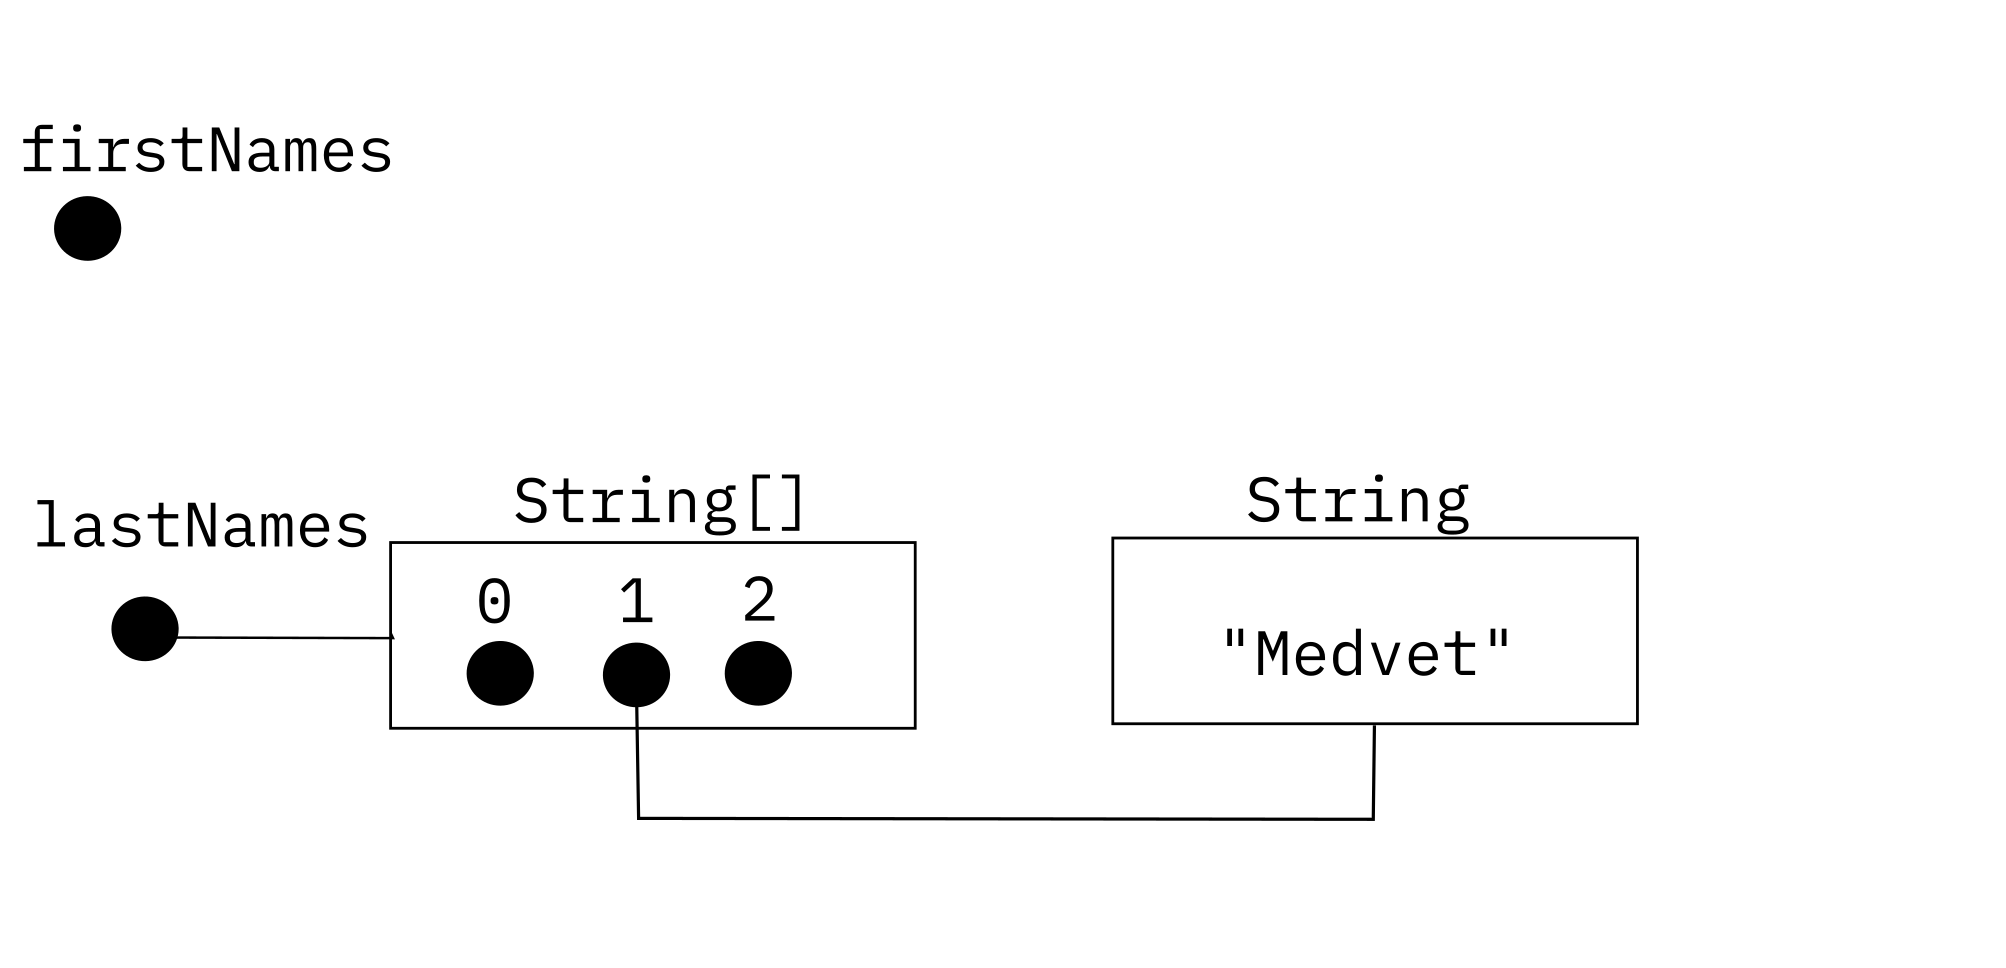
\includegraphics[ width=0.7\linewidth, height=\textheight, keepaspectratio]{./pics/paintings/snippet119.png}
    \label{fig:snippet119}
\end{figure}

Per i nomi di riferimenti ad array è, tipicamente, la \emph{forma plurale} del
nome che si darebbe al riferimento di un'istanza del tipo presente nell'array
(e.g., \emph{dog} diventa \emph{dogs}, \emph{cat} diviene \emph{cats}, e così
via). Definendo gli array, si possono adoperare due sintassi,
\begin{itemize}
    \item \texttt{Person persons[]}: fortemente sconsigliato;
    \item \texttt{Person[] persons}: fortemente consigliato;
\end{itemize}

Per creare gli array, due metodi equivalenti:

\begin{lstlisting}
String[] dogNames = {"Simba", "Gass"};
//same of new String[]{"Simba", "Gass"}
///////////////////////////////////////
String[] dogNames = new String[2];
dogNames[0] = "Simba"; //same of = new String("Simba");
dogNames[1] = "Gass";
\end{lstlisting}

Per conoscere la lunghezza di un array, esiste un field chiamato
\texttt{length}, che tuttavia può soltanto essere letto, e non modificato:

\begin{lstlisting}
String[] dogNames = {"Simba", "Gass"};
System.out.println(dogNames.length); //prints 2
dogNames = new String[3];
System.out.println(dogNames.length); //prints 3
\end{lstlisting}

\subsection{Iterazione all'interno di array}

L'iterazione su array può avvenire in due forme, una ``classica'' e una dove
avviene una semplice iterazione senza contatore e che \emph{itera su tutti gli
elementi dell'array}.

\begin{lstlisting}
String[] dogNames = {"Simba", "Gass"};
for (int i = 0; i < dogNames.length; i++) {
  System.out.println("Dog " + i + " name is " + dogNames[i]);
}
//////////////////////////////////////////
String[] dogNames = {"Simba", "Gass"};
for (String dogName : dogNames) {
  System.out.println("A dog name is " + dogName);
}
\end{lstlisting}

L'indice \texttt{i}, tuttavia, non è disponibile all'interno della seconda
iterazione.

\subsection{I varargs}

Nella signature di un metodo, l'\emph{ultimo parametro di input}, se di tipo
array, può essere specificato con tre puntini \texttt{...} anziché \texttt{[]}.
Le due istruzioni di seguito sono assolutamente equivalenti,

\begin{lstlisting}
public static double max(double... values) { /* 1 ... */}
public static double max(double[] values) { /* 2 ... */}
\end{lstlisting}

tuttavia, la seconda permette di creare un vettore opportunamente in maniera
più comoda:

\begin{lstlisting}
double max = max(4, 3.14, -1.1); //values cong double[3]; OK for 1
max = max(); //values cong double[0]; OK for 1
max = max(new double[2]{1, 2}); //Ok!; OK for 1 and 2
\end{lstlisting}

Tuttavia, c'è una limitazione importante, che sia l'ultimo parametro di input
\--- questo evita ambiguità al prezzo di espressività. Un esempio di utilizzo:

\begin{lstlisting}
public static double max(double... values) {
  double max = values[0];
  for (int i = 1; i < values.length; i++) {
    max = (max > values[i]) ? max : values[i];
  }
  return max;
}
\end{lstlisting}

Un caso in cui vi sono ambiguità nella notazione è il seguente:

\begin{lstlisting}
// does NOT compile!
public static int intersectionSize(String... as, String... bs) {
  /* ... */
}
intersectionSize("hello", "world", "cruel", "world");
\end{lstlisting}


\subsection{Command line arguments}
Disponibile soltanto come contenuto degli argomenti \texttt{main}:

\begin{lstlisting}
public class ArgLister {
  public static void main(String[] args) {
    for (String arg : args) {
      System.out.println(arg);
    }
  }
}
\end{lstlisting}

darà come output, se adoperato,

\begin{verbatim}
eric@cpu:~$ java ArgLister Hello World
Hello
World
\end{verbatim}

Un diagramma di tale esecuzione è il seguente in Figura~\ref{fig:snippet128}:

\begin{figure}[b]
    \centering
    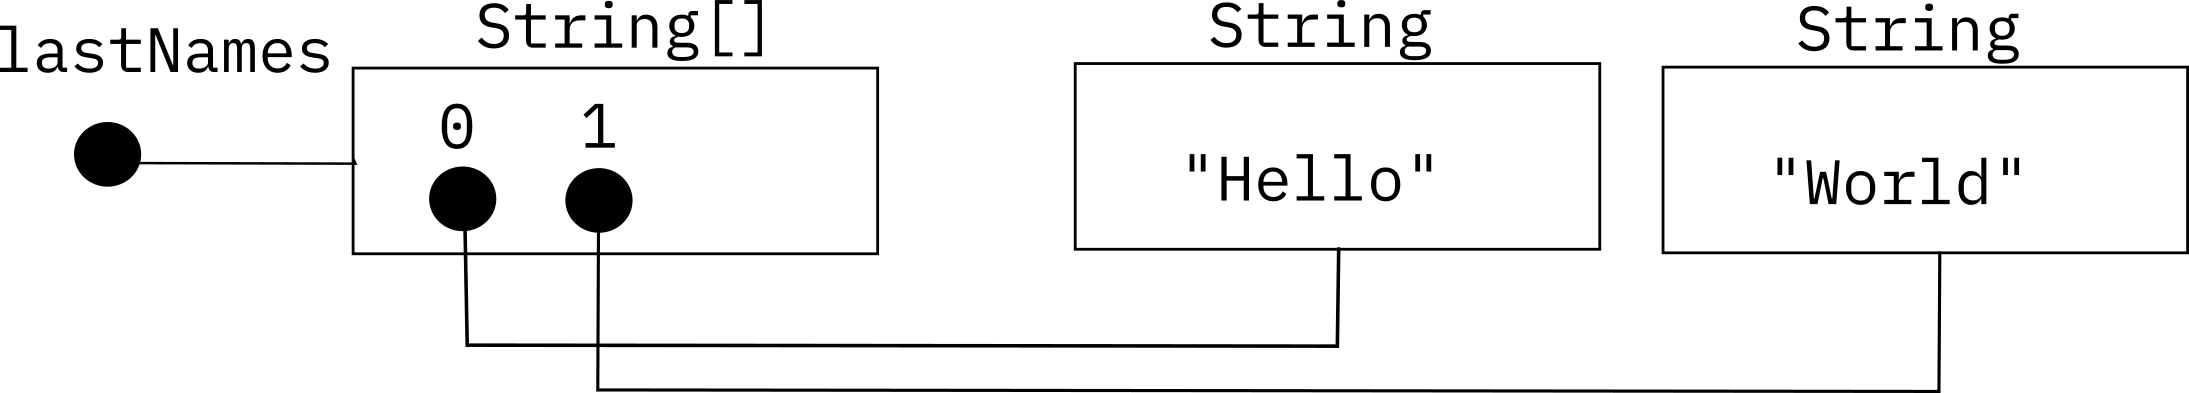
\includegraphics[ width=1.0\linewidth, height=\textheight, keepaspectratio]{./pics/paintings/snippet128.png}
    \caption{Esempio di cattura di argomenti da linea di comando.}
    \label{fig:snippet128}
\end{figure}

dove all'interno del \texttt{for} loop vi è un ulteriore riferimento, con nome di
identificatore \texttt{arg}, che riferisce, rispettivamente, al primo e al
secondo oggetto dell'array degli argomenti \texttt{args}, a seconda del ciclo.

\subsection{Operazioni fra stringhe}

Operare con stringhe si fa tramite la classe opportuna.
\begin{itemize}
    \item empty: \texttt{String s = new String()};
    \item specified: \texttt{String s = new String("hi!")};
    \item the same of \texttt{String s = "hi!"};
    \item same of another: \texttt{String s = new String(otherString)}.
\end{itemize}

Altre sono, ad esempio (slide 130),
\begin{quote}

    \footnotesize{
\texttt{int 	compareTo(String anotherString)} 	Compares two strings
lexicographically. 

\texttt{int 	compareToIgnoreCase(String str)} 	Compares two strings
lexicographically, ignoring case differences. 

\texttt{boolean 	endsWith(String suffix)} 	Tests if this string ends with the
specified suffix. 

\texttt{int indexOf(int ch)} 	Returns the index within this string of the first
occurrence of the specified character. 

\texttt{int 	indexOf(int ch, int fromIndex)} Returns the index within this string of
the first occurrence of the specified character, starting the search at the
specified index. 

\texttt{int 	indexOf(String str)} Returns the index within this string of the first
occurrence of the specified substring. 

\texttt{int 	indexOf(String str, int fromIndex)} 	Returns the index within this
string of the first occurrence of the specified substring, starting at the
specified index. 

\texttt{int 	length()} 	Returns the length of this string. 
boolean matches(String regex) 	Tells whether or not this string matches the
given regular expression. 

\texttt{String 	replaceAll(String regex, String replacement)} Replaces each substring of
this string that matches the given regular expression with the given
replacement.}
\end{quote}

Il metodo statico \texttt{format} consente di ritornare una stringa formattata
utilizzando uno specifico formato indicato nell'argomento. In pratica,
\begin{lstlisting}
String reference = String.format(
  "FPR=%4.2f\tFNR=%4.2f%n",
  fp / n,
  fn / p
);
//results in FPR=0.11 FNR=0.10
\end{lstlisting}

Le stringhe sono \textbf{immutabili}, e indicate nella documentazione come
costanti. Tuttavia, a volte la documentazione è contradditoria:
\begin{quote}
\footnotesize{\texttt{String 	concat(String str)} 	Concatenates the specified string to the end of
this string.

\texttt{String 	toUpperCase()} 	Converts all of the characters in this String to upper
case using the rules of the default locale.}
\end{quote}

Anche se, leggendo con cura, si scopre che
\begin{quote}
    \footnotesize{\texttt{public String concat(String str)}
Concatenates the specified string to the end of this string.

If the length of the argument string is 0, then this String object is returned.
Otherwise, a String object is returned that represents a character sequence
that is the concatenation of the character sequence represented by this String
object and the character sequence represented by the argument string.}
\end{quote}

Esempio con risoluzione in diagramma riferimenti-oggetti
(Figura~\ref{fig:snippet134}).

\begin{lstlisting}
// black color in diagram
String s1, s2;
s1 = "hamburger";
s2 = s1.substring(3, 7);
System.out.print("s1 = ");
System.out.println(s1);
s1 = s1.replace('a', 'b');
String[] names = { "John", "Fitzgerald", "Kennedy"};
// blue color in diagram
String firstInit, middleInit, lastInit;
firstInit = names[0].substring(0, 1);
middleInit = names[1].substring(0, 1);
lastInit = names[2].substring(0, 1);
firstInit.concat(middleInit).concat(lastInit);
\end{lstlisting}


\begin{figure}[b]
    \centering
    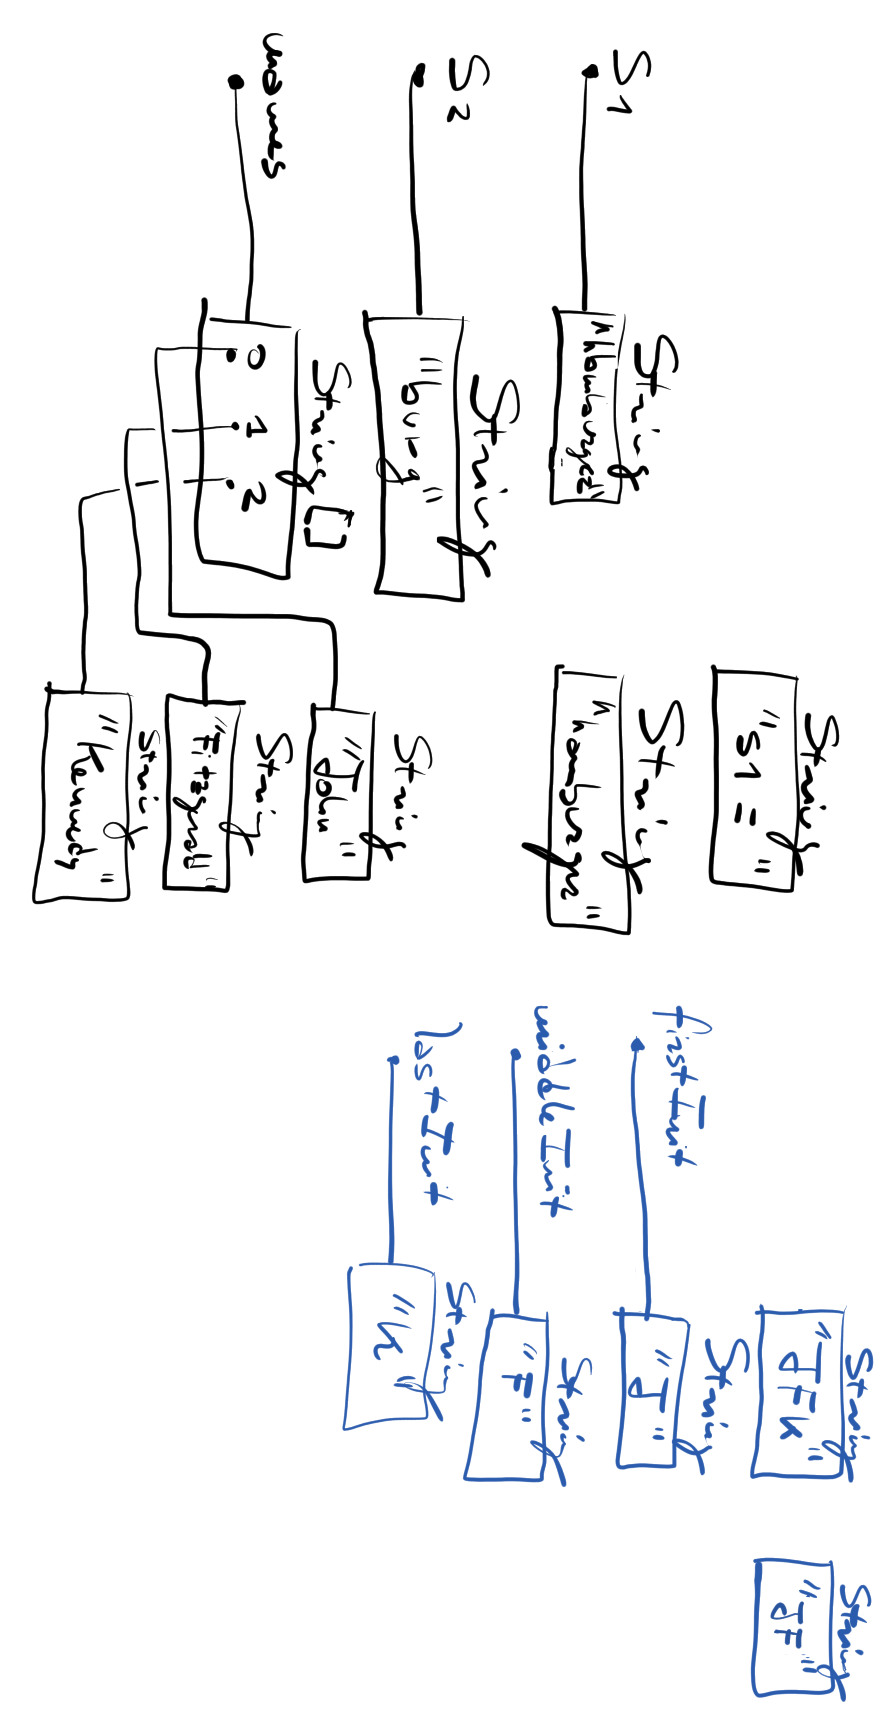
\includegraphics[ width=1.0\linewidth, height=\textheight, keepaspectratio]{./pics/paintings/snippet134.png}
    \label{fig:snippet134}
\end{figure}

\subsection{Sintassi alternativa per il metodo \texttt{concat}}

Una possibile (ed alternativa) scorciatoia sintattica per la concatenazione fra
stringhe avviene mediante l'operatore \texttt + . L'operatore \texttt + viene
valutato a partire dalla sinstra (si dirà che è \emph{associativo a sinistra}).
Alcuni esempi sono pertanto i seguenti,

\begin{lstlisting}
String s1 = "today is ";
String s2 = s1.concat(" Tuesday").concat("!");
\end{lstlisting}

che compie le stesse operazioni del frammento seguente,

\begin{lstlisting}
String s2 = s1 + "  Tuesday" + "!";
\end{lstlisting}

come la creazione degli oggetti che si avrebbero con la prima sintassi per la
concatenazione. A livello del compilatore, le operazioni eseguite sono,
infatti, le stesse: la sintassi offre soltanto all'utilizzatore un modo più
agevole (e forse più naturale) per esprimere la concatenazione fra stringhe,
benché al compilatore l'operazione risulti esattamente la stessa.

Possono essere concatenati anche operandi di tipo differente dalle stringhe. In
particolare, possiamo eseguire

\begin{lstlisting}
int age = 42;
String statement = "I'm " + age + " years old";
\end{lstlisting}

il quale dapprima convertirà implicitamente l'intero \texttt{age} nella
corrispettiva stringa, e successivamente procederà con le concatenazioni, da
sinistra verso destra. Nel caso l'operando non stringa sia un \emph{tipo non
primitivo}, il meccanismo sarà chiaro in seguito.

\clearpage

\subsection{Utilizzo dei tipi primitivi}

I tipi primitivi non vengono adoperati come gli oggetti appartenenti alle
classi. In particolare, per essi non è previsto l'uso della keyword
\texttt{new}, non hanno metodi e field e pertando non possono vedere applicata
su loro stessi la dot notation. Possono essere operandi di \emph{operazioni
binarie}, ad esempio

\begin{lstlisting}
int n = 512;
double d = 0d;
char a = 'a';
boolean flag = false;
flag = flag || true;
double k = 3 * d - Math.sqrt(4.11);
\end{lstlisting}

dove il metodo \texttt{Math.sqrt(4.11)} avrà una signature

\begin{lstlisting}
public static double sqrt(double)
\end{lstlisting}

ed apparterrà alla classe \texttt{Math}.

I tipi primitivi godono di un'inizializzazione di default. Essi, se creati ma
non inizializzati, sono inizializzati in automatico al loro valore di default:
\begin{itemize}
    \item $0$ o l'equivalente dello zero per interi, double, float e char;
    \item \texttt{false} per i booleani.
\end{itemize}

Questo però vale soltamente per i field appartenenti agli oggetti istanziati:
\textbf{non} vale per le variabili locali, le quali non vengono inizializzate e
dunque producono un errore in compilazione se utilizzate.

I tipi primitivi godono di un'inizializzazione di default anche all'interno
degli array. In particolare, durante la creazione di un array con tipi
primitivi, essi vengono posti al loro valore di default qualora non fosse
specificato altrimenti. Gli array richiedono la keyword \texttt{new}:
all'invocazione del costruttore, gli elementi interni vengono inizializzati al
loro valore di default (proprio come se fossero dei field).

\begin{figure}[b]
    \centering
    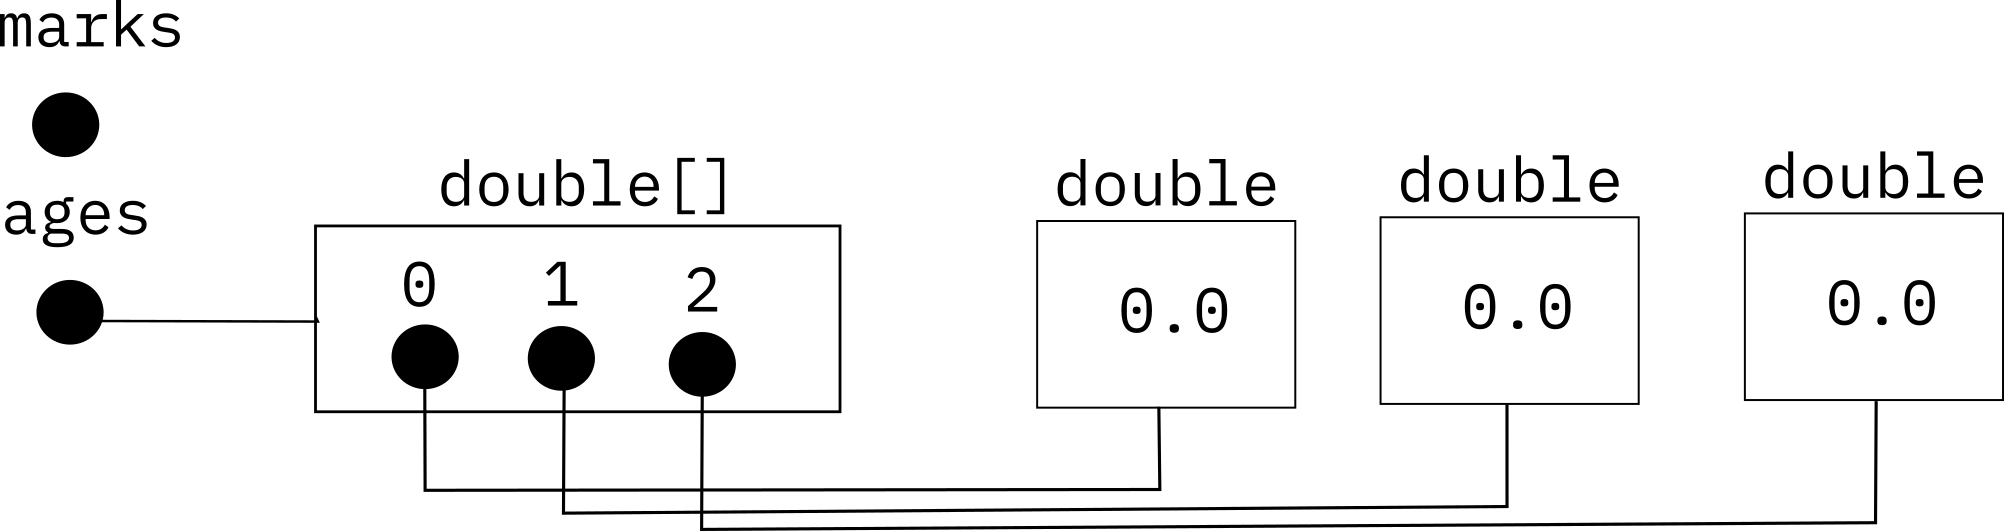
\includegraphics[ width=.8\linewidth, height=\textheight, keepaspectratio]{./pics/paintings/snippet139.png}
    \caption{Vettore di \texttt{double} inizializzato al valore di default.
    Ogni campo dell'array è inizializzato, sempre.}
    \label{fig:snippet139}
\end{figure}

I field possono essere inizializzati all'interno dell'oggetto, direttamente: si
dice che sono inizializzati \emph{inline}:

\begin{lstlisting}
public class Greeter {
  private String greet = "Hello";
  public void greet() {
    System.out.println(greet + " World!");
  }
}
\end{lstlisting}

In questa maniera, è equivalente al costruttore che produce la stessa
assegnazione, come primissima cosa\footnote{L'inizializzazione dei campi è
eseguita \emph{prima} del primo statement di qualsiasi costruttore appartenente
a quella classe}. A seguito di un'assegnazione inline, \emph{tutti gli oggetti
istanziati partono con il medesimo riferimento indicato}. Ad esempio, il
seguente codice,

\begin{lstlisting}
public class Greeter {
  private String greet = "Hello";
  private String target;
  private int n;
  public void greet() {
    System.out.println(greet + " " + target);
    System.out.println(n);
  }
}
\end{lstlisting}

produrrà il diagramma riferimenti-oggetti illustrato in
Figura~\ref{fig:snippet141}.

\begin{figure}[hb]
    \centering
    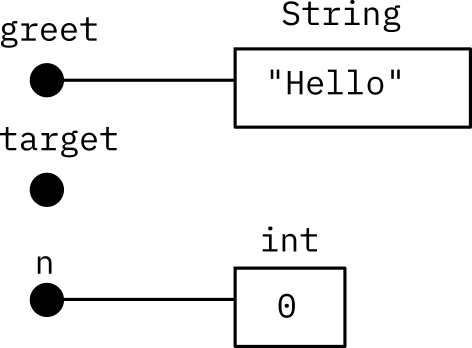
\includegraphics[ width=.55\linewidth, height=\textheight, keepaspectratio]{./pics/paintings/snippet141.png}
    \label{fig:snippet141}
\end{figure}

L'inizializzazione dei tipi primitivi avviene anche all'interno degli array. Ad esempio,

\begin{lstlisting}
int[] marks;
double[] ages = new double[3];
\end{lstlisting}

produrrà il diagramma in Figura~\ref{fig:snippet139}.


Per i tipi primitivi, l'assegnazione copia il contenuto invece che referenziare
il medesimo oggetto. Ad esempio,

\begin{lstlisting}
String s1 = "hello!";
String s2 = s1;
double d1 = 3.14;
double d2 = d1;
\end{lstlisting}

produrrà il diagramma in Figura~\ref{fig:snippet142}.
\begin{figure}[b]
    \centering
    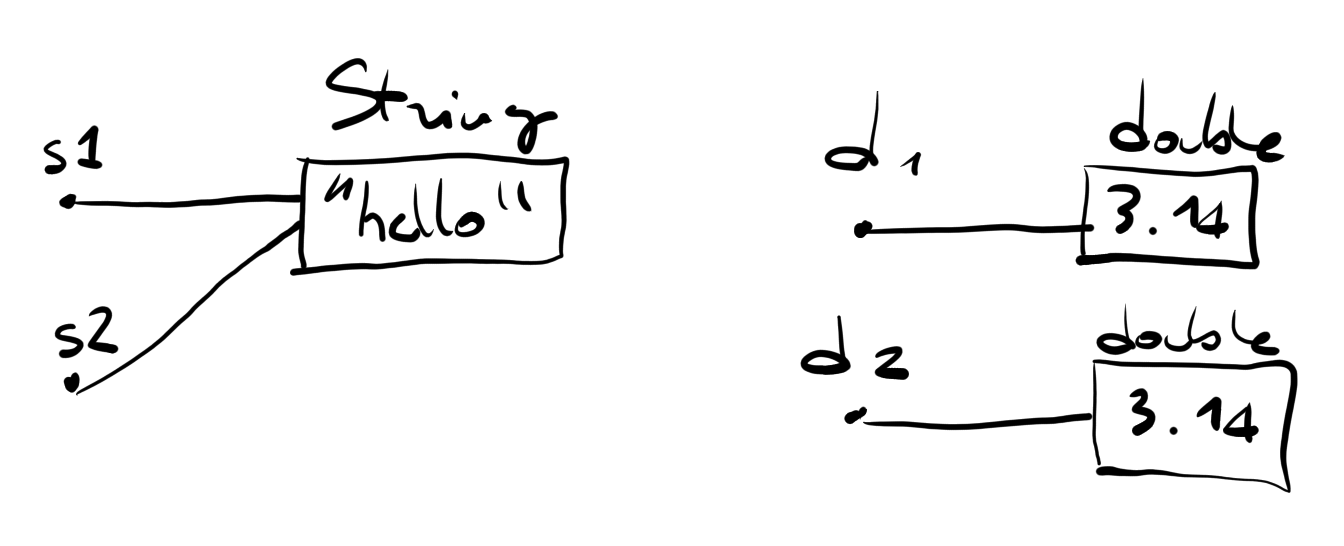
\includegraphics[ width=.6\linewidth, height=\textheight, keepaspectratio]{./pics/paintings/snippet142.png}
    \label{fig:snippet142}
\end{figure}

\subsection{Il tipo \texttt{null}}

Un tipo speciale è il tipo \texttt{null}. Si tratta di un valore speciale che
può essere referenziato da un riferimento di qualsiasi tipo non primitivo. I
field dei tipi non primitivi sono implicitamente riferiti a \texttt{null} \---
ciò avviene diversamente dai tipi primitivi, i quali sono invece impostati al
loro valore predefinito. Per le variabili locali avviene la stessa cosa: se non
inizializzate, portano ad un errore di compilazione. Qualsiasi riferimento ad
oggetto di tipo non-primitivo può \emph{esplicitamente} essere fatto riferire a
\texttt{null}, di modo che il riferimento in sé non riferisca nulla. In termini pratici,

\begin{lstlisting}
String s1 = "hi";
String s2 = null;
String s3 = null;
\end{lstlisting}

produrrà dei riferimenti s2 ed s3, i quali riferiranno ad un'area di memoria
(\texttt{null}), la quale però verrà omessa nei diagrammi per semplicità (si
dirà che non riferiscono ``a niente''). Altro esempio si ha nello snippet
seguente:

\begin{lstlisting}
public class Greeter {
  private String s1 = "hi";
  private String s2 = null;
  private String s3;
  private int n;
}
\end{lstlisting}


La dereferenziazione può anche essere valutata con l'uguaglianza \texttt{==},
in particolare si avrà

\begin{lstlisting}
String s1 = "hi";
String s2 = s1;
s1 = null;
boolean isNull = s1 == null;
\end{lstlisting}

dove il valore di \texttt{isNull} sarà \texttt{true}.

\section{Riassunto del capitolo}

\begin{description}
    \item[Input] L'input in Java proviene solitamente dalla tastiera, sotto
        forma di caratteri inseriti dall'utente. Un input che proviene da
        tastiera (se si preferisce, da terminale) è detto \textbf{standard
        input}. Vi sono due modi per ``catturare'' lo standard input, il primo
        è mediante un'istanza della classe \texttt{BufferedReader}, il secondo
        mediante un'istanza di \texttt{Scanner}.
    \item[Output] L'output in Java è solitamente anch'esso sotto forma di
        caratteri testuali su terminale, e viene pertanto detto
        \textbf{standard output}. Lo standard output può essere prodotto
        mediante un'istanza della classe \texttt{PrintStream}, ad esempio con
        il metodo \texttt{print()} o \texttt{println()}; in alternativa e per
        compiti più complessi, si utilizza il metodo \texttt{printf()}, sempre
        appartenente alla medesima classe.
    \item[Array] Gli array in Java hanno \emph{lunghezza fissata}, sono
        ``0-based'' (contano gli elementi a partire da 0) e contengono i
        riferimenti ad oggetti di un determinato tipo. Tipicamente, per i nomi
        di array si adotta il \textbf{plurale} della parola che denota gli
        oggetti che l'array contiene. Di indiscussa utilita vi è il field
        \texttt{length}, il quale ci fornisce la lunghezza del vettore in
        questione.
    \item[Iterazione su array] Oltre alla ``classica'' forma di iterazione su
        array con ciclo \texttt{while} o \texttt{for} (chi conosce il C la
        dovrebbe già padroneggiare), esiste una seconda possibilità, con il
        cosiddetto \emph{iteratore} \-- un iteratore è un oggetto del medesimo
        tipo contenuto nell'array che, in un ciclo \texttt{for}, va a pescare
        uno ad uno tutti gli elementi dell'array, con indice in ordine
        crescente. Attenzione, perché così facendo l'indice non sarà
        disponibile all'interno del ciclo \texttt{for}, cioè non sappiamo
        esattamente a che iterazione siamo (se abbiamo bisogno di saperlo,
        faremo un'iterazione alla vecchia maniera).
    \item[I \texttt{varargs}] I \texttt{varargs}, abbreviazione di
        \emph{var}iable \emph{arg}ument\emph{s}, permettono di inserire un numero arbitrario di parametri di input, purché siano rispettate determinate condizioni:
\begin{itemize}
    \item l'\textbf{ultimo} parametro di input è di tipo \emph{array};
    \item i parametri in argomento sono del medesimo tipo;
    \item vi è un \textbf{solo ed unico} \texttt{vararg} nella signature di un
        metodo.
\end{itemize}
    Dunque, un \texttt{vararg} si definisce con la sintassi \texttt{double...
    values} anziché \texttt{double[] values}, e ha la particolare utilità di
    poter definire un nuovo oggetto \emph{anche} solo ponendo i valori
    dell'array direttamente nell'argomento, ad esempio così: \texttt{double max
    = max(4, 3.14, -1.1);}.
\item[Parametri a linea di comando] Java supporta il passaggio di parametri di
    riga di comando. Essi sono contenuti nel \texttt{main}, più precisamente
    nel vettore \texttt{args[]}, a partire dall'indice 0. Si osservi che essi
    sono oggetti di tipo \texttt{String}, \emph{separati da spazi}.
\item[Operazioni fra stringhe] Le operazioni fra stringhe che siano degne di
    nota si trovano tutte nella documentazione. Tuttavia, è utile rimarcare la
    scorciatoia sintattica per il metodo \texttt{concat()}, rappresentata
    dall'operatore ``\texttt{+}'' fra stringhe \-- l'operatore prende due
    stringhe, e le \emph{concatena}. L'operatore è anche in grado di
    concatenare stringhe e oggetti di altro tipo: lo fa, infatti, invocando
    implicitamente il metodo \texttt{toString()} dell'oggetto in questione.
\item[Inizializzazione dei tipi primitivi] I tipi primitivi hanno come
    inizializzazione un valore di default, naturalmente supponendo di non
    fornirne uno noi. Per i numeri il valore di default equivale allo `zero'
    (\texttt{0} per gli interi, \texttt{0.0} per i numeri con la virgola
    mobile, e così via), mentre per i \texttt{boolean} il valore di default è
    \texttt{false}. Un po' di attenzione va prestata al caso dei \texttt{char}:
    essi sono inizializzati al corrispondente carattere codificato con lo
    `zero', in questo caso \texttt{'\textbackslash u0000'}, che corrisponde al
    carattere \texttt{null} che di fatto non è stampabile (non si può stampare
    il `niente'). I tipi primitivi godo \textbf{sempre} di un'inizializzazione
    di default, siano essi collocati all'interno di array o come field di
    oggetti. In questo ultimo caso, si possono inizializzare dentro l'oggetto
    (anche quindi non all'interno del costruttore), pertanto si dirà che essi
    sono inizializzati \textbf{inline}. L'inizializzazione inline corrisponde a
    porre i valori indicati ai field come \emph{prima} azione all'interno di un
    costruttore qualsiasi.
\item[Inizializzazione dei tipi non primitivi] I tipi non primitivi non godono
    di un'inizializzazione di default. I riferimenti ad oggetti di tipo non
    primitivo che non sono stati inizializzati faranno riferimento a
    \texttt{null}.
\item[Assegnazione di un tipo primitivo] L'assegnazione per i tipi primitivi
    copia il valore, non il riferimento (diversamente da quanto accade per gli
    oggetti di tipo non primitivo).
\item[Il tipo \texttt{null}] Il tipo \texttt{null} rappresenta \emph{il nulla}.
    Esso è un valore speciale che può essere referenziato da un riferimento di
    qualsiasi tipo, non primitivo. Invocare qualcosa che fa riferimento a
    \texttt{null} comporta un errore di compilazione. Esiste un metodo
    apposito, \texttt{isNull()}, che ci fornisce un booleano e che ci consente
    di capire se un oggetto in particolare è \texttt{null} oppure no. Il metodo
    \texttt{isNull()} fa parte della classe \texttt{Objects}.
\end{description}


\chapter{Ereditarietà delle classi}

Sia dato il seguente frammento di codice, dove viene definita la
classe \texttt{Greeter}, che compie un ``saluto''

\begin{lstlisting}
import java.util.Date;
public class Greeter {
  public static void main(String[] args) {
    System.out.print("Hello World! Today is: ");
    System.out.println(new Date());
  }
}
\end{lstlisting}

Esso produrrà un output della forma:
\begin{verbatim}
  eric@cpu:~$ java Greeter
  Hello World! Today is: Mon Mar 16 10:36:13 UTC 2020
\end{verbatim}

In parole povere, il codice stampa una \emph{data}. Il metodo \texttt{println},
stampa varie cose, fra cui, secondo la documentazione,
\begin{quote}
    \footnotesize{\texttt{void	println()}	Terminates the current line by writing the line separator string.

        \texttt{void	println(boolean x)}	Prints a boolean and then terminate the line.

        \texttt{void	println(char x)}	Prints a character and then terminate the line.

        \texttt{void	println(char[] x)}	Prints an array of characters and then terminate the line.

        \texttt{void	println(double x)}	Prints a double and then terminate the line.

        \texttt{void	println(float x)}	Prints a float and then terminate the line.

        \texttt{void	println(int x)}	Prints an integer and then terminate the line.

        \texttt{void	println(long x)}	Prints a long and then terminate the line.

        \texttt{void	println(Object x)}	Prints an Object and then terminate the line.

    \texttt{void	println(String x)}	Prints a String and then terminate the line.}
\end{quote}

Si osservi il fatto che, nello specifico, \emph{non esiste} un \texttt{println}
in grado di ricevere un oggetto di tipo \texttt{Date}, cioè nella documentazione
non esiste una voce che illustra un metodo \texttt{println} avente nella
signature un argomento di classe \texttt{Date}.

Similmente, il seguente frammento

\begin{lstlisting}
  import java.util.Date;
  public class Greeter {
    public static void main(String[] args) {
      System.out.println("Hello World! Today is: " + new Date());
    }
  }
\end{lstlisting}

produce un output della forma
\begin{verbatim}
eric@cpu:~$ java Greeter
Hello World! Today is: Mon Mar 16 10:36:13 UTC 2020
\end{verbatim}
dove la data è, almeno in apparenza, trasformata in qualche sorta di oggetto \texttt{String}. 

L'\textbf{ereditarietà} è una proprietà \emph{statica} del linguaggio \--- essa
ha effetto al \emph{tempo della compilazione}. Essa rende possibile definire un
\textbf{nuovo tipo a partire da un tipo preesistente}, specificando \emph{solo
le parti nuove o modificate}. Soltanto dunque le nuove parti, metodi e campi,
saranno definiti. La sintassi è la seguente: si aggiunge la parola chiave
\texttt{extends}, seguita dall'identificatore del tipo che si intende estendere.
Ad esempio,

\begin{lstlisting}
  public class Derived extends Base {
    /* ... */
  }
\end{lstlisting}

la classe \texttt{Derived}, appena definita, estende \texttt{Base} \--- i metodi
e i campi preesistenti saranno \emph{ereditati} dalla classe \texttt{Derived}.
Una conseguenza di tutto ciò è che non si possa ``de-definire'' metodi esistenti
nella classe \texttt{Base}. Nella definizione di tale classe che estende, sarà
possibile fare due cose:
\begin{itemize}
  \item definire \textbf{nuovi} field e metodi \--- metodi e field non possono
  essere nascosti o rimossi;
  \item \textbf{ridefinire} field e metodi.
\end{itemize}

Si dice che la classe \texttt{Derived} \textbf{estende}, \textbf{eredita} o
\textbf{deriva da} \texttt{Base}.

\subsection{La classe \texttt{Object}}

Esiste una classe particolare in Java, definita nella JVM: la classe
\texttt{Object}. Ogni classe in Java eredita da \texttt{Object} \--- se è assente, in
automatico eredita da Object. I due frammenti seguenti sono perfettamente
equivalenti:

\begin{lstlisting}
public class Greeter {
  /* ... */
}
\end{lstlisting}

\begin{lstlisting}
public class Greeter extends Object {
  /* ... */
}
\end{lstlisting}

Dunque, la classe \texttt{Object} è alla radice della gerarchia delle ereditarietà.
Se definiamo una classe con extends,

\begin{lstlisting}
public class EnhancedGreeter extends Greeter { /* ... */ }
\end{lstlisting}

possiamo dire che esiste una relazione ad `albero di ereditarietà' fra
EnhancedGreeter e Greeter, con la radice di tale albero che eredita dalla classe
Object. Altri esempi possono essere la classe \texttt{BufferedReader}, la quale
eredita dalla classe \texttt{Reader}, la quale a sua volta avrà tutti i metodi
della classe radice Object. Ciò però, dal punto di vista dello sviluppatore di
una ipotetica classe \texttt{Base}, non comporta alcuna differenza: la classe
\texttt{Base} non dovrà preoccuparsi se qualcuno, in futuro, estenderà mai la
classe. Dal punto di vista dello sviluppatore di \texttt{Derived}, invece, è
necessario conoscere la classe \texttt{Base}. Non è tuttavia necessario
conoscere il codice sorgente, i field ed i metodi \texttt{private}, o come sono
implementate le funzionalità \--- in generale, sarà soltanto necessario
conoscere i metodi ed i campi pubblici. Trattasi di un esempio di modularità,
detto \emph{separation of concerns}. In Java, infine, \textbf{non esiste
l'ereditarietà multipla}: si può estendere una sola classe.

Un problema non banale è invece l'invocazione del costruttore: chi inizializza i
campi della classe da derivare? Ad esempio,

\begin{lstlisting}
  public class Derived extends Base {
    public Derived() {
      /* init things */
    }
  }
\end{lstlisting}

con quale sistema viene inizializzato lo stato dell'istanza Derived, dal momento
in cui esso contiene anche le funzionalità di Base? Le funzionalità di Base
adoperate da Derived, infatti, assumono che la classe Base sia stata
inizializzata. Come è possibile dunque inizializzare la porzione ereditata? Il
meccanismo è quello di una \emph{invocazione implicita del costruttore di
default}, aggiunto implicitamente qualora non presente nel codice. Il
compilatore, in assenza di un metodo di costruzione esplicito, assume che la
prima azione da intraprendere (il primo statement del costruttore) sia evocare
il costruttore nullo per la classe Base. 

Cosa accade però se nella classe Base non è presente il costruttore senza
argomenti (esso potrebbe non esistere)? In tal caso, il costrutture di default
non può essere invocato, e \emph{il codice non compila}: lo sviluppatore dovrà
provvedere a fornire un costruttore adeguato per Base all'interno del
costruttore di Derived. 

La sintassi è tramite la parola chiave \texttt{super}:

\begin{lstlisting}
  public class Greeter {
  public Greeter(String name) {
    /* init things */
  }
}

  public class EnhancedGreeter extends Greeter {
    public EnhancedGreeter(String firstName, String lastName) {
      super(firstName + lastName);
      /* init things */
    }
  }
\end{lstlisting}

Il costruttore di default in questo caso non esiste (poiché è stato definito un
costruttore con argomento String): la parola chiave \texttt{super} consente di
evocare tale costruttore con argomento definito dentro \texttt{super}, della
classe che estende. In altre parole, \texttt{super} invoca il costruttore della
\emph{superclasse}.

Lo snippet

\begin{lstlisting}
  public class Base {
    public Base(int n) { /* ... */ }
    public Base(double v) { /* ... */ }
  }

  public class Derived extends Base {
  private int m;
  public Derived() {
    m = 0;
    super(5);
    /* ... */
  }
}
\end{lstlisting}

\emph{non compila} perché il costruttore \texttt{super} \textbf{deve} essere la
prima cosa ad essere eseguita\footnote{Base deve essere inizializzato prima di
qualsiasi altra operazione, altrimenti non si potrebbe sapere lo stato
dell'oggetto parent.}. Lo snippet seguente, allo stesso modo,

\begin{lstlisting}
  public class Base {
  public Base(int n) { /* ... */ }
  public Base(double v) { /* ... */ }
}

public class Derived extends Base {
  private int m;
  public Derived() {
    m = 0;
    /* ... */
  }
}
\end{lstlisting}

\emph{non compila} poiché non non esiste un costruttore senza argomenti.
Diversamente,

\begin{lstlisting}
  public class Base {
    public Base(int n) { /* ... */ }
    public Base(double v) { /* ... */ }
    public Base() { /* ... */ }
  }

  public class Derived extends Base {
  private int m;
  public Derived() {
    m = 0;
    /* ... */
  }
}
\end{lstlisting}

\emph{compila} poiché il costruttore di default è invece definito.

Se vi sono le inline initializations,

\begin{lstlisting}
  public static class Base {
    public int n = 1;
  }
/////
public static class Derived extends Base {
  public int m = n + 1;
}
/////
Derived derived = new Derived();
System.out.printf("m=%d%n", derived.m); // -> m=2
\end{lstlisting}

questo frammento funziona, infatti l'inizializzazione di qualsiasi campo avviene
\textbf{dopo} l'invocazione del costruttore super. In questo caso, la dot
notation \texttt{derived.n} è valida, e verrebbe valutata ad $1$.

\section{Riassunto del capitolo}

\begin{description}
    \item[Ereditarietà] Proprietà statica del linguaggio in cui è possibile
        definire un nuovo tipo a partire da un tipo esistente in precedenza. Si
        dirà che il nuovo tipo \textbf{estende} il vecchio tipo.
    \item[Sintassi dell'ereditarietà] La sintassi è aggiungere il termine
        \texttt{extends} nella definizione della classe.
    \item[Effetto dell'ereditarietà] L'effetto dell'ereditarietà è che il nuovo
        tipo \textbf{eredita} tutti i field e metodi della classe che estende.
        In parole povere, il nuovo tipo sarà dotato degli stessi metodi e
        field. Può, opzionalmente, ridefinirli \textbf{a patto che la signature
        sia la medesima}. I field o metodi pubblici non possono essere
        nascosti.
    \item[Design dell'ereditarietà] Dal punto di vista del software design,
        l'ereditarietà è un modo per estendere di funzionalità (o modificarne
        alcune) un oggetto già esistente. In particolare, sebbene lo
        sviluppatore dell'oggetto non si interessi a tutte le possibili
        estensioni, un secondo sviluppatore può preoccuparsi di una particolare
        estensione: vi è dunque una separazione dello sforzo di progettazione.
    \item[Costruttore di una classe che estende] Il costruttore di una classe
        \texttt{Derived} che estende \texttt{Base} chiamerà implicitamente il
        costruttore della classe \texttt{Base}, anche qualora non effettuato
        esplicitamente. La sintassi per una chiamata esplicita è tramite la
        parola chiave \texttt{super}, la quale ci consente di chiamare il
        costruttore con determinati argomenti della superclasse (nella
        gerarchia dell'ereditarietà). Qualora non indicato, il compilatore
        assume che sarà chiamato il costruttore nullo -- se non presente, non
        compila. La chiamata a \texttt{super} deve essere \textbf{la prima
        azione} intrapresa all'interno del costruttore della subclasse.
        Adoperando le inline inizializations, esse avvengono comunque dopo
        l'invocazione del costruttore della superclasse, dunque il codice
        compila.
    \item[La classe \texttt{Object}] La classe \texttt{Object} è la particolare
        classe dalla quale \textbf{ereditano tutte le altre classi}, ed è
        dunque collocata alla radice dell'albero dell'ereditarietà. Anche se
        non presente nella signature della classe, la classe automaticamente
        erediterà da \texttt{Object}.
\end{description}



\chapter{Il Polimorfismo}

Supponiamo di avere definito

\begin{lstlisting}
public class Derived extends Base { /* ... */ }
\end{lstlisting}

in questo caso, qualsiasi codice scritto per Base può funzionare anche con
Derived: in particolare, un riferimento al tipo Base può riferire ad un oggetto
di tipo Derived. In altre parole,

\begin{lstlisting}
public void use(Base base) { /* ... */ }

Base base = new Derived(); // OK!!!

use(new Base()); // OK, sure!
use(new Derived()); // OK!!!
\end{lstlisting}

Cambiando solo la signature, tutte le dot notations effettuate sul \texttt{Base} valgono
anche per la classe \texttt{Derived}, possiamo scambiare \texttt{Base} con \texttt{Derived} e il
compilatore non si lamenterà. Il compilatore lo ritiene legittimo, la
seconda istruzione del precedente frammento di codice compilerebbe ed
eseguirebbe senza problemi. Il metodo \texttt{use()} compila poiché è stato
scritto per funzionare con una \texttt{Base} \--- ciascun metodo o field valido nel \texttt{Base}
è anche valido per il \texttt{Derived}, anche se vi sono diversi comportamenti dei
metodi.

Filosoficamente, l'ereditarietà ci permette di instaurare relazioni fra classi,
``filosoficamente'', con una specie di \emph{sillogismo}

\begin{lstlisting}
public class LivingBeing { /* ... */ } // is an Object

public class Animal extends LivingBeing { /* ... */ }

public class Mammal extends Animal { /* ... */ }

public class Dog extends Mammal { /* ... */ }

public class Chihuahua extends Dog { /* ... */ }
\end{lstlisting}

Grazie all'ereditarietà possiamo definire \emph{gerarchie concettuali}. È
oggetto di disputa\footnote{https://qr.ae/pNnOEU} il fatto che l'ereditarietà sia la
maniera corretta per modellare tale relazione fra oggetti, poiché vi sono altri
modi per modellare questa relazione fra concetti: uno dei motivi è perché non
esiste l'ereditarietà multipla. In generale, bisogna sempre tendere ad adoperare
il livello più astratto di qualche entità, piuttosto che quello più specifico:

\begin{lstlisting}
// better
public void putLeash(Dog dog) { /* ... */ }

// not goot 
public void putLeash(Chihuahua dog) { /* ... */ }
\end{lstlisting}

Similmente,

\begin{lstlisting}
  // best
  public Milk milk(Mammal mammal) { /* ... */ }
  
  // not so good
  public Milk milk(Cow cow) { /* ... */ }
  
  // wrong!
  public Milk milk(Animal animal) { /* ... */ }
\end{lstlisting}

Una classe che estende non può rimuovere metodi della classe che estende. In
particolare, ciò renderebbe falso l'affermazione chiave dell'ereditarietà ``Ogni
Derived è un Base''. Lo stesso deve valere anche per la visibilità dei metodi di
Base, che \emph{non può essere ridotta}. La riduzione della visibilità, dunque,
\textbf{non è ammissibile in Java}.

Metodi omonimi, tuttavia, possono essere ridefiniti per buone ragioni. In
particolare,

\begin{lstlisting}
  public void greet(Person person) {
    System.out.println("Hi, " + person.getFullName());
  }

  public class Person {
    /* ... */
    public String getFullName() {
      return firstName + " " + lastName;
    };
  }

  public class Doc extends Person {
    /* ... */
    public String getFullName() {
      return "Dr. " + firstName + " " + lastName;
    };
  }
\end{lstlisting}

In questo caso siamo di fronte alla proprietà del \textbf{polimorfismo}: la
conseguenza \emph{dinamica} (al runtime) dell'ereditarietà. Il medesimo codice
può avere \emph{comportamenti diversi} al runtime a seconda del tipo effettivo
dell'oggetto che viene manipolato al momento dell'esecuzione. Naturalmente, lo
sviluppatore della classe \texttt{Derived} \textbf{deve decidere} se tale classe sia
effettivamente derivata da \texttt{Base}, oppure no: in altre parole, è compito dello
sviluppatore assicurarsi che i metodi chiamati rispettino le necessità, di modo
che possano funzionare anche sul metodo non generale con una certa, perlomeno,
somiglianza con il metodo definito in \texttt{Base}.

Il polimorfismo è conseguenza del fatto che una classe \texttt{Derived} ha le
medesime proprietà (metodi, field) degli oggetti di tipo \texttt{Base} \--- in
questa maniera, il compilatore consente allo sviluppatore di adoperare metodi
costruiti specificatamente per la classe \texttt{Base} su oggetti di tipo
\texttt{Derived}, mentre non vale il contrario, poiché la classe
\texttt{Derived} possiede metodi e field peculiari, potenzialmente in aggiunta
rispetto a quelli proposti dagli oggetti della classe \texttt{Base}.

Naturalmente, non vale il contrario:

\begin{lstlisting}
public Base createBase() { /* ... */ }
Derived derived;
derived = createBase();
\end{lstlisting}

In questo caso, \texttt{derived} contiene le proprietà degli oggetti della
classe \texttt{Derived}. Applicare il metodo \texttt{createBase} su \texttt{derived},
\emph{non compila} perché al runtime \textbf{non è garantito che un oggetto \texttt{Base}
contenga un metodo invocato con dot notation, della classe \texttt{Derived}}. Una
situazione potrebbe essere la seguente,
\nopagebreak
\begin{lstlisting}
public Base createBase() {
  if (System.currentTimeMillis() % 2 == 0) {
    return new Base();
  }
  return new Derived();
}
/////
Derived derived;
derived = createBase();
\end{lstlisting}

è un metodo maledettamente diabolico.

Esiste una sintassi per forzare la compilazione, detta \textbf{downcasting}
(rispetto all'albero dell'ereditarietà):

\begin{lstlisting}
Derived derived;
derived = (Derived) createBase();
\end{lstlisting}

dove si inserisce fra parentesi\footnote{La sintassi stessa, dove il tipo
dell'oggetto viene specificato fra parentesi, indica la precarietà intrinseca
dell'operazione.} l'identificatore del tipo di cui si intende effettuare il
cast. Il compilatore lo lascia inalterato, però al runtime potrebbe comunque non
essere un Derived (in tal caso, potremmo incappare in errori). Tale sintassi,
\begin{itemize}
  \item ``cambia'' il tipo di riferimento downcast;
  \item funziona soltanto se Derived deriva direttamente o indirettamente da
      Base -- questo poiché \texttt{createBase()} \textbf{deve} tornare un
      \texttt{Base}, dunque non è possibile accettare qualcosa che non può
      accadere;
  \item funziona solo se i tipi sono in relazione, cioè se ogni tipo in return è
  alto in gerarchia quanto il tipo dichiarato, altrimenti non compila.
\end{itemize}

Oltre alle verifiche in atto di compilazione, al runtime vi sono verifiche ad
ogni invocazione.

Le ragioni per l'uso del downcasting potrebbero essere quelle in cui un tipo
particolare è resituito, ma dipende \emph{a seconda di un parametro}.

\subsection{La sintassi \texttt{instanceof}}

La sintassi \texttt{instanceof} serve per controllare il tipo di un oggetto al
runtime. In altre parole, a sinistra abbiamo un tipo \texttt{boolean}, e alla destra vi è
un predicato (riferimento - oggetto). Nell'esempio,

\begin{lstlisting}
boolean isString = ref instanceof String;
\end{lstlisting}

\texttt{isString} è al valore \texttt{true} se \texttt{ref} è un riferimento ad
un oggetto di tipo \texttt{String}, mentre sarà di valore \texttt{false}
altrimenti.

Formalmente, \texttt{a instanceof B} è \texttt{true} se e solo se l'oggetto
riferenziato da \texttt{a} può essere legittimamente referenziato da un
riferimento \texttt{b} ad oggetti di tipo \texttt{B}. In altre parole, l'esempio
è esplicativo:

\begin{lstlisting}
public class Derived extends Base { /* ... */ }
Derived derived = new Derived();
boolean b1 = derived instanceof Object; // -> true
boolean b2 = derived instanceof Base; // -> true
boolean b3 = derived instanceof Derived; // -> true
\end{lstlisting}

Il compilatore, in certi casi di falsità tautologica, si rifiuta di compilare.
Ad esempio,

\begin{lstlisting}
Base b = new Base();
... = b instanceof String; // sempre falso, non compila!
\end{lstlisting}

L'uso tipico di \texttt{instanceof} potrebbe essere

\begin{lstlisting}
Object obj = someOddMethod();
if (obj instanceof String) {
  String string = (String) obj;
  System.out.println(string.toUpperCase());
  // obj.toUpperCase() would not compile!
}
/////
// Pattern matching
Object obj = someOddMethod();
if (obj instanceof String string) {
  System.out.println(string.toUpperCase());
}
\end{lstlisting}

con la possibilità di discernere fra vari casi e tipologie di oggetto. La
scorciatoia è elegante, e prende il nome di \textbf{Pattern matching}.

\subsection{Il caso dell'esempio della classe \texttt{Date} e il metodo \texttt{toString}}

Tornando al frammento di inizio capitolo,

\begin{lstlisting}
import java.util.Date;
public class Greeter {
  public static void main(String[] args) {
    System.out.print("Hello World! Today is: ");
    System.out.println(new Date());
  }
}
\end{lstlisting}

Esiste infatti un metodo println tale che
\begin{quote}
    \footnotesize{\texttt{void	println(Object x)}	Prints an Object and then terminate the line.}
\end{quote}
stampa qualsiasi oggetto. La classe \texttt{Object} ha un metodo di nome
\texttt{toString}. Tale metodo \emph{restituisce una rappresentazione in Stringa
dell'oggetto}\footnote{https://docs.oracle.com/en/java/javase/17/docs/api/java.base/java/lang/Object.html\#toString()}. 
In questo caso, la documentazione è fornita a due tipi di sviluppatori:
l'utilizzatore, e il designer che andrà a ridefinire il metodo. È opportuno che
tutte le classi che estendono \texttt{Object} \emph{ridefiniscano il metodo}. È anche
specificato il \emph{contratto} che deve essere rispettato nel ridefinire tale
metodo. Inoltre, vengono specificate anche le istruzioni per gli utilizzatori.
In particolare, vengono restituiti nome dell'oggetto e un suo \emph{hash}.
In via definitiva, \emph{ogni oggetto ha la capacità di essere rappresentato
come una stringa}.

Tipicamente, si desidera fare l'\emph{overriding} del metodo \texttt{toString}.
Le linee guida sono le seguenti: 
\begin{itemize}
  \item restituisce una stringa che \emph{rappresenta testualmente} l'oggetto;
  \item conciso ma informativo;
  \item sia di facile lettura per una persona umana.
\end{itemize}

Ad esempio, il metodo \texttt{toString} per la classe Date,

\begin{quote}
    \footnotesize{\texttt{public String toString()}

  Converts this Date object to a String of the form:
  
  dow mon dd hh:mm:ss zzz yyyy
  
  where:
  
  dow is the day of the week (Sun, Mon, Tue, Wed, Thu, Fri, Sat).

  mon is the month (Jan, Feb, Mar, Apr, May, Jun, Jul, Aug, Sep, Oct, Nov, Dec).

  dd is the day of the month (01 through 31), as two decimal digits.

  hh is the hour of the day (00 through 23), as two decimal digits.

  mm is the minute within the hour (00 through 59), as two decimal digits.

  ss is the second within the minute (00 through 61), as two decimal digits.

  zzz is the time zone (and may reflect daylight saving time). Standard time
  zone abbreviations include those recognized by the method parse. If time zone
  information is not available, then zzz is empty - that is, it consists of no
  characters at all.

yyyy is the year, as four decimal digits.}
\end{quote}

In definitiva, il metodo \texttt{println} per \texttt{Object} fa una cosa simile:

\begin{lstlisting}
public void println(Object x) {
  if ( x == null ) {
    println("null");
  } else {
    println(x.toString()); // esiste sempre!
  }
}
\end{lstlisting}

dove, in realtà, vi è un information hiding dove un println verifica che il
riferimento non riferisca a \texttt{null}, e poi \emph{delega} al secondo println
la stampa, e in via definitiva, a tutti gli altri sviluppatori di definire la
rappresentazione in stringa di un oggetto.

Anche la concatenazione funziona. Infatti, il compilatore adopera implicitamente
il metodo \texttt{toString} qualora servisse una stringa dell'oggetto. Ad esempio, in 

\begin{lstlisting}
  System.out.println("Now is " + new Date());
\end{lstlisting}

avviene una sorta di conversione implicita, del tipo

\begin{lstlisting}
  (ref == null) ? "null" : ref.toString()
\end{lstlisting}

In parole povere, quando necessario e quando richiesto, ciascun oggetto viene
convertito nella sua rappresentazione a stringa, mediante il metodo
\texttt{toString}.

\section{Il funzionamento del polimorfismo}

La Java Virtual Machine è in grado di effettuare il polimorfismo. Al runtime,
ogni oggetto \texttt{o} non primitivo ha un \emph{riferimento ad un field che è
la descrizione del suo tipo}. Esiste un tipo (una classe) di nome \texttt{Class}
\--- ogni oggetto ha un field di tipo \texttt{Class}\footnote{Trattasi
dell'unico caso dove un field ha il proprio nome di riferimento indicato con la
iniziale maiuscola.}, ereditato dalla classe \texttt{Object}. Inoltre, la
descrizione del tipo è la medesima per tutte le istanze della medesima classe di
\texttt{o}. In altre parole, il field \texttt{Class} è \texttt{static} con
modificatore d'accesso \texttt{private}, e può essere ottenuto mediante un
metodo della classe \texttt{Object}, \texttt{getClass}. Nella classe
\texttt{Object}, vi sarà un field del tipo

\begin{lstlisting}
  public class Object {
    private static Class<?> clazz; // set by JVM, probably wrote in bytecode directly
    public Class<?> getClass() {
      return clazz;
    }

    // metodo toString...

    // ...
  }
\end{lstlisting}

Il metodo \texttt{getClass} restituisce il \textbf{tipo al runtime} della classe
\texttt{Object}.

\begin{figure}[hb]
    \centering
    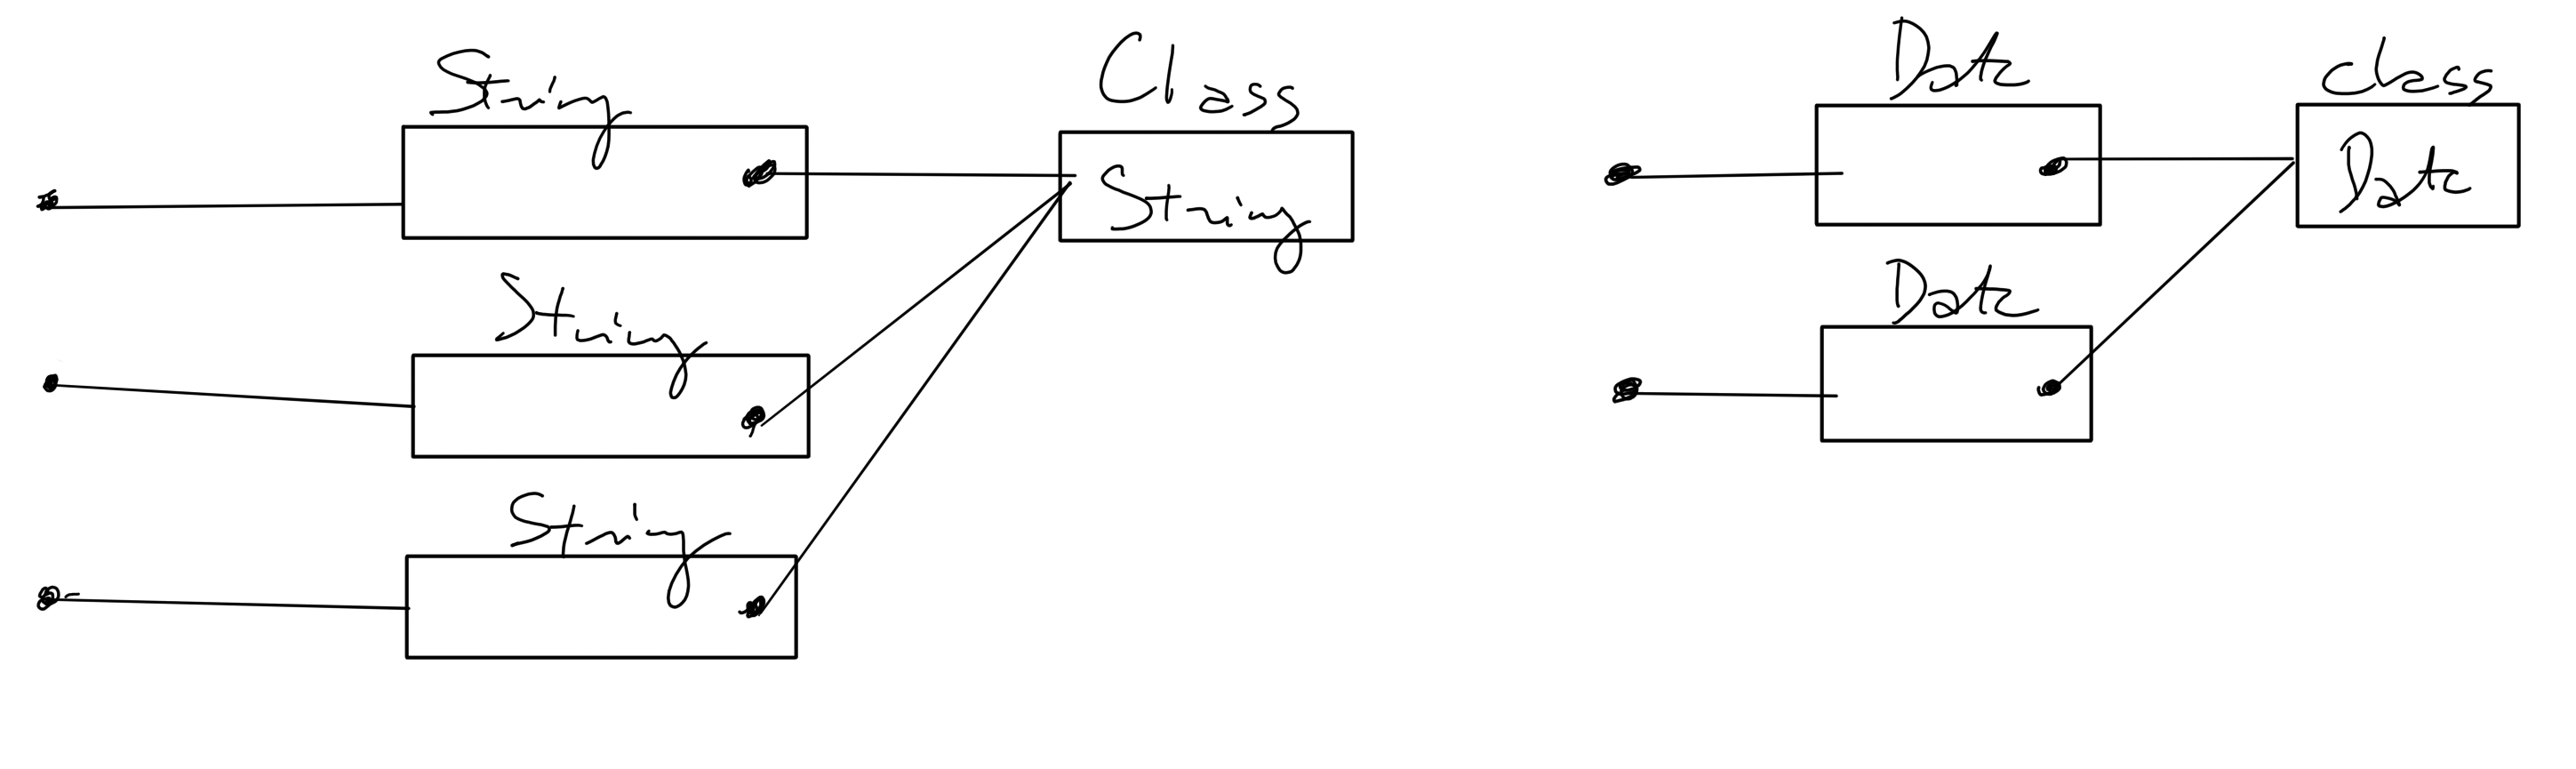
\includegraphics[ width=1\linewidth, height=\textheight, keepaspectratio]{./pics/paintings/snippet198.png}
    \caption{Presenza del field di tipo \texttt{Class} all'interno degli oggetti
    di tipo \texttt{String} e di tipo \texttt{Date}.}
    \label{fig:snippet198}
\end{figure}

\begin{figure}[hb]
    \centering
    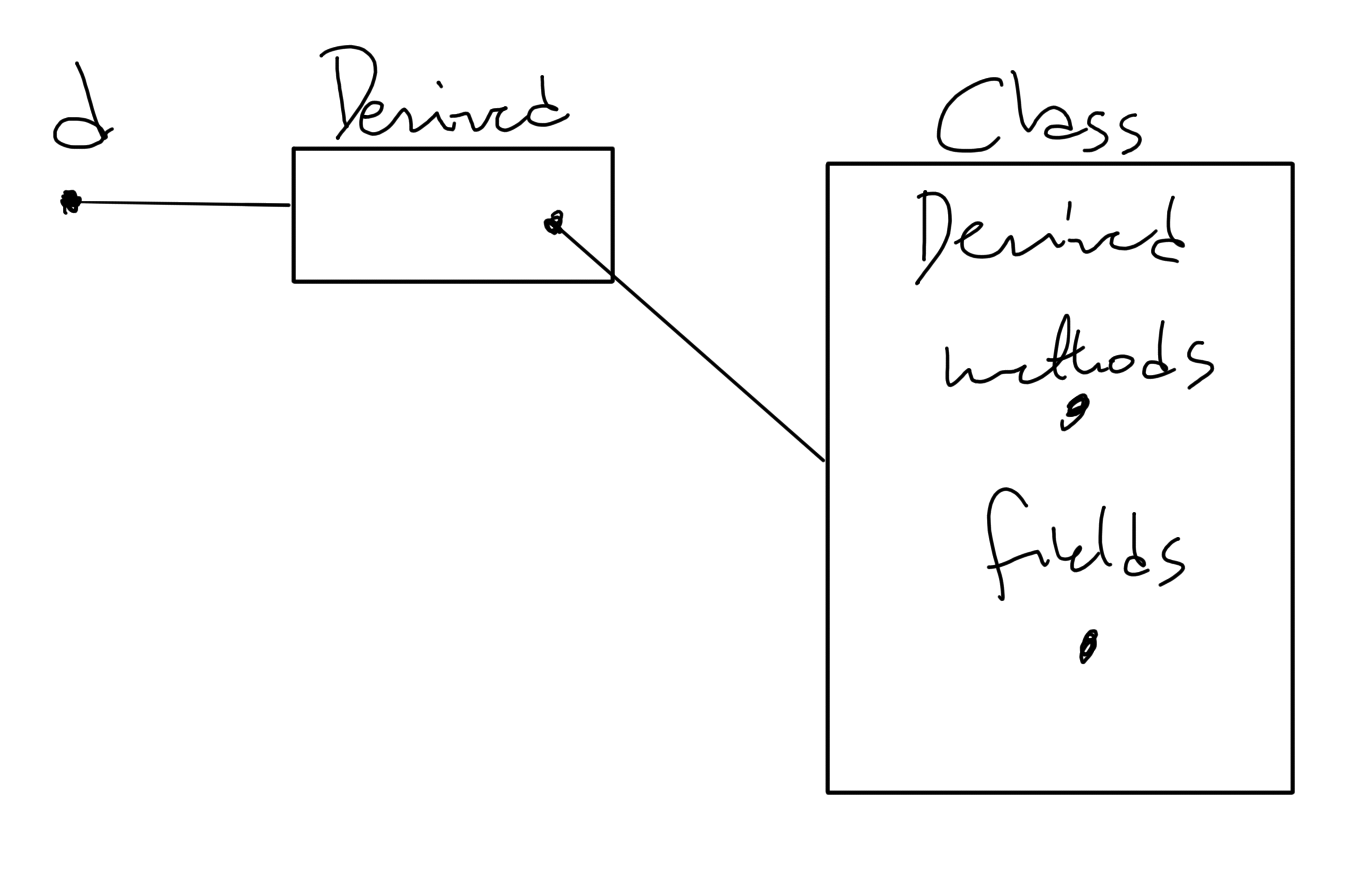
\includegraphics[ width=.6\linewidth, height=\textheight, keepaspectratio]{./pics/paintings/snippet199.png}
    \label{fig:snippet199}
\end{figure}
\clearpage

Concettualmente, all'interno di un'istanza di \texttt{X}, c'è un field di tipo
\texttt{Class}\footnote{Attenzione a non far confusione: \texttt{Class} e
\texttt{Object} sono classi. Non si può adoperare \texttt{class} per
identificatori di nessun tipo, poiché è una parola riservata (una buona
alternativa è \texttt{clazz}). È possibile, d'altronde, adoperare
l'identificatore \texttt{object} perché non è riservato dal linguaggio Java.}
dove risiede l'informazione relativa a tutti i metodi ed i field
\textbf{dichiarati}, privati o pubblici che siano. All'interno dell'oggetto
\texttt{Class} vi sono concettualmente\footnote{Osservando nel dettaglio la
classe \texttt{Class}, potrebbe esserci un maggiore dettaglio. Pertanto,
l'esistenza dei due field è soltanto un'\emph{approssimazione} del funzionamento
interno di tale classe.} dei riferimenti ad array, 

\begin{itemize}
  \item il riferimento \texttt{method} ad un array che contiene tutti e soli i
  metodi dichiarati in \texttt{X};
  \item il riferimento \texttt{field} ad un array che contiene tutti e soli i
  field dichiarati in \texttt{X}.
\end{itemize}

La classe \texttt{Derived} conterrà tutti i metodi della classe \texttt{Base}
\--- il viceversa non varrà.

Un ulteriore field contenuto in oggetti di tipo \texttt{Class} è il field
\texttt{superclass}. 

\begin{figure}[hb]
    \centering
    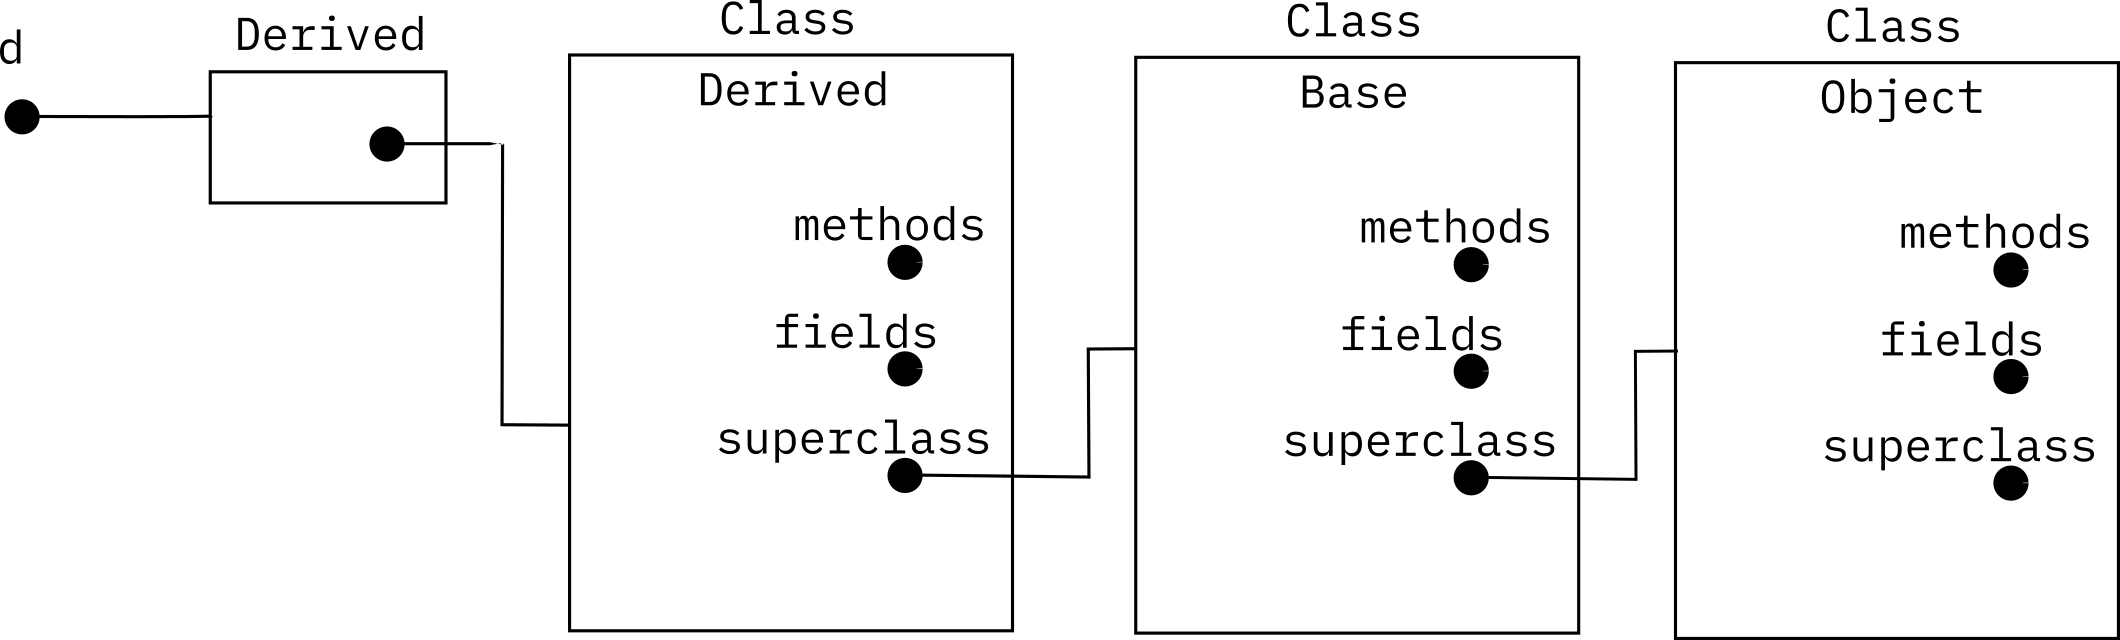
\includegraphics[ width=1\linewidth, height=\textheight, keepaspectratio]{./pics/svgs/snippet200.png}
    \caption{Riferimento alle superclassi nel caso del metodo
    \texttt{getClass()}.}
    \label{fig:snippet200}
\end{figure}

Supponendo di avere un oggetto di tipo \texttt{Derived}. In questo caso,

\begin{itemize}
  \item \texttt{methods} di \texttt{d.getClass()} contiene \texttt{doDerived};
  \item \texttt{methods} di \texttt{d.getClass().superclass} contiene
  \texttt{doBase};
  \item \texttt{methods} di \texttt{d.getClass().superclass.superclass} contiene
  \texttt{toString}, \texttt{getClass};
\end{itemize}

Questo tipo di ispezione degli oggetti è detto \textbf{reflection}.

\subsection{Esempio di polimorfismo: il metodo \texttt{println}}

Ritornando al frammento che stampa la rappresentazione testuale di un oggetto,

\begin{lstlisting}
  System.out.println(x); // -> derived.toString()

public void println(Object x) {
  if ( x == null ) {
    println("null");
  } else {
    println(x.toString());
  }
}
\end{lstlisting}

vengono effettuati numerosi passaggi concettuali. In particolare,

\begin{enumerate}
  \item Java ottiene la \texttt{Class c} dell'oggetto \texttt{x};
  \item successivamente, ottiene il field \texttt{methods} di \texttt{c};
  \item se \texttt{methods} contiene \texttt{toString()}, utilizza quel metodo
  \--- altrimenti, imposta \texttt{c} to \texttt{c.superclass}, e torna al punto
  $2$. La medesima verifica viene fatta per le superclassi.
\end{enumerate}

Nel caso peggiore, l'unico metodo ad ottenere una rappresentazione testuale è la
radice della gerarchia dell'albero dell'ereditarietà, la classe \texttt{Object}.

\subsection{I metodi della classe \texttt{Object}}

Abbiamo almeno $3$ metodi d'interesse,

\begin{itemize}
  \item \texttt{Class<?> getClass()}: returns the runtime class of this Object;
  \item \texttt{String toString()}: returns a string representation of the
  object;
  \item \texttt{equals(Object obj)}: indicates whether some other object is
      \textbf{``equal to''} this one.
\end{itemize}

Il metodo \texttt{equals} è differente dall'adoperare l'operatore \texttt{==}
\--- infatti, l'operatore binario \texttt{a == b} ha la seguente descrizione del
funzionamento:

\begin{itemize}
  \item \texttt{a} e \texttt{b} sono tipi primitivi, ma sono di tipi diversi,
  oppure primitivi e non primitivi, oppure ancora di tipi non primitivi non
  compatibili\footnote{Non compatibili significa che non c'è modo che i due
  riferimenti possano far riferimento al tipo dell'altro \--- in altre parole,
  sono in diversi rami della gerarchia.}; allora \emph{il codice non compila};
  \item \texttt{a} e \texttt{b} sono dello stesso tipo primitivo; allora viene
  valutato in \texttt{true} se e solo se \texttt{a} e \texttt{b} hanno lo stesso
  valore, altrimenti viene valutato a \texttt{false}. Esistono casi specifici
  dove l'operatore binario viene valutato correttamente anche per tipi non
  primitivi con tipi primitivi;
  \item altrimenti, viene valutato \texttt{true} se \texttt{a} e \texttt{b}
  \textbf{fanno riferimento allo stesso oggetto} o entrambi non riferiscono ad
  alcun oggetto \--- dunque se sono \texttt{null} \--- altrimenti viene valutato
  a \texttt{false}.  
\end{itemize}

\begin{lstlisting}
String s1 = "hi!";
String s2 = "hi!";
String s3 = s2;
boolean b;
b = s1 == s2; // -> false
b = s2 == s3; // -> true
b = s1.length() == s2.length(); // -> true
\end{lstlisting}

Il metodo \texttt{equals()} consente di valutare qualora due oggetti sono
``uguali''. Il suo funzionamento dipende se sia stato definito in un altro
metodo, e dunque \emph{dipende dal runtime}. Alcuni esempi,

\begin{itemize}
  \item String: "true if and only if [...] represents the same sequence of
  characters [...]"
  \item Date: "true if and only if [...] represents the same point in time, to the
  millisecond [...]"
  \item PrintStream: does not override equals(): the developers of PrintStream
  decided that the "equal to" notion of Object hold for PrintStreams
\end{itemize}

Con la classe \texttt{Object} viene poi fornita la documentazione, fornita con
il doppio intento per l'utilizzatore e per lo sviluppatore. Dalla documentazione,



\begin{quote}
\footnotesize{Indicates whether some other object is "equal to" this one.

The \texttt{equals} method implements an equivalence relation on non-null object
references:

It is \emph{reflexive}: for any non-null reference value \texttt{x},
\texttt{x.equals(x)} should return \texttt{true}.  

It is \emph{symmetric}: for any non-null reference values \texttt{x} and
\texttt{y}, \texttt{x.equals(y)} should return \texttt{true} if and only if
\texttt{y.equals(x)} returns \texttt{true}.  

It is \emph{transitive}: for any non-null reference values \texttt{x},
\texttt{y}, and \texttt{z}, if \texttt{x.equals(y)} returns \texttt{true} and
\texttt{y.equals(z)} returns \texttt{true}, then \texttt{x.equals(z)} should
return \texttt{true}.  

It is \emph{consistent}: for any non-null reference values \texttt{x} and
\texttt{y}, multiple invocations of \texttt{x.equals(y)} consistently return
\texttt{true} or consistently return \texttt{false}, provided no information
used in equals comparisons on the objects is modified.  

For any non-null reference value \texttt{x}, \texttt{x.equals(null)} should
return \texttt{false}.  

The equals method for class Object implements the most discriminating possible
equivalence relation on objects; that is, for any non-null reference values x
and y, this method returns \texttt{true} if and only if \texttt{x} and
\texttt{y} refer to the same object (\texttt{x == y} has the value
\texttt{true}).  }
\end{quote}



Dunque, il metodo \emph{equals} permette di modellare una relazione di
equivalenza fra oggetti. Esso andrebbe riscritto dallo sviluppatore, per ogni
classe che ne deve fare uso. L'implementazione deve soddisfare determinate
proprietà, enunciate sopra nella citazione alla documentazione \--- nella
classe \texttt{Object}, tali linee guida sono implementate facendo sì che due
oggetti risultino uguali se lo sono nel senso dell'operatore binario
\texttt{==}, cioé se due riferimenti fanno riferimento allo stesso oggetto.
Solitamente, il metodo \texttt{equals} viene riscritto soltanto per classi
aventi field; in tal caso, infatti, i field permettono di stabilire le
relazioni di equivalenza a seconda dei casi.

In altre parole, nella classe \texttt{Object} si avrà qualcosa del tipo

\begin{lstlisting}
  public class Object {
    /* ... */
    public boolean equals(Object other) {
      if (other == null) {
        return false;
      }
      return this == other;
    }
  }
\end{lstlisting}

dove \texttt{this} non può mai essere \texttt{null}. I requisiti per l'override
del metodo sono i seguenti:
\begin{itemize} 
  \item mantenere la medesima signature, 

  \begin{lstlisting}
    public boolean equals(Object other)
  \end{lstlisting} 

  caso gestito dal compilatore;

  \item implementare il concetto di \textbf{relazione d'equivalenza} per il caso
  specifico \--- non gestito dal compilatore;
  \item proprietà di \emph{riflessività}, \emph{simmetria}, \emph{transitività},
  \emph{consistenza}, gestione del caso \texttt{null} \--- non gestito dal
  compilatore.
\end{itemize}

L'implementazione del concetto di relazione d'equivalenza dipende largamente dal
contesto. Ad esempio, il concetto stesso di \emph{persona} potrebbe variare a
seconda del luogo: in un Ospedale, a livello scientifico, a livello di numero di
matricola, e così via, con i casi più disparati che dipendono da \emph{come il
mondo reale è modellato}. Una possibile modellazione è la seguente,

\begin{lstlisting}
public class Person {
  private String firstName;
  private String lastName;
  private Date birthDate;
}
\end{lstlisting}

dove ogni persona è univocamente modellata da $3$ campi. Allora il metodo
\texttt{equals} potrebbe semplicemente comparare i campi all'interno della
classe. Tuttavia, questo potrebbe non andare bene a seconda dei contesti,
pensiamo al caso ad esempio di una persona che cambi nome, oppure di due persone
aventi stesso nome, cognome, e medesima data di nascita per pura coincidenza.
La realtà viene modellata dallo sviluppatore: è dunque sua sola responsabilità
la scelta di come viene poi implementata la relazione di equivalenza, a seconda
del contesto e delle necessità.

Una modellazione differente è la seguente, dove viene aggiunto un campo
contenente il codice fiscale,

\begin{lstlisting}
public class Person {
  private String firstName;
  private String lastName;
  private Date birthDate;
  private String fiscalCode;
}
\end{lstlisting}

In tal caso, il metodo \texttt{equals} potrebbe semplicemente richiedere che due
persone abbiano lo stesso codice fiscale per essere considerate la stessa
persona. Tutto ciò viene introdotto dallo sviluppatore, tramite la
\textbf{conoscenza di dominio}.

Supponiamo ora di implementare la prima versione,

\begin{lstlisting}
  public class Person {
    private String firstName;
    private String lastName;
    private Date birthDate;
    public boolean equals(Object other) {
      if (other == null) {
        return false;
      }
      if (!(other instanceof Person)) {
        return false;
      }
      if (!firstName.equals(((Person) other).firstName)) {
        return false;
      }
      if (!lastName.equals(((Person) other).lastName)) {
        return false;
      }
      if (!birthDate.equals(((Person) other).birthDate)) {
        return false;
      }
      return true;
    }
  }
\end{lstlisting}

Si osservi che sono stati effettuati dei \emph{downcast} per l'oggetto
\texttt{other}, di modo da farlo funzionare anche per oggetti di tipo più basso
in gerarchia.

Implementando la seconda possibilità, si ottiene

\begin{lstlisting}
  public class Person {
    private String firstName;
    private String lastName;
    private Date birthDate;
    private String fiscalCode;
    public boolean equals(Object other) {
      if (other == null) {
        return false;
      }
      if (!(other instanceof Person)) {
        return false;
      }
      if (!fiscalCode.equals(((Person) other).fiscalCode)) {
        return false;
      }
      return true;
    }
  }
\end{lstlisting}

\subsection{La classe \texttt{Objects}}

\texttt{Objects} è una classe \textbf{di utilità}\footnote{Trattasi di una
classe che modella un componente capace di fare operazioni, ma non dotato di
uno stato. Si differiscono dal nome (con una \textbf{s}) e dalla presenza di
metodi statici. Tipicamente, il costruttore non è public.}, static per scelta.
Essa fornisce il metodo \texttt{equals}. Dalla documentazione,


\begin{quote}
    \footnotesize{This class consists of static utility methods for operating on objects, or
    checking certain conditions before operation.

    \texttt{static int 	checkIndex(int index, int length)} 	Checks if the index is within the bounds of the range from 0 (inclusive) to length (exclusive).

    \texttt{static boolean 	deepEquals(Object a, Object b)} 	Returns true if the arguments are deeply equal to each other and false otherwise.

    \texttt{static boolean 	equals(Object a, Object b)} 	Returns true if the arguments are equal to each other and false otherwise.

\texttt{static boolean 	isNull(Object obj)} 	Returns true if the provided reference is null otherwise returns false.}
\end{quote}


Il metodo \texttt{deepEquals} è simile ad \texttt{equals}, ma funziona anche
con gli array, facendo il confronto elemento per elemento nel vettore. Un altro
esempio di classi di utilità forniti all'interno del JDK è la classe
\texttt{Arrays}, che fornisce \texttt{sort()}, \texttt{fill()}, e così via.

\subsection{Differenze fra \texttt{instanceof} e \texttt{getClass()}}

In apparenza, si somigliano. Tuttavia, 

\begin{itemize}
    \item \texttt{a instanceof B} vero se e solo se \texttt{a} potrebbe essere
        legittimamente referenziato da un riferimento \texttt{b} ad oggetti di
        tipo \texttt{b};
    \item \texttt{a.getClass() == b.getClass()} vero se e solo se al runtime la
        classe di oggetti referenziati da \texttt{a} è esattamente la stessa
        (\texttt{==}) della classe di oggetti referenziata da \texttt{b};
    \item \texttt{a.getClass() == B.class} identica alla seconda \---
        \texttt{class} è approssimativamente un field statico definito
        implicitamente in ogni classe, che fa riferimento all'oggetto che
        rappresenta la classe (in questo caso, la classe \texttt{B}). Si usa
        qualora volessimo confrontare una classe con un oggetto, o viceversa.
\end{itemize}


\begin{figure}[h]
    \centering
    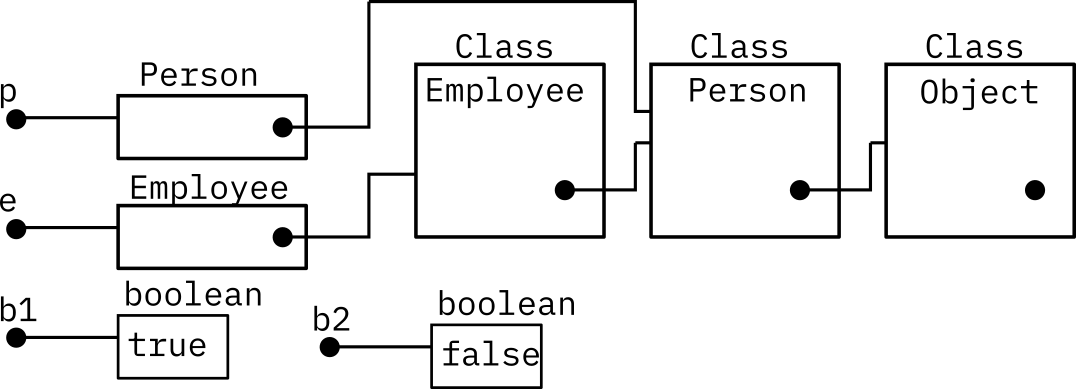
\includegraphics[ width=1.0\linewidth, height=\textheight, keepaspectratio]{./pics/png/snippet219.png}
    \caption{Situazione in memoria con l'utilizzo di \texttt{instanceof} e
    \texttt{getClass()}.}
    \label{fig:snippet219}
\end{figure}



Supponiamo di avere lo snippet seguente, con diagramma oggetti-riferimenti
mostrato in Figura~\ref{fig:snippet219}.

\begin{lstlisting}
public class Person { /* ... */ }

public class Employee extends Person { /* ... */ }

Person p = new Person( /* ... */ );
Employee e = new Employee( /* ... */ );
boolean b1 = e instanceof Person; // -> true
boolean b2 = p.getClass() == e.getClass(); // -> false
\end{lstlisting}

La scelta dei due dipende esclusivamente dalla modellazione adoperata.
Supponiamo di voler paragonare l'impiegato alla persona \--- in questo caso, si
potrebbe decidere che per una tale eguaglianza che andiamo a modellare
l'uguaglianza sia verificata oppure no.

Si vuole modellare i \emph{multiset} e le \emph{sequenze}. Matematicamente,

\begin{itemize}
    \item un \emph{multiset} o \emph{bag} è un insieme di elementi in cui ogni elemento può
        apparire da $0$ a più volte. Precisamente, $$\mathcal X = \mathcal M
        (\mathbb{Z}) = \{f:\mathbb{Z} \rightarrow \mathbb{N}\}.$$ L'equivalenza
        di $x_1$ ed $x_2$ considera sia la lunghezza (stesso numero di
        elementi) che gli elementi (ogni elemento compare lo stesso numero di
        volte). Essa potrebbe essere modellata da 
        

\begin{lstlisting}
public class BagOfInts {
  private int[] values;
}
\end{lstlisting}
    \item un \emph{insieme delle sequenze} di interi è un $$\mathcal X = \bigcup
        _{i\in\mathbb{N}}\mathbb{Z}^i.$$ La relazione di equivalenza stavolta
        considera, per due elementi $x_1$, $x_2$, anche l'\emph{ordine} degli
        elementi presenti. In questo caso, potrebbe essere modellata con

\begin{lstlisting}
public class SequenceOfInts {
  private int[] values;
}
\end{lstlisting}
\end{itemize}

Osserviamo che la modellazione, almeno in questo caso, è identica dal punto di
vista del compilatore, poiché il codice è diverso \--- tuttavia, il resto dei
dettagli sarà diverso (a partire dal nome). La differenza fra i due modelli
dovrebbe essere catturata dal \textbf{nome} del tipo.

\section{Ereditarietà multipla in Java?}

Si prenda in considerazione l'idea di voler modellare l'universo dei veicoli
con il linguaggio Java. Si potrebbe voler effettuare una modellazione del tipo
seguente, basandoci sostanzialmente sulle caratteristiche dei veicoli (hanno un
motore, hanno ruote, sono veicoli nautici, e così via):

\begin{lstlisting}
public class Vehicle { /* ... */ }

public class MotorVehicle extends Vehicle {
  public void startEngine() { /* ... */ }
}

public class Motorboat extends MotorVehicle {
  public void startEngine() { System.out.println("bl bl bl"); }
  public void turnPropeller() { /* ... */ }
}

public class Car extends MotorVehicle {
  public void startEngine() { System.out.println("brum brum"); }
  public void turnWheels() { /* ... */ }
}
\end{lstlisting}

Capita però che ci siano casi in cui la relazione fra le entità non è ad
albero, e parrebbe avere un senso realizzare una qualche sorta di \emph{ereditarietà
multipla,} del tipo \emph{AmphibiousVehicle} che estenderebbe sia le \emph{Motorboat} che le \emph{Car}:

\begin{lstlisting}
public class AmphibiousVehicle extends Motorboat, Car { // NOOOO!
  public void doAmphibiousFancyThings() { /* ... */ }
}
\end{lstlisting}

ciononostante, questo codice \textbf{non compila}, poiché l'ereditarietà
multipla in Java non è implementata. Come effettuiamo dunque la modellazione di
tale entità?

Supponiamo infatti di avere un veicolo anfibio istanziato come nel seguente
frammento,

\begin{lstlisting}
public class AmphibiousVehicle extends Motorboat, Car { // NOOOO!
  public void doAmphibiousFancyThings() { /* ... */ }
}

AmphibiousVehicle fiat6640 = new AmphibiousVehicle();
fiat6640.startEngine();
\end{lstlisting}

all'esecuzione di \texttt{startEngine()} che cosa succede? Quale dei due metodi
viene eseguito, quello ridefinito nella classe \texttt{Motorboat} o quello
ridefinito nella classe \texttt{Car}? La sintassi Java non consente di
specificare allo sviluppatore quale metodo adoperare \--- una scelta precisa
degli sviluppatori Java, allo scopo di non caricare lo sviluppatore di troppe
responsabilità e, di fatto, sacrificando l'espressività.

Supponiamo ancora che gli sviluppatori di Java abbiano consentito l'ereditarietà \textbf{solo} nel caso in cui le classi padri sono \textbf{disgiunte}, come nel frammento seguente

\begin{lstlisting}
public class A { public void doA() { /*...*/ } }

public class B { public void doB() { /*...*/ } }

public class C extends A, B { public void doC() { /*...*/ } }
\end{lstlisting}

Anche in questo caso vi sono problemi \--- cosa accadrebbe infatti se gli
sviluppatori della classe \texttt{A} e della classe \texttt{B} decidessero di
aggiungere entrambi la ridefinizione del metodo \texttt{toString()}? In tal
caso la condizione non sarebbe più verificata.

\subsection{L'espressione \texttt{switch}}

L'espressione \texttt{switch} viene introdotta tramite il seguente esempio,

\begin{lstlisting}
public static RegularPolygon createPolygon(
    int nOfSides,
    double sideLength
) {
  return switch (nOfSides) {
    case 3 -> new Triangle(sideLength);
    case 4 -> new Square(sideLength);
    case 5 -> new Pentagon(sideLength);
    default -> null;
  };
}
\end{lstlisting}

L'espressione \texttt{switch} viene considerata valida dal compilatore
solamente nel caso in cui \textbf{l'intero spazio delle possibilità è gestito dal
costrutto}. Questo equivale a specificare ogni singola possibilità del valore
nell'argomento dello switch \-- poiché è impossibile coprire ogni caso
personalmente, si adopera la keyword \texttt{default}, che consente di
``catturare'' tutti i casi possibili. 
Il costrutto \texttt{switch} si sposa bene nel caso vi siano pochi valori
d'interesse, con range piccoli di valori da specificare.

Un costrutto \texttt{switch} non ammette casi \texttt{boolean}, poiché
eccessivamente banali.

\section{Riassunto del capitolo}

\begin{description}
    \item[Legame fra classe estesa e classe che estende] Esiste un legame fra
        la classe estesa e la classe derivata -- in particolare, tutto il
        codice che funziona per la classe estesa funzionerà anche per la classe
        derivata: infatti, la classe derivata avrà \textbf{almeno} i metodi
        della classe che estende. Perciò, si possono assegnare tipi differenti
        purché il tipo assegnato abbia i metodi della classe base (cioè, sia
        dello stesso tipo o derivi da essa). Dunque, mediante l'ereditarietà
        siamo in grado di riutilizzare codice ma aggiungendo nuove
        funzionalità, definendo gerarchie concettuali.
    \item[Riduzione della visibilità] Non ammessa in Java.
    \item[Polimorfismo] Il \textbf{polimorfismo} è una proprietà dinamica del
        linguaggio per cui viene realizzata l'ereditarietà, con il codice che
        esibisce comportamenti differenti a seconda del tipo effettivo
        dell'oggetto che viene manipolato al momento dell'esecuzione.
    \item[Conseguenze del polimorfismo] al runtime, uno stesso metodo può
        essere eseguito con la classe base o con la classe derivata, a seconda
        del tipo -- è una conseguenza dinamica del polimorfismo. Pertanto è
        possibile che un oggetto base sia inizializzato con un costruttore di
        classe derivata -- in tale circostanza, verranno eseguiti metodi della
        classe derivata. Non è invece possibile il contrario, poiché potrebbero
        mancare metodi alla classe base.
    \item[Downcasting] Poiché è impossibile far sì che una classe derivata sia
        inizializzata a partire da un costruttore della classe base, la
        sintassi fra parentesi tonde detta \textbf{downcasting} è l'unico modo
        per forzare la compilazione. La sintassi cambia il tipo di riferimento
        downcast, funziona soltanto se la classe derivata deriva direttamente o
        indirettamente da quella base. Tuttavia, dinamicamente, la JVM
        provvederà a verificare l'esistenza dei metodi: qualora non fossero
        garantiti, non funzionerebbe e si bloccherebbe tutto.
    \item[\texttt{instanceof}] Operatore binario per controllare il tipo di un
        oggetto al runtime. Valuta come un \texttt{boolean} -- \texttt{a
        instanceof b} restituisce \texttt{true} se e solo se l'oggetto a cui fa
        riferimento \texttt{a} può essere legittimamente riferito dal
        riferimento \texttt{b} ad oggetti di classe \texttt{B}.
        \texttt{instanceof} realizza il cosiddetto \textbf{Pattern matching}.
    \item[\texttt{toString()}] Metodo che restituisce la descrizione testuale
        di un oggetto. Genericamente esso appartiene ad \texttt{Object};
        dunque, ciascun oggetto di qualsivoglia classe ne sarà dotato.
    \item[Il field \texttt{Class}] Field ereditato dalla classe
        \texttt{Object}, presente in qualunque classe, indicato con la lettera
        maiuscola, con modificatori \texttt{static} e \texttt{private}. Per
        accedervi si utilizza il metodo \texttt{getClass()}, anch'esso della
        classe \texttt{Object}. Tale metodo restituisce, al runtime
        (polimorfismo), il \textbf{tipo} della classe dell'oggetto. Tutti gli
        oggetti di una determinata classe avranno un riferimento al singolo
        oggetto della classe \texttt{Class}.
    \item[L'oggetto \texttt{Class}] L'oggetto \texttt{Class} contiene le
        informazioni relative a tutti i metodi e field \textbf{dichiarati},
        privati o pubblici che siano -- sotto forma di array \texttt{method} ed
        array \texttt{field}. Un oggetto di classe \texttt{Class} ``Derived''
        conterrà solo ed esclusivamente i metodi dichiarati in Derived, non i
        metodi dichiarati in Base -- l'oggetto relativo di classe
        \texttt{Class} ``Base'' conterrà a sua volta tutti e soli i metodi
        dichiarati in Base (lo stesso vale, naturalmente, per i field). Esiste
        anche un riferimento \texttt{superclass}, che contiene il riferimento
        all'oggetto di classe \texttt{Class} che è superclasse della classe che
        si sta considerando. Concettualmente e un po' più nella pratica, è così
        che si verificano i controlli dell'ereditarietà e del polimorfismo.
    \item[Passaggio alla superclasse] Si verifica qualora il compilatore o la
        JVM non dovesse trovare nell'array ``concettuale'' \texttt{methods}; in
        tal caso, si imposta \texttt{c = c.superclass} e si ripete la verifica
        fino alla superclasse \texttt{Object}.
    \item[Il metodo \texttt{equals()}] Metodo che indica se un oggetto è
        ``equal to'' ad un altro. La differenza con l'operatore binario di
        uguaglianza è che quest'ultimo,
        \begin{itemize}
            \item non compila se sono tipi primitivi diversi, non compatibili, o tipi
                primitivi non compatibili (non sullo stesso ramo della gerarchia), o
                tipo primitivo e non primitivo;
            \item per tipi primitivi, è \texttt{true} soltanto se i due oggetti di tipo
                primitivo hanno lo stesso valore; altrimenti, è \texttt{false}.
                Esistono sporadici casi in cui l'operatore binario viene valutato anche
                fra un tipo primitivo e un tipo non primitivo.
            \item per tipi non primitivi, è \texttt{true} se i due riferimenti fanno
                riferimento allo stesso oggetto, è \texttt{false} diversamente. Viene
                valutato \texttt{true} anche se ambedue riferiscono a \texttt{null}.
        \end{itemize}
        mentre invece il metodo \texttt{equals()} consente di definire, più
        precisamente, la maniera in cui due oggetti di tipo non primitivo
        debbano essere ``uguali''. Esso andrebbe ridefinito, dunque il suo
        funzionamento dipende dal runtime.
    \item[Proprietà del metodo \texttt{equals()}] Il metodo \texttt{equals()}
        deve godere di determinate proprietà -- \textbf{riflessività}
        (\texttt{x.equals(x)} restituisce \texttt{true} se \texttt{x != null}),
        \textbf{simmetria} (\texttt{x.equals(y) == y.equals(x)}),
        \textbf{transitività} (\texttt{x.equals(y) == y.equals(z) == true =>
        x.equals(z) == true} e viceversa), \textbf{consistenza} (a meno di
        \texttt{null}, il risultato non deve dipendere dal tempo),
        \textbf{gestione del null} (\texttt{x.equals(null) == false} se
        \texttt{x != null}). Il metodo \texttt{equals()} della classe
        \texttt{Object} implementa \texttt{a == b} per tipi non primitivi.
    \item[La classe di utilità \texttt{Object}] La classe di utilità (classe
        che modella un componente capace di fare operazioni, ma non dotato di
        uno stato -- si differisce dal nome per via del plurale, tipicamente
        adoperato, e dalla presenza di metodi \texttt{static} e costruttore
        privato) \texttt{Objects} fornisce i metodi \texttt{isNull()}
        (restituisce \texttt{true} se è il riferimento all'oggetto fa
        riferimento a \texttt{null}) e due metodi per comparare oggetti
        \texttt{equals()} e \texttt{deepEquals()} -- il secondo è simile al
        primo, tuttavia esso è in grado di verificare l'uguaglianza fra
        vettori di oggetti.
    \item[Differenza fra \texttt{instanceof} e \texttt{getClass()}] La
        differenza, in breve, è che facendo \texttt{a.getClass() ==
        b.getClass()} si ottiene \texttt{true} esclusivamente nel caso in cui
        le due classi siano \textbf{esattamente} le stesse.
    \item[Ereditarietà multipla] L'ereditarietà multipla non è ammessa in Java.
\end{description}


\chapter{Parametri, visibilità degli identificatori e memoria}
\section{Passaggio dei parametri}

Nel seguente frammento di codice, non risulta subito evidente se i parametri
sono passati \textbf{per valore} o \textbf{per riferimento}, in particolare non
è ben chiaro se il parametro passato alla funzione subisca modifiche visibili
dall'esterno oppure non ne subisca. Infatti, supponendo di modellare una
persona che può cambiare nome,

\begin{lstlisting}
// The class models person that can change its name
public class Person {
  private String name;
  public Person(String name) { this.name = name; }
  public String getName(){ return name; } //getter
  public void setName(String name){ this.name = name; } //setter
}

public void modify(Person p) {
  p.setName(p.getName().toUpperCase());
  //no return!
  //does p get modified?
}

Person eric = new Person("Eric");
modify(eric);
System.out.println(eric.getName());
\end{lstlisting}

La funzione \texttt{public void modify(Person p)} \textbf{non presenta valore
di return}. Dunque, lo stato interno (il nome) viene modificato?

Il passaggio \textbf{by value} prevede che la funzione chiamata riceva
\textbf{una copia} dell'oggetto \---- viceversa, il passaggio \textbf{by
reference} prevede che la funzione chiamata riceva, invece, \textbf{l'oggetto
stesso}, o meglio una \textbf{copia del riferimento} dell'oggetto. I tipi
primitivi sono passati sempre \emph{by value}, mentre i tipi non primitivi sono
sempre passati \emph{by reference}. Il tipo del passaggio, pertanto, è una fra
le differenze cruciali che i tipi non primitivi presentano rispetto ai tipi
primitivi.

Poiché \texttt{Person p} è un tipo non primitivo, viene passata una copia per
riferimento. La modifica perciò avrà un effetto visibile anche successivamente.
Per esempio,

\begin{lstlisting}
public void modify(Person p) { // B
  p.setName(p.getName().toUpperCase());
}

Person eric = new Person("Eric"); // A
modify(eric); // C
\end{lstlisting}

La situazione in memoria dei tre casi è la seguente: 
\begin{itemize}
    \item nel punto del codice A esiste soltanto un riferimento all'oggetto di
        tipo \texttt{Person} di nome \texttt{eric};
    \item nel punto B avremo che esiste un ulteriore riferimento, \texttt{p},
        che riferisce anch'esso all'oggetto di tipo \texttt{Person}: una copia del
        riferimento \texttt{eric}. Nel contesto del metodo \texttt{modify}, non
        esiste il riferimento \texttt{eric};
    \item nel punto C infine, il field interno del nome farà riferimento alla
        nuova stringa, di contenuto \texttt{"ERIC"}. La situazione finale è che
        il cambiamento è visibile, e l'oggetto di tipo \texttt{Person} vede il
        suo field fare riferimento ad una nuova stringa, non dunque più alla
        stringa con contenuto \texttt{"Eric"}.
\end{itemize}

Nel caso del passaggio di tipi primitivi, la situazione è diversa. Prendiamo ad
esempio il frammento seguente,

\begin{lstlisting}
public void uselesslyModify(int n) { // B
  n = 18;
}

int age = 42;         // A
uselesslyModify(age); // C
\end{lstlisting}

non si produrranno effetti visibili, poiché useless modify riceve soltanto
\emph{una copia} del tipo primitivo, non il riferimento all'oggetto
\texttt{int}. Dunque, il tipo primitivo esterno viene in qualche maniera
``protetto'', poiché non viene passato direttamente, ma viene passata
esclusivamente una sua copia; in questo caso, il metodo
\texttt{uselesslyModify()} non produce un cambiamento.

\section{La parola chiave \texttt{final}}

Il modificatore \texttt{final} è una keyword applicabile a classi, metodi,
field e variabili, di tipo \textbf{statico}, cioè che i suoi effetti sono
prodotti \emph{esclusivamente in tempo di compilazione} \-- al runtime è come
se non esistesse; l'effetto al runtime è dunque esclusivamente implicito (se
non compila, non esegue\dots). La parola chiave \texttt{final} ha un effetto
diverso a seconda del tipo di definizione, distinguendo fra metodi e classi,
field e variabili.

L'effetto su una \textbf{classe} è che essa \textbf{non può essere estesa}. Una
classe dichiarata con modificatore \texttt{final} e successivamente estesa
vedrà un errore in fase di compilazione.

L'effetto su un \textbf{metodo} è che esso \textbf{non può essere ridefinito}.
Estendendo una classe non \texttt{final} con un metodo \texttt{final} e
provando a ridefinire tale metodo, viene prodotto un errore in fase di
compilazione.

Con il modificatore \texttt{final} su classi e metodi, nella sostanza, viene
limitata l'ereditarietà.

L'effetto su un \textbf{field} e \textbf{variabili} è che esse \textbf{non
possono essere assegnate più di una volta}; in altre parole, non può cambiare
il loro valore, sono \emph{costanti}. Forzando il cambio di valore viene
prodotto un errore in fase di compilazione.

Entrambi i seguenti frammenti di codice non compilano per le ragioni di cui
sopra,

\begin{lstlisting}
public class Greeter {
  private final String msg = "Hi!";
  public void update(String msg) {
    this.msg = msg;
  }
}

/////
public class Greeter {
  public void update(final int n) {
    n = 18;
  }
  public void doThings() {
    final String s = "hi!";
    s = "hello";
  }
}
\end{lstlisting}

Le ragioni principali per l'adozione del modificatore \texttt{final} sono
varie; principalmente, si adotta per la modellazione. Il modificatore
\texttt{final} \textbf{modella entità che non possono cambiare}. Domandiamo
perciò al compilatore di ricordarci che la nostra modellazione è quella di una
costante \-- non può e non deve essere cambiata. Questa funzionalità serve sia
a noi stessi, che agli altri sviluppatori.

Nella pratica, vi sono 3 casi d'uso:
\begin{itemize}
    \item definire delle \textbf{costanti}, specialmente nel caso dei field;
    \item limitare la \textbf{riusabilità}, caso molto raro \-- in linea di
        principio, potrebbero esistere dei casi in cui sia desiderabile che dei
        metodi non \texttt{private} mantengano un accesso regolato allo stato
        interno dell'oggetto (ad esempio, per i \textbf{getter} ed i
        \textbf{setter}). Tali metodi andrebbero impostati come \texttt{final},
        di modo che lo stato sia modificabile solo ed esclusivamente in maniera
        regolata;
    \item rimarcare l'\textbf{immutabilità}, caso ancor più raro. La sintassi
        del linguaggio può consentire la mutazione di alcune costanti, non
        ovvie, anche nel caso in cui non sia desiderabile.
\end{itemize}

Si possono definire costanti sia per oggetti, che per le classi \-- in questo
ultimo caso, il valore è uguale per tutte le istanze di tale classe.

Una costante per l'oggetto (object-wise) è un field \textbf{immutabile} che può avere valori
differenti per i diversi oggetti, ma che una volta fissato non può cambiare. Di
solito, per tali field viene deciso un modificatore \texttt{final private}.

Di contro, una costante per la classe (class-wise) è un field
\textbf{globale} e \textbf{immutabile}, cioè un placeholder per un valore
codificato e costante per tutte le istanze. Esse sono dichiarate mediante i
modificatori \texttt{final static}, con il modificatore \texttt{static} che la
rende di fatto globale.

L'utilizzo di uno o dell'altro tipo di costanti è una prerogativa esclusiva
dello sviluppatore. Un esempio di ciò è la classe \texttt{Person} definita nel
seguente frammento,

\begin{lstlisting}
public class Person {
  private String firstName;
  private String lastName;
  private final Date birthDate;
  private final String fiscalCode;
  public Person(Date birthDate, String fiscalCode) {
    this.birthDate = birthDate;
    this.fiscalCode = fiscalCode;
  }
}
\end{lstlisting}

dove i field \texttt{birthDate} e \texttt{fiscalCode} sono considerati
\textbf{immutabili} per una singola istanza dell'oggetto (object-wise). Ogni
costruttore \textbf{deve} necessariamente inizializzare i field immutabili \--
pena l'invalidità in fase di compilazione. Secondo questa modellazione, per
definire una persona bisogna almeno definire codice fiscale e data di nascita.
Una conseguenza di ciò è che ambedue i field immutabili non possono essere
successivamente modificati.

Un esempio di class-wise constant è invece esplicitato nel frammento seguente,

\begin{lstlisting}
public class Doc extends Person {
  private final static String TITLE_PREFIX = "Dr.";
  public String getFullName() {
    return TITLE_PREFIX + " " + firstName + " " + lastName;
  };
}
\end{lstlisting}

dove viene specificato che \textbf{ogni} istanza della classe \texttt{Doc}
contiene il prefisso \texttt{"Dr."}. Poiché si tratta di una costante
\textbf{globale ed immutabile}, viene adoperata una nuova naming convention:
\textbf{tutto maiuscolo e parole separate mediante underscore}.

Un esempio di ciò è la costante globale \texttt{Math.PI}, con modificatore
\texttt{public final static}.

Per rimarcare l'immutabilità, si adopera l'identificatore \texttt{final} negli
argomenti di un metodo:

\begin{lstlisting}
public void update(final int n) { // remarks immutability, no effect outside
  /* ... */
}
\end{lstlisting}

L'identificatore \texttt{final} diventa dunque un monito per lo sviluppatore a
ricordare che il valore di \texttt{n} non deve cambiare, e non ha effetto al di
fuori. In realtà, essendo un tipo primitivo sappiamo già che il suo valore non
potrebbe ugualmente cambiare; il modificatore assume dunque la funzione di
monito, ed andrebbe messo per ogni tipo primitivo.

Per quanto riguarda i tipi non primitivi passati per argomento, è utile
definire ugualmente con \texttt{final}: sarebbe altrimenti possibile
\textbf{riassegnare il riferimento}, impedendo di cambiare oggetto al quale
l'argomento si riferisce\footnote{Difatti, il modificatore \texttt{final} ha
effetto \textbf{sul riferimento} dichiarato, non sull'oggetto a cui
riferisce tale riferimento.}. In altre parole, se \texttt{p} fosse riassegnato,
le successive modifiche avrebbero effetto su un altro oggetto, non sull'oggetto
che dovrebbe essere modificato.

\begin{lstlisting}
// Do not change what p refers to!
public void capitalizeName(final Person p) {
  p.setName(
    p.getName().substring(0, 1).toUpperCase() +
    p.getName().substring(1).toLowerCase()
  );
}
\end{lstlisting}

Nel seguente frammento di codice, viene inizializzato un riferimento ad un
vettore di persone, e viene fatta un'iterazione. Con il \texttt{for each} viene
adoperata una variabile d'iterazione \texttt{final}:

\begin{lstlisting}
Person[] teachers = new Person[] {alberto, eric};
for (final Person teacher : teachers) {
  capitalizeName(teacher);
}
\end{lstlisting}

rimarcando che all'interno del ciclo \texttt{for} non vi è alcuna ragione per
riassegnare il riferimento \texttt{teacher}. Supponiamo tuttavia il seguente
frammento,

\begin{lstlisting}
Person spareTeacher = new Person(/* ... */);
Person[] teachers = new Person[] {alberto, eric};
for (Person teacher : teachers) {
  if (teacher.isIll()) { // A
    teacher = spareTeacher;
  } // B
}
\end{lstlisting}

compila, ma non fa ciò che si immagina. Durante la prima iterazione (punto A),
\texttt{teacher} viene riferito a riferire ciò che riferisce il primo elemento
dell'array \texttt{teachers}: \texttt{alberto} (fra l'altro, non malato).
Tuttavia, durante la seconda esecuzione, \texttt{eric} è malato e viene
cambiato ciò a cui \texttt{teacher} riferisce, cioè lo stesso oggetto a cui
riferisce \texttt{spareTeacher}. Tuttavia, non cambia il contenuto di
\texttt{teachers[1]}! Ciò è accaduto perché abbiamo soltanto cambiato ciò che
il riferimento riferiva, non un field di un array: sarebbe stato giusto
riassegnare il riferimento contenuto in \texttt{teachers[1]}. Un modo per
accorgersi di ciò è definire il ciclo in questa maniera,

\begin{lstlisting}
Person spareTeacher = new Person(/* ... */);
Person[] teachers = new Person[] {alberto, eric};
for (final Person teacher : teachers) {
  if (teacher.isIll()) { // A
    teacher = spareTeacher; // irrelevant to change teacher reference
  } // B
}
\end{lstlisting}

Come regola quasi generale, i \texttt{for each} vogliono vedere un modificatore
\texttt{final} nella variabile d'iterazione.

\section{Lo scope e il lifetime}

Lo \textbf{scope} è una proprietà statica degli identificatori che esplicita in
quale porzione di codice l'identificatore può essere usato \-- in altre parole,
menzionare un identificatore fuori dalla porzione di codice dal quale risulta
``visibile'' produrrà un errore in fase di compilazione. Si tratta di una
proprietà \textbf{statica} degli identificatori.

Il \textbf{tempo di vita (lifetime)} è l'intervallo di tempo entro il quale un
oggetto o un riferimento \emph{esiste}. È una proprietà \textbf{dinamica} degli
identificatori e degli oggetti.

In generale, i due concetti sono propri di altri linguaggi di programmazione,
tuttavia il loro utilizzo pratico e il loro significato variano di molto in
base al linguaggio. Inoltre, in Java anche il tipo di oggetto influenza il
lifetime di tale entità.

\subsection{Scope per le variabili}

In Java, lo scope dei riferimenti dichiarati nella signature di un metodo è
\textbf{tutto e solo il metodo}. In altre parole, ciò che è dichiarato
all'interno della signature è visibile lungo l'intero metodo dove è dichiarato.

I riferimenti dichiarati nel codice, cioè per le \emph{variabili locali}, sono
visibili \textbf{dal momento della dichiarazione sino alla fine del blocco ove
sono state dichiarate}. Dunque sono visibili nella sequenza di statement
racchiusi fra parentesi graffe, cioè all'interno dei blocchi.

Un esempio di ciò è il frammento successivo,


\begin{lstlisting}
public String capitalize(final String string) {
  String capitalized = "";
  for (final String token : string.split(" ")) {
    String head = token.substring(0, 1);
    String remaining = token.substring(1);
    capitalized = capitalized
      + head.toUpperCase() + remaining.toLowerCase() + " ";
  }
  return capitalized;
}
\end{lstlisting}

e si tratta di un metodo che \emph{capitalizza} una stringa. Il valore di
ritorno è una stringa nuova, poiché esse sono immutabili. Il metodo ha la
funzionalità di rendere la prima lettera di ogni parola come maiuscola. Vi sono
cinque differenti identificatori:
\begin{itemize}
    \item \texttt{string} \-- visibile all'interno dell'intero metodo, poiché è
        stato dichiarato direttamente nella signature;
    \item \texttt{capitalized} \-- dalla riga 2 alla riga 10;
    \item \texttt{token} \-- dalla riga 3 alla riga 8;
    \item \texttt{head} \-- dalla riga 4 alla riga 8;
    \item \texttt{remaining} \-- dalla riga 5 alla riga 8.
\end{itemize}

Vi sono tuttavia 5 possibili migliorie al frammento:
\begin{enumerate}
    \item il metodo potrebbe essere \texttt{static};
    \item il metodo aggiunge un \emph{trailing space} alla fine della stringa;
    \item \texttt{head} e \texttt{remaining} potrebbero vedere aggiunto il
        modificatore \texttt{final};
    \item esiste una condizione che causa un esito non accettabile, ovvero se
        vi sono due spazi di fila il metodo \texttt{split} creerà una stringa
        vuota. In tal caso, \texttt{substring} lancia un'eccezione;
    \item se la stringa d'ingresso è \texttt{null}, il metodo non funziona.
\end{enumerate}

\subsection{Scope per field, metodi e classi \-- il modificatore \texttt{protected}}

Abbiamo discusso dello scope delle variabili, ora invece affronteremo lo scope
relativo a field, metodi e classi.

Per quanto riguarda i field, metodi e classi lo scope è \textbf{determinato dal
modificatore d'accesso}.

I field, noti anche come \texttt{instance variables}, i metodi e le classi
possono godere di un modificatore d'accesso particolare oltre che a quello
\texttt{public}, \texttt{private} e di default, chiamato \textbf{protected} \--
il modificatore \texttt{protected} rende visibile \textbf{solo nella classe che
estende} direttamente o indirettamente la classe dove \texttt{protected} è
utilizzato.

\subsection{Lifetime}

I riferimenti di tipo primitivo esistono \textbf{solo durante l'esecuzione del
blocco}. Il tempo di vita è esattamente identificato dal blocco, sono noti.

Per quanto riguarda i riferimenti e oggetti di tipo non primitivo il tempo di
vita è che \textbf{esistono soltanto durante l'esecuzione degli statement di un
blocco}, a partire dal \texttt{new} che li crea ed \textbf{esistono almeno
finché sono referenziati}. Il blocco è staticamente definito; tuttavia, i tipi
non primitivi \textbf{esistono solo se referenziati} \-- in altre parole, se
non sono referenziati possono esistere o non esistere (anche se, nella pratica,
è la stessa cosa). Per i tipi non primitivi, dunque, è noto solo il tempo
d'inizio della loro esistenza, ma non sappiamo esattamente quando l'oggetto
cessa di esistere per davvero.


\begin{figure}[h]
    \centering
    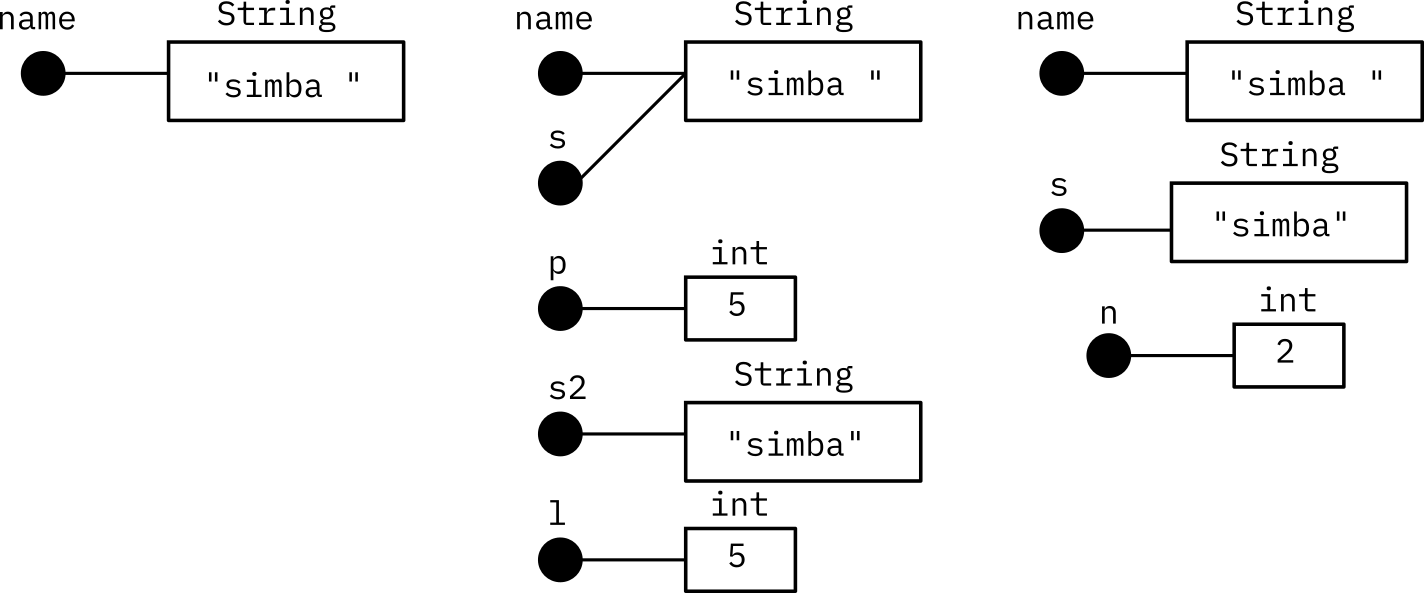
\includegraphics[ width=1.0\linewidth, height=\textheight, keepaspectratio]{./pics/png/snippet250.png}
    \label{fig:snippet250}
\end{figure}




\begin{lstlisting}
public int doThings(String s) {
  int p = 2;
  String s2 = s.trim();
  int l = s2.length(); // B
  return l / p;
}
/////
public void run() {
  String name = "simba "; // A
  int n = doThings(name); // C
}
\end{lstlisting}

\section{Riassunto del capitolo}

\begin{description}
    \item[Passaggio dei parametri] Il passaggio dei parametri avviene \emph{by value} o \emph{by reference} seguendo una semplice regola: il passaggio by value avviene sempre e solo per \emph{tipi primitivi}, mentre il passaggio by reference accade sempre e soltanto per \emph{tipi non primitivi}. Gli oggetti vengono perciò passati per riferimento, nel senso che avviene una copia del riferimento durante la chiamata ad una funzione. È possibile modificare e manipolare perciò gli oggetti all'interno delle funzioni tramite il riferimento copiato, con risultati visibili anche al termine dell'invocazione del metodo.
    \item[Il modificatore \texttt{final}] Il modificatore \texttt{final} è una keyword statica (ha effetti in atto di compilazione) che fa sì che il tipo primitivo o il riferimento ad un tipo non primitivo sia \emph{immutabile}. Dunque, tipi primitivi con modificatore \texttt{final} assumeranno l'aspetto di costanti, mentre riferimenti ad oggetti di tipi non primitivi con modificatore \texttt{final} non potranno fare riferimento ad altri oggetti. L'oggetto di tipo non primitivo che viene riferito da un riferimento con modificatore \texttt{final} può comunque cambiare il proprio stato. I casi d'uso sono, in ordine di importanza, la definizione di \emph{costanti}, il limitare la \emph{riusabilità} e il rimarcare l'\emph{immutabilità}. È buona norma applicare \texttt{final} a qualsivoglia variabile non debba essere modificata, sia negli argomenti di metodi che nei cicli for each.
    \item[Costanti object-wise] Field \emph{immutabili} che possono assumere valori differenti per ogni istanza di un oggetto, ma che una volta fissati non possono essere in nessun caso modificati. Solitamente, gli viene applicato un modificatore \texttt{final private}.
    \item[Costanti class-wise] Field \emph{globali immutabili} comuni a tutte le istanze. Essi vengono dichiarati come field e immediatamente il loro valore viene definito tramite la sintassi dell'assegnazione. Per essi si adopera la sintassi tutto maiuscolo, parole separate da underscore; ad esempio, \texttt{TITLE\_PREFIX}.
    \item[Scope] Proprietà \emph{statica} degli identificatori che esplicita in quale porzione di codice l'identificatore può essere adoperato -- essa è influenzata non solo dal tipo di oggetto, ma anche dai costrutti adoperati.
    \item[Lifetime] Proprietà \emph{dinamica} degli identificatori che esplicita l'intervallo di tempo entro il quale un oggetto o un riferimento esiste -- essa è influenzata dal tipo di oggetto.
    \item[Scope nei metodi] I riferimenti dichiarati nella signature di un metodo valgono in tutto e solo il metodo.
    \item[Scope nei costrutti] I riferimenti dichiarati nel codice sono visibili dal momento stesso della dichiarazione fino alla fine del blocco dove sono state dichiarate. Se dichiarate all'interno di cicli, esse sono visibili esclusivamente durante il singolo ciclo.
    \item[Il modificatore \texttt{protected}] Quarto modificatore d'accesso -- oltre a \texttt{private}, \texttt{public} e a quello di default -- che rende visibile l'entità soltanto \emph{nella classe che estende} direttamente o indirettamente la classe dove \texttt{protected} è utilizzato.
    \item[Scope per field, metodi e classi] Lo scope per field, metodi e classi è determinato dal modificatore d'accesso, secondo regole già viste sino ad ora.
    \item[Lifetime per tipi primitivi] Il tempo di vita per tipi primitivi è legato allo scope: essi esistono finché sono nello scope.
    \item[Lifetime per tipi non primitivi] I tipi non primitivi esistono a partire dallo statement che include il \texttt{new} per la loro creazione ed esistono \emph{almeno} finché sono referenziati. Per i tipi non primitivi \emph{non è noto} il momento esatto in cui essi cessano di esistere -- ovvero quando il \emph{garbage collector} si occupa di eliminarli dalla memoria.
\end{description}


\chapter{La memoria della Java Virtual Machine}

Contrariamente a quanto detto più volte, la memoria non è un blocco
destrutturato come il diagramma oggetti-riferimenti suggerirebbe in prima
analisi. La memoria della JVM è infatti organizzata in due zone distinte, lo
\textbf{stack} e lo \textbf{heap}:
\begin{itemize}
    \item lo \textbf{heap} è la zona della memoria dove risiedono i dati
        \emph{a lungo termine}. Lo heap è fatto per immagazzinare informazioni
        a lungo termine. Lo heap è \textbf{globale} \-- c'è un solo heap per
        ogni JVM. Nello heap sono collocati \textbf{tutti gli oggetti creati
        con \texttt{new}}, dunque \textbf{tutti gli oggetti non primitivi}, con i loro
        field. Gli \emph{array} stanno nello heap, anche quelli di tipi
        primitivi.
    \item lo \textbf{stack} è pensato per immagazzinare dati che vivono per
        meno tempo \-- \textbf{non è unico}, è organizzato in blocchi.
        Fisicamente, lo stack è costruito per disporre di un accesso più
        rapido. Nello stack ci vanno \textbf{tutti i riferimenti} e
        \textbf{tutti gli oggetti di tipo primitivo che non siano un field}, ad
        esempio tutte le variabili locali dichiarate all'interno dei metodi o
        nella loro signature. La dimensione di ogni blocco dello stack è
        determinabile al momento dell'invocazione del metodo \-- nel caso di
        vari percorsi possibili di computazione, viene scelta la massima
        quantità possibile. L'accesso allo stack è \emph{più veloce}.
\end{itemize}

Tipicamente, lo heap è molto più grande. Esso viene \emph{periodicamente
svuotato}. Lo stack è invece organizzato in blocchi \-- ogni qualvolta che
inizia l'esecuzione di un metodo viene \textbf{creato un nuovo blocco dello
stack} associato a tale metodo. Nel nuovo blocco sono introdotte tutte le
variabili locali dichiarate nel metodo. Il blocco viene prontamente rimosso
\textbf{al termine dell'esecuzione del metodo per cui è stato generato}

Nella memoria, \textbf{gli oggetti di tipo primitivo sono il loro riferimento}
\-- in altre parole, c'è un legame indissolubile fra il tipo primitivo ed il
loro riferimento, cioè non possono essere concettualmente separati. Per i tipi
primitivi, in definitiva, l'identificatore \emph{è} l'oggetto. Questo cambio di
mentalità spiega finalmente tutte le differenze e simitudini fra tipi primitivi
e non primitivi; in particolare: 
\begin{itemize}
    \item i tipi primitivi \textbf{hanno il medesimo lifetime dei riferimenti}
        \-- di fatto, sono la stessa cosa;
    \item i tipi primitivi non hanno un vero e proprio riferimento, dunque al
        passaggio vengono passati \textbf{by value}, diversamente dai tipi non
        primitivi che sono invece passati \textbf{by reference}; 
    \item l'assegnazione crea una \textbf{copia del valore} per i tipi primitivi,
        una copia del riferimento per gli oggetti di tipo non primitivo;
    \item l'operatore di uguaglianza \texttt{==} confronta il valore per i tipi
        primitivi, il riferimento per i tipi non primitivi;
    \item i tipi primitivi non possono fare riferimento a \texttt{null} \--
        essi non hanno veri e propri riferimenti!
\end{itemize}

Dunque, ciò che prima erano riferimenti a tipi primitivi, ora sono i tipi
primitivi stessi \-- nella stessa maniera, ciò che prima erano riferimenti a
tipi non primitivi, ora sono \textbf{indirizzi di memoria dello heap} dove gli
oggetti a cui fanno riferimento sono ospitati. Ad esempio \texttt{String*
0xAAF3} fa riferimento al tipo non primitivo \texttt{String} ospitato
all'indirizzo \texttt{0xAAF3}. Per i tipi primitivi si cambierà notazione, per
quelli non primitivi si manterrà la medesima.

La quantità di memoria occupata da un tipo primitivo è nota a priori:
\begin{itemize}
    \item \texttt{byte} richiede 1 byte;
    \item \texttt{short} richiede 2 byte;
    \item \texttt{int} richiede 4 byte;
    \item \texttt{long} richiede 8 byte;
    \item \texttt{float} occupa 4 byte;
    \item \texttt{double} occupa 8 byte;
    \item \texttt{char} occupa 2 byte;
    \item ed infine \texttt{boolean}, che richiede probabilmente 1 solo bit \--
        con la conseguenza che più variabili booleane sono solitamente inserite
        all'interno di un singolo byte.
\end{itemize}

I riferimenti, tipicamente, occupano 4 byte se la dimensione dello heap è
inferiore a 32GB, mentre occupano 8 byte per dimensioni dello heap maggiore.

\begin{figure}[h]
    \centering
    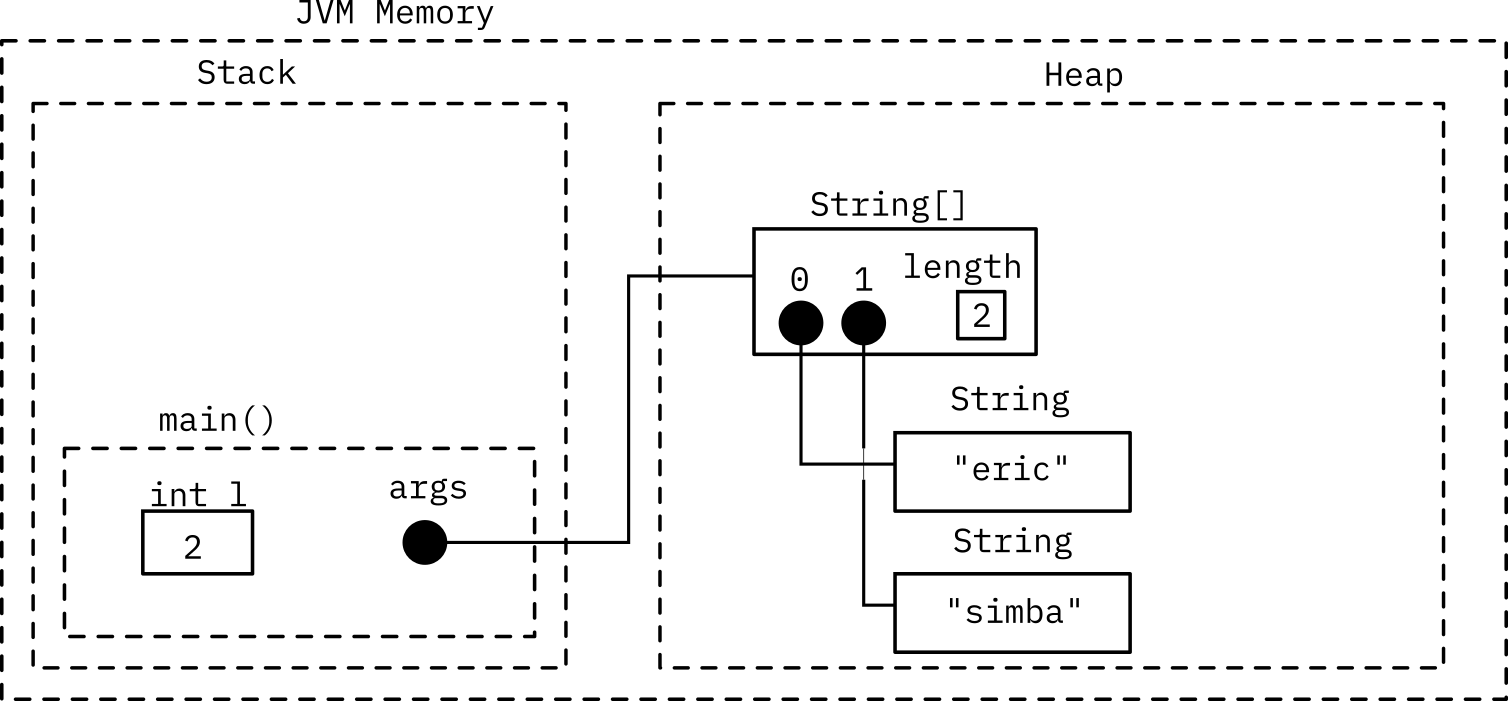
\includegraphics[ width=1.0\linewidth, height=\textheight, keepaspectratio]{./pics/png/snippet257.png}
    \caption{Diagramma oggetti-riferimenti aggiornato alle nuove nozioni di
    stack e heap.}
    \label{fig:snippet257}
\end{figure}



Per esempio,

\begin{lstlisting}
public static void main(String[] args) {
  int l = args.length;
}

eric@cpu:~$ java Greeter eric simba
\end{lstlisting}

con il diagramma a riferimenti ``aggiornato'' alla nuova notazione espresso in
Figura~\ref{fig:snippet257}. Si osservi come, all'inizio della memoria, gli
argomenti passati per linea di comando siano ospitati nello heap.

Sia il seguente frammento di codice

\begin{lstlisting}
public static void main(String[] args) {
  (new Main()).run();
}

public void run() {
  String name = "simba "; // A
  int n = doThings(name); // C
}

public int doThings(String s) {
  int p = 2;
  String s2 = s.trim();
  int l = s2.length(); // B
  return l / p;
}

/////
eric@cpu:~$ java Greeter
\end{lstlisting}

Nello stato A, lo stack è popolato esclusivamente dagli stack di
\texttt{main()}, dove nessun tipo primitivo è definito (vi è solo
\texttt{args}, di grandezza 4 byte) e di \texttt{run()}, anch'essa di
dimensione 8 byte, poiché ha al suo interno un riferimento di un tipo String ed
un e un \texttt{int} che ancora dovrà formarsi ma che si sa già che dovrà
esservi collocato. Nello heap vengono collocati \texttt{String[]} di
\texttt{args} e la stringa \texttt{"simba "}, approssimativamente occupando 4 e
12 byte. Nello stato B, viene creato un nuovo blocco dello stack per
\texttt{doThings()}. Vengono adoperati 16 byte, 8 per i due \texttt{int} ed
altri 8 per i due riferimenti. Il riferimento \texttt{s} farà riferimento alla
stringa nello heap. Al punto C vi è il ritorno del metodo \texttt{doThings()}:
il suo blocco nello stack viene rimosso, e viene finalmente allocato
l'\texttt{int} nello stack di \texttt{run()}.

\section{La garbage collection}

Nell'esempio di cui sopra, la stringa \texttt{"simba"}, dapprima con
riferimento \texttt{s2} e poi rimasta nello heap e senza alcun riferimento
associato è inutile; quando un oggetto non è più riferito, non è materialmente
utilizzabile, nessuna istruzione può coinvolgere l'oggetto \-- è perciò
\textbf{garbage}. La Java Virtual Machine dovrà dunque liberare la memoria in
qualche maniera, di modo da non rischiare di riempire l'intero spazio dello
heap. Si osservi che sono \emph{garbage} anche tutti gli oggetti che sono
riferiti soltanto da riferimenti anch'essi \emph{garbage}.

Rimuovere la garbage non è semplice. 
Non è infatti computazionalmente facile eliminare tutta la garbage, poiché ciò
equivarrebbe ad una ricerca nell'intero grafo per nodi non aventi archi
entranti \-- un compito che la JVM non può svolgere in continuazione.

L'operazione di rimuovere tutti i rettangoli senza un adeguato riferimento
dallo heap è detta \textbf{garbage collection}. La JVM decide ad intervalli
regolari \textbf{quando} e \textbf{cosa} considerare garbage, e la rimuove.
Di fondamentale importanza è il fatto che la garbage collection viene
effettuata solo in determinate circostanze \-- in quel caso, trova almeno un
po' di garbage, e la rimuove. Vi è un compromesso fra eliminare lo spazio
occupato dalla garbage ed eliminare un eccessivo overhead. Non esiste un unico
\textbf{garbage collector}: ci sono varie tecniche per realizzare un GC, con
diversi algoritmi che possono avere bassissimo overhead ma minore garbage
collection, o intensi burst di overhead con grandi raccolte di oggetti
inutilizzabili.

Tipicamente, l'impatto che il garbage collector ha sul sistema in esecuzione
dipende dal tipo di applicazione e dal momento in cui esso entra in azione.

Lo sviluppatore può \textbf{suggerire} alla JVM di eseguire la garbage
collection mediante il metodo \texttt{System.gc()}. La documentazione dice in
proposito

\begin{quote}
    \footnotesize{\texttt{static void gc()} Runs the garbage collector in the
        Java Virtual Machine.

Runs the garbage collector in the Java Virtual Machine.

Calling the \texttt{gc} method suggests that the Java Virtual Machine expend
effort toward recycling unused objects in order to make the memory they
currently occupy available for reuse by the Java Virtual Machine. When control
returns from the method call, the Java Virtual Machine has made a best effort
to reclaim space from all unused objects. There is no guarantee that this
effort will recycle any particular number of unused objects, reclaim any
particular amount of space, or complete at any particular time, if at all,
before the method returns or ever.
}
\end{quote}

La garbage collection ha un fondamentale aspetto positivo, quello di
\emph{togliere la responsabilità} allo sviluppatore del problema dello
svuotamento della memoria. Prima della garbage collection, lo sviluppatore
doveva esplicitamente liberare la memoria allocata con \texttt{malloc()}
mediante il termine \texttt{free()}. I problemi di questo approccio sono i
soliti \-- la possibilità di dimenticare i \texttt{free()} e conseguentemente
la memoria potrebbe terminare lo spazio libero, oppure l'esecuzione di
\texttt{free()} su indirizzi errati, la possibilità di scrivere su una memoria
in precedenza allocata. Con la garbage collection, al prezzo di piccoli momenti
in cui la garbage collection interviene e blocca l'applicazione in esecuzione,
questi problemi legati allo sviluppo non esistono più.

La GC richiede molto tempo, non è predicibile \emph{quanto} e non è
predicibile nemmeno \emph{quando}; potrebbe addirittura essere indesiderato in
talune applicazioni o momenti particolari. Il grafo realizzato dagli oggetti e
dai loro riferimenti potrebbe essere \emph{aciclico} e molto grande. È
possibile migliorare le performance del GC, modificandone le impostazioni
oppure chiamandolo direttamente all'interno del codice.

\section{Impostare la dimensione della memoria della JVM}

La dimensione della memoria della JVM può essere impostata tramite flag da riga
di comando, in particolare con il flag \texttt{-X}:
\begin{itemize}
    \item \texttt{-Xms} indica la dimensione di partenza dello heap \-- la
        dimensione dello heap può cambiare poiché si tratta di una macchina
        virtuale;
    \item \texttt{-Xmx} indica la dimensione massima dello heap;
    \item \texttt{-Xss} determina la dimensione dello stack \-- solo uno poiché
        ha una \emph{dimensione fissa}.
\end{itemize}

Ad esempio, l'invocazione seguente

\begin{verbatim}
eric@cpu:~$ java MyBigApplication -Xmx8G
\end{verbatim}

imposta una massima dimensione dello heap pari a 8 Gigabyte.

Tipici errori durante l'esecuzione relativi alla mancanza di memoria sono i due
seguenti,
\begin{itemize}
    \item \texttt{java.lang.OutOfMemoryError: Java heap space} quando lo heap è
        eccessivamente riempito, o non vi sono ``buchi'' dove inserire i nuovi
        oggetti o array;
    \item \texttt{java.lang.StackOverFlowError} quando avviene uno stack
        overflow, nel caso in cui lo stack sia stato impostato a dimensione
        troppo piccola e vengano allocate troppe variabili in esso.
        Difficilmente lo stack è riempibile: in esso vi sono contenute
        variabili molto piccole. Tipicamente, anche la ricorsione senza
        condizione d'arresto può provocare lo stack overflow.
\end{itemize}


\section{Le wrapper classes}

Esistono delle classi, dette \textbf{wrapper classes}, che hanno la funzione di
contenere i valori dei tipi primitivi pur non essendo tipi primitivi \-- tali
classi permettono di modellare i tipi primitivi come non primitivi, avendo
anche la potenzialità di svolgere metodi su di essi.

Le classi sono
\begin{itemize}
    \item \texttt{Integer} per gli \texttt{int};
    \item \texttt{Double} per i \texttt{double};
    \item \texttt{Character} per i \texttt{char};
    \item \texttt{Boolean} per i \texttt{boolean};
    \item e così via.
\end{itemize}

Le wrapper classes sono oggetti \textbf{immutabili}, come le stringhe, e si
collocheranno nella memoria heap.

La classe integer, secondo la documentazione,
\begin{quote}
    \footnotesize{The \texttt{Integer} class wraps a value of the primitive type \texttt{int} in an object. An object of type \texttt{Integer} contains a single field whose type is int.

In addition, this class provides several methods for converting an \texttt{int} to a String and a String to an \texttt{int}, as well as other constants and methods useful when dealing with an int.
}
\end{quote}

La classe \texttt{Integer} contiene anche delle costanti:
\begin{itemize}
    \item \texttt{static int BYTES} che contiene il numero di bytes usato per
        rappresentare un \texttt{int} in complemento a due;
    \item \texttt{MAX\_VALUE};
    \item \texttt{MIN\_VALUE};
\end{itemize}

e contengono gli pseudo-costruttori 

\begin{quote}
    \footnotesize{\texttt{static int parseInt(String s)} Parses the string argument as a signed decimal integer.

        \texttt{static int parseInt(String s, int radix)} Parses the string argument as a signed integer in the radix specified by the second argument.

    \texttt{static Integer valueOf(int i)} Returns an Integer instance representing the specified int value}
\end{quote}

per esempio

\begin{lstlisting}
int n = Integer.parseInt("1100110", 2); // -> 102
\end{lstlisting}

ed altri esempi, relativi al return

\begin{quote}
    \footnotesize{\texttt{int intValue()} Returns the value of this Integer as an int.

        \texttt{long longValue()} Returns the value of this Integer as a long
after a widening primitive conversion.}
\end{quote}

\subsection{Autoboxing ed autounboxing}

In Java esistono anche gli \textbf{autoboxing} e gli \textbf{autounboxing} \--
speciali scorciatoie sintattiche adottate per semplificare l'uso delle wrapper
classes. Ad esempio,

\begin{lstlisting}
public void doIntThings(int n) { /* ... */ }
public void doIntegerThings(Integer n) { /* ... */ }

Integer i = 3; // autoboxing
doIntThings(i); // autounboxing

int n = 3; // autoboxing
doIntegerThings(n); //autounboxing

Integer i = 2; // autoboxing
i++; // autounboxing, esecuzione del '++', autoboxing
\end{lstlisting}

che viene tradotto in

\begin{lstlisting}
Integer i = Integer.valueOf(3);
doIntThings(i.intValue());

int n = 3;
doIntegerThings(Integer.valueOf(n));

Integer i = Integer.valueOf(2);
i = Integer.valueOf(i.intValue()+1);
\end{lstlisting}

In generale è bene adoperare la classe \texttt{int} qualora non fosse
assolutamente richiesta una wrapper class.

A livello di memoria, gli \texttt{Integer} sono disposti nello heap e hanno un
riferimento nello stack, mentre gli \texttt{int} sono direttamente disposti
nello stack. Gli \texttt{Integer} tipicamente producono maggiore lavoro per il
garbage collector, in quanto sono immutabili e tendono ad accumularsi ad ogni
modifica.

Attenzione però: per le classi wrapper \textbf{non c'è unboxing per
l'operazione di uguaglianza} \texttt{==}! L'autounboxing avviene \textbf{solo}
se uno dei due operandi è un tipo primitivo; invece \textbf{non avviene} nel
caso in cui \textbf{entrambi gli operandi sono wrapper classes}, o comunque
quando entrambi sono oggetti.

Ad esempio,

\begin{lstlisting}
Integer n = 300;
Integer m = 300;
int k = 300;
System.out.printf("n ?= m -> %b%n", n==m); // -> false!!!
System.out.printf("n ?= k -> %b%n", n==k); // -> true!!!
\end{lstlisting}

Nel caso in cui \texttt{(n+1)==(m+1)} produce \texttt{true} poiché avviene
l'autounboxing dei numeri di sopra, e vengono paragonati i valori \texttt{301
== 301}, che forniscono il risultato \texttt{true}.

È meglio adoperare il metodo \texttt{equals()} quando vi è da fare un paragone
(l'IDE lo evidenzia).

\section{Riassunto del capitolo}

\begin{description}
    \item[Heap] Zona di memoria dove risiedono tutti gli \emph{oggetti di tipo non primitivo}, da considerarsi a lungo termine. In esso sono collocati tutti gli oggetti creati con la parola chiave \textbf{new}, dunque tutti gli oggetti non primitivi risiedono nello heap. Gli array stanno nello heap---anche quelli composti da tipi primitivi. Poiché nello heap risiedono gli oggetti di tipo non primitivo con tutti i loro dati, anche i field---siano essi di tipo primitivo o non primitivo---risiedono nello heap. La dimensione dello heap è determinata \emph{dinamicamente}. Esiste un solo heap per ogni istanza di Java Virtual Machine. Lo heap è generalmente molto più grande dello stack.
    \item[Stack] Zona di memoria dove risiedono tutti gli \emph{oggetti di tipo primitivo} che non siano field e tutti i \emph{riferimenti}. Esso è detto `stack' in quanto per ogni execution thread ciascuna chiamata ad un metodo produce un nuovo blocco, che viene poi liberato appena il metodo consegna il valore di ritorno. Dunque, tutte le variabili locali dichiarate all'interno di metodi o signature. La dimensione di ogni blocco dello stack è predeterminabile dal momento dell'invocazione del metodo, scegliendo sempre la massima quantità di memoria necessaria al percorso più critico dal punto di vista dell'allocazione in memoria; oltre a ciò, l'accesso allo stack è generalmente più veloce dell'accesso allo heap.
    \item[Passaggio dei parametri in Java] In Java, esistono due tipi di passaggio di parametri: \emph{by value} e \emph{by reference}. Il primo è prerogativa dei riferimenti e dei tipi primitivi, il secondo invece è specifico degli oggetti. Per i tipi primitivi, gli oggetti di tipo primitivo sono il loro stesso riferimento: i due concetti coincidono, ed essi non possono essere riferiti da altri riferimenti. Per i tipi primitivi, l'identificatore è l'oggetto stesso; l'assegnazione creerà una \emph{copia} del loro valore. Diversamente, per i tipi non primitivi il riferimento è un concetto distinto dall'oggetto, dunque più riferimenti possono riferire al medesimo oggetto. I tipi primitivi non possono pertanto fare riferimento a \texttt{null} (invece i tipi non primitivi possono) ed infine l'operatore di uguaglianza per i tipi non primitivi ne verifica l'uguaglianza del riferimento, non dell'oggetto.
    \item[Memoria richiesta per allocare tipi primitivi] La memoria richiesta per allocare tipi primitivi è nota a priori: 1 byte per \texttt{byte}, 2 byte per \texttt{short} e \texttt{char}, 4 byte per \texttt{int} e \texttt{float} ed infine 8 byte per \texttt{long} e \texttt{double}. I \texttt{boolean} occupano al minimo 1 bit ed almeno 8 bit: possono essere collassati fino a 8 \texttt{boolean} in un unico byte. 
    \item[Memoria richiesta per allocare riferimenti] I riferimenti occupano 4 byte per dimensioni dello heap inferiori a 32GB, 8 byte per dimensioni dello heap superiori a 32GB.
    \item[Garbage collection] Procedura secondo la quale lo heap viene svuotato degli oggetti senza un adeguato riferimento, cioè oggetti i quali riferimenti sono tutti fuori dallo scope del programma in esecuzione, al fine di prevenire il riempimento della memoria e l'eccessivo consumo di essa. La garbage collection è, in generale, una tecnica che comprende famiglie di algoritmi di diverse prestazioni ed efficacia per determinare gli oggetti nello heap da eliminare, con tipicamente un compromesso fra tempo impiegato per la collection ed efficacia. Il garbage collector può essere invocato dalla Java Virtual Machine in qualsiasi momento, non predeterminabile---è comunque possibile suggerire esplicitamente nel codice tramite il metodo statico \texttt{System.gc()} di eseguire la garbage collection, senza tuttavia garanzia di risultati. In generale, la garbage collection è un ottimo sistema per ridurre l'onere della gestione della memoria allo sviluppatore, benché introduca una perdita di performance non predicibile, non determinabile a priori.
    \item[Parametri a riga di comando per specificare la memoria disponibile per la JVM] Vari parametri a riga di comando esistono (su ambiente Linux, digitare \texttt{man java}): \texttt{-Xms} indica la dimensione di partenza dello heap; \texttt{-Xmx} indica la dimensione massima dello heap; \texttt{-Xss} permette di specificare la dimensione massima dello stack. Errori associati alla memoria sono \texttt{java.lang.OutOfMemoryError} e \texttt{java.lang.StackOverFlowError}.
    \item[Wrapper classes] Classi wrapper per tipi primitivi, una per ciascun tipo primitivo. Sono dotate di field statici quali \texttt{BYTES}, \texttt{MAX\_VALUE} e \texttt{MIN\_VALUE} e di pseudo-costruttori per fare il parsing del tipo da una stringa e per restituire il valore (specifici getter e setter).
    \item[Autoboxing e autounboxing] Scorciatoie sintattiche del linguaggio Java che consentono di trattare nel codice i tipi wrapper come tipi primitivi, eseguendo automaticamente la conversione da tipi primitivi a tipi non primitivi. L'autoboxing e l'autounboxing avviene esclusivamente se un tipo wrapper non primitivo deve entrare in contatto in un'espressione con un tipo primitivo compatibile.
\end{description}




\chapter{Input ed output avanzati}

Le due maniere fondamentali per ottenere l'input sono mostrate di seguito, ed
erano già state illustrate tempo fa,

\begin{lstlisting}
BufferedReader reader = new BufferedReader(
  new InputStreamReader(System.in)
);
/* ... */
String line = reader.readLine();

Scanner scanner = new Scanner(System.in);
/* ... */
String s = scanner.next();
int n = scanner.nextInt();
double d = scanner.nextDouble();
\end{lstlisting}

Un'importante astrazione da introdurre è quella dello \textbf{stream}. Uno
stream è un flusso di dati, un ``tubo'' con sequenzialità \emph{fra due
endpoint}, con una \emph{direzione}, ed un \emph{tipo di dati}.

Due modelli fondamentali sono i seguenti,

\begin{itemize}
    \item l'\textbf{output stream} ad un dispositivo dove i dati possono essere
        scritti come \texttt{byte[]};
    \item l'\textbf{input stream} da un dispositivo da cui i dati possono
        essere letti come \texttt{byte[]};
\end{itemize}

TODO disegni 277

La rappresentazione adoperata sarà quella in Figura~\ref{fig:stream277}: essa
rappresenta il \emph{generico dispositivo}, e si tratta di un'astrazione del
dispositivo. L'interazione con uno stream avviene dapprima creando lo stream, e
poi reiterando la lettura o la scrittura di \texttt{byte[]} array sullo stream.
Un \textbf{device} potrebbe essere qualunque cosa \-- un file, la memoria, la
rete. 

Un output stream può avere delle \emph{capacità di processamento} dei dati. Si
potrebbe voler comprimere o decomprimere il flusso di \texttt{byte[]}, o la
trasformazione di \texttt{byte[]} da (o in) altri tipi. Impilare gli stream di
fila è una maniera per realizzare un'operazione dopo l'altra.

Le classi che realizzano gli stream sono \texttt{Input\-Stream} ed
\texttt{Output\-Stream}. Uno stream si può comporre sovrapponendolo ad un altro
stream: il risultato è comunque uno stream nella medesima direzione. Ciascuno
stream è un \textbf{device} per il dispositivo sopra. Ciascuno stream, dunque,
offre la medesima interfaccia; questo particolare design si chiama
\textbf{filter pattern} \-- l'idea è di fornire un'``unica'' interfaccia alle
applicazioni che hanno bisogno di fare input\----output, al contempo
realizzando alcune funzionalità. Ciascun livello della pila di stream fornisce
un ``filtraggio'' delle funzionalità. 

Non c'è bisogno di modificare il codice: grazie al \textbf{polimorfismo}, il
tipo del device farà sì che lo stream si comporti in maniera ogni volta
differente. Lo stesso vale per i differenti processing. È possibile anche
comporre tipi di dati maggiormente complessi, ciò che si fa è porre in cima
alla pila un \texttt{Input\-Stream} che è in grado di gestire un flusso
\texttt{int[]}.

Vi sono molti tipi di \texttt{Input\-Stream}, ne vedremo soltanto alcuni.

\section{I/0 di byte}

La classe \texttt{Output\-Stream},

\begin{quote}
    \footnotesize{This abstract class is the superclass of all classes
    representing an output stream of bytes. An output stream accepts output
bytes and sends them to some sink.}
\end{quote}

ed ha i metodi,
\begin{quote}
    \footnotesize{\texttt{void 	close()} 	Closes this output stream and releases any system resources associated with this stream.

            \texttt{void 	flush()} 	Flushes this output stream and forces any buffered output bytes to be written out.

    \texttt{static OutputStream 	nullOutputStream()} 	Returns a new OutputStream which discards all bytes.

    \texttt{void 	write(byte[] b)} 	Writes b.length bytes from the specified byte array to this output stream.

    \texttt{void 	write(byte[] b, int off, int len)} 	Writes len bytes from the specified byte array starting at offset off to this output stream.

\texttt{abstract void 	write(int b)} 	Writes the specified byte to this output stream.}

\end{quote}

e scrive soltanto \texttt{byte[]}.

La classe è \textbf{abstract}, cioè non può essere utilizzata o istanziata.

L'errore \texttt{OutputStream.nullOutputStream()} fornisce un device che
rifiuta sempre tutti i byte.

Più in dettaglio,
\begin{quote}
    \footnotesize{\texttt{void 	write(byte[] b, int off, int len)} 	Writes len bytes from the specified byte array starting at offset off to this output stream.

Writes len bytes from the specified byte array starting at offset off to this output stream. The general contract for write(b, off, len) is that some of the bytes in the array b are written to the output stream in order; element b[off] is the first byte written and b[off+len-1] is the last byte written by this operation.}
\end{quote}

Un uso pratico può essere il seguente,

\begin{lstlisting}
byte[] data = /* ... */
OutputStream os = /* ... */
os.write(data, 0, 3); //A
os.write(data, 3, 2); //B
os.write(new byte[2]); //C
\end{lstlisting}

Lo stream:
\begin{itemize}
    \item dopo l'esecuzione di A, contiene 3 byte \-- il cursore punta 3;
    \item dopo l'esecuzione di B, contiene 5 byte \-- il cursore punta 5;
    \item dopo l'esecuzione di C, contiene infine 7 byte \-- il cursore punterà
        sull'ottavo byte, indice 7.
\end{itemize}

Vediamo ora con maggiore dettaglio i metodi \texttt{write()},

\begin{lstlisting}
write(byte[] b, int off, int len)
\end{lstlisting}

\begin{quote}
    \footnotesize{The general contract for \texttt{write(b, off, len)} is that some of
        the bytes in the array \texttt{b} are written to the output stream in order; element
        \texttt{b[off]} is the first byte written and \texttt{b[off+len-1]} is the last byte written by
this operation.}
\end{quote}

\begin{lstlisting}
write(byte[] b)
\end{lstlisting}

\begin{quote}
    \footnotesize{The general contract for \texttt{write(b)} is that it should have
        exactly the same effect as the call \texttt{write(b, 0, b.length)}.
}
\end{quote}

In altre parole, la documentazione ci fornisce il contratto che dovremmo
seguire nel caso facessimo l'override del metodo \texttt{write()} \-- le
sottoclassi di \texttt{Output\-Stream} \textbf{devono} almeno fornire un metodo
che è in grado di scrivere un singolo byte. Il seguente metodo andrebbe riscritto ugualmente,

\begin{lstlisting}
write(byte[] b, int off, int len)
\end{lstlisting}

poiché chiama, uno dopo l'altro, \texttt{write(b[i])}, cioè fa una cosa simile

\begin{lstlisting}
public void write(byte[] b, int off, int len) {
  for (int i = off; i < off+len; i++) {
    write(b[i]); // calls write
  }
}
\end{lstlisting}

ed è poco efficiente. Un esempio di scarsa efficienza è l'uso di esso per un protocollo di rete;
a livello di TCP è meglio inviare un numero maggiore di byte per volta. C'è
infatti un costo fisso (overhead) nella scrittura su dispositivo, a prescindere
dalle dimensioni dei dati, nella scrittura di un maggior numero di byte per
volta. Anche i vecchi Hard Disk possono godere di un beneficio
nell'ottimizzazione del metodo \texttt{write(byte[] b, int off, int len)}.

\subsection{Associazione con i device}

In pieno stile UNIX, Java tratta tutti i device con la medesima interfaccia.
Dunque, si desideri accedere ad un \emph{file}, ad una \emph{memoria} o ad un
\emph{dispositivo di rete}, il codice da scrivere è del tutto simile nei tre
casi:

\begin{itemize}
    \item nel caso del \emph{file}:
\begin{lstlisting}
OutputStream os = new FileOutputStream(/* ... */);
byte[] data = /* ... */
os.write(data);
\end{lstlisting}
    \item nel caso di un \emph{dispositivo di rete}:
\begin{lstlisting}
Socket socket = /* ... */
OutputStream os = socket.getOutputStream();
byte[] data = /* ... */
os.write(data);
\end{lstlisting}
    \item nel caso di una \emph{memoria}:
\begin{lstlisting}
OutputStream os = new ByteArrayOutputStream();
byte[] data = /* ... */
os.write(data);
\end{lstlisting}
\end{itemize}

A seconda del dispositivo però varierà il modo in cui la JVM dovrà
interfacciarsi con esso. Per esempio, nel caso di \texttt{socket},
il sistema operativo sottostante dovrà creare un corrispondente socket
con relativa connessione TCP \-- prima di poterla adoperare, dunque, essa dovrà
essere creata.

La classe \texttt{File} modella l'ubicazione di un file, con le corrispondenti
\emph{system calls} dentro e sotto la JVM.

Dalla documentazione della classe \texttt{FileOutputStream},
\begin{quote}
    \footnotesize{A file output stream is an output stream for writing data to
    a File or to a FileDescriptor. \textbf{Whether or not a file is available or may be
    created depends upon the underlying platform}. Some platforms, in particular,
allow a file to be opened for writing by only one FileOutputStream (or other
file-writing object) at a time. In such situations the constructors in this
class will fail if the file involved is already open.

\texttt{FileOutputStream(File file)} 	Creates a file output stream to write to the file represented by the specified File object.

\texttt{FileOutputStream(File file, boolean append)} 	Creates a file output stream to write to the file represented by the specified File object.

\texttt{FileOutputStream(String name)} 	Creates a file output stream to write to the file with the specified name.

\texttt{FileOutputStream(String name, boolean append)} 	Creates a file output stream to write to the file with the specified name.
}
\end{quote}

Si noti innanzitutto che la classe \texttt{FileOutputStream} gestisce l'output
stream per la scrittura verso oggetti di classe \texttt{File} e
\texttt{FileDescriptor}; l'effettiva riuscita della scrittura \textbf{dipende
dal sistema operativo sottostante}. Per alcune di esse, ad esempio, potrebbe
essere possibile utilizzare esclusivamente un singolo \texttt{FileOutputStream}
per volta.

Nella seconda parte, sono riportati alcuni costruttori degni di nota \-- si
noti il booleano \texttt{append}, di default \texttt{false}, il quale ci
fornisce la possibilità di ``appendere'' i dati al file (anziché ricominciare
con la scrittura dall'inizio del file).

Per quanto riguarda la classe \texttt{socket} osserviamo un metodo in
particolare,
\begin{quote}
    \footnotesize{\texttt{OutputStream 	getOutputStream()}	Returns an output
    stream for this socket.}
\end{quote}
dove l'utente non è tenuto a sapere necessariamente la classe dell'output
stream fornito da \texttt{getOutputStream()}.

Esiste poi la classe \texttt{ByteArrayOutputStream}: essa modella il concetto

\begin{quote}
    \footnotesize{This class implements an output stream in which the data is
    written into a byte array. The buffer automatically grows as data is
written to it. The data can be retrieved using \texttt{toByteArray()} and \texttt{toString()}.}

\texttt{int 	size()} 	Returns the current size of the buffer.
\texttt{byte[] 	toByteArray()} 	Creates a newly allocated byte array.
\end{quote}

in pratica, modella un \textbf{buffer} (buffer è il nome gergale per un byte
array).

L'utilizzo del \texttt{ByteArrayOutputStream} è nella maniera seguente,

\begin{lstlisting}
ByteArrayOutputStream baos = new ByteArrayOutputStream();
byte[] data = /* ... */
baos.write(data);
byte[] written = baos.toByteArray();
System.out.println(Arrays.equals(data, written)); // -> true
\end{lstlisting}

con una prima invocazione del metodo \texttt{write()} contentente i dati da
scrivere, e successivamente da estrarre con metodo \texttt{toByteArray()}.

Tutte le classi ``output stream'' viste fino ad ora sono sottoclassi
(ereditano) della classe \texttt{Output\-Stream}.

\subsection{L'End Of Stream}

L'\textbf{end of stream} (EOS) è un marcatore logico di cui non interessa la
dimensione, il cui scopo è delimitare lo stream \-- oltre a tale marcatore, non
c'è più nulla. Il marcatore EOS è inserito dal comando \texttt{os.close()}, il
che chiude definitivamente lo stream, e non è più possibile scrivere nulla con
esso:

\begin{lstlisting}
byte[] data = /* ... */
OutputStream os = /* ... */
os.write(data, 0, 3); //A
os.close(); //B
\end{lstlisting}

Al punto A è ancora possibile scrivere dati, la ``freccia'' punterà al prossimo
byte da scrivere. Al punto B invece viene collocato l'End of Stream alla fine
della sequenza, e nessun altro dato sarà scrivibile \-- lo stream è
definitivamente chiuso.

Rispettare la chiusura degli output stream è di fondamentale importanza a
livello del sistema operativo, dove un output stream potrebbe inificiare le
prestazioni dell'intero sistema, o nei casi migliori, consumare semplicemente
inutili risorse.

Dalla documentazione della classe \texttt{OutputStream.close()}:
\begin{quote}
    \footnotesize{

    Closes this output stream and releases any system resources associated with
    this stream. The general contract of close is that it closes the output
    stream. A closed stream cannot perform output operations and cannot be
    reopened.

    The \texttt{close} method of OutputStream does nothing.
}
\end{quote}

In altre parole, la classe \texttt{Output\-Stream} non modella alcun device in
particolare, \textbf{esso modella una generica risorsa di sistema}.

Un altro caso particolare è quello della classe \texttt{ByteArrayOutputStream},
per cui la chiusura non ha alcun effetto \-- i metodi comuni possono essere
chiamati anche successivamente alla chiusura del byte array output stream.

\section{L'input stream}

La classe \texttt{Input\-Stream} è la \emph{superclasse di tutte le classi che
rappresentano un input stream di byte}.


\begin{quote}
    \footnotesize{\texttt{abstract int 	read()} 	Reads the next byte of data from the input stream.
        \texttt{int 	read(byte[] b)} 	Reads some number of bytes from the input stream and stores them into the buffer array b.
    \texttt{int 	read(byte[] b, int off, int len)} 	Reads up to len bytes of data from the input stream into an array of bytes.}
\end{quote}

L'input stream legge solo array \texttt{byte[]}, e il metodo
\texttt{InputStream.nullInputStream()} fornisce un dispositivo di input dal
quale non vi sono byte da leggere (EOS collocato alla posizione 0,
l'equivalente di \texttt{/dev/null}).

In lettura, si adopera il metodo \texttt{read()}. In particolare,
\begin{quote}
    \footnotesize{\texttt{int 	read(byte[] b, int off, int len)} 	Reads up to
    len bytes of data from the input stream into an array of bytes.

Reads up to len bytes of data from the input stream into an array of bytes. An
\texttt{attempt} is made to read as many as len bytes, but a smaller number may be read.
The number of bytes actually read is returned as an integer.}
\end{quote}

Il numero di byte letti viene restituito sotto forma di intero.

Inoltre, un po' come nel caso della scrittura \texttt{read(b)} è \emph{per
contratto} come eseguire \texttt{read(b, 0, b.length)}.

\begin{lstlisting}
byte[] buffer = new byte[100];
InputStream is = /* ... */ //A - cursor at 0
is.read(buffer, 0, 4); //B - cursor at 4
is.read(buffer, 4, 1); //C - cursor at 5
\end{lstlisting}

In pari modo, l'associazione con il device è simile a quella con il metodo
\texttt{write}:

\begin{lstlisting}
//File:
InputStream is = new FileInputStream(/* ... */);
byte[] buffer = new byte[100];
is.read(buffer, 0, 10);

//Network (TCP):
Socket socket = /* ... */
InputStream is = socket.getInputStream();
byte[] buffer = new byte[100];
is.read(buffer, 0, 10);

//Memory:
InputStream is = new ByteArrayInputStream(/* ... */);
byte[] buffer = new byte[100];
is.read(buffer, 0, 10);
\end{lstlisting}

Le similitudini non fiscono qua: si possono infatti istanziare le sottoclassi
figlie di (che ereditano da) \texttt{Input\-Stream}, infatti secondo la
documentazione della classe \texttt{FileInputStream}

\begin{quote}
A FileInputStream obtains input bytes from a file in a file system. What files are available depends on the host environment.

\texttt{FileInputStream(File file)} 	Creates a FileInputStream by opening a connection to an actual file, the file named by the File object file in the file system.
\texttt{FileInputStream(String name)} 	Creates a FileInputStream by opening a connection to an actual file, the file named by the path name name in the file system.
\end{quote}

Un oggetto della classe \texttt{ByteArrayInputStream} {\footnotesize contains an
internal buffer} (il dispositivo) {\footnotesize that contains bytes that may be
read from the stream. An internal counter keeps track of the next byte to be
supplied by the read method.}

Essa ha come costruttori 

\begin{quote}
    \footnotesize{\texttt{ByteArrayInputStream(byte[] buf)} 	Creates a
    ByteArrayInputStream so that it uses buf as its buffer array.}
\end{quote}

\subsection{Differenze nell'astrazione fra input ed output stream}

La principale differenza fra input ed output stream risiede nella gestione
dell'End of Stream. Se infatti per un output stream \textbf{non vi sono in
principio limiti nella scrittura} e bisognerà piazzare un EOS qualora servisse
chiudere il dispositivo, per un input stream \textbf{i dati leggibili sono
limitati}, poiché potrebbe esistere già un EOS nel device che
\texttt{Input\-Stream} astrae.

Sia infatti nel caso in cui si faccia uso di un \texttt{FileInputStream} che di
un \texttt{ByteArrayInputStream}, i device avranno una dimensione limitata,
perciò esisterà un EOS ad essi relativo (o comunque il device avrà una
dimensione limitata di dati da leggere, almeno temporaneamente).

Infatti, esiste una distinzione netta nel caso di lettura con EOS e senza:
\begin{quote}
    \footnotesize{\texttt{int 	read(byte[] b, int off, int len)} 	Reads up to
        len bytes of data from the input stream into an array of bytes.

Reads up to len bytes of data from the input stream into an array of bytes.
\textbf{An attempt is made to read as many as len bytes, but a smaller number
may be read}. The number of bytes actually read is returned as an integer.

This method \textbf{blocks until input data is available, end of file is
detected, or an exception is thrown}.

If len is zero, then no bytes are read and 0 is returned; otherwise, there is
an attempt to read at least one byte. If no byte is available because the
stream is at end of file, the value -1 is returned; otherwise, at least one
byte is read and stored into b.}
\end{quote}

In altre parole, al termine della disponibilità dei dati proveniente da un
input buffer, o viene trovato un EOS, oppure il metodo viene bloccato finché
non sono disponibili altri dati.

Nel caso il prossimo byte sia un EOS, viene restituito immediatamente -1, nel
caso di nessun dato disponibile metti in attesa. Diversamente, se vi sono dati
disponibili, li leggerà tutti fino ad un massimo di \texttt{len} bytes letti
restituendo il numero di byte letti.

Per esempio, si supponga un device contenente 5 byte all'istante zero, e
ricevente al secondo 10 altri 3 byte, seguiti da un EOS. Eseguendo le
istruzioni di seguito si otterrebbe l'effetto indicato nei commenti,

\begin{lstlisting}
is.read(buf, 0, 3);
// t=0 -> t~0, ret 3
is.read(buf, 0, 3);
// t~0 -> t~0, ret 2
is.read(buf, 0, 3); // BLOCK!
// t~0 -> t~10, ret 3
is.read(buf, 0, 3);
// t~10 -> t~10, ret -1
\end{lstlisting}

dunque incontrando un EOS durante la lettura si otterrebbe il valore di ritorno
-1.

Il blocco e l'attesa di input del metodo \texttt{read()} sono necessari per
l'attesa di input: si pensi all'\texttt{Input\-Stream} \texttt{System.in}, in
questo caso finché non viene premuto il tasto di ``invio'' l'input stream non
può ricevere alcunché. Fra l'altro, il \texttt{close()} su \texttt{System.in}
non ha alcun effetto. Parimenti, per un dispositivo di rete \texttt{InputStream
getInputStream()} legge dati dal socket mentre essi arrivano, e mette il tutto
in attesa finché non arrivano altri dati.

\subsection{Lettura e scrittura di un file}

La classe \texttt{File} eredita direttamente da \texttt{Object} e,
contrariamente a quanto ci si possa aspettare, \textbf{non rappresenta un
file}: {\footnotesize An abstract representation of file and directory pathnames.
User interfaces and operating systems use system-dependent pathname strings to
name files and directories. This class presents an abstract, system-independent
view of hierarchical pathnames.}

La classe \texttt{File} non appartiene alla gerarchia degli stream \-- si
limita infatti a modellare i \textbf{nomi di percorso di file e directory}. I
file sono dunque modellati nel senso di nomi di percorso, anch'essi aventi una
struttura ad albero. I \texttt{File} descrivono in termini formali come
descrivere un pathname, con l'ultimo elemento della gerarchia file o directory.
I file sono dunque i nodi terminali \-- ogni directory ha 0 o più nodi figlio.

Tramite la classe \texttt{File} è possibile rinominare i file ed eseguire altre
operazioni analoghe,

\begin{quote}
    \footnotesize{\texttt{boolean 	canExecute()} 	Tests whether the application can execute the file denoted by this abstract pathname.

\texttt{boolean 	canRead(}) 	Tests whether the application can read the file denoted by this abstract pathname.

\texttt{boolean 	canWrite(}) 	Tests whether the application can modify the file denoted by this abstract pathname.

\texttt{boolean 	delete(}) 	Deletes the file or directory denoted by this abstract pathname.

\texttt{boolean 	exists(}) 	Tests whether the file or directory denoted by this abstract pathname exists.

\texttt{boolean 	isDirectory(}) 	Tests whether the file denoted by this abstract pathname is a directory.

\texttt{String[] 	list(}) 	Returns an array of strings naming the files and directories in the directory denoted by this abstract pathname.

\texttt{File[] 	listFiles(}) 	Returns an array of abstract pathnames denoting the files in the directory denoted by this abstract pathname.

\texttt{boolean 	mkdir(}) 	Creates the directory named by this abstract pathname.

\texttt{boolean 	renameTo(File dest}) 	Renames the file denoted by this abstract pathname.

\texttt{boolean 	setExecutable(boolean executable}) 	A convenience method to set the owner's execute permission for this abstract pathname.}
\end{quote}

non è tuttavia possibile leggere o scrivere dai file (non sono stream!). 

L'apertura avviene tramite lo stream \texttt{FileOutputStream(File file)} o
\texttt{FileOutputStream(String name)}. Quando si esegue un tentativo di
scrittura di un file tramite uno stream, questi accederà al file ``reale''
ospitato tramite il sistema operativo mediante l'oggetto di classe
\texttt{File}. Qualora la stringa dello stream non rappresenti un file
realmente esistente in memoria, \textbf{questi viene creato}. Attenzione,
poiché \textbf{il contenuto del file viene cancellato se non viene specificato
il flag booleano \texttt{append}}.

L'effettiva scrittura e lettura di un file dipendono dal sistema operativo
sottostante.

\subsection{Copia ed incolla di un file}

Il seguente codice realizza un copia-incolla di un file, da una posizione ad
un'altra specificata negli argomenti,


\begin{lstlisting}
public class FileCopier {
  public static void main(String[] args) throws FileNotFoundException, IOException {
    InputStream is = new FileInputStream(args[0]);
    OutputStream os = new FileOutputStream(args[1]);
    byte[] buffer = new byte[1024];
    while (true) {
      int nOfBytes = is.read(buffer);
      if (nOfBytes == -1) {
        break;
      }
      os.write(buffer, 0, nOfBytes);
    }
    is.close();
    os.close();
  }
}
\end{lstlisting}


tuttavia, esso può essere reso molto più generale facendo uso sia
dell'\emph{ereditarietà} che del \emph{polimorfismo}, ad esempio tramite la
funzione

\begin{lstlisting}
public class Util {
  public static void copyAndClose(InputStream is, OutputStream os) throws FileNotFoundException, IOException {
    byte[] buffer = new byte[1024];
    while (true) {
      int nOfBytes = is.read(buffer);
      if (nOfBytes == -1) {
        break;
      }
      os.write(buffer, 0, nOfBytes);
    }
    is.close();
    os.close();
  }
}
\end{lstlisting}

la quale fa un più generico uso del concetto di input stream ed output stream,
generalizzando ad ogni tipo di stream.

\section{Input e output di tipi primitivi}

Finora abbiamo visto le funzionalità I/O offerte dagli stream. Ora vediamo però
la classe \texttt{DataOutputStream}, la quale offre \textbf{capacità di
filtraggio} e va montata su un \texttt{Output\-Stream} opportuno,

\begin{quote}
    \footnotesize{A data output stream lets an application write primitive Java data types to an output stream in a \textbf{portable} way. An application can then use a data input stream to read the data back in.

        \texttt{DataOutputStream(OutputStream out)} 	Creates a new data
        output stream to write data to the specified underlying output stream.

        \texttt{void 	writeDouble(double v)} 	Converts the double argument to a long using the doubleToLongBits method in class Double, and then writes that long value to the underlying output stream as an 8-byte quantity, high byte first.

        \texttt{void 	writeFloat(float v)} 	Converts the float argument to an int using the floatToIntBits method in class Float, and then writes that int value to the underlying output stream as a 4-byte quantity, high byte first.

        \texttt{void 	writeInt(int v)} 	Writes an int to the underlying output stream as four bytes, high byte first.

        \texttt{void 	writeLong(long v)} 	Writes a long to the underlying output stream as eight bytes, high byte first.
    }
\end{quote}

La documentazione afferma varie volte che l'azione indicata viene svolta
\textbf{high byte first}, garantendo dunque \textbf{la portabilità}. La classe
\texttt{DataOutputStream} è figlia della classe \texttt{FilterOutputStream}.

Parimenti, la classe \texttt{DataInputStream} sarà figlia della classe
\texttt{FilterInputStream}, e modellerà uno stream con capacità di filtraggio,
stavolta di input,

\begin{quote}
    \footnotesize{A data input stream lets an application read primitive Java data types from an underlying input stream in a \textbf{machine-independent} way. An application uses a data output stream to write data that can later be read by a data input stream.

    \texttt{DataInputStream(InputStream in)} 	Creates a DataInputStream that uses the specified underlying InputStream.

    \texttt{double 	readDouble()} 	See the general contract of the readDouble method of DataInput.
    \texttt{float 	readFloat()} 	See the general contract of the readFloat method of DataInput.
    \texttt{int 	readInt()} 	See the general contract of the readInt method of DataInput.
    \texttt{long 	readLong()} 	See the general contract of the readLong method of DataInput.
    }
\end{quote}

La classe \texttt{FilterOutputStream} è la superclasse di tutte le classi che
filtrano output stream. Questi stream risiedono sopra output stream
\emph{preesistenti} (underlying output streams) i quali vengono adoperati come
destinazione base di dati, ma implementando capacità di filtraggio,
trasformazioni di dati lungo il tragitto o fornendo funzionalità aggiuntive.

Similmente, la classe \texttt{FilterInputStream} è la superclasse di tutte le
classi che filtrano input stream. Questi stream contengono input stream, i
quali vengono adoperati come sorgente base di dati, possibilmente trasformando
i dati lungo il percorso o fornendo funzionalità aggiuntive alla stregua degli
output stream.

Quando si adopera le classi \texttt{DataInputStream} e
\texttt{DataOutputStream}, scritte assieme dagli sviluppatori Java, non
dobbiamo preoccuparci della conversione, poiché esse convertono qualunque tipo
di dato in \texttt{byte[]}. Grazie l'astrazione ad interfaccia degli stream,
ogni macchina legge i dati alla stessa maniera (si realizza la portabilità).
Tuttavia, questa portabilità è garantita per il trattamento del singolo dato
\-- essa non viene assolutamente garantita per \textbf{il significato} dei dati
in viaggio attraverso gli stream! Bisogna infatti rispettare un
\textbf{protocollo valido} per entrambe le parti.

\subsection{Input ed output stream con compressione Zip}

Esistono input stream ed output stream in grado di \textbf{comprimere i dati}.
In particolare, le classi \texttt{GZIPInputStream} e \texttt{GZIPOutputStream}
modellano, rispettivamente, input stream ed output stream in grado di produrre
una compressione dei dati \texttt{gzip} (si tratta di un algoritmo di
compressione e decompressione). Entrambe le classi offrono la medesima
interfaccia degli stream già incontrati, tuttavia non offrono alcuna garanzia
della avvenuta scrittura nel device.

La classe \texttt{GZIPInputStream} eredita da
\texttt{java.util.zip.DeflaterOutputStream}, che a sua volta eredita da
\texttt{java.io.FilterOutputStream} \-- similmente ciò avviene per la classe
\texttt{GZIPOutputStream}.

Dalla documentazione, per \texttt{GZIPOutputStream}

\begin{quote}
    \footnotesize{This class implements a stream filter for writing compressed data in the GZIP file format.

    \texttt{GZIPOutputStream(OutputStream out)} 	Creates a new output stream with a default buffer size.

    \texttt{void 	finish()} 	Finishes writing compressed data to the output stream without closing the underlying stream.

    \texttt{void 	write(byte[] buf, int off, int len)} 	Writes array of bytes to the compressed output stream.
}
\end{quote}

mentre invece per la classe \texttt{GZIPInputStream},

\begin{quote}
    \footnotesize{This class implements a stream filter for reading compressed data in the GZIP file format.

        \texttt{GZIPInputStream(InputStream in)} 	Creates a new input stream with a default buffer size.

        \texttt{void 	close()} 	Closes this input stream and releases any system resources associated with the stream.

    \texttt{int 	read(byte[] buf, int off, int len)} 	Reads uncompressed data into an array of bytes.
}
\end{quote}

Il protocollo \texttt{gzip} è un protocollo di compressione, il quale prende
una sequenza di byte e la modifica, generando una nuova sequenza di
byte\footnote{In pratica, sia $|B| = 2^8$ il totale numero di byte, gzip è una
funzione $$f:B^* \rightarrow B^*,$$ con $B^* = \cup_{i=0}^{\infty} B^i$.}. In
Java, tuttavia, esiste anche una classe \texttt{Zip} che modella il concetto di
\textbf{stream che operano con i file}: essi possono contenere file,
directory, e così via. Un file \texttt{Zip} codifica un insieme di file
compressi dall'algoritmo \texttt{gzip}, con annessa struttura di directory.

Esistono anche \texttt{ZipInputStream} e \texttt{ZipOutputStream}, classi per
modellare gli stream di file \texttt{Zip}.

\chapter{Buffered input and output}

La maggior parte dei dispositivi sono scritti e letti dal sistema operativo. In
quasi tutti i casi (tranne che nel \texttt{ByteArrayOutputStream}) il device è
un \emph{dispositivo fisico}, per il quale accesso è necessario fare domanda al
sistema operativo da parte della JVM. Vi sono vari livelli di astrazione,
\begin{itemize}
    \item l'output stream;
    \item il sistema operativo;
    \item il device fisico.
\end{itemize}

I dispositivi fisici sono dotati, per loro caratteristica, di una
\textbf{dimensione ideale} delle richieste di lettura e scrittura \-- ad
esempio, nel caso degli hard disk tipicamente si richiedono dimensioni di 8KB
per questioni di ottimalità. La medesima cosa avviene per i protocolli di rete.

Invocare il sistema operativo è \textbf{costoso}.
Da una parte sappiamo per conoscenza del dominio informatico che ogni
dispositivo ha una dimensione ideale di lettura e scrittura, mentre dall'altra
parte sappiamo che gli input ed output stream possono richiedere letture e
scritture di dimensione arbitraria. L'idealità in questo caso non sarebbe
rispettata. 

Tipicamente ciò che avviene è che la lettura e scrittura per gli output stream
invia alla JVM una determinata richiesta per $n$ byte \-- successivamente, la
JVM chiede al sistema operativo di scrivere o leggere altrettanti $n$ byte. Ci
si aspetta dunque che il sistema operativo renda ottimale la richiesta,
adattandola al caso ideale del dispositivo.

La soluzione sono i \textbf{buffered stream}. I buffered stream sono stream
dotati di un buffer. Il buffer mantiene i dati in esso, finché non è il momento
opportuno per inviare i dati al sistema operativo. Esistono due classi,
\texttt{BufferedOutputStream}, e \texttt{BufferedInputStream}. Sono sempre
montati su un \texttt{Output\-Stream}, dunque offrono la medesima interfaccia,
tuttavia sono dotati di \textbf{buffering}. 

Un \texttt{BufferedOutputStream} riceve richieste come al solito, però mette i
dati in un buffer, e \textbf{solo quando pieno} fa una richiesta al successivo
strato. Simmetricamente, il \texttt{BufferedInputStream} legge come al solito,
mette i dati in un buffer, e li consegna esclusivamente quando il buffer è
pieno. L'applicazione può ignorare il fatto che l'output stream sia dotato di
buffering o no. Tipicamente, un buffered stream risiede \textbf{sopra} ad un
\texttt{Output\-Stream}, dunque nella catena degli stream esso è collocato sopra
un \texttt{Output\-Stream}.

Dunque, la consegna dei dati al livello sottostante (per gli output stream) o
soprastante (per gli input stream) avviene esclusivamente quando il buffer è
pieno.

La documentazione per \texttt{BufferedInputStream} è la seguente,

\begin{quote}
    \footnotesize{A \texttt{BufferedInputStream} adds functionality to another input
        stream \-- namely, the ability to buffer the input and to support the \texttt{mark} and
        \texttt{reset} methods. When the \texttt{BufferedInputStream} is created, an internal buffer
array is created. As bytes from the stream are read or skipped, the internal
buffer is refilled as necessary from the contained input stream, many bytes at
a time.

\texttt{BufferedInputStream(InputStream in)} 	Creates a \texttt{BufferedInputStream}
and saves its argument, the input stream \texttt{in}, for later use.

\texttt{BufferedInputStream(InputStream in, int size)} 	Creates a
\texttt{BufferedInputStream} with the specified buffer size, and saves its argument, the
input stream \texttt{in}, for later use.
}
\end{quote}

mentre per la classe \texttt{BufferedOutputStream},


\begin{quote}
    \footnotesize{The class implements a buffered output stream. By setting up
    such an output stream, an application can write bytes to the underlying
output stream without necessarily causing a call to the underlying system for
each byte written.


\texttt{BufferedOutputStream(OutputStream out)} 	Creates a new buffered
output stream to write data to the specified underlying output stream.

\texttt{BufferedOutputStream(OutputStream out, int size)} 	Creates a new buffered
output stream to write data to the specified underlying output stream with the
specified buffer size.}
\end{quote}

Le due classi, rispettivamente, estendono \texttt{FilterInputStream} e
\texttt{FilterOutputStream} \-- in altre parole, le due classi fanno ampio uso
della modularità, aggiungendo una nuova funzionalità nascondendo la
complicazione agli strati superiori. Per il \texttt{BufferedOutputStream},
tuttavia, la modularità non è completa: viene ridefinito il metodo
\texttt{flush()}. Il metodo \texttt{flush()} permette di effettuare delle
\textbf{esplicite richieste di scrittura}, in altre parole si può scrivere con
tale metodo senza aspettare che il buffer sia completamente pieno.
All'esecuzione di \texttt{flush} viene svuotato completamente il buffer:


\begin{quote}
    \footnotesize{\texttt{public void flush()}
Flushes this buffered output stream. This forces any buffered output bytes to
be written out to the underlying output stream.}
\end{quote}

Invocare \texttt{flush} si propaga a tutti gli stream sottostanti \-- tuttavia,
non si potrà mai propagare oltre la JVM (non raggiungerà il sistema operativo,
naturalmente). In altre parole, \textbf{non è comunque garantita la scrittura
sul dispositivo fisico}, poiché il sistema operativo potrebbe non essere pronto
per scrivere, o potrebbero esserci altre ragioni per non poter scrivere
immediatamente.

L'utilizzo dei buffered stream è buona prassi nella progettazione di
un'applicazione, poiché garantisce un maggiore controllo sulla scrittura. Ad
esempio,

\begin{lstlisting}
OutputStream os = new BufferedOutputStream(
  new FileOutputStream(file)
);
\end{lstlisting}

L'utilizzo di \texttt{flush()} è automatico all'invocazione del metodo
\texttt{close()}, ragion per cui se l'applicazione è robusta e fatta con
decoro, non sarà necessario svuotare manualmente il buffer. Ciononostante,
\texttt{flush()} è necessario per gli output stream, specialmente nel caso del
\textbf{dialogo fra applicazioni}. Per gli input stream invece non è
necessario: \texttt{BufferedInputStream} legge da sotto almeno la quantità di
dati richiesta, possibilmente leggendo di più.

\chapter{Input ed output di testo}

L'input e l'output di testo è una sequenza di caratteri, perciò viene gestito
con degli array \texttt{char[]}. Un \texttt{char} è codificato con uno o più
\texttt{byte} \-- la maniera precisa con cui ciascuno di essi è codificato è
specificato nello \textbf{charset}. Per ogni carattere nella pratica serviranno
più di un byte, quali e quanti saranno descritti nel charset. Java si prende
carico dei charset attraverso la classe \texttt{Charset}, tipicamente però non
si fa uso dei charset.

L'input\----output avviene tramite classi analoghe a quelle già viste per i
dati binari, con la stessa interfaccia ed il nome semplicemente diverso:
avremo le classi \texttt{Writer} e \texttt{Reader} che sostituiranno le classi
\texttt{Output\-Stream} ed \texttt{Input\-Stream}. Essi possono entrambi essere
manipolati tramite il filter pattern, e possono essere associati con i
dispositivi. Sono, nella pratica, del tutto simili agli stream binari.

Esempi di protocolli che manipolano dati testuali sono il protocollo HTTP, i
file CSV, e così via.

La documentazione per \texttt{Writer},

\begin{quote}
    \footnotesize{Abstract class for writing to character streams. The only
        methods that a subclass must implement are \texttt{write(char[], int, int)},
        \texttt{flush()}, and \texttt{close()}. Most subclasses, however, will override some of the
methods defined here in order to provide higher efficiency, additional
functionality, or both.

\texttt{Writer 	append(char c)} 	Appends the specified character to this writer.

\texttt{Writer 	append(CharSequence csq)} 	Appends the specified character sequence to this writer.

\texttt{Writer 	append(CharSequence csq, int start, int end)} 	Appends a subsequence of the specified character sequence to this writer.

\texttt{abstract void 	close()} 	Closes the stream, flushing it first.

\texttt{abstract void 	flush()} 	Flushes the stream.

\texttt{static Writer 	nullWriter()} 	Returns a new Writer which discards all characters.

\texttt{void 	write(char[] cbuf)} 	Writes an array of characters.

\texttt{abstract void 	write(char[] cbuf, int off, int len)} 	Writes a portion of an array of characters.

\texttt{void 	write(int c)} 	Writes a single character.

\texttt{void 	write(String str)} 	Writes a string.

\texttt{void 	write(String str, int off, int len)} 	Writes a portion of a string.}
\end{quote}

con metodi che sono in grado di scrivere una stringa. Alcuni esempi sono


\begin{lstlisting}
public void write(String str) throws IOException {
  write(str.toCharArray());
}
//---------------------------------------------------------
public Writer append(CharSequence csq) throws IOException {
  write(csq.toString());
}
\end{lstlisting}

I metodi \texttt{append} hanno come valore di ritorno \texttt{Writer}: ciò fa
sì che si possa fare \texttt{append} con con \textbf{chain invocation}, cioè

\begin{lstlisting}
Writer writer = /* ... */;
writer
  .append("Lorem ipsum dolor sit amet, ")
  .append("consectetur adipiscing elit, ")
  .append("sed do eiusmod tempor incididunt ")
  .append("ut labore et dolore magna aliqua.");
\end{lstlisting}

il cui vantaggio è che non causa la creazione di un rettangolo per ogni
concatenazione.

Esiste anche un writer per i file, la classe \texttt{FileWriter}:
\begin{quote}
    \footnotesize{Writes text to character files using a default buffer size. Encoding from characters to bytes uses either a specified charset or the platform's default charset.

Whether or not a file is available or may be created depends upon the underlying platform. Some platforms, in particular, allow a file to be opened for writing by only one FileWriter (or other file-writing object) at a time. In such situations the constructors in this class will fail if the file involved is already open.

The FileWriter is meant for writing streams of characters. For writing streams of raw bytes, consider using a FileOutputStream.


\texttt{FileWriter(String fileName, Charset charset, boolean append)}
Constructs a FileWriter given a file name, charset and a boolean indicating
whether to append the data written.
}
\end{quote}

\texttt{FileWriter} non eredita da \texttt{Writer}, bensì da
\texttt{OutputStreamWriter}.

\begin{lstlisting}
Writer writer = new FileWriter("file.txt");
writer.write("Hello world!");
writer.close();
\end{lstlisting}

La classe \texttt{OutputStreamWriter},

\begin{quote}
    \footnotesize{An OutputStreamWriter is a bridge from character streams to byte streams: Characters written to it are encoded into bytes using a specified charset. The charset that it uses may be specified by name or may be given explicitly, or the platform's default charset may be accepted.

Each invocation of a write() method causes the encoding converter to be invoked on the given character(s). The resulting bytes are accumulated in a buffer before being written to the underlying output stream. Note that the characters passed to the write() methods are not buffered.


\texttt{OutputStreamWriter(OutputStream out)} 	Creates an OutputStreamWriter that uses the default character encoding.
    \texttt{OutputStreamWriter(OutputStream out, String charsetName)} 	Creates an OutputStreamWriter that uses the named charset.
    \texttt{OutputStreamWriter(OutputStream out, Charset cs)} 	Creates an OutputStreamWriter that uses the given charset.
\texttt{OutputStreamWriter(OutputStream out, CharsetEncoder enc)} 	Creates an OutputStreamWriter that uses the given charset encoder.
}
\end{quote}

In parole povere, un \texttt{FileWriter} fa uso degli
\texttt{OutputStreamWriter}, i quali fanno ``da ponte'' con i
\texttt{FileOutputStream} convenzionali. La classe \texttt{OutputStreamWriter}
fa due cose aggiuntive:

\begin{enumerate}
    \item converte gli stream di caratteri in stream di byte;
    \item fa uso di buffering.
\end{enumerate}

\begin{lstlisting}
OutputStream os = /* ... */;
Writer writer = new OutputStreamWriter(os); // si puo' utilizzare per scrivere chars
                                            // ad esempio dentro un socket
\end{lstlisting}

Esistono anche altre classi utili,
\begin{itemize}
    \item \texttt{CharArrayWriter}, la quale implementa un buffer di caratteri
        che può essere adoperato esattamente come un \texttt{Writer}. I dati
        possono essere ottenuti invocando \texttt{toCharArray()}, oppure
        \texttt{toString()};
    \item \texttt{StringWriter}, il quale raccoglie gli output in uno string
        buffer. Ha dunque una funzionalità simile a quella del
        \texttt{CharArrayWriter}.
    \item \texttt{BufferedWriter}, il quale estende la classe \texttt{Writer} e
        vi aggiunge il buffering:
\begin{quote}
    \footnotesize{The buffer size may be specified, or the default size may be accepted. The default is large enough for most purposes.

        A \texttt{newLine()} method is provided, which uses the platform's own notion of line separator as defined by the system property line.separator. Not all platforms use the newline character ('\textbackslash n') to terminate lines. Calling this method to terminate each output line is therefore preferred to writing a newline character directly.

        In general, a \texttt{Writer} sends its output immediately to the underlying character or byte stream. Unless prompt output is required, it is advisable to wrap a \texttt{BufferedWriter} around any \texttt{Writer} whose \texttt{write()} operations may be costly, such as \texttt{FileWriters} and \texttt{OutputStreamWriters}.

\texttt{BufferedWriter(Writer out)} 	Creates a buffered character-output
stream that uses a default-sized output buffer.

\texttt{BufferedWriter(Writer out, int sz)} 	Creates a new buffered
character-output stream that uses an output buffer of the given size.}
\end{quote}
e che può fare uso del metodo \texttt{flush()}.
\end{itemize}

\section{Input con \texttt{Reader}}

La documentazione della classe \texttt{Reader},

\begin{quote}
    \footnotesize{Abstract class for reading character streams. The only
        methods that a subclass must implement are \texttt{read(char[], int, int)} and
        \texttt{close()}. Most subclasses, however, will override some of the methods
        defined here in order to provide higher efficiency, additional
        functionality, or both.

\texttt{abstract void 	close()} 	Closes the stream and releases any system resources associated with it.
\texttt{static Reader 	nullReader()} 	Returns a new Reader that reads no characters.
\texttt{int 	read()} 	Reads a single character.
\texttt{int 	read(char[] cbuf)} 	Reads characters into an array.
\texttt{abstract int 	read(char[] cbuf, int off, int len)} 	Reads characters into a portion of an array.}
\end{quote}

e non si possono fare chain invocation, poiché ciascun \texttt{read} ha un
valore di ritorno. Similmente, esistono \texttt{FileReader(File file, Charset
charset)} per i file, \texttt{InputStreamReader(InputStream in, Charset cs)}
per qualsiasi stream e \texttt{CharArrayReader(char[] buf)},
\texttt{StringReader(String s)}.

Di grande utilità è la classe \texttt{BufferedReader}, la quale legge sequenze
di caratteri, array, e \textbf{linee}. In altre parole, 

\begin{quote}
    \footnotesize{\texttt{public String readLine() throws IOException}

Reads a line of text. A line is considered to be terminated by any one of a line feed ('\textbackslash n'), a carriage return ('\textbackslash r'), a carriage return followed immediately by a line feed, or by reaching the end-of-file (EOF).

Returns:
A String containing the contents of the line, not including any line-termination characters, or null if the end of the stream has been reached without reading any characters
}
\end{quote}

esiste questo metodo che legge una singola riga di testo, e restituisce
\texttt{null} nel caso in cui l'end-of-stream sia stato raggiunto. Possiamo
usare infatti il valore \texttt{null} per codificare la non esistenza di una
stringa da leggere, un tipo non primitivo. Un utilizzo pratico è mostrato di
seguito,

\begin{lstlisting}
BufferedReader br = new BufferedReader(
  new InputStreamReader(new FileInputStream(fileName))
);
while (true) {
  String line = br.readLine();
  if (line == null) {
    break;
  }
  /* do things with the line */
}
br.close();
\end{lstlisting}

\chapter{La stampa}

Esiste la classe \texttt{PrintStream} che estende \texttt{Output\-Stream} e
\texttt{FilterOutputStream}, la quale:
\begin{itemize}
    \item aggiunge metodi per stampare qualsiasi tipo di oggetto mediante la
        sua \textbf{rappresentazione testuale} (mediante \texttt{toString()});
        per i tipi primitivi, viene effettuata una conversione ragionevole in
        una stringa di testo;
    \item \textbf{non lancia mai eccezioni} \-- ciò è utile per rendere meno
        prolisso il codice. Tuttavia, l'utilizzo di questa classe potrebbe
        comportare problemi, nel senso che si potrebbe scrivere con un
        \texttt{PrintStream} su un altro output stream ``delicato'';
    \item con buffering, opzionalmente con \emph{flush automatico}.
\end{itemize}

Un esempio di \texttt{PrintStream} è \texttt{System.out} \-- manca dunque una
corrispondente classe per gli input. Le motivazioni dietro a ciò sono
l'impossibilità di controllare l'input a differenza dell'output che è sotto il
controllo del metodo. Per gli input, infatti, è importante gestire eccezioni,
specialmente poiché si intende adoperare il valore di ritorno dei metodi di
lettura (mentre ci può interessare meno della stampa dello schermo).
Infatti, \texttt{System.in} è un puro \texttt{Input\-Stream}, con nessun metodo
aggiunto e con eccezioni.

Dalla documentazione,
\begin{quote}
    \footnotesize{A PrintStream adds functionality to another output stream,
        namely the ability to print representations of various data values
        conveniently. Two other features are provided as well. Unlike other
        output streams, a PrintStream never throws an IOException; instead,
        exceptional situations merely set an internal flag that can be tested
        via the checkError method. Optionally, a PrintStream can be created so
        as to flush automatically; this means that the flush method is
        automatically invoked after a byte array is written, one of the println
        methods is invoked, or a newline character or byte ('\textbackslash n')
        is written.

All characters printed by a PrintStream are converted into bytes using the
given encoding or charset, or platform's default character encoding if not
specified. The PrintWriter class should be used in situations that require
writing characters rather than bytes.


\texttt{PrintStream(OutputStream out, boolean autoFlush, Charset charset)} 	Creates a new print stream, with the specified OutputStream, automatic line flushing and charset.}
\end{quote}

Alcuni fra i metodi disponibili,

\begin{quote}
    \footnotesize{\texttt{PrintStream 	append(char c)} 	Appends the specified character to this output stream.

\texttt{PrintStream 	append(CharSequence csq)} 	Appends the specified character sequence to this output stream.

\texttt{PrintStream 	append(CharSequence csq, int start, int end)} 	Appends a subsequence of the specified character sequence to this output stream.

\texttt{boolean 	checkError()} 	Flushes the stream and checks its error state.

\texttt{protected void 	clearError()} 	Clears the internal error state of this stream.

\texttt{PrintStream 	format(String format, Object... args)} 	Writes a formatted string to this output stream using the specified format string and arguments.

\texttt{PrintStream 	format(Locale l, String format, Object... args)} 	Writes a formatted string to this output stream using the specified format string and arguments.

\texttt{void 	print(long l)} 	Prints a long integer.

\texttt{void 	print(Object obj)} 	Prints an object.

\texttt{void 	print(String s)} 	Prints a string.

\texttt{PrintStream 	printf(String format, Object... args)} 	A convenience
method to write a formatted string to this output stream using the specified
format string and arguments.}
\end{quote}

Esiste anche un \texttt{PrintWriter}, che è un \texttt{PrintStream} costruito
su di un \texttt{Writer},

\begin{quote}
    \footnotesize{Prints formatted representations of objects to a text-output
        stream. This class implements all of the print methods found in
        PrintStream. It does not contain methods for writing raw bytes, for
        which a program should use unencoded byte streams.

Unlike the PrintStream class, if automatic flushing is enabled it will be done
only when one of the println, printf, or format methods is invoked, rather than
whenever a newline character happens to be output. These methods use the
platform's own notion of line separator rather than the newline character.

Methods in this class never throw I/O exceptions, although some of its
constructors may. The client may inquire as to whether any errors have occurred
by invoking checkError().
}
\end{quote}

il quale è tipicamente sfavorito in favore di \texttt{BufferedWriter}.

\chapter{Socket input ed output}

Un po' di background riguardo il \textbf{networking},

\begin{itemize}
    \item ciascun \textbf{host} ha un \textbf{indirizzo IP} univoco;
    \item ciascun \textbf{processo} su di un host ha un \textbf{numero di
        porta} univoco. Dunque, numero di porta e indirizzo IP servono ad
        identificare \emph{univocamente} un endpoint; essi sono
        \textbf{indirizzi}: essi esistono a prescindere dall'esistenza fisica
        di una macchina con tali indirizzi IP e di porta;
    \item le \textbf{connessioni TCP} sono una coppia di ``tubi'' che
        trasferiscono byte -- il primo dall'host A all'host B, il secondo
        viceversa. Esse danno 3 \textbf{garanzie}:
        \begin{enumerate}
            \item ciascun byte inviato ad un endpoint viene correttamente
                consegnato all'altro endpoint;
            \item ciascun byte arriva al medesimo ordine nella sequenza con cui
                è stato inviato;
            \item non vi sono duplicazioni;
        \end{enumerate}
    \item se una delle tre garanzie non può essere rispettata, uno dei due
        endpoint può venirne a conoscenza ragionevolmente presto;
    \item un \textbf{Server} è un processo che attende una richiesta di
        connessione su una porta;
    \item un \textbf{Client} è un processo che richiede la connessione ad un
        server.
\end{itemize}

Tipicamente, una richiesta di connessione viene generata dal client e il server
la accetta -- a quel punto, entrambi intraprendono la comunicazione.

In Java, esiste la classe \texttt{InetAddress} che \emph{modella un indirizzo
IP}, e che eredita direttamente da \texttt{Object},

\begin{quote}
    \footnotesize{\texttt{static InetAddress[] 	getAllByName(String host)} 	Given the name of a host, returns an array of its IP addresses, based on the configured name service on the system.

            \texttt{static InetAddress 	getByAddress(byte[] addr)} 	Returns an InetAddress object given the raw IP address.

    \texttt{static InetAddress 	getByAddress(String host, byte[] addr)} 	Creates an InetAddress based on the provided host name and IP address.

    \texttt{static InetAddress 	getByName(String host)} 	Determines the IP address of a host, given the host's name.

    \texttt{static InetAddress 	getLocalHost()} 	Returns the address of the local host.
}
\end{quote}

Per istanziare un oggetto di questa classe, si adoperano degli
pseudo--costruttori come specificato sopra. Lo pseudo--costruttore

\begin{lstlisting}
static InetAddress 	getByAddress(byte[] addr) 
\end{lstlisting}

riceve un vettore di
byte come argomento (l'indirizzo IPv4 o IPv6). Lo pseudo--costruttore
\texttt{getByName(String host)} è in grado di modellare un indirizzo IP a
partire dal nome del dominio che si intende modellare.

La seconda astrazione è la classe \texttt{Socket}, anch'essa che eredita da \texttt{Object}. Un socket è un 

\begin{quote}
    \footnotesize{This class implements client sockets (also called just "sockets"). A socket is an endpoint for communication between two machines.

        \texttt{Socket()} 	Creates an unconnected Socket.

        \texttt{Socket(String host, int port)} 	Creates a stream socket and connects it to the specified port number on the named host.

        \texttt{Socket(InetAddress address, int port)} 	Creates a stream socket and connects it to the specified port number at the specified IP address.

        \texttt{void 	close()} 	Closes this socket.

            \texttt{OutputStream 	getOutputStream()} 	Returns an output stream for this socket.

    \texttt{InputStream 	getInputStream()} 	Returns an input stream for this socket.

}
\end{quote}

dove il metodo \texttt{close()} chiude il socket. Un socket chiuso non può più
essere riutilizzato per networking, riconnesso o ricollegato (bisogna crearne
uno nuovo). Per adoperare il socket è necessario dapprima creare degli input
stream e degli output stream a partire da esso, con gli ultimi due metodi
elencati di sopra.

Un possible utilizzo dal lato client è il seguente,

\begin{lstlisting}
Socket socket = new Socket("theserver.org", 10000);
InputStream is = socket.getInputStream();
OutputStream os = socket.getOutputStream();
/* do I/O things */
\end{lstlisting}

Dal lato server, bisogna usare la classe \texttt{ServerSocket} (da \texttt{Object}),

\begin{quote}
    \footnotesize{This class implements server sockets. A server socket waits for requests to come in over the network.

        \texttt{ServerSocket(int port)} 	Creates a server socket, bound to the specified port.

\texttt{Socket 	accept()} 	Listens for a connection to be made to this socket and accepts it.

    \texttt{void 	close()} 	Closes this socket.

}
\end{quote}

con utilizzo

\begin{lstlisting}
ServerSocket serverSocket = new ServerSocket(10000);
Socket socket = serverSocket.accept();
InputStream is = socket.getInputStream();
OutputStream os = socket.getOutputStream();
/* do I/O things */
\end{lstlisting}

Si osservi come nel socket del server non viene reso necessario fornire un
hostname nel costruttore: il socket viene creato sulla macchina stessa!

Il metodo \texttt{ac\-cept()} blocca l'intera esecuzione del programma --
fintanto che non viene fatta una richiesta di connessione, il programma è in
attesa. Quando l'esecuzione viene ripresa, il metodo ritorna un
\textbf{socket}, il socket del client richiedente la connessione.

Inoltre, se un server socket viene collegato ad un numero di porta, il sistema
operativo bloccherà qualsiasi altro accesso a tale porta da parte di altri
processi.

\section{Un primo esempio: un server che trasforma le lettere in maiuscole}

Solitamente, ci occupiamo di due aspetti legati al \textbf{protocollo}:
\begin{itemize}
    \item qual'è la funzionalità offerta dal server?
    \item quale è il modo corretto per comunicare col server, per disporre
        della funzionalità da esso offerta?
\end{itemize}

Un esempio di protocollo potrebbe essere il seguente,

\begin{enumerate}
    \item subito dopo la connessione, il client invia una linea di testo
        \texttt{l};
    \item il server risponde con \texttt{L}, una versione a lettere maiuscole
        di \texttt{l};
    \item se \texttt{L = BYE}, il server chiude la connessione; altrimenti,
        aspetta per la successiva linea di testo. Il programma, in questo caso,
        non termina: il server torna ad ascoltare per nuove connessioni.
\end{enumerate}

Il server ascolta sulla porta 10000, gestisce un client alla volta al massimo,
e non termina mai.

La realizzazione potrebbe essere la seguente,

\begin{lstlisting}
public class SimpleUppercaserServer {
  private static final int PORT = 10000;
  private static final String QUIT_COMMAND = "BYE";
  public static void main(String[] args) throws IOException {
    ServerSocket serverSocket = new ServerSocket(PORT);
    while (true) {
      Socket socket = serverSocket.accept();
      BufferedReader br = new BufferedReader(
        new InputStreamReader(socket.getInputStream())
      );
      BufferedWriter bw = new BufferedWriter(
        new OutputStreamWriter(socket.getOutputStream())
      );
      while (true) {
        String line = br.readLine();
        bw.write(line.toUpperCase() + System.lineSeparator());
        bw.flush();
        if (line.toUpperCase().equals(QUIT_COMMAND)) {          
          break;
        }
      }
      socket.close(); // libera le risorse del sistema operativo
    }
  }
}
\end{lstlisting}

I \textbf{BufferedReader} e \textbf{BufferedWriter} sono consigliati per i
dispositivi fisici, in particolare per il protocollo TCP. In questo caso,
useremo i reader ed i writer poiché si tratta di un protocollo che funziona
mediante caratteri di testo.

Inoltre, chiudere il socket equivale anche a chiudere i suoi
\texttt{Input\-Stream} ed \texttt{Output\-Stream}. Si rende necessario qualora si
debba liberare risorse per il sistema operativo (mentre invece i
\texttt{BufferedReader} e simili non occupano direttamente risorse
\emph{proprie del sistema operativo}).

Per il client,

\begin{lstlisting}
public class LineClient {
  public static void main(String[] args) throws IOException {
    InetAddress serverInetAddress;
    if (args.length > 0) {
      serverInetAddress = InetAddress.getByName(args[0]);
    } else {
      serverInetAddress = InetAddress.getLocalHost();
    }
    Socket socket = new Socket(serverInetAddress, 10000);
    BufferedReader br = new BufferedReader(
      new InputStreamReader(socket.getInputStream())
    );
    BufferedWriter bw = new BufferedWriter(
      new OutputStreamWriter(socket.getOutputStream())
    );
    for (int i = 0; i < 10; i++) {
      String sent = String.format("Hello world n. %d!", i);
      bw.write(sent + System.lineSeparator());
      bw.flush();
      String received = br.readLine();
      System.out.printf("Sent: %s%nReceived: %s%n",
          sent, received
      );
    }
    bw.write("bye" + System.lineSeparator());
    bw.flush();
    socket.close();
  }
}
\end{lstlisting}

\section{A more general example}

Il protocollo:
\begin{itemize}
    \item client sends line \texttt{l};
    \item if \texttt{l = lquit}, server closes connection; otherwise it
        processes line \texttt{l = p(l)}.
\end{itemize}

The server:
\begin{itemize}
    \item listens on port \texttt{np};
    \item handles 1 client at a time;
    \item never terminates;
    \item it is \textbf{designed} to be extended;
    \item $p : \mathrm{ String } \rightarrow \mathrm{ String }, l_{quit}$, port
        number is provided in parameters.
\end{itemize}


Il codice,


\begin{lstlisting}
public class SimpleLineProcessingServer {
  private final int port;
  private final String quitCommand;
  public SimpleLineProcessingServer(int port, String quitCommand) {
    this.port = port;
    this.quitCommand = quitCommand;
  }
  public void run() throws IOException {
    ServerSocket serverSocket = new ServerSocket(port);
    while (true) {
      Socket socket = serverSocket.accept();
      BufferedReader br = new BufferedReader(new InputStreamReader(socket.getInputStream()));
      BufferedWriter bw = new BufferedWriter(new OutputStreamWriter(socket.getOutputStream()));
      while (true) {
        String line = br.readLine();
        if (line.equals(quitCommand)) {          
          break;
        }
        bw.write(process(line) + System.lineSeparator());
        bw.flush();
      }
      socket.close();
    }
  }
  protected String process(String input) {
    return input;
  }
}
\end{lstlisting}

Il metodo deve essere \textbf{inviato come parametro} (in maniera simile ai
\emph{valori--funzione}). Per fare ciò, si valuta $p$ facendo l'override di
\texttt{process()} mentre si estende \texttt{SimpleLineProcessingServer}:

\begin{lstlisting}
protected String process(String input) {
  return input.toUpperCase();
}
\end{lstlisting}

\subsection{Server Logging}

Un \textbf{registro degli avvenimenti} o \textbf{log} è molto utile,
specialmente nel server. Esso è composto dai \emph{log entries}, ad esempio

\begin{lstlisting}
eric@cpu:~$ java SimpleLineProcessingServer 10000 bye
[2020-04-30 18:17:54] Connection from /127.0.0.1.
[2020-04-30 18:18:06] Disconnection of /127.0.0.1 after 2 requests.
\end{lstlisting}

\subsection{Costruttori e campi dell'esempio}

Come campi, adoperiamo un numero di porta, un comando d'uscita (una stringa) ed
un \texttt{PrintStream}. Quest'ultimo è adoperato per tre ragioni,
\begin{itemize}
    \item facciamo logging, sappiamo che scriveremo solo stringhe di testo;
    \item fa del buffering;
    \item non ci preoccupiamo degli errori nei log.
\end{itemize}

\begin{lstlisting}
public class SimpleLineProcessingServer {
  private final int port;
  private final String quitCommand;
  private final PrintStream ps;
  public SimpleLineProcessingServer(int port, String quitCommand, OutputStream os) {
    this.port = port;
    this.quitCommand = quitCommand;
    ps = new PrintStream(os);
  }
  /* ... */
  protected String process(String input) {
    return input;
  }
}
\end{lstlisting}

Si è soliti, inoltre, dividere il \texttt{run()} in più parti, ovvero
\texttt{run()} e \texttt{handleClient()}:

\begin{lstlisting}
public void run() throws IOException {
  ServerSocket serverSocket = new ServerSocket(port);
  while (true) {
    Socket socket = serverSocket.accept();
    handleClient(socket);
  }
}
protected void handleClient(Socket socket) throws IOException {
  ps.printf("[%1$tY-%1$tm-%1$td %1$tT] Connection from %2$s.%n", System.currentTimeMillis(), socket.getInetAddress());
  BufferedReader br = new BufferedReader(new InputStreamReader(socket.getInputStream()));
  BufferedWriter bw = new BufferedWriter(new OutputStreamWriter(socket.getOutputStream()));
  int requestsCounter = 0;
  while (true) {
    String line = br.readLine();
    if (line.equals(quitCommand)) {
      break;
    }
    bw.write(process(line) + System.lineSeparator());
    bw.flush();
    requestsCounter = requestsCounter + 1;
  }
  socket.close();
  ps.printf("[%1$tY-%1$tm-%1$td %1$tT] Disconnection of %2$s after %3$d requests.%n", System.currentTimeMillis(), socket.getInetAddress(), requestsCounter);
}
\end{lstlisting}

Un'altro metodo utile potrebbe essere un \texttt{private void log(String)}, per
stampare in maniera agevole i log.

Alla riga del printf,


\begin{lstlisting}
ps.printf("[%1$tY-%1$tm-%1$td %1$tT] Connection from %2$s.%n", System.currentTimeMillis(), socket.getInetAddress());
\end{lstlisting}

si nota:
\begin{itemize}
    \item \texttt{\%1\$} -- prendiamo il primo argomento. Per il secondo, si
        usa \texttt{\%2\$};
    \item \texttt{tY} -- consideriamo il l'oggetto come una data, e ne
        stampiamo l'\textbf{anno}; e così via.
\end{itemize}


\section{Un vector processing server}

Supponiamo di voler costruire un \emph{vector processing server} che avrà un
protocollo del genere,
\begin{itemize}
    \item il client invia un vettore di numeri reali;
    \item se $|\bf{v}| = \bf{0}$ il server chiude la connessione, altrimenti
        invia come risposta la linea processata $\bf{v}^\prime = p(\bf v)$.
\end{itemize}

Dettagli del protocollo sono che per inviare un vettore di numeri reali, il
client dapprima invia un intero $n = |\bf v|$ e invia successivamente $n$
doubles da 8 byte l'uno. Il server ascolta sulla porta 10000, gestisce un
client alla volta, non termina mai. Possiamo ad esempio estendere
\texttt{SimpleLineProcessingServer},

\begin{lstlisting}
protected void handleClient(Socket socket) throws IOException {
  ps.printf("[%1$tY-%1$tm-%1$td %1$tT] Connection from %2$s.%n", System.currentTimeMillis(), socket.getInetAddress());
  int requestsCounter = 0;
  DataInputStream dis = new DataInputStream(new BufferedInputStream(socket.getInputStream()));
  DataOutputStream dos = new DataOutputStream(new BufferedOutputStream(socket.getOutputStream()));
  while (true) {
    double[] input = readVector(dis);
    if (input.length == 0) {
      break;
    }
    writeVector(dos, process(input));
    requestsCounter = requestsCounter + 1;
  }
  socket.close();
  ps.printf("[%1$tY-%1$tm-%1$td %1$tT] Disconnection of %2$s after %3$d requests.%n", System.currentTimeMillis(), socket.getInetAddress(), requestsCounter);
}

private double[] readVector(DataInputStream dis) throws IOException {
  int length = dis.readInt();
  double[] values = new double[length];
  for (int i = 0; i < values.length; i++) {
    values[i] = dis.readDouble();
  }
  return values;
}

private void writeVector(DataOutputStream dos, double[] values) throws IOException {
  dos.writeInt(values.length);
  for (double value : values) {
    dos.writeDouble(value);
  }
  dos.flush();
}
protected double[] process(double[] input) {
  return input;
}
\end{lstlisting}

Un'alterantiva potrebbe essere quella di definire
\texttt{EnhancedDataInputStream} ed \texttt{EnhancedDataOutputStrean}, con
metodi del tipo 

\begin{lstlisting}
double[] readDoubleArray()
void writeDoubleArray(double[])
\end{lstlisting}

\section{TCP: un protocollo non orientato ai messaggi}

Diversamente dai protocolli precedenti che erano \textbf{orientati ai messaggi}
(la comunicazione avviene con lo scambio di messaggi, la \emph{richiesta} e la
\emph{risposta}; tipicamente non c'è bisogno di suddividere in ulteriori
ontologie), TCP non è un protocollo orientato ai messaggi. Il protocollo TCP
realizza infatti un \emph{reliable byte stream} (con tutto ciò che ne
consegue), ma non garantisce che un \texttt{write()} di m byte in un endpoint
corrisponda esattamente ad un \texttt{read()} di m bytes in altri endpoint.

In pratica, $n \geq 1$ \texttt{read} possono essere necessarie per leggere gli
m byte, in altre parole, le \texttt{read} possono essere in maggior numero.
L'ultima \texttt{read} potrebbe, ad esempio, includere altri byte oltre agli m.
di ``messaggio''.

Assumendo che \texttt{oBuffer} sia di lunghezza $l$ inferiore a 1024,

\begin{lstlisting}
byte[] oBuffer = /* ... */
os.write(oBuffer);
\end{lstlisting}

il server $S$ connette a $C$,

\begin{lstlisting}
byte[] iBuffer = new byte[1024];
int n = is.read(iBuffer);
\end{lstlisting}

con n che è un valore compreso fra 1 ed $l$. \texttt{iBuffer} potrebbe
contenere solo una porzione (quella all'inizio) di quello che conteneva
\texttt{oBuffer}. In altre parole, TCP non può essere pensato come un
protocollo a messaggi.

Supponendo che $l_1$ ed $l_2$ siano le lunghezze di \texttt{oBuffer1} ed \texttt{oBuffer2},



\begin{lstlisting}
os.write(oBuffer1);
os.write(oBuffer2);

int n1 = is.read(iBuffer1);
int n2 = is.read(iBuffer2);
\end{lstlisting}

i possibili risultati:
\begin{itemize}
    \item n1 = $l_1$, n2 = $l_2$ (fortuna sfacciata!);
    \item n1 $\leq l_1$, n2 $\leq l_2$;
    \item n1 $> l_1$, n2 $l_2 - (\mathrm{ n1 } - l_1)$.
\end{itemize}

TCP modella un \emph{flusso di byte}: per questa ragione, abbiamo bisogno di un
protocollo che prenda un \texttt{byte[]}, risultato della concatenazione di 1 +
\texttt{read()} e lo divida in messaggi. Il protocollo può essere realizzato in
varie maniere:
\begin{itemize}
    \item per linee di testo: \texttt{BufferedReader} legge tanti byte quanti
        sono necessari fino ad arrivare al carattere \emph{new line};
    \item per un double array: i primi 4 byte (\texttt{DataInputStream})
        specificano quanti byte devono essere letti, come l'esempio di sopra;
    \item l'HTTP termina con due linee vuote.
\end{itemize}

\chapter{Programmazione multithreading}

Sia il seguente frammento,

\begin{lstlisting}
public void run() throws IOException {
  ServerSocket serverSocket = new ServerSocket(port);
  while (true) {
    Socket socket = serverSocket.accept();
    handleClient(socket);
  }
}
\end{lstlisting}

Le limitazioni sono che \texttt{ac\-cept()} blocca l'intera applicazione finché
un client non invia una richiesta, e \texttt{handleClient()} fa ritorno solo al
completamento della gestione del client: il server può gestire al massimo 1
client alla volta. In altre parole, in questo modo il server
\textbf{serializza} le richieste di rete, non le \textbf{parallelizza}. Un
eventuale client che si connette al secondo posto mentre un primo client è
servito viene accolto dal sistema operativo, e tutte le richieste vengono
eseguite nel momento in cui il primo client è stato servito completamente e la
connessione è stata chiusa. Quello che desideriamo è un server che possa gestire \emph{molti} client alla volta, qualcosa come $1 + n$ \textbf{processi concorrenti}:
\begin{itemize}
    \item il primo, sempre in attesa di richieste di connessione;
    \item i successivi $n$, uno per ogni client che ha fatto la richiesta
        (ciascuno esegue \texttt{handleClient()};
\end{itemize}

Risolvere questa limitazione è possibile tramite l'utilizzo dei
\textbf{thread}, dei \textbf{flussi di esecuzione paralleli}. La JVM:

\begin{itemize}
    \item la JVM esegue più di un thread alla volta;
    \item un thread può essere \emph{bloccato} (ad esempio, quando aspetta per
        input) mentre gli altri continuano ad eseguire -- questo accade nel
        caso dell'\texttt{ac\-cept()}, ad esempio.
\end{itemize}

Dal punto di vista di Java, esistono solo thread (non \emph{processi} di Java
Virtual Machine), anche se ci possono essere più JVM in esecuzione (un processo
per ciascuna). 

I processi sono i flussi di esecuzione paralleli gestiti dal sistema operativo,
mentre i thread sono i flussi concorrenti gestiti dalla JVM. Ambedue la JVM e
il sistema operativo sono stati realizzati in modo da sfruttare la
parallelizzazione a livello di hardware; in alternativa, viene fatto il
\emph{time--sharing} delle risorse della CPU.

\subsection{La classe \texttt{Thread}}

La classe \texttt{Thread}, che eredita da Object, è siffatta:
\begin{quote}
    \footnotesize{A \emph{thread} is a thread of execution in a program. The Java Virtual Machine allows an application to have multiple threads of execution running concurrently.

There are two ways to create a new thread of execution. One is to declare a class to be a subclass of Thread. This subclass should override the run method of class Thread. An instance of the subclass can then be allocated and started.

\texttt{void 	start()} 	Causes this thread to begin execution; the Java Virtual Machine calls the run method of this thread.

\texttt{void 	run()} 	If this thread was constructed using a separate Runnable run object, then that Runnable object's run method is called; otherwise, this method does nothing and returns.}
\end{quote}

Vi sono due modi per creare un flusso d'esecuzione: il primo, è quello di
creare una classe \texttt{T} che \emph{estende} \texttt{Thread} e fa l'override
di \texttt{run()}, ed invocare \texttt{T.start()} che a sua volta invocherà
\texttt{run()}, il secondo non verrà visto. Il punto dove il flusso
d'esecuzione del thread viene fatto partire è alla chiamata del metodo
\texttt{start()}.

Ad esempio, una classe \texttt{SlowCounter}

\begin{lstlisting}
public class SlowCounter extends Thread {
  public void run() {
    for (int i = 0; i < 10000; i++) {
      if (i % 1000 == 0) {
        System.out.printf("%s: %2d%n", toString(), i / 1000);
      }
    }
  }
}
\end{lstlisting}

si invoca così:

\begin{lstlisting}
SlowCounter c1 = new SlowCounter();
SlowCounter c2 = new SlowCounter();
c1.start();
c2.start();
\end{lstlisting}

Questa scrive sullo schermo:

\begin{lstlisting}
Thread[Thread-0,5,main]:  0
Thread[Thread-1,5,main]:  0
Thread[Thread-0,5,main]:  1
Thread[Thread-1,5,main]:  1
Thread[Thread-0,5,main]:  2
Thread[Thread-1,5,main]:  2
Thread[Thread-0,5,main]:  3
Thread[Thread-1,5,main]:  3
Thread[Thread-0,5,main]:  4
Thread[Thread-1,5,main]:  4
Thread[Thread-0,5,main]:  5
...
Thread[Thread-0,5,main]:  9
Thread[Thread-1,5,main]:  9
\end{lstlisting}

Si osservi che viene adoperato il \texttt{toString()} di \texttt{Thread}.
Invocando \texttt{start()} si ottiene subito il suo ritorno (\textbf{ritorna
immediatamente}), ma l'effetto è quello di creare un nuovo thread di
esecuzione, eseguendo \texttt{run()}. La JVM, prima di spegnersi al termine del
programma principale, aspetterà il termine dell'esecuzione di tutti i thread di
esecuzione lasciati aperti.

Una differenza importante, è che il codice seguente

\begin{lstlisting}
SlowCounter c1 = new SlowCounter();
SlowCounter c2 = new SlowCounter();
c1.run();
c2.run();
\end{lstlisting}

\textbf{non} causa la partenza di nuovi thread! È necessario l'uso del metodo
\texttt{start()} per la creazione di nuovi thread di esecuzione.

\subsection{I thread e la memoria}

Ciascun thread possiede \textbf{il suo stack}, ma \textbf{condivide lo heap con
tutti gli altri thread}. Possiamo vedere del codice con il suo diagramma (slide
403 (attenzione, dentro lo stack T0 c'è anche \texttt{args}))

\begin{lstlisting}
class SlowCounter extends Thread {
  public void run() {
    PrintStream ps = System.out;
    for (int i = 0; i < 10; i++) {
      ps.println(i);
    }
  }
}

public static void main(String[] args) {
  SlowCounter c1 = new SlowCounter();
  SlowCounter c2 = new SlowCounter();
  c1.start();
  c2.start();
}
\end{lstlisting}

In altre parole, siccome ciascuno dei thread condivide lo heap, è possibile
\emph{condividere informazioni} fra thread, poiché i riferimenti possono far
riferimento allo stesso oggetto contenuto nello heap.

Quando dei thread hanno la necessità di scambiare le informazioni con altri
thread, siano essi thread principali o altri thread, ciò deve avvenire tramite
\textbf{riferimenti condivisi}. La buona pratica è quella di \textbf{impostarli
come field}, poiché non possono essere passati come argomento. Il costruttore
della classe che estende \texttt{Thread} dovrà occuparsi di passare tutti e
soli i field che devono essere condivisi. Ad esempio:

\begin{lstlisting}
public class LineProcessingServer {
  private final int port;
  private final String quitCommand;
  public LineProcessingServer(int port, String quitCommand) {
    this.port = port;
    this.quitCommand = quitCommand;
  }
  public void run() throws IOException {
    ServerSocket serverSocket = new ServerSocket(port);
    while (true) {
      Socket socket = serverSocket.accept();
      ClientHandler clientHandler = new ClientHandler(socket, quitCommand);
      clientHandler.start();
    }
  }
}
\end{lstlisting}

Ora estendiamo il \texttt{Thread} tramite \texttt{ClientHandler},

\begin{lstlisting}
public class ClientHandler extends Thread {
    private final Socket socket;
    private final String quitCommand;
    public ClientHandler(Socket socket, String quitCommand) {
        this.socket = socket;
        this.quitCommand = quitCommand;
    }
    protected String process(String input) {
        return input;
    }
    // cannot add throws IOException
    // because otherwise inheritance would be impossible
    // all methods using run() wouldn't work!
    public void run() {
    try {
        BufferedReader br = new BufferedReader(new InputStreamReader(socket.getInputStream()));
        BufferedWriter bw = new BufferedWriter(new OutputStreamWriter(socket.getOutputStream()));
        while (true) {
        String line = br.readLine();
        if (line.equals(quitCommand)) {
            socket.close();
            break;
        }
        bw.write(process(line) + System.lineSeparator());
        bw.flush();
        }
    } catch (IOException e) {
        e.printStackTrace();
    } finally {
        try {
        socket.close();
        } catch (IOException e) {
        e.printStackTrace();
        }
    }
    }
}
\end{lstlisting}

L'utilizzo della coppia di classi soprastante è il seguente:
\begin{itemize}
    \item si estende \texttt{ClientHandler} con la classe \texttt{H} e si fa
        l'override di \texttt{process()};
    \item si estende con \texttt{S} o la si crea simile a
        \texttt{LineProcessing\-Server} e istanzia \texttt{H} tramite \texttt{S}.
\end{itemize}

Questa maniera non è particolarmente comoda: bisogna definire due classi
sempre, con piccole modifiche.

\subsection{L'esecuzione concorrente}

Lo \textbf{stesso metodo} dello \textbf{stesso oggetto} può essere eseguito
allo stesso tempo da thread different. L'idea è la seguente:
\begin{itemize}
    \item una classe server \texttt{S} specifica i dettagli applicativi, come
        processare una richiesta e quale è il comando di uscita (quit command);
    \item il \texttt{ClientHandler} sa solanto come gestire un client -- ad
        esempio, gestendo l'interazione fra richiesta e risposta, delegando ad
        \texttt{S} il comportamento tipico dei server (gestione di più client).
        Il \texttt{ClientHander} avrà un riferimento alla classe \texttt{S},
        \textbf{così che si possa invocare \texttt{S.process()}, definita
        dentro \texttt{S}}.
\end{itemize}

\begin{lstlisting}
public class LineProcessingServer {
  private final int port;
  private final String quitCommand;
  public LineProcessingServer(int port, String quitCommand) {
    this.port = port;
    this.quitCommand = quitCommand;
  }
  public void run() throws IOException {
    ServerSocket serverSocket = new ServerSocket(port);
    while (true) {
      Socket socket = serverSocket.accept();
      ClientHandler clientHandler = new ClientHandler(socket, this);
      clientHandler.start();
    }
  }
  public String process(String input) {
    return input;
  }
  public String getQuitCommand() {
    return quitCommand;
  }
}

public class ClientHandler extends Thread {
  private final Socket socket;
  private final LineProcessingServer server;
  public ClientHandler(Socket socket, LineProcessingServer server) {
    this.socket = socket;
    this.server = server;
  }
  public void run() {
    try {
      BufferedReader br = new BufferedReader(new InputStreamReader(socket.getInputStream()));
      BufferedWriter bw = new BufferedWriter(new OutputStreamWriter(socket.getOutputStream()));
      while (true) {
        String line = br.readLine();
        if (line.equals(server.getQuitCommand())) {
          socket.close();
          break;
        }
        bw.write(server.process(line) + System.lineSeparator());
        bw.flush();
      }
    } catch (IOException e) { /* ... */
    } finally { /* ... */ }
  }
}
\end{lstlisting}

In altre parole, anche se i due thread eseguono le istruzioni
\texttt{server.process(line)}, lo fanno con uno stack diverso (non con uno heap
diverso però) e non presentano fra loro interferenza per questi motivi.

Il design ora è più elegante: è possibile definire soltanto \texttt{S} che
estende \texttt{LineProcessing\-Server} e fa l'override di \texttt{process()},
con \texttt{ClientHandler} che gestisce un client, ma che non presenta
customizzazioni ulteriori (\texttt{process()} non è ridefinito lì).

Al runtime, più thread potranno eseguire \texttt{process()} della classe
server. Questo, a seconda dei casi, può rappresentare un problema se non
gestito opportunamente.

\subsection{Thread scheduling}

La JVM conosce l'insieme $T$ dei thread esistenti, e a quale \textbf{istruzione
bytecode} essi si trovano. Conosce inoltre il sottoinsieme $T^\prime \subseteq
T$ dei thread non in stato di blocco e conosce anche l'insieme $C$ dei core
disponibili, hardware o virtuali, forniti dal sistema operativo.

A ciascun intervallo di tempo, per ciascun core $C$, la JVM seleziona un thread
$T^\prime$ ed esegue la successiva istruzione bytecode (insomma, procede con
l'esecuzione di uno fra i thread disponibili).

Tuttavia, i thread sono in esecuzione che \textbf{solo in apparenza è
concorrente}. Infatti, supponiamo di essere dotati di un singolo core ($|C| =
1$), e avere due thread con istruzioni successive,
\begin{itemize}
    \item $t_1$ esegue $a_1, b_1, c_1$;
    \item $t_2$ esegue $a_2, b_2, c_2$;
\end{itemize}

alcune esecuzioni possibili possono essere in qualsiasi ordine fra i processi,
ad esempio

\begin{itemize}
    \item a1, b1, c1, a2, b2, c2;
    \item a1, a2, b1, b2, c1, c2;
    \item a2, b2, a1, c2, b1, c1;
\end{itemize}

e così via. (Non sono possibili esecuzioni come a2, b1, a1, c2, b2, c1, ad
eccezione di casi rarissimi in cui la CPU direttamente esegue prima operazioni
successive poiché lo ritiene più conveniente per qualche ragione).

Una conseguenza in Java è che, il seguente statement

\begin{lstlisting}
System.out.printf("a+b=%d%n", a + b);
\end{lstlisting}

corrisponde a tantissime istruzioni in bytecode. In un'esecuzione multithread
non è detto che tutte queste esecuzioni \textbf{accadano di fila}. L'esatta
sequenza di esecuzione \textbf{non è predicibile}, e la causa di tanti bug
\textbf{non è sempre riproducibile}. Il codice diventa \textbf{non
deterministico}!

Supponiamo di avere due classi siffatte,

\begin{lstlisting}
public class Counter {
  private int c = 0;
  public int incAndGet() {
    c = c + 1;
    return c;
  }
  public int decAndGet() {
    c = c - 1;
    return c;
  }
}

Counter c = new Counter();
(new IncThread(c)).start();
(new DecThread(c)).start();

/////
public class IncThread extends Thread {
  private final Counter c;
  public IncThread(Counter c) {
    this.c = c;
  }
  public void run() {
    System.out.print(c.incAndGet() + " ");
  }
}

public class DecThread extends Thread {
  /* ... */
}

\end{lstlisting}

I possibili risultati sono:
\begin{itemize}
    \item \texttt{1 0} se siamo fortunati;
    \item \texttt{0 0};
    \item \texttt{-1 0}.
\end{itemize}

\subsection{Il modificatore \texttt{synchronized}}

La soluzione al problema dell'interferenza di thread è la parola chiave
\textbf{synchronized}.

Tutti i metodi definiti con il modificatore \texttt{synchronized} non possono
essere eseguiti \emph{nello stesso oggetto con più di un thread alla volta}.
Oltre a ciò, quando un oggetto esegue un metodo \texttt{synchronized} nessuna
istanza dello stesso oggetto può invocare \emph{alcun} altro metodo
\texttt{synchronized}, oltre che al metodo stesso.

I modificatori \texttt{synchronized} e \texttt{static} non possono essere messi
assieme (o comunque, non ha effetto), anche poiché non c'è alcuna istanza
esistente dell'oggetto nel caso di metodi \texttt{static}.

Dunque, l'esecuzione di tale metodo è detta essere \textbf{atomica}. Attenzione
però: l'atomicità è garantita \textbf{solo} nel metodo \texttt{synchronized},
non nell'ipotetica sequenza di metodi (risolubile con un unico metodo
\texttt{synchronized} contenente la sequenza).

Vediamo ora del codice,

\begin{lstlisting}
public class AtomicCounter extends Coutner {
  private int c = 0;
  public synchronized int incAndGet() {
    c = c + 1;
    return c;
  }
  public synchronized int decAndGet() {
    c = c - 1;
    return c;
  }
}

Counter c = new AtomicCounter();
(new IncThread(c)).start();
(new DecThread(c)).start();

/////
public class IncThread extends Thread {
  private final Counter c;
  public IncThread(Counter c) {
    this.c = c;
  }
  public void run() {
    System.out.print(c.inc() + " ");
  }
}

public class DecThread extends Thread {
  /* ... */
}
\end{lstlisting}

i cui possibili output sono \texttt{1 0} e \texttt{-1 0} -- non è più possibile
l'output \texttt{0 0}.

\subsection{Le classi \emph{Thread--safe}}

L'accezione \textbf{non thread--safe} indica tutti i metodi o classi per cui il
risultato nel caso di utilizzo in thread multipli può non essere specificato o
potrebbe causare eccezioni. Dal momento che l'atomicità è un requisito comune,
il JDK fornisce classi e metodi \texttt{thread--safe}, controparti di classi e
metodi importanti (ad esempio \texttt{AtomicInteger}, la quale è
\emph{mutabile} e \texttt{thread--safe}), e maniere per rendere
\texttt{thread--safe} alcune classi non thread--safe, ad esempio
\texttt{Collections.synchronizedCollection()}.

Il modificatore \texttt{synchronized} può essere collocato anche in
\textbf{blocchi di codice}. La sintassi è la seguente,


\begin{lstlisting}
public class CounterThread extends Thread {
  public void run() {
    Counter c = /* Comes from somewhere... */
    for (int i = 0; i < 10; i++) {
      synchronized (c) { // reference to non-prymitive type
        System.out.print(c.get() + " -> ");
        c.inc();
        System.out.println(c.get());
      }
    }
  }
}
\end{lstlisting}

dove indichiamo che vogliamo mettere un \emph{lock} sull'oggetto \texttt{c}. In
questo caso, il contatore può essere utilizzato \emph{da al massimo un thread
alla volta}.

\chapter{Le eccezioni in Java}

La vecchia maniera di gestire gli errori era che ogni software gestiva una
\emph{propria convenzione} per gli errori -- non esisteva una nozione di
``errore'' nel linguaggio, e ogni software era destinato a \textbf{gestire le
eccezioni autonomamente}. In alcuni casi, l'input per cui l'output dovrebbe
essere prodotto non è valido o accettabile per varie ragioni (si pensi alla
divisione per zero).

Ad esempio, una funzione doveva dapprima \emph{rilevare un errore o
un'anomalia}, e poi \emph{propagare l'informazione} attraverso un
\textbf{valore di ritorno speciale}.

Ad esempio, in linguaggio C:

\begin{lstlisting}
#include <stdio.h>
size_t fwrite(const void *ptr, size_t size, size_t nmemb, FILE *stream);
\end{lstlisting}

\begin{quote}
    \footnotesize{Description:

        This function writes \texttt{size * nmemb} bytes from ptr to stream.

Return value:

The number of items of size \texttt{nmemb} written \textbf{or -1 on error}.}
\end{quote}

Il ritorno ``or -1 on error'' è una convenzione! Non è rappresentato in alcuna
maniera ``nel linguaggio''.

Sempre in C,

\begin{lstlisting}
Syntax:

#include <stlib.h>
int atoi(const char *str);

\end{lstlisting}

\begin{quote}
    \footnotesize{
Description:

Converts as much of the string as possible to an equivalent integer value.

Return value:

The equivalent value, \textbf{or zero if the string does not represent a
number}.
}
\end{quote}

 Nell'esempio \texttt{atoi} una stringa \texttt{"0"} fornisce un output
 equivalente al codice d'errore. Il chiamante, in ogni caso, deve controllare
 gli errori. Questo potrebbe non avvenire:
\begin{enumerate}
    \item il chiamante deve \emph{rilevare} l'errore;
    \item il chiamante deve poi \emph{gestire} l'errore.
\end{enumerate}

Il codice chiamato, in C, tende soltanto a \emph{rilevare} l'errore -- lo
sviluppatore attraverso il chiamante \textbf{potrebbe non occuparsi delle
condizioni d'errore del chiamato}.

Il linguaggio Java \textbf{obbliga sempre} lo sviluppatore a gestire l'errore,
tranne in casi triviali oppure di notevole ricorrenza. Ogni metodo in Java
deve, almeno, \emph{riscontrare} l'errore (in inglese, \emph{catch});
opzionalmente può gestirlo. Qualora nessun metodo gestisca l'errore, il
programma \textbf{si blocca}.

Il linguaggio Java, dunque, si comporta così:
\begin{itemize}
    \item considera l'errore come un concetto chiave;
    \item richiede di definire due tipi di flussi d'esecuzione nel codice
        sorgente:
    \begin{enumerate}
        \item flusso \textbf{normale} quando non avviene alcun errore;
        \item flusso \textbf{anomalo} quando avviene un errore -- quando si è in
            condizione d'anomalia, c'è sempre stato un errore.
    \end{enumerate}
    \item lo sviluppatore deve adoperare il flusso anonimo per \textbf{gestire
        l'errore correttamente};
    \item il compilatore notifica lo sviluppatore se egli---ella si dimenticano
        di definire il flusso anomalo quando necessario.
\end{itemize}

Supponiamo un metodo \texttt{m} chiamato da \texttt{mc}, un metodo chiamante.
Se \texttt{m} ha un flusso anomalo, l'anomalia viene risolta, ritorna, ed il
chiamante \texttt{mc} prosegue in flusso normale. Se invece \texttt{m} ha un
flusso anomalo e non sa come gestirlo, fa immediatamente ritorno e \texttt{mc}
deve gestire il flusso anomalo.

Se nessun metodo sa come gestire l'anomalia, \textbf{l'esecuzione si ferma
immediatamente}. Questo approccio fa sì che non sia mai possibile che un
programma continui ad eseguire in flusso anomalo.

\section{Gli errori in Java: \texttt{try\--catch}, \texttt{throws}, \texttt{throw}}

Esiste la classe \texttt{Exception},
\begin{quote}
    \footnotesize{Class Exception

java.lang.Object
java.lang.Throwable
java.lang.Exception

The class \texttt{Exception} and its subclasses are a form of
\texttt{Throwable} that indicates conditions that a reasonable application
might want to catch.
}
\end{quote}

In Java, il concetto chiave d'errore è modellato dalla classe
\texttt{Exception}, fa parte del pacchetto \texttt{java.lang} (non serve
importarla) ed eredita da \texttt{Throwable}. Gli errori sono implicitamente
definiti come le \emph{condizioni che un'applicazione ragionevole vorrebbe
catturare, recuperare e gestire}. In altre parole, sono \textbf{eventi anomali}
che hanno come risultato una condizione che dovrebbe essere presa in
considerazione con cura -- dunque, \textbf{eccezioni} alla ``normalità''. La
classe può (e deve) essere estesa, per rappresentare i tipi specifici di
eccezione.

Alcune sottoclassi di \texttt{Exception}:
\begin{quote}
    \footnotesize{Package java.net

Class UnknownHostException

java.lang.Object
java.lang.Throwable
java.lang.Exception
java.io.IOException
java.net.UnknownHostException

Thrown to indicate that the IP address of a host could not be determined.
}
\end{quote}

\begin{quote}
    \footnotesize{Package javax.sound.sampled

Class UnsupportedAudioFileException

java.lang.Object
java.lang.Throwable
java.lang.Exception
javax.sound.sampled.UnsupportedAudioFileException

An UnsupportedAudioFileException is an exception indicating that an operation
failed because a file did not contain valid data of a recognized file type and
format.
}
\end{quote}

Vediamo i costruttori della classe \texttt{Exception},
\begin{quote}
    \footnotesize{
        \texttt{Exception()} 	Constructs a new exception with null as its detail message.

        \texttt{Exception(String message) } Constructs a new exception with the specified detail message.

    \texttt{Exception(String message, Throwable cause) } Constructs a new exception with the specified detail message and cause.}
\end{quote}

In Java, la divisione dei flussi normale---anomalo si fa con il costrutto
\textbf{try---catch}. Ad esempio, nel seguente metodo,

\begin{lstlisting}
doThings() {
  try {
    /* N */
  } catch (UnknownHostException e) {
    /* A1 */
  } catch (InvalidTypeException e) {
    /* A2 */
  }
}
\end{lstlisting}

dove \texttt{e} è un identificatore di oggetto che estende \texttt{Throwable},
la parte \texttt{N} è il flusso normale, \texttt{A1} è il flusso anomalo se
\texttt{UnknownHostException} viene lanciato, e \texttt{A2} è il flusso anomalo
se invece viene lanciata \texttt{InvalidTypeException}. In altre parole, se
l'eccezione \texttt{e} di tipo \texttt{E} viene a cadere durante l'esecuzione
del flusso normale, la JVM controlla \emph{in ordine} se il blocco esiste per
\texttt{E}:
\begin{itemize}
    \item se trovato, l'esecuzione prosegue nel primo statement del blocco
        \texttt{catch} corrispondente ed \texttt{e} farà riferimento
        all'oggetto \emph{e} di tipo \texttt{E};
    \item altrimenti, l'esecuzione torna a \texttt{doThings()}, che dovrà
        gestire l'eccezione \texttt{e}.
\end{itemize}

Dato uno statement \texttt{s}, il compilatore saprà per filo e per segno (lo
verifica in compilazione) se esso può generare o meno una o più eccezioni ed il
loro tipo. Inoltre, compila un blocco di codice \texttt{C = (s1, s2,...)} soltanto se:
\begin{itemize}
    \item \textbf{nessuna eccezione} può essere generata per nessuno degli
        statement in \texttt{C};
    \item \texttt{C} è in un \textbf{blocco \texttt{try}}, per cui esiste un
        \texttt{catch} relativo ad ogni possibile eccezione generata da
        \texttt{C}, mediante ereditarietà;
    \item lo sviluppatore ha \textbf{esplicitamente definito il metodo} che
        contiene \texttt{C} come un metodo che può generare le eccezioni
        possibili generate da \texttt{C} (l'\textbf{eccezione è stata
        dichiarata}).
\end{itemize}

Per la terza maniera, si usa la parola chiave \texttt{throws}:

\begin{lstlisting}
public String getLastName(String fullName) throws MalformedNameException {
  /* ... */
}

// con piu eccezioni
public void doHardJob() throws TooHardException, TooLazyException {
  /* ... */
}
\end{lstlisting}

Si dice che lo sviluppatore può fare il \texttt{throw} di un'eccezione di tipo
\texttt{MalformedNameException}, quest'ultima detta \textbf{\texttt{throws}
clause} (clausola throws). Questa maniera risolve due problemi: in primis,
dichiariamo la necessità di gestire un'eccezione, e al contempo permette al
compilatore -- soltanto guardando la signature del metodo -- di comprendere le
eccezioni che può lanciare tale metodo.

La clausola throws fa parte della signature del metodo. Se una classe
\texttt{C'} estende \texttt{C} con un metodo \texttt{m}, \texttt{C'} non può
\emph{aumentare} la clausola di \texttt{m}:

\begin{lstlisting}
public class Worker {
  void work() {
    /* ... */
  }
}

//Does not compile
public class LazyWorker extends Worker {
  void work() throws TooHardException {  
    /* ... */
  }
}
\end{lstlisting}

Il compilatore non ce lo lascia fare, poiché del codice esistente potrebbe
funzionare con \texttt{Worker.work()} senza eccezioni che improvvisamente si
potrebbe ritrovare con nuove eccezioni dettate da \texttt{LazyWorker.work()}.
Le eccezioni in clausola possono, invece, essere \textbf{decrementate}, ad
esempio:

\begin{lstlisting}
public class Worker {
  void work() throws TooHardException {
    /* ... */
  }
}

public class TirelessWorker extends Worker {
  void work() {
    /* ... */
  }
}
\end{lstlisting}

Il viceversa funziona: l'importante è non introdurre \textbf{nuove} eccezioni
nel flusso d'esecuzione di un metodo quando si eredita.

Si possono \emph{cambiare} le clausole di throw, a patto di scegliere una
classe di eccezioni che \textbf{estende} la precedente:

\begin{lstlisting}
public class Worker {
  void work() throws Exception {
    /* ... */
  }
}

public class PreciseWorker extends Worker {
  void work() throws ForbiddenByUnionsException {
    /* ... */
  }
}
\end{lstlisting}

Lanciare un'eccezione si fa con lo statement \texttt{throw}. In particolare, lo
si fa in maniera simile:

\begin{lstlisting}
public String getLastName(String fullName) throws MalformedNameException {
  String[] pieces = fullName.split(" ");
  if (pieces.length == 0) {
    throw new MalformedNameException("Empty name!");
  }
  return pieces[pieces.length-1];
}
\end{lstlisting}

e deve avere un oggetto di tipo \texttt{Throwable} (anche invocato ad hoc con
\texttt{new}). Nello specifico esempio, non è presente il costrutto
\texttt{try\--catch}, e viene immediatamente terminato il metodo, restituendo
l'eccezione al metodo chiamante e portandolo in flusso anomalo. Il
\texttt{throw} corrisponde dunque ad una sorta di ``accensione'' della
\textbf{modalità anomala}.

Le differenze fra \texttt{throw} e \texttt{throws}:
\begin{itemize}
    \item \texttt{throw} è un imperativo: lancia \emph{ora} un'eccezione, sta
        in uno statement;
    \item \texttt{throws} è una definizione: \emph{il metodo può farlo}.
\end{itemize}

Lo statement \texttt{throw} manda dunque in flusso anomalo l'esecuzione, e
specifica \textbf{in quale anomalia} tale flusso si troverà.

Il compilatore effettua anche altre verifiche statiche in fase di compilazione.
Il compilatore controlla se l'eccezione è assente, catturata o dichiarata.
Inoltre, considera:
\begin{itemize}
    \item l'\textbf{effettiva utilità} della cattura o della dichiarazione --
        non si può evitare di gestire il problema in qualche maniera;
    \item l'\textbf{ereditarietà} delle classi che estendono
        \texttt{Exception}s.
\end{itemize}

Ad esempio, il seguente codice non compila,

\begin{lstlisting}
public String getLastName(String fullName) throws MalformedNameException {
  /* ... */
}

public void showName(String fullName) {
  String lastName = getLastName(fullName);
  System.out.println(lastName);
}
\end{lstlisting}

Il problema qua è che \texttt{getLastName} può lanciare
\texttt{MalformedNameException}, ma nel codice che lo chiama non c'è alcun
costrutto \texttt{try\--catch} o nessun \texttt{throws}.

Altre varianti: dichiarato ma non lanciato,

\begin{lstlisting}
public void showName(String fullName) throws MalformedNameException {
  System.out.println(fullName);
}
\end{lstlisting}

Compila, però l'IDE tipicamente ci avverte che il codice, di fatto, non lancia
mai \texttt{MalformedNameException}. Altro,

\begin{lstlisting}
public void showName(String fullName) throws Exception, MalformedNameException {
  String[] pieces = fullName.split(" ");
  if (pieces.length == 0) {
    throw new MalformedNameException("Empty name!");
  }
  return pieces[pieces.length-1];
}
\end{lstlisting}

il compilatore compila, però l'IDE ci avvisa che
\texttt{MalformedNameException} è già rappresentata da \texttt{Exception},
dunque non è necessaria.

Altro ancora,

\begin{lstlisting}
public void showName(String fullName) {
  try {
    System.out.println(fullName);
  } catch (MalformedNameException e) {
    /* ... */
  }
}
\end{lstlisting}

non compila perché il codice non lancia mai \texttt{MalformedNameException} --
in questo caso, la parte \texttt{try} non va mai in eccezione, e dunque la
parte nel \texttt{catch} non viene mai raggiunta. Parimenti,

\begin{lstlisting}
public void showName(String fullName) {
  try {
    System.out.println(getLastName(fullName));
  } catch (Exception e) {
    /* ... */
  } catch (MalformedNameException e) {
    /* ... */
  }
}
\end{lstlisting}

non compila poiché \texttt{MalformedNameException} è una sottoclasse di
\texttt{Exception}, e non verrà mai raggiunto il relativo blocco \texttt{catch}
-- il viceversa, però, si può fare.

\subsection{Il costrutto \texttt{try\--catch-finally}}

Esiste anche una parte del costrutto precedente \texttt{finally}, il ``flusso
finale'':

\begin{lstlisting}
try {
  /* normal flow */
} catch (Exception e) {
  /* anomalous flow */
} finally {
  /* finally flow */
}
\end{lstlisting}

che consiste in operazioni eseguite \textbf{a prescindere} dall'esito delle
precedenti esecuzioni (uscendo sia da \texttt{try} che da \texttt{catch}). Per
esempio, i \texttt{close()}. Il costrutto con \texttt{finally} \textbf{non
modifica lo stato} di flusso anomalo o quello normale: non cambia lo stato di
anomalo. La parte in \texttt{finally} viene eseguita con la medesima condizione
dei costrutti sopra -- \textbf{e viene eseguita sempre, anche se il
\texttt{try} torna dal metodo chiamante.} Il finally viene eseguita comunque
anche con un \texttt{return} collocato nel \texttt{try} (da non fare!).

Ad esempio,

\begin{lstlisting}
public void doThings(int n) {
  try {
    System.out.print("n1");
    if (n == 0) {
      throw new Exception();
    }
    System.out.print("n2");
  } catch (Exception e) {
    System.out.print("a");
  } finally {
    System.out.print("f");
  }
  System.out.println("n3");
}
\end{lstlisting}

Invocato con \texttt{n==1}, non lancia eccezioni e stampa \texttt{n1 n2 f n3};
se invece \texttt{n==0} stampa \texttt{n1 a f n3}.

Altro esempio più complesso,

\begin{lstlisting}
public void doThings(int n)
  throws Exception {
  try {
    System.out.print("n1");
    if (n == 0) {
      throw new Exception();
    }
    System.out.print("n2");
  } finally {
    System.out.print("f");
  }
  System.out.println("n3");
}

public void externalDoThings(int n) {
  try {
    System.out.println("en1");
    doThings(n);
    System.out.println("en2");
  } catch (Exception e) {
    System.out.println("ea");
  }
  System.out.println("en3");
}
\end{lstlisting}

Se si invoca \texttt{n==1}, stampa \texttt{en1 n1 n2 f n3 en2 en3}; altrimenti,
\texttt{n==0} stampa \texttt{en1 n1 f ea en3}.

Lo stato di essere anomalo è \textbf{relativo} rispetto al flusso che ha
chiamato il flusso atuale -- si possono, perciò, \textbf{annidare} costrutti
\texttt{try\--catch}:

\begin{lstlisting}
try {  
  throw new Exception("problem"); // A
} catch (Exception e) {
  try {
    throw new Exception("further problem"); // B, anomalous wrt A
  } catch (Exception furtherE) {
    /* ... C, anomalous wrt B */
  }
}
\end{lstlisting}

dunque, l'informazione sull'anomalia è uno \emph{stack}.

\subsection{Eccezioni non controllate, throwables}


\begin{quote}
    \footnotesize{Package java.lang

Class Exception

java.lang.Object
java.lang.Throwable
java.lang.Exception
}
\end{quote}

La classe \texttt{Error} è una diramazione di \texttt{Throwable}: 

\begin{quote}
    \footnotesize{Package java.lang

Class Error

java.lang.Object
java.lang.Throwable
java.lang.Error
}
\end{quote}

Un'altra differenza è \texttt{Runtime\-Exception}:

\begin{quote}
    \footnotesize{Package java.lang

Class Runtime\-Exception

java.lang.Object
java.lang.Throwable
java.lang.Exception
java.lang.Runtime\-Exception
}
\end{quote}

Il linguaggio specifica che solo i \texttt{Throwable} e le sottoclassi possono
essere argomenti dello statement \texttt{throw}, \texttt{throws} e
\texttt{catch}. Ciascuna \texttt{Exception} e sottoclasse deve essere raccolta
o dichiarata, \textbf{a meno che non sia una \texttt{Runtime\-Exception}} -- le
\texttt{Runtime\-Exception} sono \textbf{eccezioni non controllate}, per le quali
non è necessario gestirle e catturarle (non serve nemmeno dichiararle). Dunque,
non siamo obbligati nel caso di \texttt{Runtime\-Exception} a mettere blocchi
\texttt{try\--catch}. Anche gli errori \texttt{Error} sono eccezioni non
controllate.

Dunque,
\begin{quote}
    \footnotesize{Package java.lang

Class Runtime\-Exception

java.lang.Object
java.lang.Throwable
java.lang.Exception
java.lang.Runtime\-Exception

Runtime\-Exception is the superclass of those exceptions that can be thrown
during the normal operation of the Java Virtual Machine.

Runtime\-Exception and its subclasses are unchecked exceptions. Unchecked
exceptions do not need to be declared in a method or constructor's throws
clause if they can be thrown by the execution of the method or constructor and
propagate outside the method or constructor boundary.
}
\end{quote}

Sostanzialmente, esse sono le cose che capitano \emph{così di frequente}
rispetto agli statement che sarebbe pesante obbligarne la gestione. Ad esempio,
la \texttt{NullPointer\-Exception},
\begin{quote}
    \footnotesize{Package java.lang

Class NullPointer\-Exception

java.lang.Object
java.lang.Throwable
java.lang.Exception
java.lang.Runtime\-Exception
java.lang.NullPointer\-Exception

Thrown when an application attempts to use null in a case where an object is required. These include:

    Calling the instance method of a null object.

    Accessing or modifying the field of a null object.

    Taking the length of null as if it were an array.

    Accessing or modifying the slots of null as if it were an array.

    Throwing null as if it were a Throwable value.

Applications should throw instances of this class to indicate other illegal uses of the null object.
}
\end{quote}

Alcuni esempi,

\begin{lstlisting}
String s = //.., rets null
s = s.toUpperCase();

int[] a = //.., rets null
int l = a.length;

int[] a = //.., rets null
a[0] = 0;
\end{lstlisting}

e può capitare \emph{in ogni dot notation}. La JVM si occupa di generare
l'eccezione \texttt{NullPointer\-Exception} al posto nostro.

Un'altra causa di \texttt{Runtime\-Exception} è la seguente,
\begin{quote}
    \footnotesize{Package java.lang

Class ArrayIndexOutOf\-BoundsException

java.lang.Object
java.lang.Throwable
java.lang.Exception
java.lang.Runtime\-Exception
java.lang.IndexOutOfBoundsException
java.lang.ArrayIndexOutOf\-BoundsException

Thrown to indicate that an array has been accessed with an illegal index. The
index is either negative or greater than or equal to the size of the array.
}
\end{quote}

Ora veniamo agli \textbf{errori}.
\begin{quote}
    \footnotesize{Package java.lang

Class Error

java.lang.Object
java.lang.Throwable
java.lang.Error

An Error is a subclass of Throwable that indicates serious problems that a
reasonable application should not try to catch. Most such errors are abnormal
conditions. The ThreadDeath error, though a "normal" condition, is also a
subclass of Error because most applications should not try to catch it.

A method is not required to declare in its throws clause any subclasses of
Error that might be thrown during the execution of the method but not caught,
since these errors are abnormal conditions that should never occur. That is,
Error and its subclasses are regarded as unchecked exceptions for the purposes
of compile-time checking of exceptions.
}
\end{quote}

Dunque, il problema è anormale e \emph{così serio} che un'\emph{applicazione
ragionevole} non dovrebbe provare a gestire. In altre parole, \textbf{quando si
verifica un'errore è troppo tardi}! Gli errori estendono direttamente la classe
\texttt{Throwable}.

Esempi di errori sono l'\texttt{OutOfMemoryError} (manca spazio nell'heap: sarebbe inutile gestire l'errore, la memoria è completamente piena),
\begin{quote}
    \footnotesize{Package java.lang

Class OutOfMemoryError

java.lang.Object
java.lang.Throwable
java.lang.Error
java.lang.VirtualMachineError
java.lang.OutOfMemoryError

Thrown when the Java Virtual Machine cannot allocate an object because it is
out of memory, and no more memory could be made available by the garbage
collector.
}
\end{quote}
 e lo \texttt{StackOverflowError} (manca spazio nello stack: parimenti, è
 inutile gestire l'errore quando lo stack è completamente riempito):
\begin{quote}
    \footnotesize{Package java.lang

Class StackOverflowError

java.lang.Object
java.lang.Throwable
java.lang.Error
java.lang.VirtualMachineError
java.lang.StackOverflowError

Thrown when a stack overflow occurs because an application recurses too deeply.
}
\end{quote}

Vediamo ora il concetto più generale possibile.
La classe \texttt{Throwable} possiede i seguenti costruttori,

\begin{quote}
    \footnotesize{
        \texttt{Throwable()}	Constructs a new throwable with null as its detail message.

        \texttt{Throwable(String message)}	Constructs a new throwable with the specified detail message.

    \texttt{Throwable(String message, Throwable cause)}	Constructs a new throwable with the specified detail message and cause.}
\end{quote}

e ha i seguenti metodi,

\begin{quote}
    \footnotesize{\texttt{String	getMessage()}	Returns the detail message string of this throwable.

        \texttt{void	printStackTrace()}	Prints this throwable and its backtrace to the standard error stream.

        \texttt{void	printStackTrace(PrintStream s)}	Prints this throwable and its backtrace to the specified print stream.

    \texttt{void	printStackTrace(PrintWriter s)}	Prints this throwable and its backtrace to the specified print writer.}
\end{quote}


In particolare, esiste un metodo di solito così usato,
\texttt{printStackTrace(System.err)}, estremamente utile per il debugging, ma
che \textbf{non} dovrebbe essere adoperato su software in produzione, poiché in
essi si desidera intercettare le eccezioni in un appropriato \textbf{sistema di
logging}. In particolare, esistono tre varianti di esso, e tipicamente viene
adoperato sullo \emph{standard error} stream del sistema operativo. Lo standard
error è uno stream ``di output'' a caratteri di sistema modellato dalla Java
Virtual Machine, in cui è lecito inviare i messaggi relativi alle condizioni
d'errore.

In alternativa, è possibile adoperare un qualunque \texttt{PrintWriter}.

Ad esempio, un suo utilizzo è il seguente,

\begin{lstlisting}
public static void dec(int n)
    throws Exception {
  if (n == 0) {
    throw new Exception("surprise!");
  }
  dec(n - 1);
}
public static void main(String[] args)  {
  try {
    dec(5);
  } catch (Exception e) {
    e.printStackTrace();
  }
}
\end{lstlisting}

che stamperà sullo standard error i seguenti messaggi:

\begin{verbatim}
java.lang.Exception: surprise!
    at it.units.erallab.hmsrobots.objects.Robot.dec(Test.java:185)
    at it.units.erallab.hmsrobots.objects.Robot.dec(Test.java:185)
    at it.units.erallab.hmsrobots.objects.Robot.dec(Test.java:185)
    at it.units.erallab.hmsrobots.objects.Robot.dec(Test.java:185)
    at it.units.erallab.hmsrobots.objects.Robot.dec(Test.java:185)
    at it.units.erallab.hmsrobots.objects.Robot.dec(Test.java:185)
    at it.units.erallab.hmsrobots.objects.Robot.main(Test.java:191)
\end{verbatim}

In altre parole, anziché farne il log si stampa semplicemente messaggi d'errore
sullo standard error. Il metodo stamperà il metodo, il file sorgente e il
codice sorgente della linea avente lo statement in cui il flusso è divenuto
anomalo. Risulta dunque molto utile in caso di debugging del software.

\subsection{Design della gestione dell'errore e dell'eccezione}

Gli errori in Java sono dunque classi, in particolare avremo
\texttt{Throwable}, \texttt{Error}, \texttt{Exception} e
\texttt{Runtime\-Exception}; la sintassi per definire flussi normali ed anomali è
il \texttt{try\--catch-finally} e per passare in flusso anomalo si adopera
\texttt{throw} (per tornare al flusso normale è necessario uscire da un
\texttt{catch}).

Resta però da domandarsi qualora sia opportuno gestire un errore e i casi in
cui, invece, è meglio \emph{propagarlo} ai metodi chiamanti: quando, dunque,
\textbf{va creato un errore}?


Purtroppo non esiste una risposta univoca. Le linee guida al riguardo saranno
elecante qui di seguito.

L'idea di fondo è la seguente: supponiamo di avere un frammento di codice o un
metodo \texttt{m} in cui un'eccezione \texttt{E} esiste; se lo sviluppatore di
\texttt{m} sa gestire la condizione anomala risultante da \texttt{E},
\textbf{allora lo sviluppatore lo deve gestire all'interno del metodo}.
Altrimenti, se lo sviluppatore non sa gestire la situazione anomala derivante
da \texttt{E}, \textbf{deve propagare l'errore}.

Ad esempio, \texttt{String getWebPageTitleIfAny(String url)}, con
\texttt{MalformedURL\-Exception} all'interno; fa una promessa ``ben qualificata''
(IfAny -- potrebbe non esistere, la sa gestire, restituisce \texttt{""} in quel
caso).

Dunque, lo sviluppatore sa gestire \texttt{MalformedURL\-Exception}
\textbf{internamente} al metodo.

Un altro caso opposto, \texttt{Configuration loadFromFile(String fileName)} con
all'interno \texttt{FileNotFoundException} -- in questo caso è meglio
propagare, poiché il metodo promette di restituire una configurazione. Nel caso
di errore, infatti, il metodo non avrebbe alcuna possibilità di restituire una
configurazione (non può nemmeno restituire una non--configurazione, come nel
caso di una non--stringa, la stringa vuota).

La metodologia, in generale, ricade sotto il nome di \textbf{design by
contract}, in cui si stabilisce una sorta di \textbf{contratto} fornito dal
metodo. Per ciascun metodo, si definiscono,
\begin{itemize}
    \item le \textbf{precondizioni} che l'input deve rispettare, l'insieme dei
        predicati per cui l'input deve essere vero -- esse sono responsabilità
        che ricadono \textbf{sul chiamante};
    \item le \textbf{postcondizioni} che l'output dovrà rispettare, i predicati
        che devono essere sempre garantiti (veri) dall'output -- esse sono
        responsabilità invece che saranno \textbf{del chiamato};
\end{itemize}

a questo punto, il metodo dovrebbe ritornare in stato anomalo \textbf{se e solo se}:
\begin{itemize}
    \item le precondizioni non sono rispettate;
    \item le postcondizioni non possono essere rispettate, nonstante le
        precondizioni lo siano -- per problemi irrisolvibili all'interno del
        metodo, o comunque non risolvibili opportunamente.
\end{itemize}

Ogni qualvolta si debba sviluppare una funzionalità software (un oggetto, un
metodo, un blocco input---output) si dovrebbero individuare le precondizioni e
le postcondizioni. Le precondizioni sono una qualità che deve essere rispettata
dal chiamante; viceversa, le postcondizioni sono una qualità che deve
garantire, invece, il metodo chiamato.

In realtà, la gestione delle precondizioni è in parte demandata al linguaggio
(\texttt{String} significa che si accettano solo stringhe) e, almeno in parte,
demandata al metodo chiamato (verificare se un intero è positivo). Non esiste
dunque una metodologia generale che si può applicare in tutti i casi possibili
indistintamente.

Dunque, nel gestire l'errore si cerca di rispettare le postcondizioni. Nel
crearlo, invece, si guarda le precondizioni (se non sono soddisfatte) e le
postcondizioni (non si possono soddisfare nello stato attuale) -- ad esempio,

\begin{lstlisting}
public String getLastName(String fullName) throws MalformedNameException {
  String[] pieces = fullName.split(" ");
  if (pieces.length == 0) {
    throw new MalformedNameException("Empty name!");
  }
  return pieces[pieces.length-1];
}
\end{lstlisting}

Nel frammento di sopra, le precondizioni sono che \texttt{fullName} non sia
\texttt{null} e che non sia la stringa vuota (in tal caso si incapperebbe in un
unchecked \texttt{ArrayIndexOutOf\-BoundsException}).

La pratica migliore è, in generale, di \textbf{nascondere l'implementazione
interna}. Se una componente, libreria o software \texttt{S1} trova un'eccezione
\texttt{E2} relativa a specifiche componenti, librerie o software \texttt{S2}
usate in \texttt{S1}, non dovrebbe propagarlo, bensì creare una nuova eccezione
\texttt{E1} legata ad \texttt{S1}. In altre parole, il codice che utilizza
\texttt{S1} non dovrebbe avere la necessità di conoscere \texttt{S2}! È molto
meglio, infatti, fornire un'eccezione \emph{di libreria}, non nota all'esterno.

Un errore comune è quello dello \textbf{fake handling}. Il fake handling è la
pratica di fare un \texttt{catch} senza gestire l'errore -- una pratica da
evitare assolutamente per ovvie ragioni (si ritornerebbe a produrre software
alla vecchia, complicata maniera). Se non si sa come gestire l'errore in fase
di scrittura di codice, è \textbf{almeno} opportuno mettere un
\texttt{e.printStackTrace()}.

Il compilatore non compila comunque con \texttt{catch} vuoto se
\texttt{doRiskyThing()} ha un valore di ritorno, ad esempio una stringa -- in
quel caso esisterebbe almeno un ramo di computazione in cui tale stringa
verrebbe adoperata.

La pratica è generalmente abusata quando si adoperano thread multipli, anche se
è particolarmente errata anche in questo caso.

Una cosa estremamente importante è che \texttt{run()} non può vedere aumentata
la clausola \texttt{throws} -- ciascuna eccezione deve essere gestita; la
tentazione di non farlo è dunque elevatissima.

Se nessun metodo gestisce l'eccezione, ad esempio
\texttt{NullPointer\-Exception}, il \emph{thread si interrompe}:
\begin{itemize}
    \item se avviene nel thread principale, l'applicazione si ferma e il danno
        è evidente;
    \item altrimenti, muore soltanto un thread, \textbf{silenziosamente}.
\end{itemize}

Un'altra pratica sbagliata è quella di fare \textbf{\texttt{catch}
eccessivamente generali} -- quando cioè uno sviluppatore pigro cerca di gestire
più eccezione all'interno di un solo ramo. Ogni eccezione dovrebbe essere
gestita indipendentemente.

Sbagliato (il codice prende anche altre eccezioni non volute, ad esempio
\texttt{NullPointer\-Exception}):

\begin{lstlisting}
try {
  doRiskyThing();
} catch (Exception e) {
  /* handling code for both */
}
public void doRiskyThing()
    throws BadFooException, BadBarException {
  /* ... */
}
\end{lstlisting}

mentre la pratica corretta è

\begin{lstlisting}
try {
  doRiskyThing();
} catch (BadFooException e) {
  /* handling code for foo */
} catch (BadBarException e) {
  /* handling code for bar */
}
\end{lstlisting}

Qualora sia importante fare diversamente, da Java 7 è stata introdotta una
sintassi che semplifica la gestione di errori multipli nello stesso
\texttt{catch}:

\begin{lstlisting}
try {
  doRiskyThing();
} catch (BadFooException|BadBarException e) {
  /* handling code for both */
}
\end{lstlisting}

A tempo di compilazione, \texttt{e} è il supertipo più specifico di quelli
elencati nella sintassi (è solo una scorciatoia sintattica), e invocando la dot
notation su \texttt{e} verrà preso \texttt{Exception} poiché è il supertipo più
specifico in comune ad entrambi (ammesso che \texttt{BadFooException} e
\texttt{BadBarException} estendano \texttt{Exception}) -- questo va bene
solamente nel caso in cui si desideri fare la stessa cosa per ambedue le
eccezioni.

Ricapitolando, in Java spostiamo tutto il controllo a tempo di compilazione --
\textbf{esplicitiamo la responsabilità} della gestione delle eccezioni, a
livello del linguaggio; ``non compila se la responsabilità non è correttamente
assegnata''.

Dunque:
\begin{itemize}
    \item se le precondizioni sono rispettate e le postcondizioni possono
        essere rispettate, è \textbf{responsabilità del chiamato};
    \item se le precondizioni non sono rispettate, è \textbf{responsabilità del
        chiamante};
    \item se non possono essere rispettate le postcondizioni per problemi di
        natura grave e seria, \textbf{propaga comunque} anche se la
        responsabilità non è del chiamante.
\end{itemize}

Nella pratica, \emph{bisogna sempre fare log} se forzati a gestire l'eccezione
in qualunque caso, ed \emph{è importante nascondere gli aspetti interni del
modulo}.

\subsubsection{Gestione delle eccezioni unchecked}

La gestione delle eccezioni unchecked deve essere fatta implicitamente o
esplicitamente:
\begin{itemize}
    \item implicitamente quando siamo sicuri che l'eccezione non può capitare
        -- l'abbiamo gestita con il codice stesso;
    \item esplicitamente, se sappiamo che può capitare, la mettiamo nel codice
        -- dunque, l'eccezione va gestita all'interno del metodo che morirebbe
        con un \texttt{try\--catch} con un \texttt{Throwable} per gestire ad
        esempio \texttt{ArrayIndexOutOf\-BoundsException}.
\end{itemize}

In ogni caso, in qualche maniera esse vanno gestite anche se il compilatore ci
lascia non farlo.

\chapter{Adoperare le eccezioni per gestire le risorse di sistema}

Il tipico workflow adoperato per utilizzare risorse di sistema è il seguente:
\begin{itemize}
    \item \textbf{open} -- prepara la risorsa di sistema;
    \item \textbf{use} -- utilizza la risorsa, compi un'azione sulla risorsa in
        questione;
    \item \textbf{close} -- finisco di adoperare la risorsa.
\end{itemize}

Un possibile flusso anomalo derivante dall'utilizzo di tali risorse è quello in
cui la risorsa stessa può terminare violentemente; i componenti della JDK
riflettono questo aspetto facendo degli opportuni \texttt{throw} di eccezioni
(ad esempio, i \texttt{throw} che si riscontrano utilizzando gli stream su
risorse di sistema).

\textbf{Chiudere} una risorsa di sistema è importantissimo! La maggior parte
dei sistemi operativi rilasciano le risorse una volta terminato il programma,
però \textbf{non lo fanno} quando \textbf{il processo è ancora in esecuzione}:
il programma ha la \textbf{responsabilità} di chiudere le risorse ad esso
associate. In assenza di tale comportamento, il sistema operativo potrebbe
uccidere il processo oppure eliminare le risorse di sistema -- ma tale
comportamento rende il tutto estremamente impredicibile.

Dunque, la regola fondamentale è \textbf{assicurarsi di chiudere sempre le
risorse di sistema, anche sotto flusso anomalo}. La parola \emph{sempre}
acquisisce un nuovo significato -- in particolare, chiudiamo anche in flusso
anomalo, sempre!

La prima soluzione sub--ottimale è illustrata di seguito (con una finta classe
\texttt{Resource}),

\begin{lstlisting}
try {
  Resource r = open();
  r.use();
  r.close();
} catch (AException e) {
  log(e);
  r.close();
} catch (BException e) {
  log(e);
  r.close();
}
\end{lstlisting}

dove il frammento sembra chiudere sempre. Tuttavia, non è assolutamente vero che succeda -- infatti, in questo caso la risorsa non viene chiusa per i seguenti problemi:
\begin{enumerate}
    \item quando un'eccezione diversa da quelle elencate è lanciata;
    \item \texttt{r} non è definita nel blocco \texttt{catch} (infatti, il
        blocco soprastante non compila nemmeno);
    \item \texttt{close} è ripetuto 3 volte, è dunque ridondante e pesante
        (problema di \emph{eleganza}).
\end{enumerate}

Una maniera più corretta dunque è \textbf{chiudere nei \texttt{finally}}:

\begin{lstlisting}
Resource r;
try {
  r = open();
  r.use();
} catch (AException e) {
  log(e);
} catch (BException e) {
  log(e);
} finally {
  r.close();
}
\end{lstlisting}

Il blocco \texttt{finally} è infatti \textbf{sempre} eseguito, non importa il
tipo di flusso: l'ideale per \textbf{chiudere sempre} le risorse.

Tuttavia, cosa accade se l'eccezione è lanciata in \texttt{open()}? Purtroppo,
\texttt{r} non è inizializzato e dunque \texttt{r.close()} lancerebbe una
\texttt{NullPointer\-Exception}. La terza problematica è che comunque il codice è
ancora parecchio verboso.

La maniera corretta -- ma vetusta -- di risolvere il problema è nel frammento
successivo,

\begin{lstlisting}
Resource r;
try {
  r = open();
  r.use();  
} catch (AException e) {
  log(e);
} catch (BException e) {
  log(e);
} finally {
  if (r != null) {
    r.close();
  }
}
\end{lstlisting}

ma ha un problema per cui \texttt{close()} potrebbe ulteriormente generare
un'eccezione. Il problema è risolto in Java 7: infatti, la nuova sintassi è la
seguente:

\begin{lstlisting}
try (Resource r = open()) {
  r.use();  
} catch (AException e) {
  log(e);
} catch (BException e) {
  log(e);
}
\end{lstlisting}

dove \texttt{try} precede una parentesi tonda dove sono inclusi tutti gli
statement che soddisfano determinati requisiti (\textbf{try--with--resources})
-- tutti gli identificatori dichiarati all'interno, sono automaticamente chiusi
in un \texttt{finally} dove tutte le risorse di sistema sono chiuse.
L'ipotetico \texttt{finally} si preoccupa di verificare che il riferimento non
sia \texttt{null}, di applicare un \texttt{try\--catch} attorno al \texttt{close}
e di chiudere dunque la risorsa dichiarata. Quando si esce dal blocco
\texttt{try}, anche andando nel flusso anomalo, si chiude la risorsa di
sistema, a prescindere dunque (una sorta di \texttt{finally} anticipato), senza
cambiare lo stato normale o anomalo in qualsivoglia maniera.

Quando si intendono adoperare risorse multiple, si fa così:

\begin{lstlisting}
byte[] data = new byte[100];
try (
    FileInputStream fis = new FileInputStream(inputFile);
    FileOutputStream fos = new FileOutputStream(outputFile)
) {
  while (true) {
    int nOfReadBytes = fis.read(data);
    if (nOfReadBytes == -1) {
      break;
    }
    fos.write(data, 0, nOfReadBytes);
  }
} catch (IOException e) {
  System.err.printf("Cannot copy due to %s", e);
}
\end{lstlisting}

e le risorse sono chiuse \textbf{in ordine inverso} rispetto a come erano state
aperte. Le risorse vanno elencate \textbf{con punto e virgola}.


\begin{lstlisting}
public void log(String msg, String filePath) throws IOException {
  try (BufferedWriter bw = new BufferedWriter(new FileWriter(filePath))) {
    bw.append(msg + System.lineSeparator());
  }
}
\end{lstlisting}

Naturalmente, le risorse devono per forza avere un metodo \texttt{close()}
(tipi \textbf{autocloseable}) -- non è però adoperata l'ereditarietà per il
controllo (ma un altro meccanismo).

Senza blocco \texttt{catch} è ugualmente possibile aprire risorse di sistema
(senza però alcuna gestione delle eccezioni),

\begin{lstlisting}
public static void log(String msg, String filePath) throws IOException {
  try (BufferedWriter bw = new BufferedWriter(new FileWriter(filePath))) {
    bw.append(msg + System.lineSeparator());
  }
}
\end{lstlisting}

in questo caso il \texttt{BufferedWriter} è comunque chiuso sempre, però non
gestisce eccezioni e il compilatore richiede di gestire o aggiungere clausole
\texttt{throws} che prenderanno il posto del costrutto \texttt{catch}.
Concettualmente, il \texttt{finally} viene eseguito prima di ridare il
controllo al chiamante, chiudendo tutte le risorse aperte.

Una \textbf{risorsa} è dunque tutto ciò che è \textbf{chiudibile} -- cioè che
presenta un'\textbf{interfaccia} \texttt{AutoCloseable}; tutte le classi che
offrono un metodo \texttt{close()}. Lo sono tutte le classi che gestiscono
l'input e l'output.

Attenzione -- si possono definire delle \textbf{inner classes}, come ad esempio
\texttt{Pipe.SinkChannel}, una classe \textbf{public} definita all'interno
della classe \texttt{Pipe}. Essa non ha alcun rapporto di ereditarietà con la
classe in cui è definita -- il legame fra le due è che quest'ultima ha una
\textbf{funzionalità} essenziale nella classe che definisce.

\section{Esempi di server robusti}

Sia il seguente protocollo:
\begin{itemize}
    \item il client invia una linea di test \texttt{l};
    \item se \texttt{l == lQuit}, il server chiude la connessione; altrimenti
        risponde con la linea processata \texttt{lp = p(l)}.
\end{itemize}

Il server ascolta sulla porta \texttt{nPort}, gestisce tanti client alla volta,
\textbf{e non termina mai in maniera violenta} -- le eccezioni possono accadere
(un client chiude la connessione) e rilascia le risorse di sistema
correttamente. Il design vogliamo sia estendibile. Infine, semplicemente
\texttt{p: String -> String, lQuit}, con numero di porta parametro.

Ad esempio,

\begin{lstlisting}
public class RobustLineProcessingServer extends LineProcessingServer {
  public RobustLineProcessingServer(int port, String quitCommand) {
    super(port, quitCommand);
  }
  public void run() throws IOException { /* ... */  }
}
\end{lstlisting}

che estende \texttt{LineProcessing\-Server}, già implementato -- da esso eredita
i field (resi come \texttt{protected}) e i metodi \texttt{process()} e
\texttt{getQuitCommand()}.

La funzione \texttt{run()},

\begin{lstlisting}
public void run() throws IOException {
  try (ServerSocket serverSocket = new ServerSocket(port)) {
    while (true) {
      Socket socket;
      try {
        socket = serverSocket.accept();
        ClientHandler clientHandler = new RobustClientHandler(socket, this);
        clientHandler.start();
      } catch (IOException e) {
        System.err.printf("Cannot accept connection due to %s", e);
      }
    }
  }
}
\end{lstlisting}

il costruttore \texttt{ServerSocket} può lanciare un'eccezione
\texttt{IOException}, ma non sappiamo come gestirla (non possiamo
\textbf{garantire le postcondizioni}: dobbiamo propagare l'errore, non facendo
il \texttt{catch} per la risorsa invocata nel \texttt{try}). Il metodo
\texttt{ac\-cept()} può lanciare l'eccezione \texttt{IOException}: in quel caso,
il server deve comunque rimanere in vita, devo dunque \textbf{gestire
l'errore}. In questo caso, la gestione dell'errore avviene semplicemente
facendo il log. Non avviene un \texttt{try}-with-resources: questo perché
vogliamo che la gestione di \texttt{close()} avvenga da parte di
\texttt{ClientHandler} (in questo caso, ``irrobustito'' in
\texttt{RobustClientHandler}). Infatti, non può chiudersi qua, altrimenti il
client non potrebbe utilizzare la risorsa (immediatamente chiusa dal
try-with-resources).

Il \texttt{RobustClientHandler}:

\begin{lstlisting}
public class RobustClientHandler extends ClientHandler {
  public RobustClientHandler(Socket socket, LineProcessingServer lineProcessingServer) {
    super(socket, lineProcessingServer);
  }
  public void run() { /* ... */  }
}
\end{lstlisting}

estende \texttt{ClientHandler}, e non richiede la versione robusta del server
(ereditarietà, servono solo \texttt{process()} e \texttt{getQuitCommand()}. Il
suo metodo \texttt{run()}, invece,

\begin{lstlisting}
public void run() {
  try (socket) {
    BufferedReader br = new BufferedReader(new InputStreamReader(socket.getInputStream()));
    BufferedWriter bw = new BufferedWriter(new OutputStreamWriter(socket.getOutputStream()));
    while (true) {
      String line = br.readLine();
      if (line == null) {
        System.err.println("Client abruptly closed connection");
        break;
      }
      if (line.equals(lineProcessingServer.getQuitCommand())) {
        break;
      }
      bw.write(lineProcessingServer.process(line) + System.lineSeparator());
      bw.flush();
    }
  } catch (IOException e) {
    System.err.printf("IO error: %s", e);
  }
}
\end{lstlisting}

e quando \texttt{line == null} il server si accorge che il client ha chiuso
violentemente la connessione. Il metodo \texttt{readLine()} infatti ritorna
\texttt{null} qualora si sia raggiunto l'end-of-file.

Nel caso della \texttt{NullPointer\-Exception} non gestita (supponiamo niente
controllo sul \texttt{null} e niente \texttt{catch}) il thread morirebbe,
poiché il chiamante \texttt{start()} non gestisce l'eccezione -- il thread
muore.

La sintassi \texttt{try (Socket)} è possibile da Java 9.

Supponiamo ora avvenga una \texttt{IOException} alla n+1-esima
\texttt{readLine()} -- non sapremo \textbf{mai} se il messaggio n-esimo è
arrivato, o se lo sono addirittura i precedenti n! Questo perché non abbiamo
garanzie fornite dal TCP \textbf{in caso di fallimento}, le abbiamo infatti
soltanto in caso di successo. Riguardo all'arrivo dei messaggi lato client,
dall'1 all'n-esimo, non possiamo dire nulla: l'eccezione viene generata dal
sistema operativo e arriva al programma tramite la JVM.

Ad esempio, un client \texttt{C} scrive la richiesta, legge la risposta -- il
server fa il viceversa: il client dapprima chiama il sistema operativo su cui
gira, a quel punto il sistema operativo invoca il device per la trasmissione;
la trasmissione avviene, il device del server riceve il segnale, lo interpreta,
e lo manda al sistema operativo, il quale dialogherà col server fornendogli la
richiesta (il messaggio) tramite una richiesta di lettura (che viene
``congelata'' finché non arriva il messaggio). Lato server, avviene il
viceversa.

Dunque, le write request e write response passano per tantissime entità
(sistema operativo, device client, device server) mentre le read coinvolgono
soltanto il sistema operativo ed il client o il server.

Siccome \texttt{C} non manda mai una richiesta finché è arrivata la risposta:
per questa ragione, avendo ricevuto con successo l'ennesima risposta, \textbf{è
possibile solo in quel caso} capire che l'n-1 esimo messaggio è arrivato;
tuttavia, non è chiaro capire \textbf{dove esattamente} o \textbf{quando} ciò
sia avvenuto.

Questo può essere un problema per i protocolli \textbf{pipelined
message--oriented}, i protocolli dove possono essere inviate più richieste di
fila e avere più risposte di fila. In questo caso, sappiamo solo se gli ultimi
n - k messaggi sono arrivati -- quelli per cui abbiamo ricevuto una risposta se
all'ultimo passaggio abbiamo inviato k messaggi.

Questo è un problema \textbf{fondamentale} nel caso in cui si voglia
\textbf{scrivere} o mandare messaggi \textbf{importanti} -- cioè quelli che
producono \textbf{cambiamenti di stato}; meno grave per richieste che
forniscono solo letture, che cioè non cambiano lo stato e per cui possono
sussistere duplicati di richieste.

\chapter{Caricamento delle classi e documentazione Java}

\section{Gestione delle classi da parte della JVM}

La domanda che ci poniamo ora è, effettivamente, \emph{come \texttt{java}
esegue i \texttt{.class}}. In particolare, una volta compilato il main, come fa
\texttt{java} ad eseguirlo?

Nei linguaggi compilati, ci vuole una \emph{traduzione} (la compilazione), con
una fase di controlli che avviene in tale momento.

I file \texttt{.class} contengono:
\begin{itemize}
    \item il codice dei metodi;
    \item il codice dei costruttori;
    \item i nomi dei field e il loro tipo;
    \item e così via.
\end{itemize}

Quando la JVM inizia ad eseguire \texttt{Main.class}, essa ha il codice di
\texttt{Main.main()}, ma non ha inizialmente il codice per oggetti provenienti
da altre classi, come ad esempio un \texttt{Greeter()} e
\texttt{Greeter.greet()}. Dovrà dunque andarlo a prelevare da un'altra
locazione della memoria. La JVM deve adoperare il corretto \texttt{.class}
qualora un costruttore, un metodo o un campo statico sono eseguiti o vi è
accesso. In memoria viene utilizzato (caricato in memoria, oppure usato se già
presente) il corrispondente \texttt{.class} quindi quando il costruttore o un
metodo di tale file viene eseguito, o quando un field statico viene utilizzato.

In altre parole, non tutti i \texttt{.class} vengono caricati in memoria in
anticipo, ma vengono caricati dinamicamente \textbf{al primo dei tre utilizzi
sopracitati}.


\begin{lstlisting}
public class Main {
  public static void main(String[] args) {
    Greeter greeter = new Greeter("hi");
    greeter.greet("Eric");
  }
}
public class Greeter {
  private final String formula;
  public Greeter(String formula) {
    this.formula = formula;
  }
  public void greet(String name) {
    System.out.println(
      formula + " " + name
    );
  }
}
eric@cpu:~$ java Main
hi Eric
\end{lstlisting}

La sequenza delle classi caricate sarà:
\begin{enumerate}
    \item \texttt{String.class};
    \item \texttt{CharSequence.class} (di conseguenza);
    \item \texttt{Object.class} (di conseguenza);
    \item \texttt{Main.class};
    \item \texttt{Greeter.class};
    \item \texttt{System.class};
    \item \dots
    \item \texttt{PrintStream.class};
    \item \dots
\end{enumerate}

I controlli in fase di compilazione sono chiamati \textbf{controlli di
consistenza o coerenza statica}. Essi sono controllati da \texttt{javac} alla
compilazione, per verificare che ogni utilizzo di field, metodo o costruttore
sia legittimo.

Esistono anche controlli in fase di esecuzione, detti \textbf{controlli di
consistenza o coerenza dinamica}: controllati da \texttt{java} al runtime,
effettuano ugualmente il controllo di cui sopra, al tempo d'esecuzione. Tali
controlli sono fatti \emph{al momento del caricamento del \texttt{.class}};
supponiamo infatti possano avvenire modifiche illecite al contenuto di un
\texttt{.class} -- per questa ragione è importante anche il controllo al
runtime.

Entrambi i tipi di controllo statico e dinamico avvengono mediante l'ispezione
dei \texttt{.class}:
\begin{itemize}
    \item quando si compila, si va a controllare i \texttt{.class} per
        l'esistenza dei metodi;
    \item quando si esegue, si fa la stessa cosa!
\end{itemize}

Un controllo di consistenza avviene anche guardando la signature -- un
dettaglio omesso è anche che \textbf{il \texttt{.class} contiene anche le
signature} di metodi e costruttori. La compilazione statica garantisce che le
signature vengano rispettate, pena la non riuscita della compilazione. Se la
verifica dinamica (controllo di consistenza dinamica) fallisce, invece,
\textbf{viene lanciata un'eccezione}; \texttt{ClassNotFoundException} (una
\texttt{Runtime\-Exception}) se non viene trovato banalmente il \texttt{.class},
\texttt{NoSuchMetodException} se il metodo o il costruttore non viene trovato
nel corrispondente \texttt{.class} (anche qua una \texttt{Runtime\-Exception});
similmente, se non si trova un field si avrà una \texttt{NoSuchFieldException}.

\subsection{L'autocompilazione}

L'\textbf{autocompilazione} è il meccanismo mediante il quale avviene la
compilazione di qualsiasi \texttt{.java} per cui il codice ha bisogno del
corrispondente \texttt{.class}. Ad esempio, supponiamo il main abbia necessità
di un metodo, costruttore o field della classe \texttt{Greeter} -- se non
compilato, il compilatore \texttt{javac} lo compilerà automaticamente.

Le posizioni in memoria dove il compilatore va a cercare i file sorgente sono
organizzati in una particolare maniera. Supponiamo che la cartella base sia
\texttt{~/java-projects/APFinalProject/src/main/java},
\begin{itemize}
    \item \texttt{it.units.approject.Main} deve essere un \texttt{Main.java} in
        \texttt{\textasciitilde/java-projects/APFinalProject/src/
        main/java/it/units/approject};
    \item \texttt{it.units.approject.util.Parser} deve essere un
        \texttt{Parser.java} in
        \texttt{\textasciitilde/java-projects/APFinalProject/
        src/main/java/it/units/approject/util}.
    \item \dots
\end{itemize}

In realtà, nella pratica l'applicazione viene opportunamente impacchettata
secondo pratiche standard di Java. Vi sono dunque tante opzioni per
impacchettare (uno dei tanti passi del processo di \textbf{build}):
\begin{itemize}
    \item nelle cartelle JDK per le classi appartenenti del JDK;
    \item nella stessa cartella del file principale \texttt{.java} (la maniera
        vetusta);
    \item nel directory tree che sia uguale nella parte terminale a quello del
        \texttt{.java}, ma in un'altra radice, ad esempio dentro una cartella
        \texttt{target} (la maniera facile e comunemente adoperata per il
        software stesso sviluppato da noi);
    \item in un file \texttt{.jar} (Java ARchive) opportunamente collocato
        (compattando i \texttt{.class} della cartella \texttt{target}), sotto
        un formato analogo allo \texttt{zip} (adoperato per software usato dal
        software che stiamo costruendo).
\end{itemize}

Dunque, il processo di \textbf{build} viene gestito o dall'IDE o da tool detti
\textbf{build--automation tools}, ad esempio \emph{Maven} e \emph{Gradle} --
essi sono in grado di \textbf{gestire le dipendenze} automaticamente.

\section{Documentare il proprio software}

La \textbf{documentazione} può e (dovrebbe) essere scritta opportunamente su
qualsiasi software. La documentazione API (\texttt{javadoc}) è il principale
metodo.

Tuttavia, nel corso non verrà dara una risposta vera e propria alla questione
su come documentare il software.

La domanda utile è però quale sia il \textbf{target} a cui la documentazione è
rivolta:
\begin{itemize}
    \item sono gli \textbf{utenti finali}? (non interessati a come il software
        è fatto, servono solo le istruzioni);
    \item sono gli \textbf{sviluppatori di altri software}? (useranno il nostro
        software; ha senso solo se il nostro software verrà usato anche da
        altre utenze oltre che dall'utente finale);
    \item sono gli \textbf{sviluppatori del software stesso}? (serve per
        coordinare gli sforzi, evitare errori, ricordarsi di aspetti nel
        futuro);
\end{itemize}

Dunque, la documentazione serve a \textbf{trasferire conoscenza} ad utenti
finali, ad altri sviluppatori, o a noi stessi. Idealmente, \textbf{la
conoscenza dovrebbe risiedere nel software stesso}, cioè nel cosiddetto
\textbf{codice autoesplicativo}, ad esempio il pseudo--codice può essere un
valido esempio di tale principio di trasmissione della conoscenza (ad esempio,
illustrare un algoritmo).

Agli sviluppatori che usano il nostro software è importante fornire una buona
struttura software e dei \textbf{buoni nomi} per metodi e campi -- inoltre, per
noi stessi è importante la qualità del codice.

Non esiste soltanto la documentazione per lo scopo -- è infatti possibile
trasmettere conoscenza adeguatamente anche con \emph{esempi}, \emph{wiki}, e
così via; spesso questi documenti sono \emph{supplementari} a quanto fornito
con la documentazione javadoc.

La documentazione \textbf{ha un costo} in termini di tempo, e andrebbe
opportunamente aggiornata con le modifiche del codice.

La javadoc è scritta con una sintassi opportuna \textbf{direttamente
all'interno dei } \texttt{.java}. L'API documentation viene automaticamente
generata a partire dai sorgenti, mediante \texttt{javadoc} -- verranno creati
un insieme di documenti web, spesso tramite l'aiuto dell'IDE.

Un esempio del formato javadoc è il seguente:

\begin{lstlisting}
package it.units;
/**
 * A class for producing greeting strings with a provided formula.
 *
 */
public class Greeter {
  private final String formula;
  /**
   * Build a new greeter with the provided {@code String} as greeting formula.
   *
   * @param formula A greeting formula.
   */
  public Greeter(String formula) {
    this.formula = formula;
  }
  /**
   * Produces a greeting string with the given {@code name}.
   *
   * @param name The name to be included in the greeting string.
   * @return A {@code String} with a greeting of {@code name}
   * with the formula of this {@code Greeter}.
   */
  public String greet(String name) {
    return formula + " " + name;
  }
}
\end{lstlisting}

con il commento relativo al javadoc incomincia con \texttt{/**}, e va collocato
nella precisa posizione (prima del metodo o della classe). Esistono i
cosiddetti \textbf{tag} che cambiano la formattazione o che diventano un link
(\texttt{@code}, \texttt{@param} diventa un link che spiega il ruolo del
parametro, \texttt{@return}). Possono anche essere utilizzate alcune sintassi
dell'HTML.

La documentazione è opportuna nei casi in cui le cose sono molto complesse, o
se i costi in tempo giustificano l'importanza della documentazione del
progetto.

Javadoc è un termine usato per denotare 3 cose:
\begin{itemize}
    \item il file binario \texttt{javadoc} adoperato per generare la
        documentazione;
    \item il nome colloquiale della API documentation;
    \item il nome che diamo alla sintassi;
\end{itemize}

\chapter{Le Interfacce}

L'\textbf{interfaccia} è una parola chiave (\texttt{interface}) che serve per
definire \textbf{solo la signature} di \textbf{zero o più metodi}.
L'interfaccia, diversamente dalla classe, non dice quale è lo stato, non dice
come devono essere fatte le operazioni, dice \textbf{solo che esistono delle
operazioni}. L'interfaccia è il massimo dell'astrazione: non ha nulla, è solo
un ``confine'' fra due entità.

Le interfacce sono simili alle classi, ma \textbf{dopo ogni metodo mancano le
graffe con la definizione}: il metodo non è definito. Non è necessario
applicare il modificatore \texttt{public} (è di default), e infatti non compila
né con \texttt{protected}, né con \texttt{private}. Il compilatore non ha
bisogno del codice del metodo per poter compilare.

\begin{lstlisting}
public interface Listener {
  void listen(Event event);
}
\end{lstlisting}

Questa interfaccia viene ugualmente compilata in un \texttt{.class}.

Il \texttt{Listener} è un esempio di \textbf{observer pattern}. Spesso capita
che una componente software debba essere informata da un'altra componente, con
scarsa dipendenza (non importa che l'una abbia per forza l'altra per
funzionare). La componente che ascolta adotta l'observer pattern (o listener
pattern) per gestire l'ascolto delle informazioni dall'altra componente
software. Chi ascolta non produce nulla. In questo caso supponiamo che
\texttt{Event} sia una classe o un'interfaccia (può essere anche una
sottointerfaccia) definita altrove.

L'interfaccia è una superficie che sta al confine fra due spazi, fasi,
materiali. Nessuno dei due corpi ha bisogno di avere accesso all'interno
dell'altro -- ciascuno vede l'altro attraverso l'interfaccia. Dal punto di
vista delle componentei software, se le due parti sono il chiamante ed il
chiamato l'interfaccia sta in mezzo: ciascuno sa i metodi dell'altro, ma
entrambi sono ignari dei funzionamenti interni dell'altro.

\textbf{Nessuno dei due ha bisogno di sapere chi è l'altro}: questo è il motivo
per cui si adoperano le interfacce -- per produrre, appunto, interfacce fra
entità.

Le interfacce soffrono di limitazioni:
\begin{itemize}
    \item non possono contenere codice (anche se da Java 8 possono farlo), ma
        solo la signature;
    \item zero o più metodi (anche zero -- si pensi a \texttt{Serializable},
        \texttt{Cloneable}, usati come \textbf{marcatore} di classe, come un
        timbro);
    \item solo metodi --- non costruttori. Un costruttore, di fatto,
        realizzerebbe un'operazione che esiste perché viene definita come è
        fatta, deve osservare lo stato, cambiarlo.
\end{itemize}

L'interfaccia si implementa così:

\begin{lstlisting}
public class StandardOutputListener implements Listener {
  public void listen(Event event) {
    System.out.println(event);
  }
}
public class FileListener implements Listener, AutoCloseable {
  public void listen(Event event) { /* ... */ }
  public void close() { /* ... */ }
}
\end{lstlisting}
con la parola chiave \texttt{implements} -- si dichiara che
\texttt{StandardOutputListener} fornisce le funzionalità dichiarate
dall'interfaccia \texttt{Listener}. Nel caso sottostante, vengono implementate
ben due interfacce (dunque, \textbf{implementazioni multiple} in Java
esistono).

I metodi implementati \textbf{non} possono:
\begin{itemize}
    \item ridurre la visibilità -- devono essere \texttt{public};
    \item aumentare la clausola di \texttt{throws} -- deve essere la stessa o
        una inferiore;
\end{itemize}

Si può usare così,

\begin{lstlisting}
Listener listener = new FileListener(); // references can now also be interfaces
listener.listen(event);
\end{lstlisting}

utilizzandole come l'ereditarietà -- tramite il polimorfismo, avranno
comportamenti differenti a seconda di ciò che avviene nel runtime; oppure,
nelle signature di metodi,

\begin{lstlisting}
public static void broadcast(Event event, Listener[] listeners) {
  for (Listener listener : listeners) {
    listener.listen(event);
  }
}
\end{lstlisting}

dove per fare l'operazione espressa è necessario un \texttt{Listener}, e dunque
non è bene esprimere un tipo particolare di \texttt{Listener}.

Attenzione però: \textbf{non si possono istanziare le interfacce},

\begin{lstlisting}
// missing bytecode!
Listener listener = new Listener(); // does not compile!
\end{lstlisting}

L'operatore \texttt{instanceof} funziona anche in questo caso, se l'operatore
di destra è un identificatore di riferimento di interfaccia:

\begin{lstlisting}
public class NullListener implements Listener {
  public void listen(Event event) {
    /* do nothing */
  }
}
NullListener listener = new NullListener();
if (listener instanceof Listener) {
  System.out.println("It is!")
}
\end{lstlisting}

Attenzione però, non vi è \textbf{relazione di ereditarietà} (parentela) fra
due \texttt{Listener}:

\begin{lstlisting}
NullListener listener = new StandardOutputListener(); //does not compile!
StandardOutputListener listener = new NullListener(); //does not compile!
\end{lstlisting}

Esiste però una parentela di ereditarietà \textbf{fra interfacce}: è possibile
che un'interfaccia \emph{estenda} un'altra:

\begin{lstlisting}
public interface MultipleListener extends Listener {
  void listen(Event[] events);
}
\end{lstlisting}

La classe che implementa \texttt{MultipleListener} dovrà implementare
\textbf{sia} \texttt{listen(Event)} \textbf{che} \texttt{listen(Event[])}.

Una differenza fra l'ereditarietà fra classi e quella fra interfacce è che
\textbf{un'interfaccia può ereditare fra più interfacce} -- questo ora è
possibile poiché, mancando la definizione dei metodi, più interfacce possono
avere uno stesso metodo \texttt{m} con stessa signature senza ``pestarsi i
piedi''; ciò non avveniva, invece, per le classi, dove era impossibile
scegliere quale fra i due metodi con medesima signature eseguire.

In questo modo è possibile spingere ancora più all'estremo
l'\textbf{astrazione} -- l'interfaccia consente di definire anche solamente
l'\emph{esistenza} delle capacità, riducendo di molto la complessità ed
avvicinandoci più all'alto livello del design e della progettazione. Ad
esempio,

\begin{lstlisting}
public interface Listener {
  void listen(Event event);
}
\end{lstlisting}

ha come definizione che ``il \texttt{Listener} ascolta'', un po' come quando si
manipolano i concetti matematici: si risolvono teoremi e si costruisce la
teoria senza creare i ``casi particolari''!

L'utilizzo dell'interfacce crea \textbf{software più modulare}. Definire le
interfacce e usare soltanto i loro metodi significa che è sufficiente che le
classi che implementano l'interfaccia abbiano le funzionalità da quest'ultima
dichiarata.

Attenzione: con la parola chiave \texttt{new} si possono passare solo nomi di
classi.

Il motivo principe per cui adoperare un'interfaccia riguarda la
\textbf{separation of concerns}. Lo sviluppatore si preoccupa del suo software,
\textbf{non dell'interfaccia} -- similmente, l'implementatore dell'interfaccia
si preoccupa \textbf{solo della sua implementazione}: il punto d'incontro è,
appunto, l'interfaccia, creando \textbf{disaccoppiamento} nella progettazione
del software.

Nell'interfaccia vengono definiti i nomi, le funzionalità offerte, come sono
definite, le loro signature -- nelle classi che \emph{implementano}
un'interfaccia vengono espresse \emph{come} tali nomi e funzionalità vengano di
fatto implementate.

Le interfacce possono godere di ``ereditarietà multipla'' -- dunque, possono
essere estese due interfacce per volta!

Le interfacce aiutano a fare due cose:
\begin{itemize}
    \item aumentano l'\textbf{astrazione} del codice;
    \item riducono la \textbf{complessità} per via della separation of concerns
        -- di fatto, rendendo possibile un maggiore \emph{disaccoppiamento}.
\end{itemize}

Supponiamo ora di vedere una classe \texttt{Listener},

\begin{lstlisting}
public class Listener {
  public void listen(Event event) {
  }
}
\end{lstlisting}

definita con il comportamento \emph{vuoto}.

Le interfacce possono essere un'alternativa all'ereditarietà delle classi. Ci
potrebbe essere una qualche sovrapposizione fra le possibilità offerte dalle
interfacce e quelle offerte dall'ereditarietà; vi sono tuttavia molte
differenze chiave:
\begin{itemize}
    \item una differenza \emph{concettuale}: le interfacce definiscono
        \emph{cosa}, non \emph{come} -- cosa accadrebbe, ad esempio, se il tipo
        di ritorno non fosse \texttt{void}, come si realizzarebbe con una
        classe?
    \item una differenza \emph{concettuale} e \emph{pratica}: non c'è nessuna
        implementazione di default o vuota per le operazioni; praticamente, non
        si possono utilizzare le interfacce concretamente senza almeno
        un'implementazione;
    \item una differenza \emph{pratica}: supponiamo di avere un tipo \texttt{A}
        con le sue operazioni, idem il tipo \texttt{B}, cosa faccio se voglio
        un tipo \texttt{AB} che sa fare ambedue le operazioni? Con
        l'interfaccia lo posso fare, con l'ereditarietà no.
\end{itemize}

Il \emph{line processing server} rimane molto simile se ridefinito con
l'interfaccia. Tuttavia, cambia che il requisito è che \textbf{il server non
deve essere ricompilato per un nuovo p}, deve essere passato al momento della
costruzione come per il numero di porta e il comando d'uscita. Ovvero, p
diventa un \textbf{parametro}.

Come facciamo?

Così,

\begin{lstlisting}
public interface CommandProcessor {
  String process(String input);
}

public class Uppercaser implements CommandProcessor {
  public String process(String input) {
    return input.toUpperCase();
  }
}
\end{lstlisting}

con un'interfaccia \texttt{CommandProcessor} che è in grado di fare
\texttt{process()}.

Dunque,

\begin{lstlisting}
public class LineProcessingServer {
  private final int port;
  private final String quitCommand;
  private final CommandProcessor processor;
  public LineProcessingServer(int port, String quitCommand, CommandProcessor processor) {
    /* ... */
  }
  public void run() throws IOException {
    /* ... */
  }
  /* quitCommand and processor getters */
}
\end{lstlisting}

il \texttt{CommandProcessor} viene passato \textbf{come argomento}! Ad esempio,

\begin{lstlisting}
LineProcessingServer uppercaserServer = new LineProcessingServer(
    10000,
    "BYE",
    new Uppercaser()
);
uppercaserServer.run();
LineProcessingServer tokenCounterServer = new LineProcessingServer(
    10001,
    "BYE",
    new TokenCounter(" ")
);
tokenCounterServer.run();
\end{lstlisting}

Abbiamo 1 thread principale, 2 che fanno l'accept, e 2 thread in più per ogni
client (ad esempio, 2 client sono 7 thread totali).

\subsection{Il modificatore \texttt{abstract}}

La parola chiave \textbf{abstract} viene adoperata per realizzare un modificatore per le definizioni di classi e per le definizioni di metodi. Il modificatore \emph{abstract}:
\begin{itemize}
    \item per i metodi, \textbf{non posso definire il corpo}, definisco solo la
        signature -- è quasi identico all'interfaccia, ma sta in una classe e
        volendo può avere una visibilità minore, ad esempio \texttt{protected};
    \item per la classe, \textbf{non posso istanziare la classe}. Inoltre, se
        esiste almeno un metodo \texttt{abstract} la classe \textbf{deve}
        essere \texttt{abstract}; può comunque essere \texttt{abstract} anche
        senza metodi \texttt{abstract};
    \item ha la convenzione \texttt{Abstract}[Nome di classe].
\end{itemize}

Un esempio di utilizzo,

\begin{lstlisting}
public abstract class AbstractFunction {
  public abstract double compute(double x); // should be implemented
  public double max(double[] xs) { // could be overridden
    double max = Double.NEGATIVE_INFINITY;
    for (double x : xs) {
      max = Math.max(compute(x), max);
    }
    return max;
  }
}
\end{lstlisting}

Parrebbe esserci una sovrapposizione fra utilizzo di interfacce e classi
astratte. Esistono linee guida che aiutano nella scelta di quale utilizzare. 

Abbiamo un diverso livello di astrazione:
\begin{itemize}
    \item l'interfaccia è \textbf{totalmente astratta} (anche se non è del
        tutto vero);
    \item la classe astratta è \textbf{parzialmente astratta}.
\end{itemize}

Si possono addirittura \textbf{implementare} interfacce con \textbf{classi
astratte}:

\begin{lstlisting}
public abstract class CountingListener implements Listener {
  private int counter = 0;
  public void listen(Event event) {
    counter = counter + 1;
    innerListen(event);
  }
  public int count() { // out of convention, but generally accepted
    return counter;
  }
  protected abstract void innerListen(Event event);
}
\end{lstlisting}


In questo caso, voglio definire una cosa astratta, ma non al $100\%$; questa
classe, infatti, ha bisogno di un contatore interno, con alcuni metodi
definiti. Resta però da definire \texttt{innerListen}.

Posso definire uno \texttt{StandardOutputListener} che \emph{estende} \texttt{CountingListener}. In questo caso, posso fare 


\begin{lstlisting}
Listener listener = new StandardOutputListener();
\end{lstlisting}

\subsection{Le classi anonime}

Esiste la possibilità di ridefinire al volo il metodo mancante è data da Java,
mediante le \textbf{classi anonime} -- esse permettono di creare classi
``on\--th\--fly'',

\begin{lstlisting}
public class EventGenerator {
  private String prefix;
  public void doThings() {
    final PrintStream ps = /* ... */
    Listener listener = new Listener() {
       public void listen(Event event) {
         ps.println(prefix + event.toString());
       }
    };
  }
}
\end{lstlisting}

In questo caso, \texttt{listener} fa riferimento ad un oggetto appartenente ad
una classe \textbf{anonima} che implementa \texttt{Listener}. Il metodo
\texttt{ps.println()} non è eseguito in quella parte di codice.

Tale classe anonima ha un tipo, è presente nello heap con un ``rettangolo
d'istanza'', e non è possibile chiamare un altro rettangolo con il medesimo
nome.

Alla compilazione, il nome è come se venisse creato ed immediatamente
dimenticato -- non creiamo un identificatore per il tipo che stiamo definendo.
Dentro i metodi della classe nuova sono vibili i metodi e i campi della classe
in cui è racchiuso. Non si possono accedere a delle variabili locali,
identificatore inline, a meno che non siano \texttt{final} o ``effettivamente''
\texttt{final} (si potrebbe mettere \texttt{final} anche se non è stato
applicato).

Al runtime, non vi sono differenze: è una classe qualsiasi, \textbf{con un
nome}, tipicamente della forma \texttt{Main\$1}, con `1' un numero che
rappresenta la sequenzalità delle definizioni, ad esempio nel caso sopra
sarebbe \texttt{EventGenerator\$1}.

Con questa sintassi, diventa ancora più semplice l'utilizzo del
\texttt{LineProcessing\-Server}:

\begin{lstlisting}
// before
public class LineProcessingServer {
  /* ... */
  public LineProcessingServer(int port, String quitCommand, CommandProcessor processor) {
    /* ... */
  }
  /* ... */
}


// Using with anonymous class definition:

LineProcessingServer server = new LineProcessingServer(10000, "BYE", new CommandProcessor() {
  public String process(String input) {
    return input.toUpperCase();
  }
});
\end{lstlisting}

Le interfacce \textbf{possono non essere completamente astratte}. I metodi con
modificatori \texttt{default} e \texttt{static} hanno le seguenti
caratteristiche, da Java 8:
\begin{itemize}
    \item \texttt{default}, una nuova \textbf{parola chiave} -- i metodi
        forniscono un'\textbf{implementazione di default};
    \item \texttt{static} -- possono fornire metodi statici, come per le classi
        regolari.
\end{itemize}

Un esempio ragionevole,

\begin{lstlisting}
public interface Listener {
  void listen(Event event);
  default void listen(Event[] events) {
    for (Event event : events) {
      listen(event);
    }
  }
  default Listener andThen(final Listener other) { // then is a keyword
    final Listener thisListener = this;
    return new Listener() {
      public void listen(Event event) {
        thisListener.listen(event);
        other.listen(event);
      };
    }
  }
  static Listener nullListener() { // null is a keyword
    return new Listener() {
      public void listen(Event event) {/* do nothing */ };
    }
  }
}
\end{lstlisting}

con il \texttt{nullListener()} che funge da pseudo--costruttore. L'utilizzo può essere il seguente,

\begin{lstlisting}
Listener listener = Listener.nullListener(); // if I don't care of logging
Listener listener = new StandardOutputListener()
                        .andThen(new FileListener(file)); // combined logging
\end{lstlisting}

Le interfacce \textbf{non possono avere uno stato}, non possono dunque avere
field -- le classi astratte invece sì. L'altra differenza, a vantaggio delle
interfacce, è che \textbf{non è necessario ricompilare le classi che
implementano un'interfaccia, qualora essa veda aggiunte nuove funzionalità}.

Un altro esempio,

\begin{lstlisting}
public interface Listener {
  void listen(Event event);
  /* ... */
  static Listener nonBlocking(final Listener inner) {
    return new Listener() {
      public void listen(final Event event) {
        Thread t = new Thread() {
          public void run() {
            inner.listen(event);
          }
        }
        t.start();
      }
    }
  }
}
\end{lstlisting}

Ogni volta che devo esaudire una \texttt{listen}, lancio un nuovo thread e
risolvo lì. L'opzione numero uno è un metodo \texttt{static} che dato un
\texttt{Listener} ne restituisce un altro. Essa crea un \texttt{Listener} come
classe anonima, crea un nuovo thread dove viene definito il \texttt{run()}, e
subito lanciato. Questo può essere utile per godere del beneficio di un
\textbf{listener asincrono}. Un suo utilizzo,

\begin{lstlisting}
Listener listener = Listener.nonBlocking(
    new StandardOutputListener().andThen(new FileListener(pathName))
);
EventGenerator generator = new EventGenerator(listener);
generator.start();
\end{lstlisting}
Un'altra possibilità è farlo con un \textbf{metodo di default}, dove si decide
che ciascun \texttt{Listener} può creare una sua versione
\texttt{nonBlocking()} tramite uno pseudo\--costruttore.

I metodi definiti nelle interfacce, sia statici che default, \textbf{non
possono usare qualsiasi field}, poiché non sono definiti. Nelle classi
\texttt{abstract} posso aggiungere funzionalità, ma costringo le classi che la
estendono a ricompilare -- diversamente, nelle interfacce posso aggiungere
funzionalità che la estendono senza ricompilare (\textbf{retrofitting}).

\subsection{Il tipo \texttt{enum}}

Il tipo \textbf{enum} è un tipo che rappresenta un insieme di valori
\textbf{predefinito dallo sviluppatore}. Un'istanza di \texttt{enum}
corrisponde ad uno di tali valori, \emph{categorici},

\begin{lstlisting}
public enum Gender {
  MALE, FEMALE, OTHER;
}
public class Person {
  private String firstName;
  private String lastName;
  private final Date birthDate;
  private Gender gender;
}
\end{lstlisting}

La naming convention è la medesima che per le classi (\emph{upper camel case}),
per i valori si adoperano \emph{tutte maiuscole con l'underscore} \texttt{\_},
come per le costanti. Per i riferimenti, come in generale, si adopera la
\emph{lower camel case}. Esempio di utilizzo:

\begin{lstlisting}
public class Person {
  public String toString() {
    String prefix = "";
    if (gender.equals(Gender.FEMALE)) {
      prefix = "Ms. ";
    } else if (gender.equals(Gender.MALE)) {
      prefix = "Mr. ";
    }
    return prefix + firstName + " " + lastName;
  }
}
\end{lstlisting}

Per gli \texttt{enum}, l'operatore binario \texttt{==} funziona come
\texttt{equals()}. Non essendo classi, non posso fare \texttt{new Gender()} --
non hanno costruttori, poiché hanno poche possibilità. Con lo \texttt{switch},

\begin{lstlisting}
public class Person {
  public String toString() {    
    String prefix;
    switch (gender) {
      case FEMALE:
        prefix = "Ms. ";
        break;
      case MALE:
        prefix = "Mr. ";
        break;
      default:
        prefix = "";
    }
    return prefix + firstName + " " + lastName;
  }
}
\end{lstlisting}

dove non è necessario specificare \texttt{Gender.MALE} ed è sufficiente
specificare \texttt{MALE}.

I tipi \texttt{enum} possono avere metodi, field, costruttori -- tuttavia, i
costruttori devono poter essere chiamati con i valori che li definiscono,

\begin{lstlisting}
public enum Gender {
  MALE("Mr."), FEMALE("Ms."), OTHER("");
  private final String prefix;
  Gender(String prefix) {
    this.prefix = prefix;
  }
  public String getPrefix() {
    return prefix;
  }
  public String prefix(String string) {
    return prefix.isEmpty() ? string : prefix + " " + string;
  }
}
public String toString() {
  return gender.prefix(firstName + " " + lastName);
}
\end{lstlisting}

e nel codice di sopra si comprende come il tutto dipenda comunque dalla scelta
del \texttt{Gender}, ad esempio il codice cambierà fra \texttt{MALE},
\texttt{FEMALE}, o \texttt{OTHER}. Essendo oggetti, derivano tutti da
\texttt{Object}, pertanto godono del metodo \texttt{toString()} ed
\texttt{equals()}, come visto in precedenza.

Gli \texttt{enum} non si possono estendere, tuttavia estendono (forse)
interfacce.

\subsection{Le Annotazioni}

Le \textbf{annotazioni} sono \emph{annotazioni}. Hanno una loro sintassi che
serve per \emph{annotare} definizioni di classi, metodi e field, oltre che ad
altre cose. Possono avere \emph{argomenti}, possono essere definite e possono
essere oservabili, mantenute e percepite
\begin{itemize}
    \item a tempo di compilazione;
    \item al runtime;
    \item ad entrambi;
    \item da nessuna parte.
\end{itemize}

Ad esempio, l'annotazione \texttt{@Override};

\begin{lstlisting}
public class StandardOutputListener implements Listener {
  @Override
  public void listen(Event event) {
    System.out.println(event);
  }
}
\end{lstlisting}

che dice al compilatore che questo metodo fa l'override di un'altra
definizione. Si usa mettere, appunto, durante l'override di un metodo da parte
di una classe, nei confronti dell'\emph{estensione} di un'altra classe o classe
astratta. Il compilatore \textbf{non richiede} l'applicazione dell'annotazione.

Le \emph{annotation type} si definiscono come \emph{interfacce}:
\begin{quote}
    \footnotesize{Annotation Type Override

@Target(METHOD)
@Retention(SOURCE)

public @interface Override

Indicates that a method declaration is intended to override a method declaration in a supertype. If a method is annotated with this annotation type compilers are required to generate an error message unless at least one of the following conditions hold:
The method does override or implement a method declared in a supertype.
The method has a signature that is override-equivalent to that of any public method declared in Object.}
\end{quote}

\section{I Lambda}

I \textbf{lambda} sono una scorciatoia sintattica in cui viene modellata
un'interfaccia che offre \emph{un'unica funzionalità tramite un singolo
metodo} -- ad esempio, un \texttt{Listener} o un \texttt{Processor}. Esistono
anche interfacce tipo \texttt{Runnable()}; esiste un costruttore di
\texttt{Thread} che prende un \texttt{Runnable} e di cui all'invocazione di
\texttt{start()} ne esegue il \texttt{run()}.

I lambda sono detti essere \textbf{functional interfaces} -- esse modellano un
singolo metodo, una singola capacità, senza uno stato proprio. Implementare
questa funzionalità sarebbe molto verboso, e da come abbiamo visto si farebbe
così,

\begin{lstlisting}
LineProcessingServer server = new LineProcessingServer(
    10000, "BYE", new CommandProcessor() {
      public String process(String input) {
        return input.toUpperCase();
      }
    });
\end{lstlisting}

Gli sviluppatori di Java (da Java 8) hanno proposto un'aggiunta di una
scorciatoia sintattica per definire una \emph{functional interface} ove sia
\textbf{implementato un unico metodo di un'interfaccia}. Si fa così, con
l'annotazione \texttt{@Functional\-Interface},

\begin{lstlisting}
@FunctionalInterface
public interface CommandProcessor {
  String process(String input);
}
CommandProcessor p = (String input) -> {
  return input.toUpperCase()
};
LineProcessingServer server = new LineProcessingServer(10000, "BYE", p);
\end{lstlisting}

La sintassi principale è:
\begin{itemize}
    \item lista degli argomenti fra parentesi tonde \texttt{()}, può essere
        vuota;
    \item freccina \texttt{->};
    \item corpo del metodo.
\end{itemize}

Non c'è bisogno di mettere la signature del metodo -- è l'unico per
l'interfaccia. Nemmeno il nome dell'interfaccia è richiesto (il compilatore lo
comprende dal contesto). L'annotazione può essere omessa -- tuttavia, il
suggerimento è di metterla nel caso sia davvero una \emph{functional
interface}. Dalla documentazione,

\begin{quote}
    \footnotesize{An informative annotation type used to indicate that an
        interface type declaration is intended to be a functional interface as
        defined by the Java Language Specification. Conceptually, a functional
        interface has exactly one abstract method. Since default methods have
        an implementation, they are not abstract. If an interface declares an
        abstract method overriding one of the public methods of
        java.lang.Object, that also does not count toward the interface's
        abstract method count since any implementation of the interface will
        have an implementation from java.lang.Object or elsewhere.

Note that instances of functional interfaces can be created with lambda
expressions, method references, or constructor references.

If a type is annotated with this annotation type, compilers are required to
generate an error message unless:

The type is an interface type and not an annotation type, enum, or class. The
annotated type satisfies the requirements of a functional interface. However,
the compiler will treat any interface meeting the definition of a functional
interface as a functional interface regardless of whether or not a
FunctionalInterface annotation is present on the interface declaration.}
\end{quote}

La sintassi si può compattare ulteriormente. Ad esempio, \textbf{il tipo degli
argomenti si può omettere}, poiché il compilatore riesce a capirlo dal
contesto:

\begin{lstlisting}
CommandProcessor p = (input) -> {
  return input.toUpperCase()
};
\end{lstlisting}


se c'è un solo argomento, posso omettere le parentesi tonde:

\begin{lstlisting}

CommandProcessor p = input -> {return input.toUpperCase()};
If the body is composed by exactly one statement (possibly return), brackets {} can be omitted (with return, if present):

\end{lstlisting}

infine, se c'è un singolo statement, posso rimuovere il return e le parentesi graffe,

\begin{lstlisting}
CommandProcessor p = input -> input.toUpperCase();
\end{lstlisting}

È possibile addirittura utilizzare un altro metodo da un'altra classe:


\begin{lstlisting}
CommandProcessor p = StringUtils::reverse;
\end{lstlisting}

in pratica, se lo statement è l'invocazione di un metodo senza alcun argomento,
oppure di un metodo con un argomento (ma con corrispondenza di tipi)
si può ridurre ancora il tutto con la \textbf{method reference operator}
notation come sopra. Dunque, supponendo esista \texttt{StringUtils},

\begin{lstlisting}
public class StringUtils {
  public static String reverse(String string) {
    /* ... */
    return reversed;
  }
}
\end{lstlisting}

Nella pratica,

\begin{lstlisting}
//Convert to uppercase:
server = new LineProcessingServer(10000, "BYE", s -> s.toUpperCase());

//Prefix:
final String prefix = /* ... */;
server = new LineProcessingServer(10000, "BYE", s -> prefix + s);

//Count tokens:
server = new LineProcessingServer(10000, "BYE", s -> s.split(" ").length);
\end{lstlisting}

Un esempio più complicato, l'idea di \emph{funzione univariata}:

\begin{lstlisting}
@FunctionalInterface
public interface RealFunction {  
  double apply(double x);
  default RealFunction composeWith(RealFunction other) {
    return x -> other.apply(apply(x));
  }
  default RealFunction integrate(double x0, double step) {
    return x -> {
      double sum = 0;
      for (double xv = x0; xv <= x; xv = xv + step) {
        sum = sum + step * apply(xv);
      }
      return sum;
    };
  }
}
\end{lstlisting}

Ad esempio, $f$\texttt{.composeWith(}$g$\texttt{)} restituisce $f \circ g$
con $(f \circ g)(x) = g(f(x))$. Invece, l'integrale
$f$\texttt{.integrate(}$x_0, \Delta x$\texttt{)} fornisce $$\sum_{t\in x_0,
x_0+\Delta x, \dots , x} f(t)\Delta x,$$ (metodo dei rettangoli).

Si osservi che entrambi i metodi ritornano una funzione lambda!

Un possibile utilizzo,

\begin{lstlisting}
public class RealFunctionUtils {  
  public static double max(RealFunction f) { /* ... */ };
  public static double[] zeros(RealFunction f) { /* ... */ };  
}
double[] zeros = RealFunctionUtils
    .zeros(x -> (x * x + 1) / (1 + x)); // computes zeros of this function
RealFunction f = (x -> x + 1);
// calculates max of g(f(x)) where f is
// an integration of function t + 1
// and g is x^2 + 1
double max = RealFunctionUtils.max(f
    .integrate(-1, 0.1)
    .composeWith(x -> x * x + 1));
\end{lstlisting}

Le funzioni lambda sono \emph{oggetti di primaria importanza}, diversamente dai
metodi, che non hanno dignità primaria, ed esistono solo in qualità di azioni
che un determinato oggetto può compiere. Gli oggetti modellano entità, mentre
le funzioni lambda modellano \emph{step di processamento}. Il modo di
programmare che ruota attorno alle funzione è detto chiamarsi
\textbf{functional programming}. Per rendere attrattivo Java come opzioni di
programmazione, è stato deciso di aggiungere l'opzione delle lambda functions,
le quali hanno anche il pregio di ridurre la verbosità del codice. Nel
pacchetto\texttt{java.util.stream} è presente un grande utilizzo delle funzioni
lambda.

\chapter{I Generics in Java}

I \textbf{Generics} sono l'ultima innovazione della sintassi del linguaggio,
che consente di gestire le \emph{collezioni}. Molto spesso abbiamo a che fare
con \emph{tipi} (classi) che sono \emph{costruiti su altri tipi}. In
particolare, supponiamo di voler creare una classe che modella un \emph{insieme
di stringhe}, che consenta oltretutto di aggiungere una stringa all'insieme,
verificarne la presenza nell'insieme e contare il numero delle stringhe
nell'insieme; vogliamo che le operazioni siano utilizzabili come di seguito,

\begin{lstlisting}
SetOfStrings set = new SetOfStrings();
set.add("hi");
set.add("world");
set.add("hello");
set.add("world");
System.out.println(set.size()); // -> 3
System.out.println(set.contains("dog")); // -> false
\end{lstlisting}

e potrebbe essere fatta così:

\begin{lstlisting}
public class SetOfStrings {
  private String[] strings = new String[0];
  public void add(String toAddString) {
    if (!contains(toAddString)) {
      String[] newStrings = new String[strings.length + 1];
      System.arraycopy(strings, 0, newStrings, 0, strings.length);
      newStrings[newStrings.length - 1] = toAddString;
      strings = newStrings;
    }
  }
  public boolean contains(String otherString) {
    for (String string : strings) {
      if (string.equals(otherString)) {
        return true;
      }
    }
    return false;
  }
  public int size() {
    return strings.length;
  }
}
\end{lstlisting}

dove lo stato è codificato con un array di stringhe -- ogni volta che si
intende aggiungere una stringa, prima si verifica che sia già contenuta, poi si
``ricrea'' l'array con la nuova stringa.

La classe per l'insieme di persone sarà praticamente identica a
\texttt{SetOfStrings}, eccezion fatta per i tipi (\texttt{Person} array).
Tipicamente, si generano tantissime classi che \emph{non sono generiche}, in
quanto vanno ridefinite ogni volta. L'opzione migliore è quella di fare il
design di una classe \textbf{generica} \texttt{Set}, che prende ``oggetti''
generici. Le funzionalità base di \texttt{SetOfStrings} non dipendono da alcuna
funzionalità particolare di \texttt{String} o altri oggetti -- la funzionalità
chiave è \texttt{equals()}, che è presente in qualsiasi \texttt{Object}.

Dunque,

\begin{lstlisting}
public class Set {
  private Object[] items = new Object[0];
  public void add(Object toAddItem) {
    if (!contains(toAddItem)) {
      Object[] newItems = new Object[items.length + 1];
      System.arraycopy(items, 0, newItems, 0, items.length);
      newItems[newItems.length - 1] = toAddItem;
      items = newItems;
    }
  }
  public boolean contains(Object otherItem) {
    for (Object item : items) {
      if (item.equals(otherItem)) {
        return true;
      }
    }
    return false;
  }
  public int size() {
    return items.length;
  }
}
\end{lstlisting}

Ora però, il problema è solo parzialmente risolto -- anche se ora posso
istanziare sia \texttt{Person} che \texttt{String}, in quanto non ho dipendenze
particolari da metodi o field specifici di classi. Ad esempio, nel codice
precedente,

\begin{lstlisting}
SetOfStrings strings = new SetOfStrings();
strings.add("hi");
strings.add(new Person()); // does not compile!
\end{lstlisting}

l'ultimo statement non compila. Ora invece,

\begin{lstlisting}
Set persons = new Set();
persons.add(new Person());
persons.add("surprise!"); // does compile!!!
\end{lstlisting}

compila. Questa era (fino a Java 1.5) una vera e propria limitazione del
linguaggio -- noi vorremmo che se abbiamo fatto \texttt{add()} con \texttt{T},
allora anche \texttt{contains()} deve funzionare anche con \texttt{T}: questo
non era garantito imponendo solo oggetti di tipo \texttt{Object}. Dunque, qualsiasi tipo va bene, purché sia sempre quello durante la vita dell'oggetto.

La soluzione sono i \textbf{Generic types} -- un tipo definito con uno o più
tipi per parametro, ad esempio ``un insieme di stringhe'' -- l'insieme è il
tipo, il parametro è ``di stringhe''.

In informatica, l'idea dei tipi generici è molto datata -- circa dagli anni 70.
Le ragioni per il ritardo della sua implementazione in Java sono la complessità
di scrittura del compilatore; tuttavia, gli sviluppatori hanno preferito
introdurlo per via del \emph{collection framework}.

Un esempio appropriato di come si implementano i Generics,

\begin{lstlisting}
public class Set<T> {
  public void add(T toAddItem) { /* ... */ }
  public boolean contains(T otherItem) { /* ... */ }
  public int size() { /* ... */ };
}
\end{lstlisting}

che implementa un set di elementi di tipo omogeneo (\texttt{T} è il tipo). La
classe è definita in modo parametrico (con le \emph{parentesi acute} --
\textbf{diamond operator}) e \texttt{T} è il parametro che indica il tipo con
cui è definita la classe.

Tipicamente, la naming convention è una singola lettera uppercase, la prima
lettera di un nome adatto per il parametro.

Il tipo \texttt{T} deve rappresentare un tipo \emph{non primitivo} -- può
essere usato ogni volta che la definizione di un tipo può essere adoperato:
definizione di field, di argomenti, di riferimenti, nella definizione del tipo
di ritorno. Tuttavia, \texttt{T} non può essere utilizzato come costruttore --
non è detto che \texttt{T()} sia un costruttore valido -- e parimenti
\texttt{new T[]} non compila. Non può essere un tipo primitivo. \texttt{T} può
essere anche un enum.

L'utilizzatore di \texttt{Set} può voler utilizzare la classe generica in
questo modo,

\begin{lstlisting}
Set<String> strings = new Set<String>();
strings.add("hi");
Set<Double> doubles = new Set<Double>();
doubles.add(3.14d);
// compiles

Set<String> strings = new Set<String>();
strings.add(3d);
strings.add(new Person("Eric", "Medvet"));
// does not compile
\end{lstlisting}

In questo caso, \texttt{String} e \texttt{Double} sono valori del parametro
\texttt{T} -- devono essere tipi veri e propri, oppure, se un tipo di parametro
è definito nel contesto, un tipo di parametro.

Inoltre,

\begin{lstlisting}
//Does not compile!
Set<double> numbers = new Set<double>();

// Use wrapper classes:
Set<Double> numbers = new Set<Double>(); //compiles!

// Arrays are types!
Set<double[]> numbers = new Set<double[]>(); //compiles!
Set<String[]> sentences = new Set<String[]>(); //compiles!
\end{lstlisting}

dove gli array di tipi primitivi vanno bene, poiché non sono tipi primitivi.

Esiste una \emph{scorciatoia} che permette di non specificare il tipo nelle
parentesi acute quando esso è \emph{evidente} per il compilatore,

\begin{lstlisting}
Set<String> strings = new Set<>();
strings.add("hi"); // compiles!
\end{lstlisting}

Perciò, usando i Generics,

\begin{lstlisting}
public class Set<T> {
  private Object[] items = new Object[0];
  public void add(T toAddItem) {
    if (!contains(toAddItem)) {
      Object[] newItems = new Object[items.length + 1];
      System.arraycopy(items, 0, newItems, 0, items.length);
      newItems[newItems.length - 1] = toAddItem;
      items = newItems;
    }
  }
  public boolean contains(T otherItem) {
    for (Object item : items) {
      if (item.equals(otherItem)) {
        return true;
      }
    }
    return false;
  }
  public int size() {
    return items.length;
  }
}
\end{lstlisting}

non compare \texttt{T[]} e c'è \texttt{Object[]} poiché non possiamo definire
(o istanziare) \texttt{T[]}. Per via della modularità, al compile time sono
generici oggetti, al runtime sono il tipo che deve essere. Tuttavia, ciò non è
visibile da fuori (modularità del software, information hiding).

Voglimo modellare il generico concetto di funzione da A a B. Una \textbf{functional interface} può essere modellata in questo modo, 

\begin{lstlisting}
@FunctionalInterface
public interface Function<A, B> {
  B apply(A a);
}
\end{lstlisting}

Questa interfaccia restituisce B dato A tramite un metodo da definire. Esempi di \texttt{Function} potrebbero essere

\begin{lstlisting}
Function<Double, Double> squarer = new Function<>() {
  @Override
  public Double apply(Double x) {
    return x * x;
  }
};
double y = squarer.apply(2); // -> 4

Function<String, String> shortener = new Function<>() {
  @Override
  public String apply(String s) {
    String acronym = "";
    for (String token : s.split(" ")) {
      acronym = acronym + token.substring(0, 1).toUpperCase();
    }
    return acronym;
  }
};
String shortened = shortener.apply("Eric Medvet"); // -> EM

Function<String, Integer> tokenCounter = s -> s.split(" ").length;
int nOfTokens = tokenCounter.apply("I love generics!"); // -> 3

Function<String, Integer> length = String::length;
length.apply("wow"); // -> 3
\end{lstlisting}

È possibile adoperare la notazione dei Generics anche per \emph{parametrizzare
un singolo metodo} -- a volte si vuole definire metodi che funzionano per
qualsiasi tipo, ma che non sia legato al tipo generico della classe. Ad esempio,

\begin{lstlisting}
@FunctionalInterface
public interface Function<A, B> {
  B apply(A a);
  default <C> Function<A, C> composeWith(Function<B, C> other) {
    return a -> other.apply(apply(a));
  }
}
\end{lstlisting}

e \texttt{C} è visibile esclusivamente all'interno della signature e del body
di \texttt{composeWith}, mentre \texttt{A} e \texttt{B} sono visibili dovunque
all'interno dell'interfaccia d'esempio. Un possibile utilizzo,

\begin{lstlisting}
int n = tokenCounter.composeWith(n -> n*n).apply("Eric Medvet");
\end{lstlisting}

e crea una composizione di funzioni da stringhe a interi e poi da interi ad
interi (facendo il quadrato del numero di token, in questo caso 2, quindi il
risultato è 4).

Un Generic type è possibile adoperarlo \textbf{anche senza specificare il tipo
\texttt{T}} -- in questo caso si sottintende che l'oggetto in questione è
\texttt{Object}. Dunque,

\begin{lstlisting}
Set set = new Set();
set.add("hi");
set.add(3.14); //autoboxing
set.add(new Object());
\end{lstlisting}

anche se può portare a problemi -- il compilatore (o l'IDE) ci avvisa (la
tipizzazione forte responsabilizza lo sviluppatore in fase di compilazione).

\begin{lstlisting}
Set<Object> set = new Set<>();
set.add("hi");
set.add(3.14); //autoboxing
set.add(new Object());
\end{lstlisting}

in questo caso, responsabilmente, il \texttt{Set} è adoperato al massimo della
capacità di generalizzazione.

I Generics possono sposarsi con l'ereditarietà, sia dal punto di vista per cui
un oggetto parametrizzato può essere esteso, sia dall'altro punto di vista per
cui è possibile \emph{vincolare} i tipi d'ereditarietà. Inoltre, in
compilazione l'ereditarietà può essere adoperata per un tipo parametrizzato.
Dunque,

\begin{lstlisting}
public class Person { /* ... */ }
public class Worker extends Person { /* ... */ }
Set<Person> persons = new Set<>();
persons.add(new Person("Eric", "Medvet"));
persons.add(new Worker("Bruce", "Wayne", "businessman")); // -> OK
\end{lstlisting}

e inoltre, nella definizione,

\begin{lstlisting}
public interface Container<T> {
  void add(T t);
  T getOne();
}
public class ArrayContainer<T> implements Container<T> {
  /* ... */
}
public interface LimitedContainer<T> extends Container<T> {
  boolean hasSpace();
}
\end{lstlisting}

In queste due definizioni, \texttt{<T>} appare due volte -- nella prima è una
\emph{definizione} di tipo parametrico, nel secondo è un \emph{primo utilizzo}
di \texttt{T}. Dunque, devono in pratica essere la stessa lettera.

È anche possibile definire nuovi tipi, interfacce o classi che siano, \emph{valorizzando uno o più parametri generici}. Ad esempio,

\begin{lstlisting}
public class StringContainer implements Container<String> {
  /* ... */
}
\end{lstlisting}

ed il placeholder \texttt{<T>} è stato \textbf{valorizzato} in \texttt{String}.

La relazione ereditaria fra tipi non generici non è sempre semplice:

\begin{lstlisting}
// Assume:
class Worker extends Person {}
interface LimitedContainer<T> extends Container<T> {}
class ArrayContainer<T> implements Container<T> {}
class LimitedArrayContainer<T> implements LimitedContainer<T> {}

// Ok:
Container<Person> persons = new ArrayContainer<>();
Container<Person> persons = new LimitedArrayContainer<>();

// Not ok (does not compile):
Container<Person> persons = new ArrayContainer<Worker>();
Container<Person> persons = new LimitedArrayContainer<Worker>();
\end{lstlisting}

Gli ultimi due statement non compilano, questo perché come scelta di design è
stato deciso così.

Come raccomandazione generale, è meglio usare \textbf{sempre il tipo più
generale} che sia abbastanza specifico, ad esempio

\begin{lstlisting}
Container<Person> persons = new ArrayContainer<>();
\end{lstlisting}

serve ad indicare che tutto il codice che segue deve adoperare solo operazioni
di \texttt{Container} su \texttt{persons}. Qua invece, 

\begin{lstlisting}
ArrayContainer<Person> persons = new ArrayContainer<>();
\end{lstlisting}

non si fa, e si danno vincoli più stretti a cosa deve essere \texttt{persons}.

A volte è necessario \textbf{vincolare i possibili valori di un tipo generico}.
Dunque, si fa così:

\begin{lstlisting}
public interface Union<W extends Worker> {
  void register(W worker);
  W[] listAlphabetically();
}
\end{lstlisting}

dove \texttt{W} deve essere almeno un \texttt{Worker}. Spesso e volentieri, si
adopera \texttt{extends} con le \texttt{interface}. Ad esempio,

\begin{lstlisting}
public class ComplexStuff<T extends Doer> { /* ... */ }
\end{lstlisting}

dove anche per le interfacce si usa \texttt{extends} (\textbf{attenzione},
poiché \texttt{T} deve essere almeno un \texttt{Doer}, cioè estendere
un'interfaccia).

Di solito, in alcuni casi qualsiasi tipo è okay. Nella signature (\textbf{non
nella definizione}), però, si adopera il cosiddetto \textbf{wildcard}
\texttt{<?>}. Dunque, 

\begin{lstlisting}
public static int count(Set<?> set) { /* ... */ }

// no need to know the type for counting
// it suffices to be a type that extends Sized
public static void removeShorterThan(
  Set<? extends Sized> set,
  double size
) { /* ... */
\end{lstlisting}

Le linee guida per quando usare i generici sono le seguenti: i Generics sono
adoperati qualora un qualcosa (\texttt{X}) deve modellare in base ad un tipo
\texttt{Y}. Dunque, sia un'interfaccia \texttt{Y} che dichiara alcune
funzionalità -- \texttt{X} definisce alcune funzionalità basate sulle
funzionalità di \texttt{Y}. Tramite i Generics offriamo un modello di secondo
ordine (superiore) basato su qualsiasi cosa avente le capacità di \texttt{Y},
tramite la \emph{separation of concerns}.

Il primo caso è quello della \texttt{interface Function<T,R>}, 
\begin{quote}
    \footnotesize{Module java.base
Package java.util.function
Interface Function<T,R>

Type Parameters:
T - the type of the input to the function
R - the type of the result of the function

All Known Subinterfaces:
UnaryOperator<T>

Functional Interface:
This is a functional interface and can therefore be used as the assignment target for a lambda expression or method reference.

@FunctionalInterface
public interface Function<T,R>
Represents a function that accepts one argument and produces a result.
This is a functional interface whose functional method is apply(Object).

Since:
1.8
}
\end{quote}

Si guardino i metodi nella documentazione ufficiale. Ad esempio,
\begin{quote}
    \footnotesize{default <V> Function<T,V>	andThen(Function<? super R,? extends V> after)	
Returns a composed function that first applies this function to its input, and then applies the after function to the result.}
\end{quote}


La sottointerfaccia \texttt{UnaryOperator<T> extends Function<T,T>} e modella
un'interfaccia che restituisce un insieme che 
\begin{quote}
    \footnotesize{Represents an operation on a single operand that produces a
    result of the same type as its operand. This is a specialization of
Function for the case where the operand and result are of the same type.}
\end{quote}

L'altro caso è l'interfaccia \texttt{Comparable<T>}. Dalla documentazione
(importante),
\begin{quote}
    \footnotesize{Module java.base
Package java.lang
Interface Comparable<T>

public interface Comparable<T>
This interface imposes a total ordering on the objects of each class that implements it. This ordering is referred to as the class's natural ordering, and the class's compareTo method is referred to as its natural comparison method.
Lists (and arrays) of objects that implement this interface can be sorted automatically by Collections.sort (and Arrays.sort). Objects that implement this interface can be used as keys in a sorted map or as elements in a sorted set, without the need to specify a comparator.

The natural ordering for a class C is said to be consistent with equals if and only if e1.compareTo(e2) == 0 has the same boolean value as e1.equals(e2) for every e1 and e2 of class C. Note that null is not an instance of any class, and e.compareTo(null) should throw a NullPointerException even though e.equals(null) returns false.

It is strongly recommended (though not required) that natural orderings be consistent with equals. This is so because sorted sets (and sorted maps) without explicit comparators behave "strangely" when they are used with elements (or keys) whose natural ordering is inconsistent with equals. In particular, such a sorted set (or sorted map) violates the general contract for set (or map), which is defined in terms of the equals method.

For example, if one adds two keys a and b such that (!a.equals(b) \&\& a.compareTo(b) == 0) to a sorted set that does not use an explicit comparator, the second add operation returns false (and the size of the sorted set does not increase) because a and b are equivalent from the sorted set's perspective.

Virtually all Java core classes that implement Comparable have natural orderings that are consistent with equals. One exception is java.math.BigDecimal, whose natural ordering equates BigDecimal objects with equal values and different precisions (such as 4.0 and 4.00).

For the mathematically inclined, the relation that defines the natural ordering on a given class C is:


       (x, y) such that x.compareTo(y) <= 0.
 
The quotient for this total order is:

       (x, y) such that x.compareTo(y) == 0.
 
It follows immediately from the contract for compareTo that the quotient is an equivalence relation on C, and that the natural ordering is a total order on C. When we say that a class's natural ordering is consistent with equals, we mean that the quotient for the natural ordering is the equivalence relation defined by the class's equals(Object) method:
     (x, y) such that x.equals(y). 
This interface is a member of the Java Collections Framework.

Since:
1.2
See Also:
Comparator
}
\end{quote}

\texttt{Comparable<T>} non è una functional interface, poiché non modella una
componente in grado di fare un processamento ma che non ha uno stato, ed
esprime infatti una dipendenza dallo stato di \texttt{T}.

L'\textbf{ordinamento totale}, ha tre proprietà -- antisimmetria, transitività,
connettività:

\begin{itemize}
    \item $a \leq b \wedge b \leq a \Rightarrow a = b$ (antisimmetria);
    \item $a \leq b \wedge b \leq c \Rightarrow a \leq b$ (transitività);
    \item $a \leq b \vee b \leq a \Rightarrow a = b$ (connettività);
\end{itemize}

dunque, l'output del metodo di \texttt{interface Comparable<T>}, è TODO 593

Esiste un'interfaccia \texttt{Comparator<T>} che è simile a
\texttt{Comparable<T>}, ma che utilizza una comparazione ``naturale''
dell'oggetto, cioè già definita. In particolare, \texttt{Comparator<T>} è una
functional interface, poiché esprime un'entità che agisce a prescindere dallo
stato. Esso ha un metodo \texttt{int compare(T t1, T t2)} che è utile per
comparare oggetti che non implementano \texttt{Comparable}. Esso è anche dotato
di molti metodi \texttt{default} utili. Si legga la documentazione nella slide
595 o su internet.

Definiamo l'ordinamento naturale per delle persone, in base al cognome. Dunque, facciamo implementare \texttt{Comparable<Person>} a \texttt{Person}:

\begin{lstlisting}
public class Person implements Comparable<Person> {
  private final String firstName;
  private final String lastName;
  private final Date birthDate;
  /* getters */
  
  @Override
  public int compareTo(Person other) {
    return lastName.compareTo(other.lastName); // not null safe
  }
}
\end{lstlisting}

ora vogliamo comparare le persone per cognome, in caso di parità per data di
nascita, in caso di parità per cognome, alla fine per nome. Dunque,

\begin{lstlisting}
Comparator<Person> c = Comparator
    .<Person>naturalOrder() // parameter is passed before its identifier
    .thenComparing(Person::getBirthDate)
    .thenComparing(Person::getFirstName)
    .reversed();
\end{lstlisting}

Per riassumere, \texttt{Comparable<T>} dichiara che per un tipo esiste un
ordine naturale; \texttt{Comparator<T>} è una componente in grado di effettuare
un ordinamento totale.


\chapter{Le Java Collections}

Le \textbf{collections} modellano il concetto di \emph{collezione}, un gruppo
di elementi omogeneo -- e concetti derivati. Dunque, un insieme di elementi,
una lista, una coda sono tutti appartenenti alle collezioni. Nella JDK, le
\textbf{Java collection framework} sono un insieme di \emph{interfacce} che
modellano i concetti chiave con operazioni, e con proprietà implicite. Inoltre,
forniscono un insieme di \emph{classi} che implementano queste interfacce.

Per le interfacce, il concetto modellato è catturato dal nome stesso. Le
classi, invece, differiscono per \emph{eventuali proprietà aggiuntive},
\emph{comportamento nel caso di multithreading} (thread\--safe vs
thread\--unsafe), e \emph{prestazioni} (qualche classe potrebbe essere più
veloce con l'implementazione di alcuni metodi).

Le interfacce principali sono le seguenti, \texttt{interface Collection<E>} per
le \textbf{collezioni} e \texttt{interface Map<K,V>} per le \textbf{mappe}. Le
\texttt{Collection<E>} sono una collezione che rappresenta un gruppo di
oggetti, nota per i suoi elementi. Dunque, \texttt{E} sta per
\textbf{elementi}. Una mappa invece è un oggetto che mappa chiavi a valori. Una
mappa non può contenere chiavi duplicate -- ciascuna chiave può mappare al più
un singolo valore. Dunque, \texttt{K} sta per \textbf{chiave}, \texttt{V} sta
per \textbf{valore}. Questa mappa è generalmente chiamata \textbf{dizionario}.

Le collezioni e le mappe sono disgiunte rispetto all'ereditarietà, e
\texttt{Map} non è precisamente una collezione (ciononostante, è parte della
Java collection framework).

L'interfaccia \texttt{Collection<E>} ha alcuni metodi importanti,
\begin{quote}
    \footnotesize{\texttt{boolean	add(E e)}	Ensures that this collection contains the specified element (optional operation).

            \texttt{boolean	contains(Object o)}	Returns true if this collection contains the specified element.

    \texttt{boolean	remove(Object o)}	Removes a single instance of the specified element from this collection, if it is present (optional operation).

\texttt{int	size()}	Returns the number of elements in this collection.}
\end{quote}
che definiscono le proprietà elementari delle collezioni.

I metodi \texttt{add()} e \texttt{remove()} sono detti \textbf{metodi
mutatori}, poiché potenzialmente modificano lo stato \emph{del gruppo}. Il
booleano come valore di ritorno specifica se la collezione è mutata per
davvero.

I metodi \texttt{contains()} e \texttt{remove()} prendono \texttt{Object} per
ragioni storiche, anche se può avere senso domandarsi se altri tipi sono
presenti all'interno della collezione (anche se è ovvio che non potranno essere
presenti).

Oltre alle operazioni fondamentali, esistono le \textbf{bulk operations} -- per
eseguire operazioni su più elementi contemporaneamente:

\begin{quote}
    \footnotesize{\texttt{boolean	addAll(Collection<? extends E> c)}	Adds all of the elements in the specified collection to this collection (optional operation).

\texttt{boolean	containsAll(Collection<?> c)}	Returns true if this collection contains all of the elements in the specified collection.

\texttt{boolean	removeAll(Collection<?> c)}	Removes all of this collection's elements that are also contained in the specified collection (optional operation).

\texttt{boolean	retainAll(Collection<?> c)}	Retains only the elements in this collection that are contained in the specified collection (optional operation).
}
\end{quote}

Alcuni metodi ``derivati'' (ma ridefiniti) sono
\begin{quote}
    \footnotesize{\texttt{void	clear()}	Removes all of the elements from this collection (optional operation).
\texttt{boolean	isEmpty()}	Returns true if this collection contains no elements.}
\end{quote}

Una collection può essere convertita in array, dunque
\begin{quote}
    \footnotesize{\texttt{Object[]	toArray()}	Returns an array containing all of the elements in this collection.

\texttt{default <T> T[]	toArray(IntFunction<T[]> generator)}	Returns an array containing all of the elements in this collection, using the provided generator function to allocate the returned array.

\texttt{<T> T[]	toArray(T[] a)}	Returns an array containing all of the elements in this collection; the runtime type of the returned array is that of the specified array.}
\end{quote}

\texttt{toArray()} restituisce un array di oggetti \texttt{Object[]}, non
\texttt{T[]}, perché non si può fare! Al giorno d'oggi si usa il secondo
metodo, che fa uso di una funzione che genera un array di \texttt{T[]} (tramite
construction reference di array). TODO 607-608

Ci sono 4 modi per iterare su una collezione:
\begin{enumerate}
    \item \texttt{toArray()} e poi un ciclo \texttt{for} per iterare -- antico;
    \item \texttt{iterator()} -- molto vecchio, restituisce un iteratore sulla
        lista;
    \item tramite un \texttt{for-each} (se non serve l'indice) -- la maniera
        corretta e attuale per farlo;
    \item tramite gli \emph{stream}.
\end{enumerate}

Supponiamo di avere una \texttt{Collection<Person>},

\begin{lstlisting}
Collection<Person> persons = /* ... */
Person[] personArray = persons.toArray(new Person[persons.size()]);
// alternativa
// rappresenta una IntFunction<Person[]>
// Person[] apply(int n) {
//      return new Person[n];
// }
// dunque,
// Person[] personArray = persons.toArray(Person[]::new);
for (int i = 0; i < personArray.length; i++) {
  Person person = personArray[i];
  // do things
}
\end{lstlisting}

In questa maniera (antica) stiamo iterando su una \emph{copia} della
collezione, piuttosto che nella collezione stessa -- la collezione vera e
propria potrebbe subire cambiamenti durante l'iterazione, nonostante l'array
punti agli elementi ``veri'' nel diagramma oggetti\--riferimenti (si creano
soltanto nuovi riferimenti, non su nuovi oggetti -- sto iterando su una
\textbf{snapshot} della collection, sotto forma di array).

Riguardo la naming convention -- la stessa degli array (persons, nicePersons,
population, axis $\rightarrow$ axes).

Esiste un metodo di \texttt{interface Collection<E>},

\begin{quote}
    \footnotesize{\texttt{Iterator<E>	iterator()}	Returns an iterator over the elements in this collection.}
\end{quote}

che ha i metodi
\begin{quote}
    \footnotesize{\texttt{boolean	hasNext()}	Returns true if the iteration has more elements.

        \texttt{E	next()}	Returns the next element in the iteration.
}
\end{quote}

dunque, il secondo tipo di iterazione si fa così:

\begin{lstlisting}
Collection<Person> persons = /* ... */
Iterator<Person> iterator = persons.iterator();
while (iterator.hasNext())
  Person person = iterator.next();
  // do things
}
\end{lstlisting}

Un'interfaccia che rappresenta cose ``iterabili'' è \texttt{interface
Iterable<T>}, dunque \texttt{interface Collection<E> extends Iterable<E>}.
Una collezione estende un iterable, poiché vi aggiunge il concetto di
\emph{lunghezza}, è possibile \emph{aggiungervi oggetti}, e offre nuove
funzionalità che vanno oltre al concetto di essere ``iterabile''.

La modalità preferibile è la \textbf{for\--each}:

\begin{lstlisting}
Collection<Person> persons = /* ... */
for (Person person : persons) {
  // do things
}
\end{lstlisting}

e il compilatore lo traduce nella maniera con l'\texttt{iterator()}.

Importante: non bisogna \textbf{mai} assumere che, iterando su una collezione,
il risultato abbia uno specifico ordine -- nemmeno che l'ordine uscito sia
ripetibile! Le collezioni implicano che \textbf{l'ordine non è importante}.
Tutto ciò, a meno che non sia una proprietà dell'attuale \emph{tipo} della
collezione,

\begin{lstlisting}
Collection<String> strings = /* ... */
strings.add("hi");
strings.add("world");
for (String string : strings) {
  System.out.println(string);
}
\end{lstlisting}

potrebbe risultare in \texttt{hi}, \texttt{world}, oppure in \texttt{world},
\texttt{hi}.

Finora abbiamo \texttt{Collection<E>} che eredita da \texttt{Iterable<E>}. Ora
vediamo un'altra estensione di \texttt{Collection<E>},

Un'importante interfaccia che è un'estensione delle collezioni è
\texttt{Set<E>},
\begin{quote}
    \footnotesize{\texttt{interface Set<E> extends Collection<E>}

A collection that contains no duplicate elements. More formally, sets contain
no pair of elements e1 and e2 such that e1.equals(e2), and at most one null
element. As implied by its name, this interface models the mathematical set
abstraction.
}
\end{quote}

dunque,

\begin{lstlisting}
Set<String> names = /* ... */
names.add("Eric");
names.add("Pippi");
names.add("Eric");
System.out.println(names.size()); // -> 2
\end{lstlisting}

in altre parole è proprio l'astrazione matematica di insieme -- nessun
duplicato, nessun ordinamento. Non ha metodi aggiuntivi rispetto a
\texttt{Collection<E>}, con la differenza che i duplicati vengono individuati
mediante un metodo \texttt{equals()}.

La documentazione afferma che non deve contenere duplicati. L'effettiva
realizzazione sta nell'implementazione delle classi -- nel metodo
\texttt{add()}. Il compilatore non può di certo verificare questa assunzione
nell'interfaccia, sta dunque allo sviluppatore l'onere di implementare nella
maniera corretta l'interfaccia.

Dunque, per esempio,

\begin{lstlisting}
public class Person {
  private final String firstName;
  private final String lastName;
  public Person(String firstName, String lastName) {
    this.firstName = firstName;
    this.lastName = lastName;
  }
}

//In a Set:
Set<Person> persons = /* ... */
persons.add(new Person("Eric", "Medvet"));
persons.add(new Person("Eric", "Medvet"));
System.out.println(persons); // -> 2
\end{lstlisting}

Pertanto risulta sempre utilissimo ridefinire il metodo \texttt{equals()},
soprattutto nei casi in cui un oggetto debba essere adoperato all'interno di
collezioni o insiemi.

Ogni qualvolta un'implementazione di \texttt{Set<E>} deve verificare se due
oggetti sono uguali dovrebbe adoperare il metodo \texttt{equals()} -- tuttavia,
gli elementi sono suscettibili a \textbf{cambiamenti}: grande attenzione deve
essere esercitata se elementi \textbf{mutabili} sono adoperati come elementi
dell'insieme. Dunque, se il cambiamento produce variazioni al comportamento di
\texttt{equals()} può essere pericoloso introdurre modifiche agli oggetti.

Un insieme che garantisce anche l'ordinamento è l'interfaccia
\begin{quote}
    \footnotesize{\texttt{interface SortedSet<E> extends Set<E>}

A Set that further provides a total ordering on its elements. The elements are ordered using their natural ordering, or by a Comparator typically provided at sorted set creation time. The set's iterator will traverse the set in ascending element order. Several additional operations are provided to take advantage of the ordering.
}
\end{quote}

dunque, non vi sono duplicati, ma \textbf{c'è ordinamento naturale} per
\texttt{E}, fornito da \texttt{Comparator<E>}, tipicamente fornito al momento
della creazione. Alcuni metodi in più rispetto a \texttt{Set<E>},

\begin{quote}
    \footnotesize{\texttt{E 	first()} 	Returns the first (lowest) element currently in this set.

\texttt{SortedSet<E> 	headSet(E toElement)} 	Returns a view of the portion of this set whose elements are strictly less than toElement.

\texttt{E 	last()} 	Returns the last (highest) element currently in this set.

\texttt{SortedSet<E> 	subSet(E fromElement, E toElement)} 	Returns a view of the portion of this set whose elements range from fromElement, inclusive, to toElement, exclusive.

\texttt{SortedSet<E> 	tailSet(E fromElement)} 	Returns a view of the portion of this set whose elements are greater than or equal to fromElement.}
\end{quote}

Dunque, come esempio,

\begin{lstlisting}
SortedSet<String> names = /* ... */
names.add("Eric");
names.add("Pippi");
names.add("Eric");
names.add("Alice");
for (String name : names) {
  System.out.println(name);
}

//Gives:
//Alice
//Eric
//Pippi
\end{lstlisting}

Ora, estendiamo \texttt{Collection<E>} in una maniera particolarmente utile:
\begin{quote}
    \footnotesize{\texttt{interface List<E> extends Collection<E>}

        An ordered collection (also known as a sequence). The user of this interface has precise control over where in the list each element is inserted. The user can access elements by their integer index (position in the list), and search for elements in the list.

Unlike sets, lists typically allow duplicate elements.
}
\end{quote}

in altre parole, modella il concetto matematico di \emph{sequenza}, con
possibili duplicati e un ordinamento basato su \textbf{come sono stati inseriti
gli oggetti nella sequenza}, dunque non basato sull'ordinamento totale.

In altre parole, possiamo adoperare una \texttt{List<T>} al posto di un array
\texttt{T[]}, con la possibilità di \textbf{ridimensionarla dinamicamente}.

Essa fa parte del pacchetto \texttt{java.util.List}, mentre esiste una seconda
classe \texttt{List} in \texttt{java.awt.List} (advanced window toolkit) che
``emerge spesso'' nell'autocompletamento.

I metodi chiave per \texttt{List<E>} sono
\begin{quote}
    \footnotesize{\texttt{void 	add(int index, E element)} 	Inserts the specified element at the specified position in this list (optional operation).

\texttt{boolean 	addAll(int index, Collection<? extends E> c)} 	Inserts all of the elements in the specified collection into this list at the specified position (optional operation).

\texttt{E 	get(int index)} 	Returns the element at the specified position in this list.

\texttt{int 	indexOf(Object o)} 	Returns the index of the first occurrence of the specified element in this list, or -1 if this list does not contain the element.

\texttt{E 	remove(int index)} 	Removes the element at the specified position in this list (optional operation).

\texttt{E 	set(int index, E element)} 	Replaces the element at the specified position in this list with the specified element (optional operation).

\texttt{default void 	sort(Comparator<? super E> c)} 	Sorts this list according to the order induced by the specified Comparator.

\texttt{List<E> 	subList(int fromIndex, int toIndex)} 	Returns a view of the portion of this list between the specified fromIndex, inclusive, and toIndex, exclusive.}
\end{quote}

Esiste un metodo \texttt{sort()} che accetta un \texttt{Comparator<? super E>}
(è sufficiente poter ordinare una superclasse di \texttt{E}) che modifica la
lista applicando l'ordinamento. Una lista, infatti, non ``gode
intrinsecamente'' di un ordinamento.

Un esempio di utilizzo,

\begin{lstlisting}
List<String> knownJavaThings = /* ... */
knownJavaThings.add("interfaces");
knownJavaThings.add("class");
knownJavaThings.add("generics");
knownJavaThings.add("GUI");
knownJavaThings.add("serialization");
knownJavaThings.set(1, "classes"); // 0-based
knownJavaThings.remove(3);
System.out.println(knownJavaThings.get(3));
\end{lstlisting}

Vediamo ora \texttt{Map<K,V>},
\begin{quote}
    \footnotesize{\texttt{interface Map<K,V>}

An object that maps keys to values. A map cannot contain duplicate keys; each key can map to at most one value.

The Map interface provides three collection views, which allow a map's contents to be viewed as a set of keys, collection of values, or set of key-value mappings. The order of a map is defined as the order in which the iterators on the map's collection views return their elements. Some map implementations, like the TreeMap class, make specific guarantees as to their order; others, like the HashMap class, do not.
}
\end{quote}

Una \texttt{Map<K,V>} astrae il concetto di \textbf{mappa}. Una chiave può
avere al più un valore, o nessuno di loro. Non possono esistere duplicati di
chiavi -- è dunque un \emph{set di chiavi}, con una \emph{collection di
valori}. Perciò, fornisce una \textbf{vista} di chiavi con i loro rispettivi
\textbf{valori} -- non estende \texttt{Iterable}, non può essere dunque iterata
con un for\--each. Le \texttt{Map<K,V>} modellano una funzione che va da
\texttt{K} a \texttt{V} con in più il valore nullo (somiglia alla
\texttt{Function<K,V>} -- solo che una \texttt{Map<K,V>} modella un insieme di
chiavi, è presente il concetto di ``essere dentro'', mentre le
\texttt{Function} modellano un processo).

Dunque, alcuni metodi chiave,
\begin{quote}
    \footnotesize{\texttt{V 	get(Object key)} 	Returns the value to which the specified key is mapped, or null if this map contains no mapping for the key.

\texttt{V 	put(K key, V value)} 	Associates the specified value with the specified key in this map (optional operation).

\texttt{V 	remove(Object key)} 	Removes the mapping for a key from this map if it is present (optional operation).

\texttt{int 	size()} 	Returns the number of key-value mappings in this map.

\texttt{void 	clear()} 	Removes all of the mappings from this map (optional operation).

\texttt{void 	putAll(Map<? extends K,? extends V> m)} 	Copies all of the mappings from the specified map to this map (optional operation).

\texttt{boolean 	containsKey(Object key)} 	Returns true if this map contains a mapping for the specified key.

\texttt{boolean 	containsValue(Object value)} 	Returns true if this map maps one or more keys to the specified value.

}
\end{quote}

dove \emph{optional operation} significa che per implementazioni ``sola
lettura'' non è necessario implementare il metodo (bisogna fare \texttt{throw
new UnsupportedOperationException()}).

Esistono delle \textbf{viste} su una mappa:
\begin{quote}
    \footnotesize{\texttt{Set<K> 	keySet()} 	Returns a Set view of the keys contained in this map.

\texttt{Set<Map.Entry<K, V>> 	entrySet()} 	Returns a Set view of the mappings contained in this map.

\texttt{Collection<V> 	values()} 	Returns a Collection view of the values contained in this map.}
\end{quote}

e può restituire collezioni o insiemi, come visti prima. Inoltre,
\begin{quote}
    \footnotesize{\texttt{interface Map.Entry<K,V>}

        \texttt{K 	getKey()} 	Returns the key corresponding to this entry.

    \texttt{V 	getValue()} 	Returns the value corresponding to this entry.}
\end{quote}

Per iterare su una mappa:


\begin{lstlisting}
//Depending on the specific case:
Map<String, Integer> ages = /* ... */
ages.put("Eric", 42); //autoboxing
ages.put("Simba", 14);

//Keys matter:
for (String key : ages.keySet()) { /* ... */ }

//Values matter:
for (int value : ages.values()) { /* ... */ } //autounboxing

//Both matter:
for (Map.Entry<String, Integer> entry : ages.entrySet()) {
  String name = entry.getKey();
  int age = entry.getValue();
  /* ... */
}
\end{lstlisting}

Similmente a \texttt{SortedSet} esiste \texttt{SortedMap<K,V>},
\begin{quote}
    \footnotesize{interface SortedMap<K,V>

A Map that further provides a total ordering on its keys. The map is ordered according to the natural ordering of its keys, or by a Comparator typically provided at sorted map creation time. This order is reflected when iterating over the sorted map's collection views (returned by the entrySet, keySet and values methods). Several additional operations are provided to take advantage of the ordering. (This interface is the map analogue of SortedSet.)

\texttt{K 	firstKey()} 	Returns the first (lowest) key currently in this map.

\texttt{K 	lastKey()} 	Returns the last (highest) key currently in this map.

\texttt{SortedMap<K,V> 	headMap(K toKey)} 	Returns a view of the portion of this map whose keys are strictly less than toKey.

\texttt{SortedMap<K,V> 	subMap(K fromKey, K toKey)} 	Returns a view of the portion of this map whose keys range from fromKey, inclusive, to toKey, exclusive.

\texttt{SortedMap<K,V> 	tailMap(K fromKey)} 	Returns a view of the portion of this map whose keys are greater than or equal to fromKey.
}
\end{quote}

Attenzione però -- \texttt{keySet()} restituisce ancora un \texttt{Set<K>}, non
un \texttt{SortedSet<K>} -- però, questo potrebbe essere cambiato nell'ultima
versione. Al runtime, è un \texttt{SortedSet} e può essere fatto downcasting.

Altre collezioni interessanti possono essere:
\begin{quote}
    \footnotesize{\texttt{interface Queue<E> extends Collection<E>}

A collection designed for holding elements prior to processing. Besides basic Collection operations, queues provide additional insertion, extraction, and inspection operations. Each of these methods exists in two forms: one throws an exception if the operation fails, the other returns a special value (either null or false, depending on the operation).

\texttt{interface Deque<E> extends Queue<E>}

A linear collection that supports element insertion and removal at both ends. The name deque is short for "double ended queue" and is usually pronounced "deck". Most Deque implementations place no fixed limits on the number of elements they may contain, but this interface supports capacity-restricted deques as well as those with no fixed size limit.

\texttt{interface BlockingQueue<E> extends Queue<E>}

A Queue that additionally supports operations that wait for the queue to become non-empty when retrieving an element, and wait for space to become available in the queue when storing an element.
}
\end{quote}

Esistono alcune implementazioni interessanti di tutto ciò, ad esempio
\begin{itemize}
    \item Set $\rightarrow$ HashSet, LinkedHashSet, EnumSet -- nessuna delle 3
        è thread\--safe; \texttt{HashSet} è quella ``di base'', internamente è
        implementata con gli hash; \texttt{LinkedHashSet} è ottimizzata per le
        modifiche, e fornisce la garanzia di \textbf{mantenere l'ordine di
        inserimento}, dunque permettendo la \textbf{riproducibilità};
        \texttt{EnumSet} fa sì che gli elementi siano tipi \emph{enum}, cioè
        ottimizzando le performance poiché i possibili valori sono noti a
        priori;
    \item SortedSet $\rightarrow$ TreeSet;
    \item List $\rightarrow$ ArrayList, LinkedList -- esse non forniscono
        garanzie aggiuntive, né sono thread\--safe; \texttt{ArrayList}
        implementa mediante un array, e benché sia tutto ottimizzato,
        iterazione e copia sono velocissimi, modifica invece non è rapida;
        \texttt{LinkedList} è diversa, la modifica è molto veloce, l'iterazione
        è più lenta;
    \item Map $\rightarrow$ HashMap, LinkedHashMap, EnumMap -- similmente per i
        \texttt{Set}, abbiamo equivalenze sull'implementazione, dunque valgono
        le cose dette sopra;
    \item SortedMap $\rightarrow$ TreeMap;
\end{itemize}

Le implementazioni differiscono per 3 aspetti:
\begin{enumerate}
    \item proprietà aggiuntive;
    \item comportamento rispetto al multithreading;
    \item prestazioni.
\end{enumerate}


Alcuni metodi chiave,

\begin{lstlisting}
List<String> names = new ArrayList<>();
names.add("Eric");
names.add("Simba");
System.out.println("Names = " + names);

//Gives:
//Names = [Eric, Simba]
\end{lstlisting}

Vediamo ora \texttt{hashCode()},
\begin{quote}
    \footnotesize{\texttt{public int hashCode()} (in \texttt{Object})

Returns a hash code value for the object. This method is supported for the benefit of hash tables such as those provided by HashMap.

The general contract of hashCode is:

    Whenever it is invoked on the same object more than once during an execution of a Java application, the hashCode method must consistently return the same integer, provided no information used in equals comparisons on the object is modified. This integer need not remain consistent from one execution of an application to another execution of the same application.
    If two objects are equal according to the equals(Object) method, then calling the hashCode method on each of the two objects must produce the same integer result.
    It is not required that if two objects are unequal according to the equals(java.lang.Object) method, then calling the hashCode method on each of the two objects must produce distinct integer results. However, the programmer should be aware that producing distinct integer results for unequal objects may improve the performance of hash tables.
}
\end{quote}

Il valore di \texttt{hashCode()} non dovrebbe cambiare a meno che non cambi lo
\textbf{stato} (cioè, che \texttt{equals()} fornisca esiti diversi). Il metodo
\texttt{hashCode()} deve fornire lo stesso hash -- \textbf{non} è richiesto
tuttavia che il \emph{distillato} sia diverso dall'altro per due oggetti
qualora \texttt{equals()} restituirebbe \texttt{false} per essi. Una buona
implementazione di \texttt{hashCode()} è generalmente fornita dall'IDE
(parimenti per \texttt{equals()}.

Tutte le implementazioni hanno un costruttore di default, per collezioni o
mappe vuote. Dunque,

\begin{lstlisting}
List<String> names = new ArrayList<>();
SortedMap<Person, Double> marks = new TreeMap<>();
\end{lstlisting}

Esistono anche costruttori a partire da altre collezioni o mappe, cioè

\begin{lstlisting}
List<String> names = new ArrayList<>();
/* ... */
Set<String> uniqueNames = new HashSet<>(names);
\end{lstlisting}

e \textbf{non è una vista} e nemmeno una \textbf{copia} dell'altra collezione,
cioè \textbf{ogni elemento è lo stesso}, non cambiano solo i riferimenti!

In linea di massima, si adopera il tipo più generale:

\begin{lstlisting}
//Ok!
List<String> names = new ArrayList<>();

//Not ok! Rarely necessary to need an ArrayList
//Moreover, names is a List of names, not an ArrayList!
ArrayList<String> names = new ArrayList<>();
\end{lstlisting}

per i motivi già citati. Esistono dei metodi \emph{constructor\--like} che sono
\texttt{static} e producono \textbf{collezioni immutabili}:
\begin{quote}
    \footnotesize{Set:
\texttt{static <E> Set<E> 	of()} 	Returns an unmodifiable set containing zero elements.

\texttt{static <E> Set<E> 	of(E... elements)} 	Returns an unmodifiable set containing an arbitrary number of elements.

List:
\texttt{static <E> List<E> 	of()} 	Returns an unmodifiable list containing zero elements.

\texttt{static <E> List<E> 	of(E... elements)} 	Returns an unmodifiable list containing an arbitrary number of elements.}
\end{quote}

Dunque, l'utilizzo

\begin{lstlisting}
List<String> names = List.of("Eric", "Simba");
names.add("Pippi"); // -> java.lang.UnsupportedOperationException
\end{lstlisting}

La maggior parte delle implementazioni non sono thread\--safe. In particolare,
al runtime quando ci sono più thread the eseguono operazioni sullo stesso
oggetto lanciano una \texttt{ConcurrentModificationException} (non si possono
iterare e fare modifiche sullo stesso oggetto, nemmeno con uno stesso thread).

Alcune sono \texttt{thread\--safe},
\begin{itemize}
    \item \texttt{class ConcurrentHashMap<K,V> implements Map<K,V>} (che
        implementa in realtà \texttt{implements ConcurrentMap<K,V>});
    \item \texttt{class ConcurrentSkipListSet<E> implements SortedSet<E>}.
\end{itemize}

Esistono poi anche \textbf{viste thread\--safe}, come \texttt{Collections} che
forniscono metodi statici di utilità per ottenere viste thread\--safe di
collezioni esistenti, e lo fanno come wrapper in blocchi \texttt{syncrhonized}. Dunque,
\begin{itemize}
    \item \texttt{static * synchronized*()} è il modello generico;
    \item \texttt{static <T> SortedSet<T> synchronizedSortedSet(SortedSet<T> s)};
    \item \texttt{static <T> List<T> synchronizedList(List<T> list)};
\end{itemize}

Attenzione però: la thread\--safety è garantita \textbf{solo sulla view}, non
su ciascun elemento!

TODO 638 documentazione \texttt{Collections}

TODO 639 schema complessivo

\section{Esempio d'esercizio}

Data una frase, restituire il conteggio delle parole. Dunque:



\begin{lstlisting}
public static Map<String, Integer> wordOccurrences(String sentence) {
  String[] words = sentence.split("\\W+");
  Map<String, Integer> occurrences = new HashMap<>();
  for (String word : words) {
    occurrences.put(
        word,
        occurrences.getOrDefault(word, 0) + 1
    );
  }
  return occurrences;
}

// default V getOrDefault(Object, V) returns 
// the second argument if the key (1st argument) 
// is not present

System.out.println(wordOccurrences("today the cat is on the table."));
// {the=2, today=1, cat=1, is=1, table=1, on=1}

// same, but ordered alphabetically
SortedMap<String, Integer> sortedOccurrences = new TreeMap<>(
    wordOccurrences("today the cat is on the table.")
);

System.out.println(sortedOccurrences);
// {cat=1, is=1, on=1, table=1, the=2, today=1}

// same, but ordered by increasing occurrences
List<Map.Entry<String, Integer>> entries = new ArrayList<>(
  wordOccurrences("today the cat is on the table.").entrySet()
);
entries.sort(Comparator.comparing(Map.Entry::getValue));

System.out.println(entries);
//[today=1, cat=1, is=1, table=1, on=1, the=2]

// sort() line is equivalent to 
// entries.sort((e1, e2) -> e1.getValue()
// .compareTo(e2.getValue()))
\end{lstlisting}


Ci sono alcuni tipi di dati (modellazioni relative a come raggruppare certi
elementi) non modellate nel collection framework -- ad esempio, i multiset o le
bag. I primi sono modellati da \texttt{Multiset<E>} di \emph{Google Guava}, le
seconde da \texttt{Bag<E>} di \emph{Apache Commons}. Guava e Commons sono
insiemi di librerie curate con particolare attenzione da Google e dalla Apache
Foundation.

\chapter{Executors -- gli Esecutori}

Gli \textbf{executors} modellano la capacità di una componente di eseguire
qualcosa -- ad esempio task, job, e così via. Molto spesso si intende
semplificare la gestione al runtime e lo sviluppo di task paralleli. Il
parallelismo può essere eseguito grazie a \texttt{tread()} e similari -- si ha
spesso però la necessità di gestire il tutto \emph{più ad alto livello}, senza
entrare nei dettagli come con \texttt{start()}. Si individuano due concetti
chiave:
\begin{itemize}
    \item il \textbf{task} -- unità di processamento dotata di input ed output;
    \item l'\textbf{esecutore} -- una componente in grado di eseguire i task.
\end{itemize}

Per modellare questi concetti esistono varie classi ed interfacce -- la prima è
la functional interface \texttt{Callable<V>}, qualcosa che si può chiamare in
senso informatico,
\begin{quote}
    \footnotesize{A task that returns a result and may throw an exception. Implementors define a single method with no arguments called call.

    \texttt{V 	call()} 	Computes a result, or throws an exception if unable to do so.}
\end{quote}

Il metodo \texttt{call()} viene implementato, con \texttt{V} tipo di ritorno
(l'output del task), con l'input implicito nella classe che istanzia
\texttt{Callable} -- inoltre, \texttt{call() throws Exception}, così da poter
gestire le eccezioni.

Ad esempio, calcoliamo $\displaystyle \sum_{i=0}^{10^5} i!,$

\begin{lstlisting}
final long x = 100000;
// cannot parametrize with primitive types
Callable<Long> sumOfFactorialsTask = () -> {
  long sum = 0;
  for (int i = 0; i < x; i++) {
    sum = sum + factorial(i);
  }
  return sum;
};
try {
  long result = sumOfFactorialsTask.call();
  System.out.println("sum=" + result);
} catch (Exception e) {
  System.err.println(String.format("Cannot compute due to %s", e));
}

public static long factorial(long n) {
  return (n <= 1) ? n : (n * factorial(n - 1));
}
\end{lstlisting}

L'esecuzione di tale frammento di codice è \emph{sincrona}.

Un'altra interfaccia è \texttt{Runnable}, una \texttt{Callable} semplificata
che non ammette risultato:
\begin{quote}
    \footnotesize{The Runnable interface should be implemented by any class whose instances are intended to be executed by a thread. The class must define a method of no arguments called run.

    \texttt{void 	run()} 	When an object implementing interface Runnable is used to create a thread, starting the thread causes the object's run method to be called in that separately executing thread.}
\end{quote}

e non ha \texttt{Exception} e fa uso di \texttt{run()}. Trattasi di una
functional interface che esisteva da prima di \texttt{Callable}. Inoltre,
\texttt{Thread implements Runnable}. Il suo utilizzo,

\begin{lstlisting}
final long x = 100000;
new Thread(() -> {
  long sum = 0;
  for (int i = 0; i < x; i++) {
    sum = sum + factorial(i);
  }
}).start();
\end{lstlisting}

con \texttt{Thread(Runnable target)} uno dei costruttori esistenti di
\texttt{Thread}. L'esecuzione è \textbf{asincrona}. Il risultato va prelevato
in qualche modo: mediante coordinamento, raccolta del risultato,
sincronizzazione, active polling, variabili condivise.

La differenza fra i due è scritta nella documentazione di \texttt{Callable}:
\begin{quote}
    \footnotesize{The Callable interface is similar to Runnable, in that both are designed for classes whose instances are potentially executed by another thread. A Runnable, however, does not return a result and cannot throw a checked exception.

        The \texttt{Executors} class contains utility methods to convert from other common forms to Callable classes.
}
\end{quote}

dunque, tramite la classe \texttt{Executors} consente la conversione fra le due
classi (interfacce). Ora, abbiamo l'interfaccia \texttt{ExecutorService}:
\begin{quote}
    \footnotesize{An Executor that provides methods to manage termination and methods that can produce a Future for tracking progress of one or more asynchronous tasks.

An ExecutorService can be shut down, which will cause it to reject new tasks. Two different methods are provided for shutting down an ExecutorService. The shutdown() method will allow previously submitted tasks to execute before terminating, while the shutdownNow() method prevents waiting tasks from starting and attempts to stop currently executing tasks. Upon termination, an executor has no tasks actively executing, no tasks awaiting execution, and no new tasks can be submitted. An unused ExecutorService should be shut down to allow reclamation of its resources.

Method submit extends base method Executor.execute(Runnable) by creating and returning a Future that can be used to cancel execution and/or wait for completion.

\texttt{Future<?> 	submit(Runnable task)} 	Submits a Runnable task for execution and returns a Future representing that task.

\texttt{<T> Future<T> 	submit(Callable<T> task)} 	Submits a value-returning task for execution and returns a Future representing the pending results of the task.
}
\end{quote}

Dunque, \texttt{ExecutorService} modella l'esecutore che esegue i task,
permettendo il ritorno del loro risultato tramite \texttt{Future}. Inoltre, il
risultato è del tipo \texttt{T}. Un \texttt{ExecutorService} può anche essere
spento. Internamente, un'implementazione di \texttt{ExecutorService} ha dei
thread the crea e che usa poi per eseguire i task, il tutto mediante
interfaccia di alto livello.

Un \texttt{Future}:
\begin{quote}
    \footnotesize{A Future represents the result of an asynchronous computation. Methods are provided to check if the computation is complete, to wait for its completion, and to retrieve the result of the computation. The result can only be retrieved using method get when the computation has completed, blocking if necessary until it is ready.

    \texttt{V get()} Waits if necessary for the computation to complete, and then retrieves its result.
}
\end{quote}

Dunque, \texttt{get()} consente di ottenere il \texttt{V} di risultato --
l'invocazione di \texttt{get()} è \textbf{bloccante} qualora il risultato non
sia pronto. Ad esempio,

\begin{lstlisting}
ExecutorService executorService = /* ... */
long n = 20;
Future<Long> future = executorService.submit(() -> factorial(n));
System.out.println("Computing");
try {
  long result = future.get();
  System.out.printf("%d!=%d%n", n, result);
} catch (InterruptedException | ExecutionException e) {
  System.err.println(String.format("Cannot compute due to %s", e));
}
executorService.shutdown();
\end{lstlisting}

con \texttt{factorial(n)} eseguito in parallelo, in maniera asincrona.
Un caso più interessante,

\begin{lstlisting}
ExecutorService executorService = /* ... */
List<Callable<Long>> callables = new ArrayList<>();
for (int i = 0; i < 20; i++) {
  final long n = i;
  callables.add(() -> factorial(n));
}
try {
  List<Future<Long>> futures = executorService.invokeAll(callables);
  for (Future<Long> future : futures) {
    // asking for results in order
    System.out.printf("Got %d%n", future.get());
  }
} catch (InterruptedException | ExecutionException e) {
  System.err.println(String.format("Cannot compute due to %s", e));
}
\end{lstlisting}

Le principali abilità di un \texttt{ExecutorService}, nelle varie
implementazioni di \texttt{ExecutorService}, possono essere viste creandole con
metodi \texttt{static} della classe \texttt{Executors}:

\begin{quote}
    \footnotesize{\texttt{static ExecutorService 	newCachedThreadPool()} 	Creates a thread pool that creates new threads as needed, but will reuse previously constructed threads when they are available.

\texttt{static ExecutorService 	newFixedThreadPool(int nThreads)} 	Creates a thread pool that reuses a fixed number of threads operating off a shared unbounded queue.

\texttt{static ScheduledExecutorService 	newScheduledThreadPool(int corePoolSize)} 	Creates a thread pool that can schedule commands to run after a given delay, or to execute periodically.}
\end{quote}

Nella fattispecie:
\begin{itemize}
    \item \texttt{newFixedThreadPool} prende solo fino a $n$ thread, quindi al
        più $n$ task sono eseguiti assieme \textbf{da questo esecutore};
    \item \texttt{ScheduledExecutorService} invece aggiunge metodi per
        l'esecuzione schedulata, ad esempio \texttt{schedule(Callable<V>
        callable, long delay, TimeUnit unit)} e
        \texttt{scheduleAtFixedRate(Runnable command, long initialDelay, long
        period, TimeUnit unit)}.
\end{itemize}

Un esempio di protocollo, dove si intendono servire \texttt{n} client al più
alla volta (slide 657),

\begin{lstlisting}
public class ExecutorLineProcessingServer {
  private final int port;
  private final String quitCommand;
  private final Function<String, String> commandProcessingFunction;
  private final ExecutorService executorService;
  public ExecutorLineProcessingServer(int port, String quitCommand, Function<String, String> commandProcessingFunction, int concurrentClients) {
    this.port = port;
    this.quitCommand = quitCommand;
    this.commandProcessingFunction = commandProcessingFunction;
    executorService = Executors.newFixedThreadPool(concurrentClients);
  }
  public void start() throws IOException {
    /* ... */
  }
}
\end{lstlisting}

e, tutto in un singolo metodo,

\begin{lstlisting}
public void start() throws IOException {
  try (ServerSocket serverSocket = new ServerSocket(port)) {
    while (true) {
      try {
        final Socket socket = serverSocket.accept();
        executorService.submit(() -> {
          try (socket) {
            BufferedReader br = new BufferedReader(new InputStreamReader(socket.getInputStream()));
            BufferedWriter bw = new BufferedWriter(new OutputStreamWriter(socket.getOutputStream()));
            while (true) {
              String command = br.readLine();
              if (command == null) {
                System.err.println("Client abruptly closed connection");
                break;
              }
              if (command.equals(quitCommand)) {
                break;
              }
              bw.write(commandProcessingFunction.apply(command) + System.lineSeparator());
              bw.flush();
            }
          } catch (IOException e) {
            System.err.printf("IO error: %s", e);
          }
        });
      } catch (IOException e) {
        System.err.printf("Cannot accept connection due to %s", e);
      }
    }
  } finally {
    executorService.shutdown();
  }
}
\end{lstlisting}


Esiste un metodo della classe \texttt{Runtime}, \texttt{availableProcessors()}
che restituisce il numero di processori disponibli nella JVM (si guardino anche
gli altri metodi interessanti di \texttt{Runtime}).

\chapter{Gli Stream}

\textbf{Non sono gli IOStream}, ma sono \textbf{Stream}: essi supportano
operazioni in stile funzionale su flussi di elementi, ottenendo codice più
conciso e più chiaro. Lo stream è \emph{``un continuo flusso o successione di
qualcosa di omogeneo''}. Non si tratta, tuttavia, del gruppo di elementi (bensì
del suo flusso) e non di una collection (quello è il contenitore degli
oggetti). Uno stream è \textbf{potenzialmente infinito}, mentre le collezioni
non lo sono. Gli stream sono usati per fare processamenti su flussi, sempre la
medesima sequenza di operazioni -- ad esempio, trasforma in uppercase, calcola
la frequenza delle lettere, \textbf{map\--reducing}.

Dunque, l'interfaccia \texttt{Stream<T>},
\begin{quote}
    \footnotesize{A sequence of elements supporting sequential and parallel aggregate operations.

}
\end{quote}

Dal pacchetto \texttt{java.util.stream},
\begin{quote}
    \footnotesize{The key abstraction introduced in this package is stream. The classes Stream, IntStream, LongStream, and DoubleStream are streams over objects and the primitive int, long and double types. Streams differ from collections in several ways:

\begin{itemize}
    \item 
    No storage. A stream is not a data structure that stores elements; instead, it conveys elements from a source such as a data structure, an array, a generator function, or an I/O channel, through a pipeline of computational operations.
\item Functional in nature. An operation on a stream produces a result, but does not modify its source. For example, filtering a Stream obtained from a collection produces a new Stream without the filtered elements, rather than removing elements from the source collection.
\item Laziness-seeking. Many stream operations, such as filtering, mapping, or duplicate removal, can be implemented lazily, exposing opportunities for optimization. For example, "find the first String with three consecutive vowels" need not examine all the input strings. Stream operations are divided into intermediate (Stream-producing) operations and terminal (value- or side-effect-producing) operations. Intermediate operations are always lazy.
\item Possibly unbounded. While collections have a finite size, streams need not. Short-circuiting operations such as limit(n) or findFirst() can allow computations on infinite streams to complete in finite time.
\item Consumable. The elements of a stream are only visited once during the life of a stream. Like an Iterator, a new stream must be generated to revisit the same elements of the source.
\end{itemize}


}
\end{quote}

Gli stream sono utilizzati mediante 3 fasi:
\begin{enumerate}
    \item lo stream si prende da una \textbf{sorgente} (una collezione, un
        array);
    \item si definisce una \textbf{pipeline di operazioni intermedie} sullo
        stream;
    \item si applica una qualche \textbf{operazione terminale}, cioè operazioni
        tipo ``conta quanti ce ne sono'', ``estrai un elemento'', ``si riversa
        il contenuto dello stream in un'altra collection''.
\end{enumerate}

Ad esempio, si può ottenere uno stream, 
\begin{itemize}
    \item da \texttt{Collection<T>}, invocando \texttt{Stream<T> stream()} o
        \texttt{Stream<T> parallelStream()}, con l'ultimo che ove possibile
        effettua le operazioni in parallelo;
    \item da un array, con \texttt{Stream<T> Arrays.stream(T[])};
    \item da altri tipi:
\begin{itemize}
    \item \texttt{Stream <String> lines()} in \texttt{BufferedReader};
    \item \texttt{Stream<String> splitAsStream(CharSequence input)} in
        \texttt{Pattern}.
\end{itemize}
\end{itemize}

Le operazioni che si possono effettuare:
\begin{quote}
    \footnotesize{\texttt{Stream<T> 	distinct()} 	Returns a stream consisting of the distinct elements (according to Object.equals(Object)) of this stream.

\texttt{Stream<T> 	filter(Predicate<? super T> predicate)} 	Returns a stream consisting of the elements of this stream that match the given predicate.

\texttt{<R> Stream<R> 	map(Function<? super T,? extends R> mapper)} 	Returns a stream consisting of the results of applying the given function to the elements of this stream.

\texttt{DoubleStream 	mapToDouble(ToDoubleFunction<? super T> mapper)} 	Returns a DoubleStream consisting of the results of applying the given function to the elements of this stream.

\texttt{IntStream 	mapToInt(ToIntFunction<? super T> mapper)} 	Returns an IntStream consisting of the results of applying the given function to the elements of this stream.

\texttt{LongStream 	mapToLong(ToLongFunction<? super T> mapper)} 	Returns a LongStream consisting of the results of applying the given function to the elements of this stream.

\texttt{Stream<T> 	sorted(Comparator<? super T> comparator)} 	Returns a stream consisting of the elements of this stream, sorted according to the provided Comparator.}
\end{quote}

\texttt{interface Predicate<T>} è una \texttt{@FunctionalInterface} con un
metodo \texttt{boolean test(T)}, e \texttt{interface ToDoubleFunction<T>} è una
functional interface con un metodo \texttt{double applyAsDouble(T)}, lo stesso
c'è per \texttt{int} e \texttt{long}.

Per quanto riguarda le operazioni terminali,
\begin{quote}
    \footnotesize{\texttt{<R,A> R 	collect(Collector<? super T,A,R> collector)} 	Performs a mutable reduction operation on the elements of this stream using a Collector.

\texttt{T 	reduce(T identity, BinaryOperator<T> accumulator)} 	Performs a reduction on the elements of this stream, using the provided identity value and an associative accumulation function, and returns the reduced value.

\texttt{Object[] 	toArray()} 	Returns an array containing the elements of this stream.

\texttt{<A> A[] 	toArray(IntFunction<A[]> generator)} 	Returns an array containing the elements of this stream, using the provided generator function to allocate the returned array, as well as any additional arrays that might be required for a partitioned execution or for resizing.

\texttt{long 	count()} 	Returns the count of elements in this stream.}
\end{quote}

e altre operazioni, tipo \texttt{average()}, \texttt{min()}, \texttt{max()}
negli stream di numeri.

``interface BinaryOperator<T> extends BiFunction<T,T,T> is a @FunctionalInterface with no further methods
    interface BiFunction<T,U,R> is a @FunctionalInterface with a method R apply(T, U)''

Alcuni esempi:

``Given a collection of person names (first+last), get the initials
corresponding to names with more than 2 words in the names.''

\begin{lstlisting}
Collection<String> names = List.of(
    "Andrea De Lorenzo",
    "Eric Medvet",
    "Alberto Bartoli",
    "Felice Andrea Pellegrino"
);
names = names.stream()
    .map(s -> s.split(" "))
    .filter(ts -> ts.length>2)
    .map(ts -> Arrays.stream(ts)
        .map(s -> s.substring(0, 1))
        .collect(Collectors.joining()))
    .collect(Collectors.toList());
System.out.println(names);
\end{lstlisting}

fornisce \texttt{[ADL, FAP]}. Altro esempio,

``Given a collection of strings, compute the average number of consonants.''

\begin{lstlisting}
System.out.println(strings.stream()
    .map(s -> s.toLowerCase().replaceAll("[aeiou]", ""))
    .mapToInt(String::length)
    .average() // it is a so-called optional
    .orElse(0d) // returned if average does not exist
);
\end{lstlisting}

\end{document}
% --------------------------------------------------------------------------------
%                        _____ _          ___         _
%                       |_   _| |_  ___  | __|_ _  __| |
%                         | | | ' \/ -_) | _|| ' \/ _` |
%                         |_| |_||_\___| |___|_||_\__,_|
%
% --------------------------------------------------------------------------------

